\documentclass[aspectratio=169,10pt]{beamer}

\usetheme[numbering=fraction,progressbar=frametitle,block=fill]{metropolis}
\geometry{papersize={192mm,108mm}}
\usefonttheme[onlymath]{serif}
\usepackage{amsmath,amssymb,bm,booktabs,array}
\usepackage{tikz,pgfplots,listings}
\pgfplotsset{compat=1.17}
\usetikzlibrary{arrows.meta,positioning,calc,fit,backgrounds,decorations.pathreplacing,matrix}

% ---------------------------------------------------------------- colours
% One colour per stage, used consistently in every diagram.
\definecolor{cInk}{HTML}{22303C}
\definecolor{cTok}{HTML}{5B6770}   % tokens / ids
\definecolor{cEmb}{HTML}{2F6DB5}   % embeddings
\definecolor{cAtt}{HTML}{D9822B}   % attention
\definecolor{cFfn}{HTML}{2E8B57}   % feed-forward
\definecolor{cNrm}{HTML}{8C7A2B}   % normalisation
\definecolor{cOut}{HTML}{7B4FA6}   % output / sampling
\definecolor{cBad}{HTML}{B03A3A}
\setbeamercolor{normal text}{fg=cInk,bg=white}
\setbeamercolor{frametitle}{bg=cInk,fg=white}
\setbeamercolor{progress bar}{fg=cAtt,bg=cAtt!25}
\setbeamercolor{alerted text}{fg=cAtt}
\setbeamercolor{block title}{bg=cEmb!14,fg=cInk}
\setbeamercolor{block body}{bg=cEmb!5}
\setbeamerfont{block title}{series=\bfseries,size=\small}
\setbeamertemplate{itemize item}{\color{cAtt}\rule[0.25ex]{0.9ex}{0.9ex}}
\setbeamertemplate{itemize subitem}{\color{cTok}--}
\setlength{\leftmargini}{1.1em}

% ---------------------------------------------------------------- macros
\newcommand{\R}{\mathbb{R}}
\DeclareMathOperator{\softmax}{softmax}
\newcommand{\T}{\top}
\renewcommand{\cite}[1]{{\scriptsize\color{cTok}[#1]}}
\newcommand{\key}[1]{\textbf{\color{cAtt}#1}}

\tikzset{
  >={Stealth[length=5pt]},
  stage/.style={draw=#1,fill=#1!12,rounded corners=2pt,line width=0.7pt,
                minimum height=7.5mm,inner xsep=5pt,font=\small,align=center},
  stage/.default=cTok,
  flow/.style={->,line width=0.7pt,draw=cInk!80},
  note/.style={font=\scriptsize,text=cTok,align=center},
  tokbox/.style={draw=cTok,fill=cTok!10,rounded corners=1.5pt,font=\ttfamily\small,
                 minimum height=5.5mm,inner xsep=3pt,outer sep=0pt},
  cell/.style={minimum size=5mm,inner sep=0pt,font=\scriptsize},
}

\lstdefinestyle{py}{
  language=Python,basicstyle=\ttfamily\fontsize{6.1}{7.4}\selectfont,
  keywordstyle=\color{cEmb}\bfseries,commentstyle=\color{cFfn!85!black}\itshape,
  stringstyle=\color{cAtt!85!black},showstringspaces=false,columns=fullflexible,
  keepspaces=true,frame=none,backgroundcolor=\color{cInk!4},
  xleftmargin=3pt,xrightmargin=3pt,aboveskip=2pt,belowskip=2pt,
  literate={-}{{-}}1,
}


\DeclareMathOperator{\ReLU}{ReLU}
\newcommand{\num}[1]{\textbf{\color{cEmb}#1}}

% ---------------------------------------------------------------- this deck
% Convolutional Neural Networks from the Ground Up -- a 20-frame tutorial.
% Build from this directory:   latexmk -pdf cnn_tutorial.tex
% Figures read data written by ../experiments.py into generated/;
% frames 15 and 16 pull their listings directly from ../conv_numpy.py, ../cnn.py and ../train.py.
% Colours: cEmb = image / input values, cAtt = kernel / weights, cFfn = feature maps / activations,
%          cOut = class scores and probabilities, cTok = padding and annotations, cBad = errors.
\DeclareMathOperator{\pool}{pool}
\newcommand{\xcorr}{\star}
\tikzset{
  lab/.style={font=\fontsize{5}{6}\selectfont,inner sep=0pt,text=cInk},
  gc/.style={draw=cInk!55,line width=0.3pt,minimum size=#1,inner sep=0pt,outer sep=0pt,font=\scriptsize},
  gc/.default=5.5mm,
}
% \cellrow{x0}{row}{style}{v1,v2,...}: a row of number cells; cell (row r, column c) is centred at (x0+c, -r)
\newcommand{\cellrow}[4]{\foreach \v [count=\c from 0] in {#4} \node[#3] at (#1+\c,-#2) {\v};}

\title{Convolutional Neural Networks from the Ground Up}
\subtitle{Kernels, feature maps, pooling, backpropagation and training, with runnable code}
\date{A 20-slide tutorial \textbullet{} companion code: \texttt{conv\_numpy.py}, \texttt{cnn.py},
      \texttt{train.py}, \texttt{experiments.py}, \texttt{walkthrough.py}}

\newcommand{\nTrain}{10{,}000}
\newcommand{\nVal}{2{,}000}
\newcommand{\nTest}{10{,}000}
\newcommand{\pixMean}{0.286}
\newcommand{\pixStd}{0.354}
\newcommand{\patchRow}{9}
\newcommand{\patchCol}{13}
\newcommand{\patchValue}{137}
\newcommand{\patchScaled}{0.537}
\newcommand{\patchNorm}{+0.71}
\newcommand{\blackNorm}{-0.81}
\newcommand{\sobelMax}{3.94}
\newcommand{\sobelZeroFrac}{63}
\newcommand{\equivInterior}{0}
\newcommand{\equivBorder}{9.97}
\newcommand{\denseChange}{83}
\newcommand{\paramsCnn}{29{,}738}
\newcommand{\paramsMlp}{109{,}386}
\newcommand{\paramsLin}{7{,}850}
\newcommand{\paramsGap}{3{,}594}
\newcommand{\paramRatio}{3.7}
\newcommand{\paramsConvShare}{12}
\newcommand{\paramsConv}{3{,}424}
\newcommand{\gradFD}{6\times10^{-9}}
\newcommand{\gradTorch}{5\times10^{-15}}
\newcommand{\fwdTorch}{4\times10^{-15}}
\newcommand{\lrSgdBest}{0.1}
\newcommand{\lrSgdBestVal}{0.86}
\newcommand{\lrSgdRange}{0.1 to 0.3}
\newcommand{\lrAdamBest}{0.01}
\newcommand{\lrAdamBestVal}{0.56}
\newcommand{\lrAdamRange}{0.0003 to 0.01}
\newcommand{\lrChance}{2.30}
\newcommand{\epochsCnn}{12}
\newcommand{\secondsCnn}{29}
\newcommand{\seedAccCnn}{88.0}
\newcommand{\epochsMlp}{10}
\newcommand{\secondsMlp}{3}
\newcommand{\seedAccMlp}{84.8}
\newcommand{\epochsLinear}{11}
\newcommand{\secondsLinear}{1}
\newcommand{\seedAccLinear}{83.2}
\newcommand{\accCnnMean}{87.4}
\newcommand{\accCnnStd}{0.8}
\newcommand{\accCnnAll}{88.0, 86.5, 87.6}
\newcommand{\errCnn}{12.6}
\newcommand{\accMlpMean}{84.7}
\newcommand{\accMlpStd}{0.1}
\newcommand{\accMlpAll}{84.8, 84.7, 84.7}
\newcommand{\errMlp}{15.3}
\newcommand{\accLinMean}{82.8}
\newcommand{\accLinStd}{0.4}
\newcommand{\accLinAll}{83.2, 82.4, 82.8}
\newcommand{\errLin}{17.2}
\newcommand{\accBase}{10}
\newcommand{\gainCnnMlp}{2.6}
\newcommand{\gainMlpLin}{1.9}
\newcommand{\errCut}{17}
\newcommand{\nSeeds}{3}
\newcommand{\bestEpoch}{10}
\newcommand{\bestVal}{0.34}
\newcommand{\lastTrain}{0.20}
\newcommand{\lastVal}{0.39}
\newcommand{\lastTrainAcc}{92}
\newcommand{\lastValAcc}{87}
\newcommand{\confOne}{T-shirt / Shirt}
\newcommand{\confOneN}{228}
\newcommand{\confTwo}{Coat / Shirt}
\newcommand{\confTwoN}{178}
\newcommand{\confThree}{Pullover / Coat}
\newcommand{\confThreeN}{169}
\newcommand{\worstClass}{Shirt}
\newcommand{\worstRecall}{65}
\newcommand{\bestClass}{Sneaker}
\newcommand{\bestRecall}{98}
\newcommand{\upperShare}{78}
\newcommand{\ablPlainTest}{88.0}
\newcommand{\ablPlainVal}{88.2}
\newcommand{\ablPlainGap}{0.14}
\newcommand{\ablPlainShiftTwo}{78.1}
\newcommand{\ablPlainEpochs}{12}
\newcommand{\ablBnTest}{87.5}
\newcommand{\ablBnVal}{88.3}
\newcommand{\ablBnGap}{0.12}
\newcommand{\ablBnShiftTwo}{79.1}
\newcommand{\ablBnEpochs}{10}
\newcommand{\ablDropTest}{87.5}
\newcommand{\ablDropVal}{88.7}
\newcommand{\ablDropGap}{0.12}
\newcommand{\ablDropShiftTwo}{78.5}
\newcommand{\ablDropEpochs}{12}
\newcommand{\ablAugTest}{86.7}
\newcommand{\ablAugVal}{87.3}
\newcommand{\ablAugGap}{0.06}
\newcommand{\ablAugShiftTwo}{86.0}
\newcommand{\ablAugEpochs}{12}
\newcommand{\ablAllTest}{86.7}
\newcommand{\ablAllVal}{87.3}
\newcommand{\ablAllGap}{0.04}
\newcommand{\ablAllShiftTwo}{86.3}
\newcommand{\ablAllEpochs}{12}
\newcommand{\mlpAugTest}{82.5}
\newcommand{\mlpAugShiftTwo}{81.7}
\newcommand{\shiftZeroCnn}{88.2}
\newcommand{\shiftTwoCnn}{78.0}
\newcommand{\shiftFourCnn}{47.7}
\newcommand{\shiftDropCnn}{10}
\newcommand{\shiftZeroMlp}{85.6}
\newcommand{\shiftTwoMlp}{63.4}
\newcommand{\shiftFourMlp}{36.6}
\newcommand{\shiftDropMlp}{22}
\newcommand{\shiftZeroLin}{83.7}
\newcommand{\shiftTwoLin}{61.5}
\newcommand{\shiftFourLin}{36.2}
\newcommand{\shiftDropLin}{22}
\newcommand{\shiftN}{2{,}500}
\newcommand{\permCnn}{83.3}
\newcommand{\permMlp}{84.9}
\newcommand{\permCnnDrop}{4.7}
\newcommand{\permMlpDrop}{-0.1}
\newcommand{\deadMaps}{0}
\newcommand{\mapSparsity}{44}
\newcommand{\predClass}{Boot}
\newcommand{\trueClass}{Boot}
\newcommand{\totalMinutes}{6}

\newcommand{\archRows}{%
input image & $1\times28\times28$ & 784 & --\\
conv $5\times5$, pad 2, ReLU & $8\times28\times28$ & 6{,}272 & 208\\
max-pool $2\times2$ & $8\times14\times14$ & 1{,}568 & --\\
conv $5\times5$, pad 0, ReLU & $16\times10\times10$ & 1{,}600 & 3{,}216\\
max-pool $2\times2$ & $16\times5\times5$ & 400 & --\\
flatten & $400$ & 400 & --\\
linear, ReLU & $64$ & 64 & 25{,}664\\
linear & $10$ & 10 & 650\\
}

\begin{document}

% ======================================================================= 1
\maketitle
\addtocounter{framenumber}{1}

% ======================================================================= 2
\begin{frame}{Images are tensors, and why an MLP is the wrong tool for them}
\begin{columns}[T,onlytextwidth]
\column{0.48\textwidth}
\centering
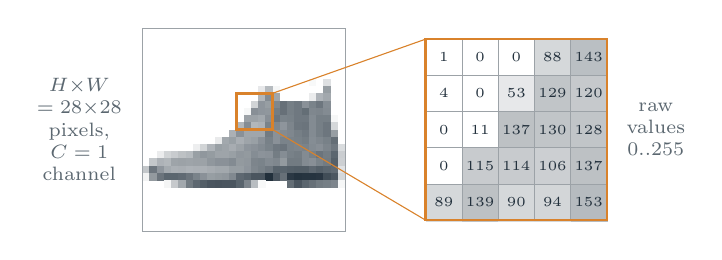
\begin{tikzpicture}[x=0.92mm,y=0.92mm]
  \fill[cInk!3] (23.00,-7.00) rectangle ++(1.04,-1.04);
\fill[cInk!15] (25.00,-7.00) rectangle ++(1.04,-1.04);
\fill[cInk!11] (16.00,-8.00) rectangle ++(1.04,-1.04);
\fill[cInk!33] (17.00,-8.00) rectangle ++(1.04,-1.04);
\fill[cInk!4] (18.00,-8.00) rectangle ++(1.04,-1.04);
\fill[cInk!47] (25.00,-8.00) rectangle ++(1.04,-1.04);
\fill[cInk!35] (16.00,-9.00) rectangle ++(1.04,-1.04);
\fill[cInk!56] (17.00,-9.00) rectangle ++(1.04,-1.04);
\fill[cInk!43] (18.00,-9.00) rectangle ++(1.04,-1.04);
\fill[cInk!9] (23.00,-9.00) rectangle ++(1.04,-1.04);
\fill[cInk!36] (24.00,-9.00) rectangle ++(1.04,-1.04);
\fill[cInk!42] (25.00,-9.00) rectangle ++(1.04,-1.04);
\fill[cInk!21] (15.00,-10.00) rectangle ++(1.04,-1.04);
\fill[cInk!51] (16.00,-10.00) rectangle ++(1.04,-1.04);
\fill[cInk!47] (17.00,-10.00) rectangle ++(1.04,-1.04);
\fill[cInk!58] (18.00,-10.00) rectangle ++(1.04,-1.04);
\fill[cInk!69] (19.00,-10.00) rectangle ++(1.04,-1.04);
\fill[cInk!62] (20.00,-10.00) rectangle ++(1.04,-1.04);
\fill[cInk!65] (21.00,-10.00) rectangle ++(1.04,-1.04);
\fill[cInk!53] (22.00,-10.00) rectangle ++(1.04,-1.04);
\fill[cInk!60] (23.00,-10.00) rectangle ++(1.04,-1.04);
\fill[cInk!66] (24.00,-10.00) rectangle ++(1.04,-1.04);
\fill[cInk!55] (25.00,-10.00) rectangle ++(1.04,-1.04);
\fill[cInk!4] (14.00,-11.00) rectangle ++(1.04,-1.04);
\fill[cInk!54] (15.00,-11.00) rectangle ++(1.04,-1.04);
\fill[cInk!51] (16.00,-11.00) rectangle ++(1.04,-1.04);
\fill[cInk!50] (17.00,-11.00) rectangle ++(1.04,-1.04);
\fill[cInk!63] (18.00,-11.00) rectangle ++(1.04,-1.04);
\fill[cInk!69] (19.00,-11.00) rectangle ++(1.04,-1.04);
\fill[cInk!62] (20.00,-11.00) rectangle ++(1.04,-1.04);
\fill[cInk!65] (21.00,-11.00) rectangle ++(1.04,-1.04);
\fill[cInk!70] (22.00,-11.00) rectangle ++(1.04,-1.04);
\fill[cInk!58] (23.00,-11.00) rectangle ++(1.04,-1.04);
\fill[cInk!59] (24.00,-11.00) rectangle ++(1.04,-1.04);
\fill[cInk!56] (25.00,-11.00) rectangle ++(1.04,-1.04);
\fill[cInk!45] (14.00,-12.00) rectangle ++(2.04,-1.04);
\fill[cInk!42] (16.00,-12.00) rectangle ++(1.04,-1.04);
\fill[cInk!54] (17.00,-12.00) rectangle ++(1.04,-1.04);
\fill[cInk!66] (18.00,-12.00) rectangle ++(1.04,-1.04);
\fill[cInk!60] (19.00,-12.00) rectangle ++(1.04,-1.04);
\fill[cInk!61] (20.00,-12.00) rectangle ++(1.04,-1.04);
\fill[cInk!65] (21.00,-12.00) rectangle ++(2.04,-1.04);
\fill[cInk!56] (23.00,-12.00) rectangle ++(1.04,-1.04);
\fill[cInk!62] (24.00,-12.00) rectangle ++(2.04,-1.04);
\fill[cInk!4] (26.00,-12.00) rectangle ++(1.04,-1.04);
\fill[cInk!35] (13.00,-13.00) rectangle ++(1.04,-1.04);
\fill[cInk!55] (14.00,-13.00) rectangle ++(1.04,-1.04);
\fill[cInk!35] (15.00,-13.00) rectangle ++(1.04,-1.04);
\fill[cInk!37] (16.00,-13.00) rectangle ++(1.04,-1.04);
\fill[cInk!60] (17.00,-13.00) rectangle ++(1.04,-1.04);
\fill[cInk!58] (18.00,-13.00) rectangle ++(1.04,-1.04);
\fill[cInk!51] (19.00,-13.00) rectangle ++(1.04,-1.04);
\fill[cInk!59] (20.00,-13.00) rectangle ++(1.04,-1.04);
\fill[cInk!66] (21.00,-13.00) rectangle ++(1.04,-1.04);
\fill[cInk!67] (22.00,-13.00) rectangle ++(1.04,-1.04);
\fill[cInk!56] (23.00,-13.00) rectangle ++(1.04,-1.04);
\fill[cInk!62] (24.00,-13.00) rectangle ++(1.04,-1.04);
\fill[cInk!66] (25.00,-13.00) rectangle ++(1.04,-1.04);
\fill[cInk!19] (26.00,-13.00) rectangle ++(1.04,-1.04);
\fill[cInk!38] (12.00,-14.00) rectangle ++(1.04,-1.04);
\fill[cInk!53] (13.00,-14.00) rectangle ++(1.04,-1.04);
\fill[cInk!43] (14.00,-14.00) rectangle ++(3.04,-1.04);
\fill[cInk!64] (17.00,-14.00) rectangle ++(1.04,-1.04);
\fill[cInk!53] (18.00,-14.00) rectangle ++(1.04,-1.04);
\fill[cInk!56] (19.00,-14.00) rectangle ++(1.04,-1.04);
\fill[cInk!58] (20.00,-14.00) rectangle ++(1.04,-1.04);
\fill[cInk!62] (21.00,-14.00) rectangle ++(1.04,-1.04);
\fill[cInk!65] (22.00,-14.00) rectangle ++(1.04,-1.04);
\fill[cInk!56] (23.00,-14.00) rectangle ++(1.04,-1.04);
\fill[cInk!62] (24.00,-14.00) rectangle ++(1.04,-1.04);
\fill[cInk!66] (25.00,-14.00) rectangle ++(1.04,-1.04);
\fill[cInk!47] (26.00,-14.00) rectangle ++(1.04,-1.04);
\fill[cInk!10] (10.00,-15.00) rectangle ++(1.04,-1.04);
\fill[cInk!42] (11.00,-15.00) rectangle ++(1.04,-1.04);
\fill[cInk!46] (12.00,-15.00) rectangle ++(1.04,-1.04);
\fill[cInk!39] (13.00,-15.00) rectangle ++(1.04,-1.04);
\fill[cInk!44] (14.00,-15.00) rectangle ++(1.04,-1.04);
\fill[cInk!46] (15.00,-15.00) rectangle ++(1.04,-1.04);
\fill[cInk!53] (16.00,-15.00) rectangle ++(1.04,-1.04);
\fill[cInk!61] (17.00,-15.00) rectangle ++(1.04,-1.04);
\fill[cInk!53] (18.00,-15.00) rectangle ++(1.04,-1.04);
\fill[cInk!60] (19.00,-15.00) rectangle ++(2.04,-1.04);
\fill[cInk!61] (21.00,-15.00) rectangle ++(1.04,-1.04);
\fill[cInk!63] (22.00,-15.00) rectangle ++(1.04,-1.04);
\fill[cInk!55] (23.00,-15.00) rectangle ++(1.04,-1.04);
\fill[cInk!58] (24.00,-15.00) rectangle ++(1.04,-1.04);
\fill[cInk!61] (25.00,-15.00) rectangle ++(1.04,-1.04);
\fill[cInk!70] (26.00,-15.00) rectangle ++(1.04,-1.04);
\fill[cInk!8] (7.00,-16.00) rectangle ++(1.04,-1.04);
\fill[cInk!21] (8.00,-16.00) rectangle ++(1.04,-1.04);
\fill[cInk!36] (9.00,-16.00) rectangle ++(1.04,-1.04);
\fill[cInk!46] (10.00,-16.00) rectangle ++(1.04,-1.04);
\fill[cInk!44] (11.00,-16.00) rectangle ++(1.04,-1.04);
\fill[cInk!40] (12.00,-16.00) rectangle ++(1.04,-1.04);
\fill[cInk!45] (13.00,-16.00) rectangle ++(1.04,-1.04);
\fill[cInk!51] (14.00,-16.00) rectangle ++(1.04,-1.04);
\fill[cInk!53] (15.00,-16.00) rectangle ++(1.04,-1.04);
\fill[cInk!56] (16.00,-16.00) rectangle ++(1.04,-1.04);
\fill[cInk!60] (17.00,-16.00) rectangle ++(1.04,-1.04);
\fill[cInk!65] (18.00,-16.00) rectangle ++(1.04,-1.04);
\fill[cInk!67] (19.00,-16.00) rectangle ++(1.04,-1.04);
\fill[cInk!60] (20.00,-16.00) rectangle ++(1.04,-1.04);
\fill[cInk!59] (21.00,-16.00) rectangle ++(1.04,-1.04);
\fill[cInk!60] (22.00,-16.00) rectangle ++(1.04,-1.04);
\fill[cInk!56] (23.00,-16.00) rectangle ++(1.04,-1.04);
\fill[cInk!54] (24.00,-16.00) rectangle ++(1.04,-1.04);
\fill[cInk!59] (25.00,-16.00) rectangle ++(1.04,-1.04);
\fill[cInk!65] (26.00,-16.00) rectangle ++(1.04,-1.04);
\fill[cInk!17] (27.00,-16.00) rectangle ++(1.04,-1.04);
\fill[cInk!9] (2.00,-17.00) rectangle ++(1.04,-1.04);
\fill[cInk!21] (3.00,-17.00) rectangle ++(1.04,-1.04);
\fill[cInk!25] (4.00,-17.00) rectangle ++(1.04,-1.04);
\fill[cInk!30] (5.00,-17.00) rectangle ++(1.04,-1.04);
\fill[cInk!33] (6.00,-17.00) rectangle ++(1.04,-1.04);
\fill[cInk!46] (7.00,-17.00) rectangle ++(1.04,-1.04);
\fill[cInk!50] (8.00,-17.00) rectangle ++(1.04,-1.04);
\fill[cInk!48] (9.00,-17.00) rectangle ++(1.04,-1.04);
\fill[cInk!44] (10.00,-17.00) rectangle ++(2.04,-1.04);
\fill[cInk!46] (12.00,-17.00) rectangle ++(1.04,-1.04);
\fill[cInk!50] (13.00,-17.00) rectangle ++(1.04,-1.04);
\fill[cInk!49] (14.00,-17.00) rectangle ++(1.04,-1.04);
\fill[cInk!55] (15.00,-17.00) rectangle ++(1.04,-1.04);
\fill[cInk!52] (16.00,-17.00) rectangle ++(1.04,-1.04);
\fill[cInk!53] (17.00,-17.00) rectangle ++(1.04,-1.04);
\fill[cInk!63] (18.00,-17.00) rectangle ++(1.04,-1.04);
\fill[cInk!55] (19.00,-17.00) rectangle ++(1.04,-1.04);
\fill[cInk!61] (20.00,-17.00) rectangle ++(1.04,-1.04);
\fill[cInk!63] (21.00,-17.00) rectangle ++(1.04,-1.04);
\fill[cInk!56] (22.00,-17.00) rectangle ++(1.04,-1.04);
\fill[cInk!61] (23.00,-17.00) rectangle ++(1.04,-1.04);
\fill[cInk!67] (24.00,-17.00) rectangle ++(1.04,-1.04);
\fill[cInk!63] (25.00,-17.00) rectangle ++(1.04,-1.04);
\fill[cInk!74] (26.00,-17.00) rectangle ++(1.04,-1.04);
\fill[cInk!24] (27.00,-17.00) rectangle ++(1.04,-1.04);
\fill[cInk!27] (1.00,-18.00) rectangle ++(1.04,-1.04);
\fill[cInk!37] (2.00,-18.00) rectangle ++(1.04,-1.04);
\fill[cInk!35] (3.00,-18.00) rectangle ++(1.04,-1.04);
\fill[cInk!44] (4.00,-18.00) rectangle ++(1.04,-1.04);
\fill[cInk!45] (5.00,-18.00) rectangle ++(1.04,-1.04);
\fill[cInk!44] (6.00,-18.00) rectangle ++(1.04,-1.04);
\fill[cInk!45] (7.00,-18.00) rectangle ++(2.04,-1.04);
\fill[cInk!50] (9.00,-18.00) rectangle ++(1.04,-1.04);
\fill[cInk!53] (10.00,-18.00) rectangle ++(2.04,-1.04);
\fill[cInk!56] (12.00,-18.00) rectangle ++(1.04,-1.04);
\fill[cInk!49] (13.00,-18.00) rectangle ++(1.04,-1.04);
\fill[cInk!50] (14.00,-18.00) rectangle ++(1.04,-1.04);
\fill[cInk!59] (15.00,-18.00) rectangle ++(1.04,-1.04);
\fill[cInk!60] (16.00,-18.00) rectangle ++(1.04,-1.04);
\fill[cInk!56] (17.00,-18.00) rectangle ++(1.04,-1.04);
\fill[cInk!58] (18.00,-18.00) rectangle ++(1.04,-1.04);
\fill[cInk!49] (19.00,-18.00) rectangle ++(1.04,-1.04);
\fill[cInk!64] (20.00,-18.00) rectangle ++(2.04,-1.04);
\fill[cInk!56] (22.00,-18.00) rectangle ++(1.04,-1.04);
\fill[cInk!54] (23.00,-18.00) rectangle ++(1.04,-1.04);
\fill[cInk!60] (24.00,-18.00) rectangle ++(1.04,-1.04);
\fill[cInk!64] (25.00,-18.00) rectangle ++(1.04,-1.04);
\fill[cInk!77] (26.00,-18.00) rectangle ++(1.04,-1.04);
\fill[cInk!23] (27.00,-18.00) rectangle ++(1.04,-1.04);
\fill[cInk!27] (0.00,-19.00) rectangle ++(1.04,-1.04);
\fill[cInk!66] (1.00,-19.00) rectangle ++(1.04,-1.04);
\fill[cInk!51] (2.00,-19.00) rectangle ++(1.04,-1.04);
\fill[cInk!41] (3.00,-19.00) rectangle ++(1.04,-1.04);
\fill[cInk!38] (4.00,-19.00) rectangle ++(1.04,-1.04);
\fill[cInk!39] (5.00,-19.00) rectangle ++(1.04,-1.04);
\fill[cInk!37] (6.00,-19.00) rectangle ++(1.04,-1.04);
\fill[cInk!38] (7.00,-19.00) rectangle ++(2.04,-1.04);
\fill[cInk!40] (9.00,-19.00) rectangle ++(1.04,-1.04);
\fill[cInk!42] (10.00,-19.00) rectangle ++(2.04,-1.04);
\fill[cInk!47] (12.00,-19.00) rectangle ++(2.04,-1.04);
\fill[cInk!51] (14.00,-19.00) rectangle ++(1.04,-1.04);
\fill[cInk!58] (15.00,-19.00) rectangle ++(1.04,-1.04);
\fill[cInk!61] (16.00,-19.00) rectangle ++(1.04,-1.04);
\fill[cInk!65] (17.00,-19.00) rectangle ++(1.04,-1.04);
\fill[cInk!75] (18.00,-19.00) rectangle ++(2.04,-1.04);
\fill[cInk!77] (20.00,-19.00) rectangle ++(1.04,-1.04);
\fill[cInk!78] (21.00,-19.00) rectangle ++(2.04,-1.04);
\fill[cInk!73] (23.00,-19.00) rectangle ++(1.04,-1.04);
\fill[cInk!77] (24.00,-19.00) rectangle ++(1.04,-1.04);
\fill[cInk!74] (25.00,-19.00) rectangle ++(1.04,-1.04);
\fill[cInk!72] (26.00,-19.00) rectangle ++(1.04,-1.04);
\fill[cInk!14] (27.00,-19.00) rectangle ++(1.04,-1.04);
\fill[cInk!6] (0.00,-20.00) rectangle ++(1.04,-1.04);
\fill[cInk!49] (1.00,-20.00) rectangle ++(1.04,-1.04);
\fill[cInk!67] (2.00,-20.00) rectangle ++(1.04,-1.04);
\fill[cInk!74] (3.00,-20.00) rectangle ++(2.04,-1.04);
\fill[cInk!72] (5.00,-20.00) rectangle ++(1.04,-1.04);
\fill[cInk!67] (6.00,-20.00) rectangle ++(1.04,-1.04);
\fill[cInk!60] (7.00,-20.00) rectangle ++(1.04,-1.04);
\fill[cInk!53] (8.00,-20.00) rectangle ++(1.04,-1.04);
\fill[cInk!47] (9.00,-20.00) rectangle ++(1.04,-1.04);
\fill[cInk!49] (10.00,-20.00) rectangle ++(1.04,-1.04);
\fill[cInk!50] (11.00,-20.00) rectangle ++(1.04,-1.04);
\fill[cInk!57] (12.00,-20.00) rectangle ++(1.04,-1.04);
\fill[cInk!73] (13.00,-20.00) rectangle ++(1.04,-1.04);
\fill[cInk!76] (14.00,-20.00) rectangle ++(1.04,-1.04);
\fill[cInk!82] (15.00,-20.00) rectangle ++(2.04,-1.04);
\fill[cInk!100] (17.00,-20.00) rectangle ++(1.04,-1.04);
\fill[cInk!82] (18.00,-20.00) rectangle ++(1.04,-1.04);
\fill[cInk!69] (19.00,-20.00) rectangle ++(1.04,-1.04);
\fill[cInk!96] (20.00,-20.00) rectangle ++(1.04,-1.04);
\fill[cInk!99] (21.00,-20.00) rectangle ++(1.04,-1.04);
\fill[cInk!98] (22.00,-20.00) rectangle ++(2.04,-1.04);
\fill[cInk!97] (24.00,-20.00) rectangle ++(1.04,-1.04);
\fill[cInk!86] (25.00,-20.00) rectangle ++(1.04,-1.04);
\fill[cInk!81] (26.00,-20.00) rectangle ++(1.04,-1.04);
\fill[cInk!19] (27.00,-20.00) rectangle ++(1.04,-1.04);
\fill[cInk!5] (3.00,-21.00) rectangle ++(1.04,-1.04);
\fill[cInk!26] (4.00,-21.00) rectangle ++(1.04,-1.04);
\fill[cInk!42] (5.00,-21.00) rectangle ++(1.04,-1.04);
\fill[cInk!64] (6.00,-21.00) rectangle ++(1.04,-1.04);
\fill[cInk!73] (7.00,-21.00) rectangle ++(1.04,-1.04);
\fill[cInk!78] (8.00,-21.00) rectangle ++(1.04,-1.04);
\fill[cInk!82] (9.00,-21.00) rectangle ++(1.04,-1.04);
\fill[cInk!83] (10.00,-21.00) rectangle ++(1.04,-1.04);
\fill[cInk!82] (11.00,-21.00) rectangle ++(2.04,-1.04);
\fill[cInk!75] (13.00,-21.00) rectangle ++(1.04,-1.04);
\fill[cInk!59] (14.00,-21.00) rectangle ++(1.04,-1.04);
\fill[cInk!32] (15.00,-21.00) rectangle ++(1.04,-1.04);
\fill[cInk!3] (16.00,-21.00) rectangle ++(1.04,-1.04);
\fill[cInk!70] (20.00,-21.00) rectangle ++(1.04,-1.04);
\fill[cInk!82] (21.00,-21.00) rectangle ++(1.04,-1.04);
\fill[cInk!74] (22.00,-21.00) rectangle ++(1.04,-1.04);
\fill[cInk!69] (23.00,-21.00) rectangle ++(1.04,-1.04);
\fill[cInk!64] (24.00,-21.00) rectangle ++(1.04,-1.04);
\fill[cInk!62] (25.00,-21.00) rectangle ++(1.04,-1.04);
\fill[cInk!59] (26.00,-21.00) rectangle ++(1.04,-1.04);
\fill[cInk!4] (27.00,-21.00) rectangle ++(1.04,-1.04);
\draw[cInk!45,line width=0.3pt] (0.00,0.00) rectangle ++(28,-28);

  \draw[cAtt,line width=0.9pt] (\patchCol,-\patchRow) rectangle ++(5,-5);
  \begin{scope}[xshift=36mm,yshift=-1.4mm,x=4.6mm,y=4.6mm,lab/.append style={font=\fontsize{5.4}{6}\selectfont}]
    \fill[cInk!19] (3.00,0.00) rectangle ++(1.04,-1.04);
\fill[cInk!31] (4.00,0.00) rectangle ++(1.04,-1.04);
\fill[cInk!11] (2.00,-1.00) rectangle ++(1.04,-1.04);
\fill[cInk!28] (3.00,-1.00) rectangle ++(1.04,-1.04);
\fill[cInk!26] (4.00,-1.00) rectangle ++(1.04,-1.04);
\fill[cInk!30] (2.00,-2.00) rectangle ++(1.04,-1.04);
\fill[cInk!28] (3.00,-2.00) rectangle ++(2.04,-1.04);
\fill[cInk!25] (1.00,-3.00) rectangle ++(2.04,-1.04);
\fill[cInk!23] (3.00,-3.00) rectangle ++(1.04,-1.04);
\fill[cInk!30] (4.00,-3.00) rectangle ++(1.04,-1.04);
\fill[cInk!19] (0.00,-4.00) rectangle ++(1.04,-1.04);
\fill[cInk!30] (1.00,-4.00) rectangle ++(1.04,-1.04);
\fill[cInk!19] (2.00,-4.00) rectangle ++(1.04,-1.04);
\fill[cInk!20] (3.00,-4.00) rectangle ++(1.04,-1.04);
\fill[cInk!33] (4.00,-4.00) rectangle ++(1.04,-1.04);
\node[lab] at (0.50,-0.50) {1};
\node[lab] at (1.50,-0.50) {0};
\node[lab] at (2.50,-0.50) {0};
\node[lab] at (3.50,-0.50) {88};
\node[lab] at (4.50,-0.50) {143};
\node[lab] at (0.50,-1.50) {4};
\node[lab] at (1.50,-1.50) {0};
\node[lab] at (2.50,-1.50) {53};
\node[lab] at (3.50,-1.50) {129};
\node[lab] at (4.50,-1.50) {120};
\node[lab] at (0.50,-2.50) {0};
\node[lab] at (1.50,-2.50) {11};
\node[lab] at (2.50,-2.50) {137};
\node[lab] at (3.50,-2.50) {130};
\node[lab] at (4.50,-2.50) {128};
\node[lab] at (0.50,-3.50) {0};
\node[lab] at (1.50,-3.50) {115};
\node[lab] at (2.50,-3.50) {114};
\node[lab] at (3.50,-3.50) {106};
\node[lab] at (4.50,-3.50) {137};
\node[lab] at (0.50,-4.50) {89};
\node[lab] at (1.50,-4.50) {139};
\node[lab] at (2.50,-4.50) {90};
\node[lab] at (3.50,-4.50) {94};
\node[lab] at (4.50,-4.50) {153};
\draw[cInk!45,line width=0.3pt,step=1] (0,0) grid (5,-5);

    \draw[cAtt,line width=0.9pt] (0,0) rectangle (5,-5);
    \coordinate (za) at (0,0); \coordinate (zb) at (0,-5);
  \end{scope}
  \draw[cAtt,line width=0.4pt] (\patchCol+5,-\patchRow) -- (za) (\patchCol+5,-\patchRow-5) -- (zb);
  \node[note,anchor=east] at (-1.5,-14) {$H{\times}W$\\$=28{\times}28$\\pixels,\\$C=1$\\channel};
  \node[note,anchor=west] at (65.5,-14) {raw\\values\\0..255};
\end{tikzpicture}

\vspace{0.3mm}
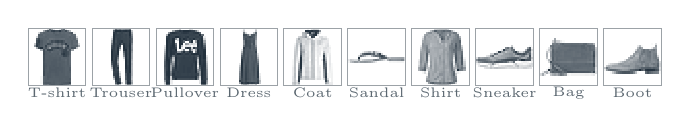
\begin{tikzpicture}[x=0.262mm,y=0.262mm,lab/.append style={font=\fontsize{4.6}{5}\selectfont,text=cTok}]
  \fill[cInk!20] (9.00,0.00) rectangle ++(1.04,-1.04);
\fill[cInk!75] (10.00,0.00) rectangle ++(1.04,-1.04);
\fill[cInk!45] (11.00,0.00) rectangle ++(1.04,-1.04);
\fill[cInk!11] (12.00,0.00) rectangle ++(1.04,-1.04);
\fill[cInk!12] (15.00,0.00) rectangle ++(1.04,-1.04);
\fill[cInk!56] (16.00,0.00) rectangle ++(1.04,-1.04);
\fill[cInk!70] (17.00,0.00) rectangle ++(1.04,-1.04);
\fill[cInk!13] (18.00,0.00) rectangle ++(1.04,-1.04);
\fill[cInk!44] (7.00,-1.00) rectangle ++(1.04,-1.04);
\fill[cInk!73] (8.00,-1.00) rectangle ++(1.04,-1.04);
\fill[cInk!85] (9.00,-1.00) rectangle ++(1.04,-1.04);
\fill[cInk!75] (10.00,-1.00) rectangle ++(1.04,-1.04);
\fill[cInk!90] (11.00,-1.00) rectangle ++(1.04,-1.04);
\fill[cInk!93] (12.00,-1.00) rectangle ++(1.04,-1.04);
\fill[cInk!86] (13.00,-1.00) rectangle ++(1.04,-1.04);
\fill[cInk!85] (14.00,-1.00) rectangle ++(1.04,-1.04);
\fill[cInk!95] (15.00,-1.00) rectangle ++(1.04,-1.04);
\fill[cInk!79] (16.00,-1.00) rectangle ++(1.04,-1.04);
\fill[cInk!75] (17.00,-1.00) rectangle ++(1.04,-1.04);
\fill[cInk!87] (18.00,-1.00) rectangle ++(1.04,-1.04);
\fill[cInk!65] (19.00,-1.00) rectangle ++(1.04,-1.04);
\fill[cInk!34] (20.00,-1.00) rectangle ++(1.04,-1.04);
\fill[cInk!20] (5.00,-2.00) rectangle ++(1.04,-1.04);
\fill[cInk!69] (6.00,-2.00) rectangle ++(1.04,-1.04);
\fill[cInk!76] (7.00,-2.00) rectangle ++(1.04,-1.04);
\fill[cInk!74] (8.00,-2.00) rectangle ++(1.04,-1.04);
\fill[cInk!73] (9.00,-2.00) rectangle ++(3.04,-1.04);
\fill[cInk!78] (12.00,-2.00) rectangle ++(1.04,-1.04);
\fill[cInk!74] (13.00,-2.00) rectangle ++(1.04,-1.04);
\fill[cInk!72] (14.00,-2.00) rectangle ++(1.04,-1.04);
\fill[cInk!76] (15.00,-2.00) rectangle ++(1.04,-1.04);
\fill[cInk!73] (16.00,-2.00) rectangle ++(1.04,-1.04);
\fill[cInk!74] (17.00,-2.00) rectangle ++(1.04,-1.04);
\fill[cInk!72] (18.00,-2.00) rectangle ++(1.04,-1.04);
\fill[cInk!73] (19.00,-2.00) rectangle ++(1.04,-1.04);
\fill[cInk!76] (20.00,-2.00) rectangle ++(1.04,-1.04);
\fill[cInk!82] (21.00,-2.00) rectangle ++(1.04,-1.04);
\fill[cInk!6] (22.00,-2.00) rectangle ++(1.04,-1.04);
\fill[cInk!78] (5.00,-3.00) rectangle ++(1.04,-1.04);
\fill[cInk!76] (6.00,-3.00) rectangle ++(1.04,-1.04);
\fill[cInk!71] (7.00,-3.00) rectangle ++(1.04,-1.04);
\fill[cInk!74] (8.00,-3.00) rectangle ++(1.04,-1.04);
\fill[cInk!75] (9.00,-3.00) rectangle ++(1.04,-1.04);
\fill[cInk!74] (10.00,-3.00) rectangle ++(2.04,-1.04);
\fill[cInk!75] (12.00,-3.00) rectangle ++(1.04,-1.04);
\fill[cInk!78] (13.00,-3.00) rectangle ++(1.04,-1.04);
\fill[cInk!77] (14.00,-3.00) rectangle ++(1.04,-1.04);
\fill[cInk!76] (15.00,-3.00) rectangle ++(1.04,-1.04);
\fill[cInk!75] (16.00,-3.00) rectangle ++(2.04,-1.04);
\fill[cInk!74] (18.00,-3.00) rectangle ++(1.04,-1.04);
\fill[cInk!72] (19.00,-3.00) rectangle ++(1.04,-1.04);
\fill[cInk!69] (20.00,-3.00) rectangle ++(1.04,-1.04);
\fill[cInk!74] (21.00,-3.00) rectangle ++(1.04,-1.04);
\fill[cInk!70] (22.00,-3.00) rectangle ++(1.04,-1.04);
\fill[cInk!19] (4.00,-4.00) rectangle ++(1.04,-1.04);
\fill[cInk!76] (5.00,-4.00) rectangle ++(1.04,-1.04);
\fill[cInk!74] (6.00,-4.00) rectangle ++(2.04,-1.04);
\fill[cInk!76] (8.00,-4.00) rectangle ++(1.04,-1.04);
\fill[cInk!74] (9.00,-4.00) rectangle ++(4.04,-1.04);
\fill[cInk!75] (13.00,-4.00) rectangle ++(3.04,-1.04);
\fill[cInk!76] (16.00,-4.00) rectangle ++(1.04,-1.04);
\fill[cInk!75] (17.00,-4.00) rectangle ++(1.04,-1.04);
\fill[cInk!74] (18.00,-4.00) rectangle ++(1.04,-1.04);
\fill[cInk!73] (19.00,-4.00) rectangle ++(1.04,-1.04);
\fill[cInk!76] (20.00,-4.00) rectangle ++(1.04,-1.04);
\fill[cInk!72] (21.00,-4.00) rectangle ++(1.04,-1.04);
\fill[cInk!74] (22.00,-4.00) rectangle ++(1.04,-1.04);
\fill[cInk!16] (23.00,-4.00) rectangle ++(1.04,-1.04);
\fill[cInk!76] (4.00,-5.00) rectangle ++(1.04,-1.04);
\fill[cInk!89] (5.00,-5.00) rectangle ++(1.04,-1.04);
\fill[cInk!77] (6.00,-5.00) rectangle ++(1.04,-1.04);
\fill[cInk!75] (7.00,-5.00) rectangle ++(1.04,-1.04);
\fill[cInk!74] (8.00,-5.00) rectangle ++(1.04,-1.04);
\fill[cInk!75] (9.00,-5.00) rectangle ++(1.04,-1.04);
\fill[cInk!69] (10.00,-5.00) rectangle ++(2.04,-1.04);
\fill[cInk!71] (12.00,-5.00) rectangle ++(1.04,-1.04);
\fill[cInk!73] (13.00,-5.00) rectangle ++(2.04,-1.04);
\fill[cInk!72] (15.00,-5.00) rectangle ++(1.04,-1.04);
\fill[cInk!71] (16.00,-5.00) rectangle ++(2.04,-1.04);
\fill[cInk!74] (18.00,-5.00) rectangle ++(1.04,-1.04);
\fill[cInk!75] (19.00,-5.00) rectangle ++(1.04,-1.04);
\fill[cInk!74] (20.00,-5.00) rectangle ++(1.04,-1.04);
\fill[cInk!73] (21.00,-5.00) rectangle ++(1.04,-1.04);
\fill[cInk!75] (22.00,-5.00) rectangle ++(1.04,-1.04);
\fill[cInk!49] (23.00,-5.00) rectangle ++(1.04,-1.04);
\fill[cInk!86] (4.00,-6.00) rectangle ++(1.04,-1.04);
\fill[cInk!93] (5.00,-6.00) rectangle ++(1.04,-1.04);
\fill[cInk!80] (6.00,-6.00) rectangle ++(1.04,-1.04);
\fill[cInk!75] (7.00,-6.00) rectangle ++(2.04,-1.04);
\fill[cInk!70] (9.00,-6.00) rectangle ++(1.04,-1.04);
\fill[cInk!75] (10.00,-6.00) rectangle ++(1.04,-1.04);
\fill[cInk!86] (11.00,-6.00) rectangle ++(1.04,-1.04);
\fill[cInk!82] (12.00,-6.00) rectangle ++(1.04,-1.04);
\fill[cInk!88] (13.00,-6.00) rectangle ++(1.04,-1.04);
\fill[cInk!91] (14.00,-6.00) rectangle ++(1.04,-1.04);
\fill[cInk!86] (15.00,-6.00) rectangle ++(1.04,-1.04);
\fill[cInk!89] (16.00,-6.00) rectangle ++(1.04,-1.04);
\fill[cInk!81] (17.00,-6.00) rectangle ++(1.04,-1.04);
\fill[cInk!72] (18.00,-6.00) rectangle ++(1.04,-1.04);
\fill[cInk!74] (19.00,-6.00) rectangle ++(2.04,-1.04);
\fill[cInk!77] (21.00,-6.00) rectangle ++(1.04,-1.04);
\fill[cInk!73] (22.00,-6.00) rectangle ++(1.04,-1.04);
\fill[cInk!75] (23.00,-6.00) rectangle ++(1.04,-1.04);
\fill[cInk!26] (3.00,-7.00) rectangle ++(1.04,-1.04);
\fill[cInk!92] (4.00,-7.00) rectangle ++(1.04,-1.04);
\fill[cInk!88] (5.00,-7.00) rectangle ++(1.04,-1.04);
\fill[cInk!79] (6.00,-7.00) rectangle ++(1.04,-1.04);
\fill[cInk!74] (7.00,-7.00) rectangle ++(1.04,-1.04);
\fill[cInk!75] (8.00,-7.00) rectangle ++(1.04,-1.04);
\fill[cInk!87] (9.00,-7.00) rectangle ++(1.04,-1.04);
\fill[cInk!84] (10.00,-7.00) rectangle ++(1.04,-1.04);
\fill[cInk!74] (11.00,-7.00) rectangle ++(1.04,-1.04);
\fill[cInk!63] (12.00,-7.00) rectangle ++(1.04,-1.04);
\fill[cInk!66] (13.00,-7.00) rectangle ++(1.04,-1.04);
\fill[cInk!75] (14.00,-7.00) rectangle ++(1.04,-1.04);
\fill[cInk!69] (15.00,-7.00) rectangle ++(1.04,-1.04);
\fill[cInk!81] (16.00,-7.00) rectangle ++(1.04,-1.04);
\fill[cInk!76] (17.00,-7.00) rectangle ++(1.04,-1.04);
\fill[cInk!94] (18.00,-7.00) rectangle ++(1.04,-1.04);
\fill[cInk!75] (19.00,-7.00) rectangle ++(1.04,-1.04);
\fill[cInk!73] (20.00,-7.00) rectangle ++(1.04,-1.04);
\fill[cInk!77] (21.00,-7.00) rectangle ++(1.04,-1.04);
\fill[cInk!72] (22.00,-7.00) rectangle ++(1.04,-1.04);
\fill[cInk!70] (23.00,-7.00) rectangle ++(1.04,-1.04);
\fill[cInk!18] (24.00,-7.00) rectangle ++(1.04,-1.04);
\fill[cInk!51] (3.00,-8.00) rectangle ++(1.04,-1.04);
\fill[cInk!95] (4.00,-8.00) rectangle ++(1.04,-1.04);
\fill[cInk!85] (5.00,-8.00) rectangle ++(1.04,-1.04);
\fill[cInk!78] (6.00,-8.00) rectangle ++(1.04,-1.04);
\fill[cInk!73] (7.00,-8.00) rectangle ++(1.04,-1.04);
\fill[cInk!90] (8.00,-8.00) rectangle ++(1.04,-1.04);
\fill[cInk!70] (9.00,-8.00) rectangle ++(1.04,-1.04);
\fill[cInk!67] (10.00,-8.00) rectangle ++(1.04,-1.04);
\fill[cInk!65] (11.00,-8.00) rectangle ++(1.04,-1.04);
\fill[cInk!63] (12.00,-8.00) rectangle ++(1.04,-1.04);
\fill[cInk!68] (13.00,-8.00) rectangle ++(1.04,-1.04);
\fill[cInk!69] (14.00,-8.00) rectangle ++(1.04,-1.04);
\fill[cInk!62] (15.00,-8.00) rectangle ++(1.04,-1.04);
\fill[cInk!69] (16.00,-8.00) rectangle ++(1.04,-1.04);
\fill[cInk!47] (17.00,-8.00) rectangle ++(1.04,-1.04);
\fill[cInk!70] (18.00,-8.00) rectangle ++(1.04,-1.04);
\fill[cInk!94] (19.00,-8.00) rectangle ++(1.04,-1.04);
\fill[cInk!71] (20.00,-8.00) rectangle ++(1.04,-1.04);
\fill[cInk!75] (21.00,-8.00) rectangle ++(2.04,-1.04);
\fill[cInk!77] (23.00,-8.00) rectangle ++(1.04,-1.04);
\fill[cInk!45] (24.00,-8.00) rectangle ++(1.04,-1.04);
\fill[cInk!42] (4.00,-9.00) rectangle ++(1.04,-1.04);
\fill[cInk!88] (5.00,-9.00) rectangle ++(1.04,-1.04);
\fill[cInk!100] (6.00,-9.00) rectangle ++(1.04,-1.04);
\fill[cInk!74] (7.00,-9.00) rectangle ++(1.04,-1.04);
\fill[cInk!83] (8.00,-9.00) rectangle ++(1.04,-1.04);
\fill[cInk!68] (9.00,-9.00) rectangle ++(1.04,-1.04);
\fill[cInk!48] (10.00,-9.00) rectangle ++(1.04,-1.04);
\fill[cInk!87] (11.00,-9.00) rectangle ++(2.04,-1.04);
\fill[cInk!89] (13.00,-9.00) rectangle ++(1.04,-1.04);
\fill[cInk!94] (14.00,-9.00) rectangle ++(1.04,-1.04);
\fill[cInk!85] (15.00,-9.00) rectangle ++(1.04,-1.04);
\fill[cInk!83] (16.00,-9.00) rectangle ++(1.04,-1.04);
\fill[cInk!59] (17.00,-9.00) rectangle ++(1.04,-1.04);
\fill[cInk!86] (18.00,-9.00) rectangle ++(1.04,-1.04);
\fill[cInk!84] (19.00,-9.00) rectangle ++(1.04,-1.04);
\fill[cInk!73] (20.00,-9.00) rectangle ++(1.04,-1.04);
\fill[cInk!84] (21.00,-9.00) rectangle ++(1.04,-1.04);
\fill[cInk!82] (22.00,-9.00) rectangle ++(1.04,-1.04);
\fill[cInk!28] (23.00,-9.00) rectangle ++(1.04,-1.04);
\fill[cInk!39] (6.00,-10.00) rectangle ++(1.04,-1.04);
\fill[cInk!86] (7.00,-10.00) rectangle ++(1.04,-1.04);
\fill[cInk!73] (8.00,-10.00) rectangle ++(1.04,-1.04);
\fill[cInk!89] (9.00,-10.00) rectangle ++(1.04,-1.04);
\fill[cInk!92] (10.00,-10.00) rectangle ++(1.04,-1.04);
\fill[cInk!89] (11.00,-10.00) rectangle ++(1.04,-1.04);
\fill[cInk!78] (12.00,-10.00) rectangle ++(1.04,-1.04);
\fill[cInk!75] (13.00,-10.00) rectangle ++(1.04,-1.04);
\fill[cInk!73] (14.00,-10.00) rectangle ++(1.04,-1.04);
\fill[cInk!77] (15.00,-10.00) rectangle ++(1.04,-1.04);
\fill[cInk!83] (16.00,-10.00) rectangle ++(1.04,-1.04);
\fill[cInk!88] (17.00,-10.00) rectangle ++(1.04,-1.04);
\fill[cInk!90] (18.00,-10.00) rectangle ++(1.04,-1.04);
\fill[cInk!72] (19.00,-10.00) rectangle ++(1.04,-1.04);
\fill[cInk!82] (20.00,-10.00) rectangle ++(1.04,-1.04);
\fill[cInk!45] (21.00,-10.00) rectangle ++(1.04,-1.04);
\fill[cInk!86] (7.00,-11.00) rectangle ++(1.04,-1.04);
\fill[cInk!78] (8.00,-11.00) rectangle ++(1.04,-1.04);
\fill[cInk!76] (9.00,-11.00) rectangle ++(1.04,-1.04);
\fill[cInk!80] (10.00,-11.00) rectangle ++(1.04,-1.04);
\fill[cInk!72] (11.00,-11.00) rectangle ++(1.04,-1.04);
\fill[cInk!75] (12.00,-11.00) rectangle ++(2.04,-1.04);
\fill[cInk!76] (14.00,-11.00) rectangle ++(1.04,-1.04);
\fill[cInk!74] (15.00,-11.00) rectangle ++(1.04,-1.04);
\fill[cInk!83] (16.00,-11.00) rectangle ++(1.04,-1.04);
\fill[cInk!91] (17.00,-11.00) rectangle ++(1.04,-1.04);
\fill[cInk!89] (18.00,-11.00) rectangle ++(1.04,-1.04);
\fill[cInk!85] (19.00,-11.00) rectangle ++(1.04,-1.04);
\fill[cInk!76] (20.00,-11.00) rectangle ++(1.04,-1.04);
\fill[cInk!87] (7.00,-12.00) rectangle ++(1.04,-1.04);
\fill[cInk!78] (8.00,-12.00) rectangle ++(1.04,-1.04);
\fill[cInk!77] (9.00,-12.00) rectangle ++(1.04,-1.04);
\fill[cInk!76] (10.00,-12.00) rectangle ++(1.04,-1.04);
\fill[cInk!77] (11.00,-12.00) rectangle ++(1.04,-1.04);
\fill[cInk!76] (12.00,-12.00) rectangle ++(2.04,-1.04);
\fill[cInk!78] (14.00,-12.00) rectangle ++(1.04,-1.04);
\fill[cInk!72] (15.00,-12.00) rectangle ++(1.04,-1.04);
\fill[cInk!89] (16.00,-12.00) rectangle ++(1.04,-1.04);
\fill[cInk!96] (17.00,-12.00) rectangle ++(1.04,-1.04);
\fill[cInk!89] (18.00,-12.00) rectangle ++(1.04,-1.04);
\fill[cInk!85] (19.00,-12.00) rectangle ++(1.04,-1.04);
\fill[cInk!76] (20.00,-12.00) rectangle ++(1.04,-1.04);
\fill[cInk!85] (7.00,-13.00) rectangle ++(1.04,-1.04);
\fill[cInk!77] (8.00,-13.00) rectangle ++(2.04,-1.04);
\fill[cInk!78] (10.00,-13.00) rectangle ++(1.04,-1.04);
\fill[cInk!77] (11.00,-13.00) rectangle ++(1.04,-1.04);
\fill[cInk!76] (12.00,-13.00) rectangle ++(1.04,-1.04);
\fill[cInk!77] (13.00,-13.00) rectangle ++(1.04,-1.04);
\fill[cInk!76] (14.00,-13.00) rectangle ++(2.04,-1.04);
\fill[cInk!79] (16.00,-13.00) rectangle ++(1.04,-1.04);
\fill[cInk!91] (17.00,-13.00) rectangle ++(1.04,-1.04);
\fill[cInk!89] (18.00,-13.00) rectangle ++(1.04,-1.04);
\fill[cInk!82] (19.00,-13.00) rectangle ++(1.04,-1.04);
\fill[cInk!72] (20.00,-13.00) rectangle ++(1.04,-1.04);
\fill[cInk!85] (7.00,-14.00) rectangle ++(1.04,-1.04);
\fill[cInk!77] (8.00,-14.00) rectangle ++(2.04,-1.04);
\fill[cInk!78] (10.00,-14.00) rectangle ++(4.04,-1.04);
\fill[cInk!77] (14.00,-14.00) rectangle ++(1.04,-1.04);
\fill[cInk!79] (15.00,-14.00) rectangle ++(1.04,-1.04);
\fill[cInk!75] (16.00,-14.00) rectangle ++(1.04,-1.04);
\fill[cInk!76] (17.00,-14.00) rectangle ++(2.04,-1.04);
\fill[cInk!77] (19.00,-14.00) rectangle ++(1.04,-1.04);
\fill[cInk!72] (20.00,-14.00) rectangle ++(1.04,-1.04);
\fill[cInk!84] (7.00,-15.00) rectangle ++(1.04,-1.04);
\fill[cInk!78] (8.00,-15.00) rectangle ++(4.04,-1.04);
\fill[cInk!79] (12.00,-15.00) rectangle ++(2.04,-1.04);
\fill[cInk!78] (14.00,-15.00) rectangle ++(1.04,-1.04);
\fill[cInk!79] (15.00,-15.00) rectangle ++(1.04,-1.04);
\fill[cInk!77] (16.00,-15.00) rectangle ++(1.04,-1.04);
\fill[cInk!76] (17.00,-15.00) rectangle ++(1.04,-1.04);
\fill[cInk!73] (18.00,-15.00) rectangle ++(1.04,-1.04);
\fill[cInk!78] (19.00,-15.00) rectangle ++(1.04,-1.04);
\fill[cInk!72] (20.00,-15.00) rectangle ++(1.04,-1.04);
\fill[cInk!83] (7.00,-16.00) rectangle ++(1.04,-1.04);
\fill[cInk!78] (8.00,-16.00) rectangle ++(3.04,-1.04);
\fill[cInk!79] (11.00,-16.00) rectangle ++(3.04,-1.04);
\fill[cInk!77] (14.00,-16.00) rectangle ++(1.04,-1.04);
\fill[cInk!78] (15.00,-16.00) rectangle ++(3.04,-1.04);
\fill[cInk!75] (18.00,-16.00) rectangle ++(1.04,-1.04);
\fill[cInk!78] (19.00,-16.00) rectangle ++(1.04,-1.04);
\fill[cInk!72] (20.00,-16.00) rectangle ++(1.04,-1.04);
\fill[cInk!84] (7.00,-17.00) rectangle ++(1.04,-1.04);
\fill[cInk!79] (8.00,-17.00) rectangle ++(1.04,-1.04);
\fill[cInk!78] (9.00,-17.00) rectangle ++(2.04,-1.04);
\fill[cInk!79] (11.00,-17.00) rectangle ++(3.04,-1.04);
\fill[cInk!78] (14.00,-17.00) rectangle ++(1.04,-1.04);
\fill[cInk!79] (15.00,-17.00) rectangle ++(1.04,-1.04);
\fill[cInk!78] (16.00,-17.00) rectangle ++(1.04,-1.04);
\fill[cInk!77] (17.00,-17.00) rectangle ++(1.04,-1.04);
\fill[cInk!75] (18.00,-17.00) rectangle ++(1.04,-1.04);
\fill[cInk!78] (19.00,-17.00) rectangle ++(1.04,-1.04);
\fill[cInk!73] (20.00,-17.00) rectangle ++(1.04,-1.04);
\fill[cInk!85] (7.00,-18.00) rectangle ++(1.04,-1.04);
\fill[cInk!80] (8.00,-18.00) rectangle ++(1.04,-1.04);
\fill[cInk!78] (9.00,-18.00) rectangle ++(1.04,-1.04);
\fill[cInk!79] (10.00,-18.00) rectangle ++(2.04,-1.04);
\fill[cInk!80] (12.00,-18.00) rectangle ++(1.04,-1.04);
\fill[cInk!79] (13.00,-18.00) rectangle ++(1.04,-1.04);
\fill[cInk!78] (14.00,-18.00) rectangle ++(1.04,-1.04);
\fill[cInk!79] (15.00,-18.00) rectangle ++(1.04,-1.04);
\fill[cInk!78] (16.00,-18.00) rectangle ++(1.04,-1.04);
\fill[cInk!77] (17.00,-18.00) rectangle ++(1.04,-1.04);
\fill[cInk!76] (18.00,-18.00) rectangle ++(1.04,-1.04);
\fill[cInk!77] (19.00,-18.00) rectangle ++(1.04,-1.04);
\fill[cInk!75] (20.00,-18.00) rectangle ++(1.04,-1.04);
\fill[cInk!85] (7.00,-19.00) rectangle ++(1.04,-1.04);
\fill[cInk!79] (8.00,-19.00) rectangle ++(1.04,-1.04);
\fill[cInk!77] (9.00,-19.00) rectangle ++(1.04,-1.04);
\fill[cInk!80] (10.00,-19.00) rectangle ++(1.04,-1.04);
\fill[cInk!79] (11.00,-19.00) rectangle ++(2.04,-1.04);
\fill[cInk!80] (13.00,-19.00) rectangle ++(2.04,-1.04);
\fill[cInk!79] (15.00,-19.00) rectangle ++(2.04,-1.04);
\fill[cInk!78] (17.00,-19.00) rectangle ++(1.04,-1.04);
\fill[cInk!76] (18.00,-19.00) rectangle ++(2.04,-1.04);
\fill[cInk!79] (20.00,-19.00) rectangle ++(1.04,-1.04);
\fill[cInk!85] (7.00,-20.00) rectangle ++(1.04,-1.04);
\fill[cInk!78] (8.00,-20.00) rectangle ++(1.04,-1.04);
\fill[cInk!77] (9.00,-20.00) rectangle ++(1.04,-1.04);
\fill[cInk!80] (10.00,-20.00) rectangle ++(4.04,-1.04);
\fill[cInk!79] (14.00,-20.00) rectangle ++(3.04,-1.04);
\fill[cInk!78] (17.00,-20.00) rectangle ++(1.04,-1.04);
\fill[cInk!76] (18.00,-20.00) rectangle ++(2.04,-1.04);
\fill[cInk!80] (20.00,-20.00) rectangle ++(1.04,-1.04);
\fill[cInk!87] (7.00,-21.00) rectangle ++(1.04,-1.04);
\fill[cInk!78] (8.00,-21.00) rectangle ++(2.04,-1.04);
\fill[cInk!80] (10.00,-21.00) rectangle ++(1.04,-1.04);
\fill[cInk!79] (11.00,-21.00) rectangle ++(2.04,-1.04);
\fill[cInk!80] (13.00,-21.00) rectangle ++(1.04,-1.04);
\fill[cInk!79] (14.00,-21.00) rectangle ++(1.04,-1.04);
\fill[cInk!78] (15.00,-21.00) rectangle ++(1.04,-1.04);
\fill[cInk!79] (16.00,-21.00) rectangle ++(1.04,-1.04);
\fill[cInk!78] (17.00,-21.00) rectangle ++(1.04,-1.04);
\fill[cInk!76] (18.00,-21.00) rectangle ++(1.04,-1.04);
\fill[cInk!77] (19.00,-21.00) rectangle ++(1.04,-1.04);
\fill[cInk!78] (20.00,-21.00) rectangle ++(1.04,-1.04);
\fill[cInk!88] (7.00,-22.00) rectangle ++(1.04,-1.04);
\fill[cInk!78] (8.00,-22.00) rectangle ++(1.04,-1.04);
\fill[cInk!79] (9.00,-22.00) rectangle ++(2.04,-1.04);
\fill[cInk!78] (11.00,-22.00) rectangle ++(2.04,-1.04);
\fill[cInk!79] (13.00,-22.00) rectangle ++(2.04,-1.04);
\fill[cInk!78] (15.00,-22.00) rectangle ++(3.04,-1.04);
\fill[cInk!76] (18.00,-22.00) rectangle ++(1.04,-1.04);
\fill[cInk!77] (19.00,-22.00) rectangle ++(1.04,-1.04);
\fill[cInk!76] (20.00,-22.00) rectangle ++(1.04,-1.04);
\fill[cInk!4] (6.00,-23.00) rectangle ++(1.04,-1.04);
\fill[cInk!75] (7.00,-23.00) rectangle ++(1.04,-1.04);
\fill[cInk!76] (8.00,-23.00) rectangle ++(1.04,-1.04);
\fill[cInk!80] (9.00,-23.00) rectangle ++(1.04,-1.04);
\fill[cInk!79] (10.00,-23.00) rectangle ++(1.04,-1.04);
\fill[cInk!78] (11.00,-23.00) rectangle ++(1.04,-1.04);
\fill[cInk!77] (12.00,-23.00) rectangle ++(1.04,-1.04);
\fill[cInk!78] (13.00,-23.00) rectangle ++(7.04,-1.04);
\fill[cInk!76] (20.00,-23.00) rectangle ++(1.04,-1.04);
\fill[cInk!4] (6.00,-24.00) rectangle ++(1.04,-1.04);
\fill[cInk!76] (7.00,-24.00) rectangle ++(1.04,-1.04);
\fill[cInk!77] (8.00,-24.00) rectangle ++(1.04,-1.04);
\fill[cInk!79] (9.00,-24.00) rectangle ++(1.04,-1.04);
\fill[cInk!77] (10.00,-24.00) rectangle ++(5.04,-1.04);
\fill[cInk!78] (15.00,-24.00) rectangle ++(2.04,-1.04);
\fill[cInk!77] (17.00,-24.00) rectangle ++(1.04,-1.04);
\fill[cInk!78] (18.00,-24.00) rectangle ++(2.04,-1.04);
\fill[cInk!80] (20.00,-24.00) rectangle ++(1.04,-1.04);
\fill[cInk!4] (6.00,-25.00) rectangle ++(1.04,-1.04);
\fill[cInk!75] (7.00,-25.00) rectangle ++(1.04,-1.04);
\fill[cInk!77] (8.00,-25.00) rectangle ++(1.04,-1.04);
\fill[cInk!76] (9.00,-25.00) rectangle ++(3.04,-1.04);
\fill[cInk!77] (12.00,-25.00) rectangle ++(1.04,-1.04);
\fill[cInk!76] (13.00,-25.00) rectangle ++(2.04,-1.04);
\fill[cInk!77] (15.00,-25.00) rectangle ++(3.04,-1.04);
\fill[cInk!76] (18.00,-25.00) rectangle ++(1.04,-1.04);
\fill[cInk!77] (19.00,-25.00) rectangle ++(1.04,-1.04);
\fill[cInk!78] (20.00,-25.00) rectangle ++(1.04,-1.04);
\fill[cInk!4] (6.00,-26.00) rectangle ++(1.04,-1.04);
\fill[cInk!78] (7.00,-26.00) rectangle ++(1.04,-1.04);
\fill[cInk!80] (8.00,-26.00) rectangle ++(2.04,-1.04);
\fill[cInk!79] (10.00,-26.00) rectangle ++(1.04,-1.04);
\fill[cInk!77] (11.00,-26.00) rectangle ++(1.04,-1.04);
\fill[cInk!78] (12.00,-26.00) rectangle ++(1.04,-1.04);
\fill[cInk!76] (13.00,-26.00) rectangle ++(1.04,-1.04);
\fill[cInk!75] (14.00,-26.00) rectangle ++(1.04,-1.04);
\fill[cInk!76] (15.00,-26.00) rectangle ++(1.04,-1.04);
\fill[cInk!78] (16.00,-26.00) rectangle ++(1.04,-1.04);
\fill[cInk!79] (17.00,-26.00) rectangle ++(1.04,-1.04);
\fill[cInk!80] (18.00,-26.00) rectangle ++(1.04,-1.04);
\fill[cInk!81] (19.00,-26.00) rectangle ++(1.04,-1.04);
\fill[cInk!87] (20.00,-26.00) rectangle ++(1.04,-1.04);
\fill[cInk!69] (7.00,-27.00) rectangle ++(1.04,-1.04);
\fill[cInk!71] (8.00,-27.00) rectangle ++(1.04,-1.04);
\fill[cInk!66] (9.00,-27.00) rectangle ++(1.04,-1.04);
\fill[cInk!76] (10.00,-27.00) rectangle ++(1.04,-1.04);
\fill[cInk!79] (11.00,-27.00) rectangle ++(2.04,-1.04);
\fill[cInk!76] (13.00,-27.00) rectangle ++(2.04,-1.04);
\fill[cInk!79] (15.00,-27.00) rectangle ++(1.04,-1.04);
\fill[cInk!81] (16.00,-27.00) rectangle ++(1.04,-1.04);
\fill[cInk!76] (17.00,-27.00) rectangle ++(1.04,-1.04);
\fill[cInk!73] (18.00,-27.00) rectangle ++(1.04,-1.04);
\fill[cInk!68] (19.00,-27.00) rectangle ++(1.04,-1.04);
\fill[cInk!58] (20.00,-27.00) rectangle ++(1.04,-1.04);
\draw[cInk!45,line width=0.3pt] (0.00,0.00) rectangle ++(28,-28);
\node[lab] at (14.00,-31.50) {T-shirt};
\fill[cInk!26] (41.00,0.00) rectangle ++(1.04,-1.04);
\fill[cInk!69] (42.00,0.00) rectangle ++(1.04,-1.04);
\fill[cInk!51] (43.00,0.00) rectangle ++(1.04,-1.04);
\fill[cInk!60] (44.00,0.00) rectangle ++(1.04,-1.04);
\fill[cInk!46] (45.00,0.00) rectangle ++(1.04,-1.04);
\fill[cInk!51] (46.00,0.00) rectangle ++(1.04,-1.04);
\fill[cInk!57] (47.00,0.00) rectangle ++(1.04,-1.04);
\fill[cInk!55] (48.00,0.00) rectangle ++(1.04,-1.04);
\fill[cInk!69] (49.00,0.00) rectangle ++(1.04,-1.04);
\fill[cInk!77] (41.00,-1.00) rectangle ++(1.04,-1.04);
\fill[cInk!100] (42.00,-1.00) rectangle ++(3.04,-1.04);
\fill[cInk!95] (45.00,-1.00) rectangle ++(1.04,-1.04);
\fill[cInk!98] (46.00,-1.00) rectangle ++(1.04,-1.04);
\fill[cInk!100] (47.00,-1.00) rectangle ++(1.04,-1.04);
\fill[cInk!96] (48.00,-1.00) rectangle ++(1.04,-1.04);
\fill[cInk!100] (49.00,-1.00) rectangle ++(1.04,-1.04);
\fill[cInk!30] (50.00,-1.00) rectangle ++(1.04,-1.04);
\fill[cInk!95] (41.00,-2.00) rectangle ++(1.04,-1.04);
\fill[cInk!93] (42.00,-2.00) rectangle ++(1.04,-1.04);
\fill[cInk!85] (43.00,-2.00) rectangle ++(1.04,-1.04);
\fill[cInk!89] (44.00,-2.00) rectangle ++(1.04,-1.04);
\fill[cInk!91] (45.00,-2.00) rectangle ++(1.04,-1.04);
\fill[cInk!87] (46.00,-2.00) rectangle ++(1.04,-1.04);
\fill[cInk!85] (47.00,-2.00) rectangle ++(1.04,-1.04);
\fill[cInk!86] (48.00,-2.00) rectangle ++(1.04,-1.04);
\fill[cInk!100] (49.00,-2.00) rectangle ++(1.04,-1.04);
\fill[cInk!45] (50.00,-2.00) rectangle ++(1.04,-1.04);
\fill[cInk!100] (41.00,-3.00) rectangle ++(1.04,-1.04);
\fill[cInk!92] (42.00,-3.00) rectangle ++(1.04,-1.04);
\fill[cInk!91] (43.00,-3.00) rectangle ++(2.04,-1.04);
\fill[cInk!89] (45.00,-3.00) rectangle ++(1.04,-1.04);
\fill[cInk!88] (46.00,-3.00) rectangle ++(1.04,-1.04);
\fill[cInk!90] (47.00,-3.00) rectangle ++(1.04,-1.04);
\fill[cInk!87] (48.00,-3.00) rectangle ++(1.04,-1.04);
\fill[cInk!100] (49.00,-3.00) rectangle ++(1.04,-1.04);
\fill[cInk!57] (50.00,-3.00) rectangle ++(1.04,-1.04);
\fill[cInk!9] (40.00,-4.00) rectangle ++(1.04,-1.04);
\fill[cInk!100] (41.00,-4.00) rectangle ++(1.04,-1.04);
\fill[cInk!90] (42.00,-4.00) rectangle ++(2.04,-1.04);
\fill[cInk!91] (44.00,-4.00) rectangle ++(1.04,-1.04);
\fill[cInk!90] (45.00,-4.00) rectangle ++(1.04,-1.04);
\fill[cInk!88] (46.00,-4.00) rectangle ++(1.04,-1.04);
\fill[cInk!89] (47.00,-4.00) rectangle ++(1.04,-1.04);
\fill[cInk!87] (48.00,-4.00) rectangle ++(1.04,-1.04);
\fill[cInk!95] (49.00,-4.00) rectangle ++(1.04,-1.04);
\fill[cInk!65] (50.00,-4.00) rectangle ++(1.04,-1.04);
\fill[cInk!26] (40.00,-5.00) rectangle ++(1.04,-1.04);
\fill[cInk!100] (41.00,-5.00) rectangle ++(1.04,-1.04);
\fill[cInk!88] (42.00,-5.00) rectangle ++(1.04,-1.04);
\fill[cInk!92] (43.00,-5.00) rectangle ++(1.04,-1.04);
\fill[cInk!91] (44.00,-5.00) rectangle ++(1.04,-1.04);
\fill[cInk!89] (45.00,-5.00) rectangle ++(3.04,-1.04);
\fill[cInk!88] (48.00,-5.00) rectangle ++(1.04,-1.04);
\fill[cInk!92] (49.00,-5.00) rectangle ++(1.04,-1.04);
\fill[cInk!73] (50.00,-5.00) rectangle ++(1.04,-1.04);
\fill[cInk!45] (40.00,-6.00) rectangle ++(1.04,-1.04);
\fill[cInk!98] (41.00,-6.00) rectangle ++(1.04,-1.04);
\fill[cInk!85] (42.00,-6.00) rectangle ++(1.04,-1.04);
\fill[cInk!92] (43.00,-6.00) rectangle ++(1.04,-1.04);
\fill[cInk!93] (44.00,-6.00) rectangle ++(1.04,-1.04);
\fill[cInk!96] (45.00,-6.00) rectangle ++(1.04,-1.04);
\fill[cInk!89] (46.00,-6.00) rectangle ++(2.04,-1.04);
\fill[cInk!88] (48.00,-6.00) rectangle ++(1.04,-1.04);
\fill[cInk!95] (49.00,-6.00) rectangle ++(1.04,-1.04);
\fill[cInk!69] (50.00,-6.00) rectangle ++(1.04,-1.04);
\fill[cInk!65] (40.00,-7.00) rectangle ++(1.04,-1.04);
\fill[cInk!97] (41.00,-7.00) rectangle ++(1.04,-1.04);
\fill[cInk!89] (42.00,-7.00) rectangle ++(1.04,-1.04);
\fill[cInk!91] (43.00,-7.00) rectangle ++(1.04,-1.04);
\fill[cInk!98] (44.00,-7.00) rectangle ++(1.04,-1.04);
\fill[cInk!78] (45.00,-7.00) rectangle ++(1.04,-1.04);
\fill[cInk!97] (46.00,-7.00) rectangle ++(1.04,-1.04);
\fill[cInk!91] (47.00,-7.00) rectangle ++(1.04,-1.04);
\fill[cInk!88] (48.00,-7.00) rectangle ++(1.04,-1.04);
\fill[cInk!98] (49.00,-7.00) rectangle ++(1.04,-1.04);
\fill[cInk!58] (50.00,-7.00) rectangle ++(1.04,-1.04);
\fill[cInk!82] (40.00,-8.00) rectangle ++(1.04,-1.04);
\fill[cInk!95] (41.00,-8.00) rectangle ++(1.04,-1.04);
\fill[cInk!88] (42.00,-8.00) rectangle ++(1.04,-1.04);
\fill[cInk!95] (43.00,-8.00) rectangle ++(1.04,-1.04);
\fill[cInk!88] (44.00,-8.00) rectangle ++(1.04,-1.04);
\fill[cInk!100] (46.00,-8.00) rectangle ++(1.04,-1.04);
\fill[cInk!91] (47.00,-8.00) rectangle ++(1.04,-1.04);
\fill[cInk!89] (48.00,-8.00) rectangle ++(1.04,-1.04);
\fill[cInk!100] (49.00,-8.00) rectangle ++(1.04,-1.04);
\fill[cInk!51] (50.00,-8.00) rectangle ++(1.04,-1.04);
\fill[cInk!87] (40.00,-9.00) rectangle ++(1.04,-1.04);
\fill[cInk!93] (41.00,-9.00) rectangle ++(1.04,-1.04);
\fill[cInk!87] (42.00,-9.00) rectangle ++(1.04,-1.04);
\fill[cInk!100] (43.00,-9.00) rectangle ++(1.04,-1.04);
\fill[cInk!63] (44.00,-9.00) rectangle ++(1.04,-1.04);
\fill[cInk!100] (46.00,-9.00) rectangle ++(1.04,-1.04);
\fill[cInk!93] (47.00,-9.00) rectangle ++(1.04,-1.04);
\fill[cInk!87] (48.00,-9.00) rectangle ++(1.04,-1.04);
\fill[cInk!100] (49.00,-9.00) rectangle ++(1.04,-1.04);
\fill[cInk!53] (50.00,-9.00) rectangle ++(1.04,-1.04);
\fill[cInk!96] (40.00,-10.00) rectangle ++(1.04,-1.04);
\fill[cInk!92] (41.00,-10.00) rectangle ++(1.04,-1.04);
\fill[cInk!87] (42.00,-10.00) rectangle ++(1.04,-1.04);
\fill[cInk!100] (43.00,-10.00) rectangle ++(1.04,-1.04);
\fill[cInk!28] (44.00,-10.00) rectangle ++(1.04,-1.04);
\fill[cInk!97] (46.00,-10.00) rectangle ++(1.04,-1.04);
\fill[cInk!100] (47.00,-10.00) rectangle ++(1.04,-1.04);
\fill[cInk!85] (48.00,-10.00) rectangle ++(1.04,-1.04);
\fill[cInk!100] (49.00,-10.00) rectangle ++(1.04,-1.04);
\fill[cInk!57] (50.00,-10.00) rectangle ++(1.04,-1.04);
\fill[cInk!100] (40.00,-11.00) rectangle ++(1.04,-1.04);
\fill[cInk!91] (41.00,-11.00) rectangle ++(1.04,-1.04);
\fill[cInk!89] (42.00,-11.00) rectangle ++(1.04,-1.04);
\fill[cInk!100] (43.00,-11.00) rectangle ++(1.04,-1.04);
\fill[cInk!3] (44.00,-11.00) rectangle ++(1.04,-1.04);
\fill[cInk!75] (46.00,-11.00) rectangle ++(1.04,-1.04);
\fill[cInk!97] (47.00,-11.00) rectangle ++(1.04,-1.04);
\fill[cInk!86] (48.00,-11.00) rectangle ++(1.04,-1.04);
\fill[cInk!100] (49.00,-11.00) rectangle ++(1.04,-1.04);
\fill[cInk!49] (50.00,-11.00) rectangle ++(1.04,-1.04);
\fill[cInk!100] (40.00,-12.00) rectangle ++(1.04,-1.04);
\fill[cInk!91] (41.00,-12.00) rectangle ++(2.04,-1.04);
\fill[cInk!98] (43.00,-12.00) rectangle ++(1.04,-1.04);
\fill[cInk!62] (46.00,-12.00) rectangle ++(1.04,-1.04);
\fill[cInk!98] (47.00,-12.00) rectangle ++(1.04,-1.04);
\fill[cInk!87] (48.00,-12.00) rectangle ++(1.04,-1.04);
\fill[cInk!100] (49.00,-12.00) rectangle ++(1.04,-1.04);
\fill[cInk!44] (50.00,-12.00) rectangle ++(1.04,-1.04);
\fill[cInk!100] (40.00,-13.00) rectangle ++(1.04,-1.04);
\fill[cInk!91] (41.00,-13.00) rectangle ++(1.04,-1.04);
\fill[cInk!93] (42.00,-13.00) rectangle ++(1.04,-1.04);
\fill[cInk!85] (43.00,-13.00) rectangle ++(1.04,-1.04);
\fill[cInk!51] (46.00,-13.00) rectangle ++(1.04,-1.04);
\fill[cInk!99] (47.00,-13.00) rectangle ++(1.04,-1.04);
\fill[cInk!86] (48.00,-13.00) rectangle ++(1.04,-1.04);
\fill[cInk!100] (49.00,-13.00) rectangle ++(1.04,-1.04);
\fill[cInk!44] (50.00,-13.00) rectangle ++(1.04,-1.04);
\fill[cInk!100] (40.00,-14.00) rectangle ++(1.04,-1.04);
\fill[cInk!89] (41.00,-14.00) rectangle ++(1.04,-1.04);
\fill[cInk!95] (42.00,-14.00) rectangle ++(1.04,-1.04);
\fill[cInk!67] (43.00,-14.00) rectangle ++(1.04,-1.04);
\fill[cInk!22] (46.00,-14.00) rectangle ++(1.04,-1.04);
\fill[cInk!98] (47.00,-14.00) rectangle ++(1.04,-1.04);
\fill[cInk!87] (48.00,-14.00) rectangle ++(1.04,-1.04);
\fill[cInk!100] (49.00,-14.00) rectangle ++(1.04,-1.04);
\fill[cInk!44] (50.00,-14.00) rectangle ++(1.04,-1.04);
\fill[cInk!100] (40.00,-15.00) rectangle ++(1.04,-1.04);
\fill[cInk!90] (41.00,-15.00) rectangle ++(1.04,-1.04);
\fill[cInk!96] (42.00,-15.00) rectangle ++(1.04,-1.04);
\fill[cInk!55] (43.00,-15.00) rectangle ++(1.04,-1.04);
\fill[cInk!4] (46.00,-15.00) rectangle ++(1.04,-1.04);
\fill[cInk!100] (47.00,-15.00) rectangle ++(1.04,-1.04);
\fill[cInk!89] (48.00,-15.00) rectangle ++(1.04,-1.04);
\fill[cInk!100] (49.00,-15.00) rectangle ++(1.04,-1.04);
\fill[cInk!39] (50.00,-15.00) rectangle ++(1.04,-1.04);
\fill[cInk!89] (40.00,-16.00) rectangle ++(1.04,-1.04);
\fill[cInk!93] (41.00,-16.00) rectangle ++(1.04,-1.04);
\fill[cInk!95] (42.00,-16.00) rectangle ++(1.04,-1.04);
\fill[cInk!44] (43.00,-16.00) rectangle ++(1.04,-1.04);
\fill[cInk!100] (47.00,-16.00) rectangle ++(1.04,-1.04);
\fill[cInk!90] (48.00,-16.00) rectangle ++(1.04,-1.04);
\fill[cInk!100] (49.00,-16.00) rectangle ++(1.04,-1.04);
\fill[cInk!35] (50.00,-16.00) rectangle ++(1.04,-1.04);
\fill[cInk!80] (40.00,-17.00) rectangle ++(1.04,-1.04);
\fill[cInk!94] (41.00,-17.00) rectangle ++(1.04,-1.04);
\fill[cInk!96] (42.00,-17.00) rectangle ++(1.04,-1.04);
\fill[cInk!59] (43.00,-17.00) rectangle ++(1.04,-1.04);
\fill[cInk!100] (47.00,-17.00) rectangle ++(1.04,-1.04);
\fill[cInk!89] (48.00,-17.00) rectangle ++(1.04,-1.04);
\fill[cInk!100] (49.00,-17.00) rectangle ++(1.04,-1.04);
\fill[cInk!39] (50.00,-17.00) rectangle ++(1.04,-1.04);
\fill[cInk!59] (40.00,-18.00) rectangle ++(1.04,-1.04);
\fill[cInk!96] (41.00,-18.00) rectangle ++(1.04,-1.04);
\fill[cInk!93] (42.00,-18.00) rectangle ++(1.04,-1.04);
\fill[cInk!78] (43.00,-18.00) rectangle ++(1.04,-1.04);
\fill[cInk!100] (47.00,-18.00) rectangle ++(1.04,-1.04);
\fill[cInk!92] (48.00,-18.00) rectangle ++(1.04,-1.04);
\fill[cInk!100] (49.00,-18.00) rectangle ++(1.04,-1.04);
\fill[cInk!36] (50.00,-18.00) rectangle ++(1.04,-1.04);
\fill[cInk!35] (40.00,-19.00) rectangle ++(1.04,-1.04);
\fill[cInk!97] (41.00,-19.00) rectangle ++(1.04,-1.04);
\fill[cInk!91] (42.00,-19.00) rectangle ++(1.04,-1.04);
\fill[cInk!97] (43.00,-19.00) rectangle ++(1.04,-1.04);
\fill[cInk!99] (47.00,-19.00) rectangle ++(1.04,-1.04);
\fill[cInk!93] (48.00,-19.00) rectangle ++(1.04,-1.04);
\fill[cInk!100] (49.00,-19.00) rectangle ++(1.04,-1.04);
\fill[cInk!35] (50.00,-19.00) rectangle ++(1.04,-1.04);
\fill[cInk!12] (40.00,-20.00) rectangle ++(1.04,-1.04);
\fill[cInk!94] (41.00,-20.00) rectangle ++(1.04,-1.04);
\fill[cInk!90] (42.00,-20.00) rectangle ++(1.04,-1.04);
\fill[cInk!89] (43.00,-20.00) rectangle ++(1.04,-1.04);
\fill[cInk!94] (47.00,-20.00) rectangle ++(1.04,-1.04);
\fill[cInk!93] (48.00,-20.00) rectangle ++(1.04,-1.04);
\fill[cInk!100] (49.00,-20.00) rectangle ++(1.04,-1.04);
\fill[cInk!36] (50.00,-20.00) rectangle ++(1.04,-1.04);
\fill[cInk!89] (41.00,-21.00) rectangle ++(1.04,-1.04);
\fill[cInk!91] (42.00,-21.00) rectangle ++(1.04,-1.04);
\fill[cInk!93] (43.00,-21.00) rectangle ++(1.04,-1.04);
\fill[cInk!13] (44.00,-21.00) rectangle ++(1.04,-1.04);
\fill[cInk!92] (47.00,-21.00) rectangle ++(1.04,-1.04);
\fill[cInk!93] (48.00,-21.00) rectangle ++(1.04,-1.04);
\fill[cInk!100] (49.00,-21.00) rectangle ++(1.04,-1.04);
\fill[cInk!37] (50.00,-21.00) rectangle ++(1.04,-1.04);
\fill[cInk!91] (41.00,-22.00) rectangle ++(1.04,-1.04);
\fill[cInk!93] (42.00,-22.00) rectangle ++(1.04,-1.04);
\fill[cInk!96] (43.00,-22.00) rectangle ++(1.04,-1.04);
\fill[cInk!27] (44.00,-22.00) rectangle ++(1.04,-1.04);
\fill[cInk!82] (47.00,-22.00) rectangle ++(1.04,-1.04);
\fill[cInk!95] (48.00,-22.00) rectangle ++(1.04,-1.04);
\fill[cInk!93] (49.00,-22.00) rectangle ++(1.04,-1.04);
\fill[cInk!38] (50.00,-22.00) rectangle ++(1.04,-1.04);
\fill[cInk!60] (41.00,-23.00) rectangle ++(1.04,-1.04);
\fill[cInk!95] (42.00,-23.00) rectangle ++(1.04,-1.04);
\fill[cInk!96] (43.00,-23.00) rectangle ++(1.04,-1.04);
\fill[cInk!50] (44.00,-23.00) rectangle ++(1.04,-1.04);
\fill[cInk!78] (47.00,-23.00) rectangle ++(1.04,-1.04);
\fill[cInk!95] (48.00,-23.00) rectangle ++(1.04,-1.04);
\fill[cInk!93] (49.00,-23.00) rectangle ++(1.04,-1.04);
\fill[cInk!32] (50.00,-23.00) rectangle ++(1.04,-1.04);
\fill[cInk!29] (41.00,-24.00) rectangle ++(1.04,-1.04);
\fill[cInk!96] (42.00,-24.00) rectangle ++(1.04,-1.04);
\fill[cInk!95] (43.00,-24.00) rectangle ++(1.04,-1.04);
\fill[cInk!83] (44.00,-24.00) rectangle ++(1.04,-1.04);
\fill[cInk!79] (47.00,-24.00) rectangle ++(1.04,-1.04);
\fill[cInk!94] (48.00,-24.00) rectangle ++(1.04,-1.04);
\fill[cInk!93] (49.00,-24.00) rectangle ++(1.04,-1.04);
\fill[cInk!29] (50.00,-24.00) rectangle ++(1.04,-1.04);
\fill[cInk!90] (42.00,-25.00) rectangle ++(1.04,-1.04);
\fill[cInk!93] (43.00,-25.00) rectangle ++(1.04,-1.04);
\fill[cInk!82] (44.00,-25.00) rectangle ++(1.04,-1.04);
\fill[cInk!62] (47.00,-25.00) rectangle ++(1.04,-1.04);
\fill[cInk!97] (48.00,-25.00) rectangle ++(1.04,-1.04);
\fill[cInk!93] (49.00,-25.00) rectangle ++(1.04,-1.04);
\fill[cInk!39] (50.00,-25.00) rectangle ++(1.04,-1.04);
\fill[cInk!78] (42.00,-26.00) rectangle ++(1.04,-1.04);
\fill[cInk!100] (43.00,-26.00) rectangle ++(1.04,-1.04);
\fill[cInk!97] (44.00,-26.00) rectangle ++(1.04,-1.04);
\fill[cInk!23] (45.00,-26.00) rectangle ++(1.04,-1.04);
\fill[cInk!63] (47.00,-26.00) rectangle ++(1.04,-1.04);
\fill[cInk!100] (48.00,-26.00) rectangle ++(1.04,-1.04);
\fill[cInk!99] (49.00,-26.00) rectangle ++(1.04,-1.04);
\fill[cInk!47] (50.00,-26.00) rectangle ++(1.04,-1.04);
\fill[cInk!38] (42.00,-27.00) rectangle ++(1.04,-1.04);
\fill[cInk!62] (43.00,-27.00) rectangle ++(1.04,-1.04);
\fill[cInk!28] (44.00,-27.00) rectangle ++(1.04,-1.04);
\fill[cInk!27] (47.00,-27.00) rectangle ++(1.04,-1.04);
\fill[cInk!69] (48.00,-27.00) rectangle ++(1.04,-1.04);
\fill[cInk!64] (49.00,-27.00) rectangle ++(1.04,-1.04);
\fill[cInk!23] (50.00,-27.00) rectangle ++(1.04,-1.04);
\draw[cInk!45,line width=0.3pt] (31.00,0.00) rectangle ++(28,-28);
\node[lab] at (45.00,-31.50) {Trouser};
\fill[cInk!5] (72.00,0.00) rectangle ++(1.04,-1.04);
\fill[cInk!26] (73.00,0.00) rectangle ++(1.04,-1.04);
\fill[cInk!20] (78.00,0.00) rectangle ++(1.04,-1.04);
\fill[cInk!15] (79.00,0.00) rectangle ++(1.04,-1.04);
\fill[cInk!3] (69.00,-1.00) rectangle ++(1.04,-1.04);
\fill[cInk!47] (70.00,-1.00) rectangle ++(1.04,-1.04);
\fill[cInk!82] (71.00,-1.00) rectangle ++(1.04,-1.04);
\fill[cInk!89] (72.00,-1.00) rectangle ++(1.04,-1.04);
\fill[cInk!97] (73.00,-1.00) rectangle ++(1.04,-1.04);
\fill[cInk!93] (74.00,-1.00) rectangle ++(1.04,-1.04);
\fill[cInk!100] (75.00,-1.00) rectangle ++(3.04,-1.04);
\fill[cInk!97] (78.00,-1.00) rectangle ++(1.04,-1.04);
\fill[cInk!93] (79.00,-1.00) rectangle ++(1.04,-1.04);
\fill[cInk!92] (80.00,-1.00) rectangle ++(1.04,-1.04);
\fill[cInk!67] (81.00,-1.00) rectangle ++(1.04,-1.04);
\fill[cInk!28] (82.00,-1.00) rectangle ++(1.04,-1.04);
\fill[cInk!54] (68.00,-2.00) rectangle ++(1.04,-1.04);
\fill[cInk!94] (69.00,-2.00) rectangle ++(1.04,-1.04);
\fill[cInk!99] (70.00,-2.00) rectangle ++(1.04,-1.04);
\fill[cInk!95] (71.00,-2.00) rectangle ++(1.04,-1.04);
\fill[cInk!92] (72.00,-2.00) rectangle ++(1.04,-1.04);
\fill[cInk!90] (73.00,-2.00) rectangle ++(1.04,-1.04);
\fill[cInk!93] (74.00,-2.00) rectangle ++(1.04,-1.04);
\fill[cInk!96] (75.00,-2.00) rectangle ++(2.04,-1.04);
\fill[cInk!94] (77.00,-2.00) rectangle ++(1.04,-1.04);
\fill[cInk!90] (78.00,-2.00) rectangle ++(1.04,-1.04);
\fill[cInk!91] (79.00,-2.00) rectangle ++(1.04,-1.04);
\fill[cInk!94] (80.00,-2.00) rectangle ++(1.04,-1.04);
\fill[cInk!97] (81.00,-2.00) rectangle ++(1.04,-1.04);
\fill[cInk!98] (82.00,-2.00) rectangle ++(1.04,-1.04);
\fill[cInk!76] (83.00,-2.00) rectangle ++(1.04,-1.04);
\fill[cInk!40] (67.00,-3.00) rectangle ++(1.04,-1.04);
\fill[cInk!100] (68.00,-3.00) rectangle ++(1.04,-1.04);
\fill[cInk!91] (69.00,-3.00) rectangle ++(1.04,-1.04);
\fill[cInk!89] (70.00,-3.00) rectangle ++(3.04,-1.04);
\fill[cInk!91] (73.00,-3.00) rectangle ++(1.04,-1.04);
\fill[cInk!90] (74.00,-3.00) rectangle ++(3.04,-1.04);
\fill[cInk!89] (77.00,-3.00) rectangle ++(1.04,-1.04);
\fill[cInk!91] (78.00,-3.00) rectangle ++(3.04,-1.04);
\fill[cInk!89] (81.00,-3.00) rectangle ++(1.04,-1.04);
\fill[cInk!88] (82.00,-3.00) rectangle ++(1.04,-1.04);
\fill[cInk!99] (83.00,-3.00) rectangle ++(1.04,-1.04);
\fill[cInk!70] (84.00,-3.00) rectangle ++(1.04,-1.04);
\fill[cInk!91] (67.00,-4.00) rectangle ++(1.04,-1.04);
\fill[cInk!95] (68.00,-4.00) rectangle ++(1.04,-1.04);
\fill[cInk!90] (69.00,-4.00) rectangle ++(1.04,-1.04);
\fill[cInk!91] (70.00,-4.00) rectangle ++(1.04,-1.04);
\fill[cInk!100] (71.00,-4.00) rectangle ++(2.04,-1.04);
\fill[cInk!93] (73.00,-4.00) rectangle ++(1.04,-1.04);
\fill[cInk!91] (74.00,-4.00) rectangle ++(1.04,-1.04);
\fill[cInk!89] (75.00,-4.00) rectangle ++(1.04,-1.04);
\fill[cInk!93] (76.00,-4.00) rectangle ++(1.04,-1.04);
\fill[cInk!96] (77.00,-4.00) rectangle ++(1.04,-1.04);
\fill[cInk!89] (78.00,-4.00) rectangle ++(1.04,-1.04);
\fill[cInk!90] (79.00,-4.00) rectangle ++(1.04,-1.04);
\fill[cInk!89] (80.00,-4.00) rectangle ++(1.04,-1.04);
\fill[cInk!92] (81.00,-4.00) rectangle ++(2.04,-1.04);
\fill[cInk!90] (83.00,-4.00) rectangle ++(1.04,-1.04);
\fill[cInk!95] (84.00,-4.00) rectangle ++(1.04,-1.04);
\fill[cInk!8] (85.00,-4.00) rectangle ++(1.04,-1.04);
\fill[cInk!97] (67.00,-5.00) rectangle ++(1.04,-1.04);
\fill[cInk!95] (68.00,-5.00) rectangle ++(1.04,-1.04);
\fill[cInk!91] (69.00,-5.00) rectangle ++(1.04,-1.04);
\fill[cInk!100] (70.00,-5.00) rectangle ++(1.04,-1.04);
\fill[cInk!58] (71.00,-5.00) rectangle ++(1.04,-1.04);
\fill[cInk!18] (72.00,-5.00) rectangle ++(1.04,-1.04);
\fill[cInk!99] (73.00,-5.00) rectangle ++(1.04,-1.04);
\fill[cInk!89] (74.00,-5.00) rectangle ++(1.04,-1.04);
\fill[cInk!100] (75.00,-5.00) rectangle ++(1.04,-1.04);
\fill[cInk!95] (76.00,-5.00) rectangle ++(1.04,-1.04);
\fill[cInk!85] (77.00,-5.00) rectangle ++(1.04,-1.04);
\fill[cInk!93] (78.00,-5.00) rectangle ++(1.04,-1.04);
\fill[cInk!91] (79.00,-5.00) rectangle ++(1.04,-1.04);
\fill[cInk!100] (80.00,-5.00) rectangle ++(1.04,-1.04);
\fill[cInk!89] (81.00,-5.00) rectangle ++(1.04,-1.04);
\fill[cInk!86] (82.00,-5.00) rectangle ++(1.04,-1.04);
\fill[cInk!92] (83.00,-5.00) rectangle ++(1.04,-1.04);
\fill[cInk!98] (84.00,-5.00) rectangle ++(1.04,-1.04);
\fill[cInk!21] (85.00,-5.00) rectangle ++(1.04,-1.04);
\fill[cInk!100] (67.00,-6.00) rectangle ++(1.04,-1.04);
\fill[cInk!94] (68.00,-6.00) rectangle ++(1.04,-1.04);
\fill[cInk!91] (69.00,-6.00) rectangle ++(1.04,-1.04);
\fill[cInk!100] (70.00,-6.00) rectangle ++(1.04,-1.04);
\fill[cInk!6] (71.00,-6.00) rectangle ++(1.04,-1.04);
\fill[cInk!100] (73.00,-6.00) rectangle ++(1.04,-1.04);
\fill[cInk!93] (74.00,-6.00) rectangle ++(1.04,-1.04);
\fill[cInk!75] (75.00,-6.00) rectangle ++(1.04,-1.04);
\fill[cInk!84] (78.00,-6.00) rectangle ++(1.04,-1.04);
\fill[cInk!100] (79.00,-6.00) rectangle ++(1.04,-1.04);
\fill[cInk!5] (80.00,-6.00) rectangle ++(1.04,-1.04);
\fill[cInk!48] (81.00,-6.00) rectangle ++(1.04,-1.04);
\fill[cInk!100] (82.00,-6.00) rectangle ++(1.04,-1.04);
\fill[cInk!92] (83.00,-6.00) rectangle ++(1.04,-1.04);
\fill[cInk!99] (84.00,-6.00) rectangle ++(1.04,-1.04);
\fill[cInk!45] (85.00,-6.00) rectangle ++(1.04,-1.04);
\fill[cInk!100] (67.00,-7.00) rectangle ++(1.04,-1.04);
\fill[cInk!93] (68.00,-7.00) rectangle ++(1.04,-1.04);
\fill[cInk!94] (69.00,-7.00) rectangle ++(1.04,-1.04);
\fill[cInk!100] (70.00,-7.00) rectangle ++(1.04,-1.04);
\fill[cInk!69] (71.00,-7.00) rectangle ++(1.04,-1.04);
\fill[cInk!100] (73.00,-7.00) rectangle ++(2.04,-1.04);
\fill[cInk!51] (76.00,-7.00) rectangle ++(1.04,-1.04);
\fill[cInk!45] (77.00,-7.00) rectangle ++(1.04,-1.04);
\fill[cInk!18] (78.00,-7.00) rectangle ++(1.04,-1.04);
\fill[cInk!25] (79.00,-7.00) rectangle ++(1.04,-1.04);
\fill[cInk!17] (80.00,-7.00) rectangle ++(1.04,-1.04);
\fill[cInk!15] (81.00,-7.00) rectangle ++(1.04,-1.04);
\fill[cInk!100] (82.00,-7.00) rectangle ++(1.04,-1.04);
\fill[cInk!93] (83.00,-7.00) rectangle ++(1.04,-1.04);
\fill[cInk!98] (84.00,-7.00) rectangle ++(1.04,-1.04);
\fill[cInk!64] (85.00,-7.00) rectangle ++(1.04,-1.04);
\fill[cInk!13] (66.00,-8.00) rectangle ++(1.04,-1.04);
\fill[cInk!100] (67.00,-8.00) rectangle ++(1.04,-1.04);
\fill[cInk!93] (68.00,-8.00) rectangle ++(1.04,-1.04);
\fill[cInk!96] (69.00,-8.00) rectangle ++(1.04,-1.04);
\fill[cInk!100] (70.00,-8.00) rectangle ++(1.04,-1.04);
\fill[cInk!80] (71.00,-8.00) rectangle ++(1.04,-1.04);
\fill[cInk!100] (73.00,-8.00) rectangle ++(1.04,-1.04);
\fill[cInk!33] (74.00,-8.00) rectangle ++(1.04,-1.04);
\fill[cInk!15] (76.00,-8.00) rectangle ++(1.04,-1.04);
\fill[cInk!11] (77.00,-8.00) rectangle ++(1.04,-1.04);
\fill[cInk!12] (78.00,-8.00) rectangle ++(1.04,-1.04);
\fill[cInk!10] (80.00,-8.00) rectangle ++(1.04,-1.04);
\fill[cInk!5] (81.00,-8.00) rectangle ++(1.04,-1.04);
\fill[cInk!100] (82.00,-8.00) rectangle ++(1.04,-1.04);
\fill[cInk!93] (83.00,-8.00) rectangle ++(1.04,-1.04);
\fill[cInk!98] (84.00,-8.00) rectangle ++(1.04,-1.04);
\fill[cInk!78] (85.00,-8.00) rectangle ++(1.04,-1.04);
\fill[cInk!21] (66.00,-9.00) rectangle ++(1.04,-1.04);
\fill[cInk!100] (67.00,-9.00) rectangle ++(1.04,-1.04);
\fill[cInk!93] (68.00,-9.00) rectangle ++(1.04,-1.04);
\fill[cInk!98] (69.00,-9.00) rectangle ++(2.04,-1.04);
\fill[cInk!91] (71.00,-9.00) rectangle ++(1.04,-1.04);
\fill[cInk!100] (73.00,-9.00) rectangle ++(1.04,-1.04);
\fill[cInk!8] (74.00,-9.00) rectangle ++(1.04,-1.04);
\fill[cInk!87] (76.00,-9.00) rectangle ++(1.04,-1.04);
\fill[cInk!100] (77.00,-9.00) rectangle ++(1.04,-1.04);
\fill[cInk!93] (78.00,-9.00) rectangle ++(1.04,-1.04);
\fill[cInk!21] (79.00,-9.00) rectangle ++(1.04,-1.04);
\fill[cInk!96] (80.00,-9.00) rectangle ++(1.04,-1.04);
\fill[cInk!78] (81.00,-9.00) rectangle ++(1.04,-1.04);
\fill[cInk!95] (82.00,-9.00) rectangle ++(1.04,-1.04);
\fill[cInk!93] (83.00,-9.00) rectangle ++(1.04,-1.04);
\fill[cInk!96] (84.00,-9.00) rectangle ++(1.04,-1.04);
\fill[cInk!87] (85.00,-9.00) rectangle ++(1.04,-1.04);
\fill[cInk!31] (66.00,-10.00) rectangle ++(1.04,-1.04);
\fill[cInk!100] (67.00,-10.00) rectangle ++(1.04,-1.04);
\fill[cInk!93] (68.00,-10.00) rectangle ++(1.04,-1.04);
\fill[cInk!98] (69.00,-10.00) rectangle ++(1.04,-1.04);
\fill[cInk!94] (70.00,-10.00) rectangle ++(1.04,-1.04);
\fill[cInk!100] (71.00,-10.00) rectangle ++(1.04,-1.04);
\fill[cInk!15] (74.00,-10.00) rectangle ++(1.04,-1.04);
\fill[cInk!62] (75.00,-10.00) rectangle ++(1.04,-1.04);
\fill[cInk!84] (78.00,-10.00) rectangle ++(1.04,-1.04);
\fill[cInk!37] (79.00,-10.00) rectangle ++(1.04,-1.04);
\fill[cInk!8] (80.00,-10.00) rectangle ++(1.04,-1.04);
\fill[cInk!49] (81.00,-10.00) rectangle ++(1.04,-1.04);
\fill[cInk!100] (82.00,-10.00) rectangle ++(1.04,-1.04);
\fill[cInk!93] (83.00,-10.00) rectangle ++(1.04,-1.04);
\fill[cInk!94] (84.00,-10.00) rectangle ++(1.04,-1.04);
\fill[cInk!98] (85.00,-10.00) rectangle ++(1.04,-1.04);
\fill[cInk!40] (66.00,-11.00) rectangle ++(1.04,-1.04);
\fill[cInk!100] (67.00,-11.00) rectangle ++(1.04,-1.04);
\fill[cInk!92] (68.00,-11.00) rectangle ++(1.04,-1.04);
\fill[cInk!99] (69.00,-11.00) rectangle ++(1.04,-1.04);
\fill[cInk!96] (70.00,-11.00) rectangle ++(1.04,-1.04);
\fill[cInk!95] (71.00,-11.00) rectangle ++(1.04,-1.04);
\fill[cInk!52] (72.00,-11.00) rectangle ++(1.04,-1.04);
\fill[cInk!54] (73.00,-11.00) rectangle ++(1.04,-1.04);
\fill[cInk!82] (74.00,-11.00) rectangle ++(1.04,-1.04);
\fill[cInk!100] (75.00,-11.00) rectangle ++(1.04,-1.04);
\fill[cInk!79] (76.00,-11.00) rectangle ++(1.04,-1.04);
\fill[cInk!84] (77.00,-11.00) rectangle ++(1.04,-1.04);
\fill[cInk!100] (78.00,-11.00) rectangle ++(1.04,-1.04);
\fill[cInk!90] (79.00,-11.00) rectangle ++(1.04,-1.04);
\fill[cInk!3] (80.00,-11.00) rectangle ++(1.04,-1.04);
\fill[cInk!68] (81.00,-11.00) rectangle ++(1.04,-1.04);
\fill[cInk!100] (82.00,-11.00) rectangle ++(1.04,-1.04);
\fill[cInk!94] (83.00,-11.00) rectangle ++(1.04,-1.04);
\fill[cInk!93] (84.00,-11.00) rectangle ++(1.04,-1.04);
\fill[cInk!100] (85.00,-11.00) rectangle ++(1.04,-1.04);
\fill[cInk!49] (66.00,-12.00) rectangle ++(1.04,-1.04);
\fill[cInk!100] (67.00,-12.00) rectangle ++(1.04,-1.04);
\fill[cInk!91] (68.00,-12.00) rectangle ++(1.04,-1.04);
\fill[cInk!100] (69.00,-12.00) rectangle ++(1.04,-1.04);
\fill[cInk!97] (70.00,-12.00) rectangle ++(1.04,-1.04);
\fill[cInk!91] (71.00,-12.00) rectangle ++(1.04,-1.04);
\fill[cInk!100] (72.00,-12.00) rectangle ++(2.04,-1.04);
\fill[cInk!94] (74.00,-12.00) rectangle ++(1.04,-1.04);
\fill[cInk!91] (75.00,-12.00) rectangle ++(1.04,-1.04);
\fill[cInk!95] (76.00,-12.00) rectangle ++(2.04,-1.04);
\fill[cInk!91] (78.00,-12.00) rectangle ++(1.04,-1.04);
\fill[cInk!98] (79.00,-12.00) rectangle ++(1.04,-1.04);
\fill[cInk!100] (80.00,-12.00) rectangle ++(3.04,-1.04);
\fill[cInk!95] (83.00,-12.00) rectangle ++(1.04,-1.04);
\fill[cInk!93] (84.00,-12.00) rectangle ++(1.04,-1.04);
\fill[cInk!100] (85.00,-12.00) rectangle ++(1.04,-1.04);
\fill[cInk!58] (66.00,-13.00) rectangle ++(1.04,-1.04);
\fill[cInk!100] (67.00,-13.00) rectangle ++(1.04,-1.04);
\fill[cInk!91] (68.00,-13.00) rectangle ++(1.04,-1.04);
\fill[cInk!98] (69.00,-13.00) rectangle ++(1.04,-1.04);
\fill[cInk!71] (70.00,-13.00) rectangle ++(1.04,-1.04);
\fill[cInk!95] (71.00,-13.00) rectangle ++(1.04,-1.04);
\fill[cInk!89] (72.00,-13.00) rectangle ++(1.04,-1.04);
\fill[cInk!88] (73.00,-13.00) rectangle ++(1.04,-1.04);
\fill[cInk!90] (74.00,-13.00) rectangle ++(1.04,-1.04);
\fill[cInk!92] (75.00,-13.00) rectangle ++(1.04,-1.04);
\fill[cInk!90] (76.00,-13.00) rectangle ++(2.04,-1.04);
\fill[cInk!92] (78.00,-13.00) rectangle ++(1.04,-1.04);
\fill[cInk!89] (79.00,-13.00) rectangle ++(1.04,-1.04);
\fill[cInk!92] (80.00,-13.00) rectangle ++(1.04,-1.04);
\fill[cInk!87] (81.00,-13.00) rectangle ++(1.04,-1.04);
\fill[cInk!81] (82.00,-13.00) rectangle ++(1.04,-1.04);
\fill[cInk!100] (83.00,-13.00) rectangle ++(1.04,-1.04);
\fill[cInk!93] (84.00,-13.00) rectangle ++(1.04,-1.04);
\fill[cInk!100] (85.00,-13.00) rectangle ++(1.04,-1.04);
\fill[cInk!14] (86.00,-13.00) rectangle ++(1.04,-1.04);
\fill[cInk!64] (66.00,-14.00) rectangle ++(1.04,-1.04);
\fill[cInk!100] (67.00,-14.00) rectangle ++(1.04,-1.04);
\fill[cInk!96] (68.00,-14.00) rectangle ++(1.04,-1.04);
\fill[cInk!87] (69.00,-14.00) rectangle ++(1.04,-1.04);
\fill[cInk!34] (70.00,-14.00) rectangle ++(1.04,-1.04);
\fill[cInk!100] (71.00,-14.00) rectangle ++(1.04,-1.04);
\fill[cInk!91] (72.00,-14.00) rectangle ++(2.04,-1.04);
\fill[cInk!92] (74.00,-14.00) rectangle ++(1.04,-1.04);
\fill[cInk!93] (75.00,-14.00) rectangle ++(1.04,-1.04);
\fill[cInk!92] (76.00,-14.00) rectangle ++(3.04,-1.04);
\fill[cInk!91] (79.00,-14.00) rectangle ++(1.04,-1.04);
\fill[cInk!95] (80.00,-14.00) rectangle ++(1.04,-1.04);
\fill[cInk!91] (81.00,-14.00) rectangle ++(1.04,-1.04);
\fill[cInk!49] (82.00,-14.00) rectangle ++(1.04,-1.04);
\fill[cInk!100] (83.00,-14.00) rectangle ++(1.04,-1.04);
\fill[cInk!93] (84.00,-14.00) rectangle ++(1.04,-1.04);
\fill[cInk!100] (85.00,-14.00) rectangle ++(1.04,-1.04);
\fill[cInk!22] (86.00,-14.00) rectangle ++(1.04,-1.04);
\fill[cInk!71] (66.00,-15.00) rectangle ++(1.04,-1.04);
\fill[cInk!100] (67.00,-15.00) rectangle ++(2.04,-1.04);
\fill[cInk!78] (69.00,-15.00) rectangle ++(1.04,-1.04);
\fill[cInk!27] (70.00,-15.00) rectangle ++(1.04,-1.04);
\fill[cInk!100] (71.00,-15.00) rectangle ++(1.04,-1.04);
\fill[cInk!89] (72.00,-15.00) rectangle ++(1.04,-1.04);
\fill[cInk!91] (73.00,-15.00) rectangle ++(1.04,-1.04);
\fill[cInk!92] (74.00,-15.00) rectangle ++(4.04,-1.04);
\fill[cInk!91] (78.00,-15.00) rectangle ++(1.04,-1.04);
\fill[cInk!92] (79.00,-15.00) rectangle ++(1.04,-1.04);
\fill[cInk!95] (80.00,-15.00) rectangle ++(1.04,-1.04);
\fill[cInk!93] (81.00,-15.00) rectangle ++(1.04,-1.04);
\fill[cInk!27] (82.00,-15.00) rectangle ++(1.04,-1.04);
\fill[cInk!100] (83.00,-15.00) rectangle ++(1.04,-1.04);
\fill[cInk!92] (84.00,-15.00) rectangle ++(1.04,-1.04);
\fill[cInk!96] (85.00,-15.00) rectangle ++(1.04,-1.04);
\fill[cInk!22] (86.00,-15.00) rectangle ++(1.04,-1.04);
\fill[cInk!77] (66.00,-16.00) rectangle ++(1.04,-1.04);
\fill[cInk!97] (67.00,-16.00) rectangle ++(1.04,-1.04);
\fill[cInk!100] (68.00,-16.00) rectangle ++(1.04,-1.04);
\fill[cInk!74] (69.00,-16.00) rectangle ++(1.04,-1.04);
\fill[cInk!43] (70.00,-16.00) rectangle ++(1.04,-1.04);
\fill[cInk!100] (71.00,-16.00) rectangle ++(1.04,-1.04);
\fill[cInk!88] (72.00,-16.00) rectangle ++(1.04,-1.04);
\fill[cInk!91] (73.00,-16.00) rectangle ++(1.04,-1.04);
\fill[cInk!92] (74.00,-16.00) rectangle ++(6.04,-1.04);
\fill[cInk!94] (80.00,-16.00) rectangle ++(1.04,-1.04);
\fill[cInk!99] (81.00,-16.00) rectangle ++(1.04,-1.04);
\fill[cInk!27] (82.00,-16.00) rectangle ++(1.04,-1.04);
\fill[cInk!100] (83.00,-16.00) rectangle ++(1.04,-1.04);
\fill[cInk!93] (84.00,-16.00) rectangle ++(1.04,-1.04);
\fill[cInk!97] (85.00,-16.00) rectangle ++(1.04,-1.04);
\fill[cInk!30] (86.00,-16.00) rectangle ++(1.04,-1.04);
\fill[cInk!78] (66.00,-17.00) rectangle ++(1.04,-1.04);
\fill[cInk!96] (67.00,-17.00) rectangle ++(1.04,-1.04);
\fill[cInk!100] (68.00,-17.00) rectangle ++(1.04,-1.04);
\fill[cInk!58] (69.00,-17.00) rectangle ++(1.04,-1.04);
\fill[cInk!57] (70.00,-17.00) rectangle ++(1.04,-1.04);
\fill[cInk!100] (71.00,-17.00) rectangle ++(1.04,-1.04);
\fill[cInk!87] (72.00,-17.00) rectangle ++(1.04,-1.04);
\fill[cInk!92] (73.00,-17.00) rectangle ++(6.04,-1.04);
\fill[cInk!93] (79.00,-17.00) rectangle ++(1.04,-1.04);
\fill[cInk!91] (80.00,-17.00) rectangle ++(1.04,-1.04);
\fill[cInk!100] (81.00,-17.00) rectangle ++(1.04,-1.04);
\fill[cInk!18] (82.00,-17.00) rectangle ++(1.04,-1.04);
\fill[cInk!100] (83.00,-17.00) rectangle ++(1.04,-1.04);
\fill[cInk!94] (84.00,-17.00) rectangle ++(1.04,-1.04);
\fill[cInk!98] (85.00,-17.00) rectangle ++(1.04,-1.04);
\fill[cInk!38] (86.00,-17.00) rectangle ++(1.04,-1.04);
\fill[cInk!80] (66.00,-18.00) rectangle ++(1.04,-1.04);
\fill[cInk!95] (67.00,-18.00) rectangle ++(1.04,-1.04);
\fill[cInk!100] (68.00,-18.00) rectangle ++(1.04,-1.04);
\fill[cInk!44] (69.00,-18.00) rectangle ++(1.04,-1.04);
\fill[cInk!68] (70.00,-18.00) rectangle ++(1.04,-1.04);
\fill[cInk!100] (71.00,-18.00) rectangle ++(1.04,-1.04);
\fill[cInk!89] (72.00,-18.00) rectangle ++(1.04,-1.04);
\fill[cInk!92] (73.00,-18.00) rectangle ++(2.04,-1.04);
\fill[cInk!93] (75.00,-18.00) rectangle ++(1.04,-1.04);
\fill[cInk!92] (76.00,-18.00) rectangle ++(3.04,-1.04);
\fill[cInk!94] (79.00,-18.00) rectangle ++(1.04,-1.04);
\fill[cInk!90] (80.00,-18.00) rectangle ++(1.04,-1.04);
\fill[cInk!100] (81.00,-18.00) rectangle ++(1.04,-1.04);
\fill[cInk!7] (82.00,-18.00) rectangle ++(1.04,-1.04);
\fill[cInk!89] (83.00,-18.00) rectangle ++(1.04,-1.04);
\fill[cInk!96] (84.00,-18.00) rectangle ++(1.04,-1.04);
\fill[cInk!98] (85.00,-18.00) rectangle ++(1.04,-1.04);
\fill[cInk!43] (86.00,-18.00) rectangle ++(1.04,-1.04);
\fill[cInk!77] (66.00,-19.00) rectangle ++(1.04,-1.04);
\fill[cInk!94] (67.00,-19.00) rectangle ++(1.04,-1.04);
\fill[cInk!100] (68.00,-19.00) rectangle ++(1.04,-1.04);
\fill[cInk!43] (69.00,-19.00) rectangle ++(1.04,-1.04);
\fill[cInk!84] (70.00,-19.00) rectangle ++(1.04,-1.04);
\fill[cInk!98] (71.00,-19.00) rectangle ++(1.04,-1.04);
\fill[cInk!90] (72.00,-19.00) rectangle ++(1.04,-1.04);
\fill[cInk!92] (73.00,-19.00) rectangle ++(2.04,-1.04);
\fill[cInk!93] (75.00,-19.00) rectangle ++(1.04,-1.04);
\fill[cInk!92] (76.00,-19.00) rectangle ++(1.04,-1.04);
\fill[cInk!93] (77.00,-19.00) rectangle ++(3.04,-1.04);
\fill[cInk!89] (80.00,-19.00) rectangle ++(1.04,-1.04);
\fill[cInk!100] (81.00,-19.00) rectangle ++(1.04,-1.04);
\fill[cInk!22] (82.00,-19.00) rectangle ++(1.04,-1.04);
\fill[cInk!80] (83.00,-19.00) rectangle ++(1.04,-1.04);
\fill[cInk!98] (84.00,-19.00) rectangle ++(1.04,-1.04);
\fill[cInk!96] (85.00,-19.00) rectangle ++(1.04,-1.04);
\fill[cInk!47] (86.00,-19.00) rectangle ++(1.04,-1.04);
\fill[cInk!75] (66.00,-20.00) rectangle ++(1.04,-1.04);
\fill[cInk!95] (67.00,-20.00) rectangle ++(1.04,-1.04);
\fill[cInk!100] (68.00,-20.00) rectangle ++(1.04,-1.04);
\fill[cInk!45] (69.00,-20.00) rectangle ++(1.04,-1.04);
\fill[cInk!91] (70.00,-20.00) rectangle ++(1.04,-1.04);
\fill[cInk!94] (71.00,-20.00) rectangle ++(1.04,-1.04);
\fill[cInk!91] (72.00,-20.00) rectangle ++(1.04,-1.04);
\fill[cInk!92] (73.00,-20.00) rectangle ++(2.04,-1.04);
\fill[cInk!93] (75.00,-20.00) rectangle ++(1.04,-1.04);
\fill[cInk!92] (76.00,-20.00) rectangle ++(1.04,-1.04);
\fill[cInk!93] (77.00,-20.00) rectangle ++(2.04,-1.04);
\fill[cInk!92] (79.00,-20.00) rectangle ++(1.04,-1.04);
\fill[cInk!90] (80.00,-20.00) rectangle ++(1.04,-1.04);
\fill[cInk!100] (81.00,-20.00) rectangle ++(1.04,-1.04);
\fill[cInk!53] (82.00,-20.00) rectangle ++(1.04,-1.04);
\fill[cInk!67] (83.00,-20.00) rectangle ++(1.04,-1.04);
\fill[cInk!99] (84.00,-20.00) rectangle ++(1.04,-1.04);
\fill[cInk!96] (85.00,-20.00) rectangle ++(1.04,-1.04);
\fill[cInk!54] (86.00,-20.00) rectangle ++(1.04,-1.04);
\fill[cInk!74] (66.00,-21.00) rectangle ++(1.04,-1.04);
\fill[cInk!98] (67.00,-21.00) rectangle ++(1.04,-1.04);
\fill[cInk!100] (68.00,-21.00) rectangle ++(1.04,-1.04);
\fill[cInk!60] (69.00,-21.00) rectangle ++(1.04,-1.04);
\fill[cInk!93] (70.00,-21.00) rectangle ++(1.04,-1.04);
\fill[cInk!91] (71.00,-21.00) rectangle ++(1.04,-1.04);
\fill[cInk!93] (72.00,-21.00) rectangle ++(1.04,-1.04);
\fill[cInk!92] (73.00,-21.00) rectangle ++(2.04,-1.04);
\fill[cInk!93] (75.00,-21.00) rectangle ++(1.04,-1.04);
\fill[cInk!92] (76.00,-21.00) rectangle ++(1.04,-1.04);
\fill[cInk!93] (77.00,-21.00) rectangle ++(2.04,-1.04);
\fill[cInk!92] (79.00,-21.00) rectangle ++(1.04,-1.04);
\fill[cInk!91] (80.00,-21.00) rectangle ++(1.04,-1.04);
\fill[cInk!100] (81.00,-21.00) rectangle ++(1.04,-1.04);
\fill[cInk!65] (82.00,-21.00) rectangle ++(1.04,-1.04);
\fill[cInk!49] (83.00,-21.00) rectangle ++(1.04,-1.04);
\fill[cInk!100] (84.00,-21.00) rectangle ++(1.04,-1.04);
\fill[cInk!95] (85.00,-21.00) rectangle ++(1.04,-1.04);
\fill[cInk!56] (86.00,-21.00) rectangle ++(1.04,-1.04);
\fill[cInk!72] (66.00,-22.00) rectangle ++(1.04,-1.04);
\fill[cInk!99] (67.00,-22.00) rectangle ++(1.04,-1.04);
\fill[cInk!100] (68.00,-22.00) rectangle ++(1.04,-1.04);
\fill[cInk!67] (69.00,-22.00) rectangle ++(1.04,-1.04);
\fill[cInk!97] (70.00,-22.00) rectangle ++(1.04,-1.04);
\fill[cInk!91] (71.00,-22.00) rectangle ++(1.04,-1.04);
\fill[cInk!92] (72.00,-22.00) rectangle ++(2.04,-1.04);
\fill[cInk!91] (74.00,-22.00) rectangle ++(3.04,-1.04);
\fill[cInk!92] (77.00,-22.00) rectangle ++(1.04,-1.04);
\fill[cInk!91] (78.00,-22.00) rectangle ++(1.04,-1.04);
\fill[cInk!92] (79.00,-22.00) rectangle ++(1.04,-1.04);
\fill[cInk!91] (80.00,-22.00) rectangle ++(1.04,-1.04);
\fill[cInk!94] (81.00,-22.00) rectangle ++(1.04,-1.04);
\fill[cInk!87] (82.00,-22.00) rectangle ++(1.04,-1.04);
\fill[cInk!50] (83.00,-22.00) rectangle ++(1.04,-1.04);
\fill[cInk!100] (84.00,-22.00) rectangle ++(1.04,-1.04);
\fill[cInk!95] (85.00,-22.00) rectangle ++(1.04,-1.04);
\fill[cInk!59] (86.00,-22.00) rectangle ++(1.04,-1.04);
\fill[cInk!70] (66.00,-23.00) rectangle ++(1.04,-1.04);
\fill[cInk!95] (67.00,-23.00) rectangle ++(1.04,-1.04);
\fill[cInk!100] (68.00,-23.00) rectangle ++(1.04,-1.04);
\fill[cInk!22] (69.00,-23.00) rectangle ++(1.04,-1.04);
\fill[cInk!93] (70.00,-23.00) rectangle ++(1.04,-1.04);
\fill[cInk!95] (71.00,-23.00) rectangle ++(1.04,-1.04);
\fill[cInk!93] (72.00,-23.00) rectangle ++(7.04,-1.04);
\fill[cInk!94] (79.00,-23.00) rectangle ++(1.04,-1.04);
\fill[cInk!93] (80.00,-23.00) rectangle ++(1.04,-1.04);
\fill[cInk!100] (81.00,-23.00) rectangle ++(1.04,-1.04);
\fill[cInk!69] (82.00,-23.00) rectangle ++(1.04,-1.04);
\fill[cInk!20] (83.00,-23.00) rectangle ++(1.04,-1.04);
\fill[cInk!100] (84.00,-23.00) rectangle ++(1.04,-1.04);
\fill[cInk!94] (85.00,-23.00) rectangle ++(1.04,-1.04);
\fill[cInk!62] (86.00,-23.00) rectangle ++(1.04,-1.04);
\fill[cInk!74] (66.00,-24.00) rectangle ++(1.04,-1.04);
\fill[cInk!94] (67.00,-24.00) rectangle ++(1.04,-1.04);
\fill[cInk!98] (68.00,-24.00) rectangle ++(1.04,-1.04);
\fill[cInk!24] (69.00,-24.00) rectangle ++(1.04,-1.04);
\fill[cInk!85] (70.00,-24.00) rectangle ++(1.04,-1.04);
\fill[cInk!100] (71.00,-24.00) rectangle ++(1.04,-1.04);
\fill[cInk!86] (72.00,-24.00) rectangle ++(1.04,-1.04);
\fill[cInk!87] (73.00,-24.00) rectangle ++(5.04,-1.04);
\fill[cInk!88] (78.00,-24.00) rectangle ++(1.04,-1.04);
\fill[cInk!87] (79.00,-24.00) rectangle ++(1.04,-1.04);
\fill[cInk!85] (80.00,-24.00) rectangle ++(1.04,-1.04);
\fill[cInk!100] (81.00,-24.00) rectangle ++(1.04,-1.04);
\fill[cInk!60] (82.00,-24.00) rectangle ++(1.04,-1.04);
\fill[cInk!13] (83.00,-24.00) rectangle ++(1.04,-1.04);
\fill[cInk!100] (84.00,-24.00) rectangle ++(1.04,-1.04);
\fill[cInk!93] (85.00,-24.00) rectangle ++(1.04,-1.04);
\fill[cInk!74] (86.00,-24.00) rectangle ++(1.04,-1.04);
\fill[cInk!51] (66.00,-25.00) rectangle ++(1.04,-1.04);
\fill[cInk!96] (67.00,-25.00) rectangle ++(1.04,-1.04);
\fill[cInk!95] (68.00,-25.00) rectangle ++(1.04,-1.04);
\fill[cInk!9] (69.00,-25.00) rectangle ++(1.04,-1.04);
\fill[cInk!13] (83.00,-25.00) rectangle ++(1.04,-1.04);
\fill[cInk!95] (84.00,-25.00) rectangle ++(1.04,-1.04);
\fill[cInk!96] (85.00,-25.00) rectangle ++(1.04,-1.04);
\fill[cInk!53] (86.00,-25.00) rectangle ++(1.04,-1.04);
\fill[cInk!30] (66.00,-26.00) rectangle ++(1.04,-1.04);
\fill[cInk!100] (67.00,-26.00) rectangle ++(1.04,-1.04);
\fill[cInk!98] (68.00,-26.00) rectangle ++(1.04,-1.04);
\fill[cInk!9] (69.00,-26.00) rectangle ++(1.04,-1.04);
\fill[cInk!15] (83.00,-26.00) rectangle ++(1.04,-1.04);
\fill[cInk!98] (84.00,-26.00) rectangle ++(1.04,-1.04);
\fill[cInk!100] (85.00,-26.00) rectangle ++(1.04,-1.04);
\fill[cInk!48] (86.00,-26.00) rectangle ++(1.04,-1.04);
\fill[cInk!19] (66.00,-27.00) rectangle ++(1.04,-1.04);
\fill[cInk!80] (67.00,-27.00) rectangle ++(1.04,-1.04);
\fill[cInk!77] (68.00,-27.00) rectangle ++(1.04,-1.04);
\fill[cInk!4] (69.00,-27.00) rectangle ++(1.04,-1.04);
\fill[cInk!68] (84.00,-27.00) rectangle ++(1.04,-1.04);
\fill[cInk!74] (85.00,-27.00) rectangle ++(1.04,-1.04);
\fill[cInk!26] (86.00,-27.00) rectangle ++(1.04,-1.04);
\draw[cInk!45,line width=0.3pt] (62.00,0.00) rectangle ++(28,-28);
\node[lab] at (76.00,-31.50) {Pullover};
\fill[cInk!14] (104.00,0.00) rectangle ++(1.04,-1.04);
\fill[cInk!18] (110.00,0.00) rectangle ++(1.04,-1.04);
\fill[cInk!3] (103.00,-1.00) rectangle ++(1.04,-1.04);
\fill[cInk!25] (104.00,-1.00) rectangle ++(1.04,-1.04);
\fill[cInk!28] (110.00,-1.00) rectangle ++(1.04,-1.04);
\fill[cInk!64] (104.00,-2.00) rectangle ++(1.04,-1.04);
\fill[cInk!19] (105.00,-2.00) rectangle ++(1.04,-1.04);
\fill[cInk!31] (109.00,-2.00) rectangle ++(1.04,-1.04);
\fill[cInk!74] (110.00,-2.00) rectangle ++(1.04,-1.04);
\fill[cInk!88] (104.00,-3.00) rectangle ++(1.04,-1.04);
\fill[cInk!85] (105.00,-3.00) rectangle ++(1.04,-1.04);
\fill[cInk!67] (106.00,-3.00) rectangle ++(1.04,-1.04);
\fill[cInk!29] (107.00,-3.00) rectangle ++(1.04,-1.04);
\fill[cInk!78] (108.00,-3.00) rectangle ++(1.04,-1.04);
\fill[cInk!82] (109.00,-3.00) rectangle ++(1.04,-1.04);
\fill[cInk!64] (110.00,-3.00) rectangle ++(1.04,-1.04);
\fill[cInk!79] (104.00,-4.00) rectangle ++(1.04,-1.04);
\fill[cInk!80] (105.00,-4.00) rectangle ++(1.04,-1.04);
\fill[cInk!83] (106.00,-4.00) rectangle ++(1.04,-1.04);
\fill[cInk!87] (107.00,-4.00) rectangle ++(1.04,-1.04);
\fill[cInk!84] (108.00,-4.00) rectangle ++(1.04,-1.04);
\fill[cInk!77] (109.00,-4.00) rectangle ++(1.04,-1.04);
\fill[cInk!56] (110.00,-4.00) rectangle ++(1.04,-1.04);
\fill[cInk!75] (104.00,-5.00) rectangle ++(1.04,-1.04);
\fill[cInk!86] (105.00,-5.00) rectangle ++(1.04,-1.04);
\fill[cInk!80] (106.00,-5.00) rectangle ++(1.04,-1.04);
\fill[cInk!81] (107.00,-5.00) rectangle ++(1.04,-1.04);
\fill[cInk!78] (108.00,-5.00) rectangle ++(1.04,-1.04);
\fill[cInk!80] (109.00,-5.00) rectangle ++(1.04,-1.04);
\fill[cInk!52] (110.00,-5.00) rectangle ++(1.04,-1.04);
\fill[cInk!58] (104.00,-6.00) rectangle ++(1.04,-1.04);
\fill[cInk!89] (105.00,-6.00) rectangle ++(1.04,-1.04);
\fill[cInk!84] (106.00,-6.00) rectangle ++(2.04,-1.04);
\fill[cInk!79] (108.00,-6.00) rectangle ++(1.04,-1.04);
\fill[cInk!84] (109.00,-6.00) rectangle ++(1.04,-1.04);
\fill[cInk!41] (110.00,-6.00) rectangle ++(1.04,-1.04);
\fill[cInk!55] (104.00,-7.00) rectangle ++(1.04,-1.04);
\fill[cInk!87] (105.00,-7.00) rectangle ++(1.04,-1.04);
\fill[cInk!84] (106.00,-7.00) rectangle ++(2.04,-1.04);
\fill[cInk!70] (108.00,-7.00) rectangle ++(1.04,-1.04);
\fill[cInk!86] (109.00,-7.00) rectangle ++(1.04,-1.04);
\fill[cInk!42] (110.00,-7.00) rectangle ++(1.04,-1.04);
\fill[cInk!69] (104.00,-8.00) rectangle ++(1.04,-1.04);
\fill[cInk!86] (105.00,-8.00) rectangle ++(1.04,-1.04);
\fill[cInk!84] (106.00,-8.00) rectangle ++(1.04,-1.04);
\fill[cInk!86] (107.00,-8.00) rectangle ++(1.04,-1.04);
\fill[cInk!75] (108.00,-8.00) rectangle ++(1.04,-1.04);
\fill[cInk!79] (109.00,-8.00) rectangle ++(1.04,-1.04);
\fill[cInk!54] (110.00,-8.00) rectangle ++(1.04,-1.04);
\fill[cInk!94] (104.00,-9.00) rectangle ++(1.04,-1.04);
\fill[cInk!82] (105.00,-9.00) rectangle ++(1.04,-1.04);
\fill[cInk!80] (106.00,-9.00) rectangle ++(1.04,-1.04);
\fill[cInk!85] (107.00,-9.00) rectangle ++(1.04,-1.04);
\fill[cInk!75] (108.00,-9.00) rectangle ++(1.04,-1.04);
\fill[cInk!79] (109.00,-9.00) rectangle ++(1.04,-1.04);
\fill[cInk!69] (110.00,-9.00) rectangle ++(1.04,-1.04);
\fill[cInk!15] (103.00,-10.00) rectangle ++(1.04,-1.04);
\fill[cInk!86] (104.00,-10.00) rectangle ++(1.04,-1.04);
\fill[cInk!80] (105.00,-10.00) rectangle ++(2.04,-1.04);
\fill[cInk!79] (107.00,-10.00) rectangle ++(1.04,-1.04);
\fill[cInk!75] (108.00,-10.00) rectangle ++(1.04,-1.04);
\fill[cInk!78] (109.00,-10.00) rectangle ++(1.04,-1.04);
\fill[cInk!79] (110.00,-10.00) rectangle ++(1.04,-1.04);
\fill[cInk!34] (103.00,-11.00) rectangle ++(1.04,-1.04);
\fill[cInk!88] (104.00,-11.00) rectangle ++(1.04,-1.04);
\fill[cInk!79] (105.00,-11.00) rectangle ++(1.04,-1.04);
\fill[cInk!81] (106.00,-11.00) rectangle ++(1.04,-1.04);
\fill[cInk!79] (107.00,-11.00) rectangle ++(1.04,-1.04);
\fill[cInk!78] (108.00,-11.00) rectangle ++(1.04,-1.04);
\fill[cInk!77] (109.00,-11.00) rectangle ++(1.04,-1.04);
\fill[cInk!89] (110.00,-11.00) rectangle ++(1.04,-1.04);
\fill[cInk!55] (103.00,-12.00) rectangle ++(1.04,-1.04);
\fill[cInk!87] (104.00,-12.00) rectangle ++(1.04,-1.04);
\fill[cInk!80] (105.00,-12.00) rectangle ++(1.04,-1.04);
\fill[cInk!82] (106.00,-12.00) rectangle ++(1.04,-1.04);
\fill[cInk!78] (107.00,-12.00) rectangle ++(2.04,-1.04);
\fill[cInk!77] (109.00,-12.00) rectangle ++(1.04,-1.04);
\fill[cInk!80] (110.00,-12.00) rectangle ++(1.04,-1.04);
\fill[cInk!14] (111.00,-12.00) rectangle ++(1.04,-1.04);
\fill[cInk!73] (103.00,-13.00) rectangle ++(1.04,-1.04);
\fill[cInk!86] (104.00,-13.00) rectangle ++(1.04,-1.04);
\fill[cInk!78] (105.00,-13.00) rectangle ++(1.04,-1.04);
\fill[cInk!83] (106.00,-13.00) rectangle ++(1.04,-1.04);
\fill[cInk!78] (107.00,-13.00) rectangle ++(1.04,-1.04);
\fill[cInk!80] (108.00,-13.00) rectangle ++(1.04,-1.04);
\fill[cInk!78] (109.00,-13.00) rectangle ++(1.04,-1.04);
\fill[cInk!82] (110.00,-13.00) rectangle ++(1.04,-1.04);
\fill[cInk!22] (111.00,-13.00) rectangle ++(1.04,-1.04);
\fill[cInk!85] (103.00,-14.00) rectangle ++(1.04,-1.04);
\fill[cInk!84] (104.00,-14.00) rectangle ++(1.04,-1.04);
\fill[cInk!80] (105.00,-14.00) rectangle ++(1.04,-1.04);
\fill[cInk!84] (106.00,-14.00) rectangle ++(1.04,-1.04);
\fill[cInk!76] (107.00,-14.00) rectangle ++(1.04,-1.04);
\fill[cInk!80] (108.00,-14.00) rectangle ++(1.04,-1.04);
\fill[cInk!78] (109.00,-14.00) rectangle ++(1.04,-1.04);
\fill[cInk!83] (110.00,-14.00) rectangle ++(1.04,-1.04);
\fill[cInk!36] (111.00,-14.00) rectangle ++(1.04,-1.04);
\fill[cInk!96] (103.00,-15.00) rectangle ++(1.04,-1.04);
\fill[cInk!82] (104.00,-15.00) rectangle ++(2.04,-1.04);
\fill[cInk!84] (106.00,-15.00) rectangle ++(1.04,-1.04);
\fill[cInk!76] (107.00,-15.00) rectangle ++(1.04,-1.04);
\fill[cInk!79] (108.00,-15.00) rectangle ++(2.04,-1.04);
\fill[cInk!82] (110.00,-15.00) rectangle ++(1.04,-1.04);
\fill[cInk!54] (111.00,-15.00) rectangle ++(1.04,-1.04);
\fill[cInk!100] (103.00,-16.00) rectangle ++(1.04,-1.04);
\fill[cInk!80] (104.00,-16.00) rectangle ++(1.04,-1.04);
\fill[cInk!83] (105.00,-16.00) rectangle ++(1.04,-1.04);
\fill[cInk!84] (106.00,-16.00) rectangle ++(1.04,-1.04);
\fill[cInk!77] (107.00,-16.00) rectangle ++(1.04,-1.04);
\fill[cInk!78] (108.00,-16.00) rectangle ++(1.04,-1.04);
\fill[cInk!81] (109.00,-16.00) rectangle ++(2.04,-1.04);
\fill[cInk!63] (111.00,-16.00) rectangle ++(1.04,-1.04);
\fill[cInk!13] (102.00,-17.00) rectangle ++(1.04,-1.04);
\fill[cInk!100] (103.00,-17.00) rectangle ++(1.04,-1.04);
\fill[cInk!77] (104.00,-17.00) rectangle ++(1.04,-1.04);
\fill[cInk!85] (105.00,-17.00) rectangle ++(1.04,-1.04);
\fill[cInk!83] (106.00,-17.00) rectangle ++(1.04,-1.04);
\fill[cInk!77] (107.00,-17.00) rectangle ++(1.04,-1.04);
\fill[cInk!79] (108.00,-17.00) rectangle ++(1.04,-1.04);
\fill[cInk!82] (109.00,-17.00) rectangle ++(1.04,-1.04);
\fill[cInk!78] (110.00,-17.00) rectangle ++(1.04,-1.04);
\fill[cInk!75] (111.00,-17.00) rectangle ++(1.04,-1.04);
\fill[cInk!29] (102.00,-18.00) rectangle ++(1.04,-1.04);
\fill[cInk!100] (103.00,-18.00) rectangle ++(1.04,-1.04);
\fill[cInk!76] (104.00,-18.00) rectangle ++(1.04,-1.04);
\fill[cInk!87] (105.00,-18.00) rectangle ++(1.04,-1.04);
\fill[cInk!83] (106.00,-18.00) rectangle ++(1.04,-1.04);
\fill[cInk!77] (107.00,-18.00) rectangle ++(1.04,-1.04);
\fill[cInk!79] (108.00,-18.00) rectangle ++(1.04,-1.04);
\fill[cInk!82] (109.00,-18.00) rectangle ++(1.04,-1.04);
\fill[cInk!77] (110.00,-18.00) rectangle ++(1.04,-1.04);
\fill[cInk!85] (111.00,-18.00) rectangle ++(1.04,-1.04);
\fill[cInk!40] (102.00,-19.00) rectangle ++(1.04,-1.04);
\fill[cInk!100] (103.00,-19.00) rectangle ++(1.04,-1.04);
\fill[cInk!76] (104.00,-19.00) rectangle ++(1.04,-1.04);
\fill[cInk!89] (105.00,-19.00) rectangle ++(1.04,-1.04);
\fill[cInk!83] (106.00,-19.00) rectangle ++(1.04,-1.04);
\fill[cInk!77] (107.00,-19.00) rectangle ++(1.04,-1.04);
\fill[cInk!79] (108.00,-19.00) rectangle ++(1.04,-1.04);
\fill[cInk!84] (109.00,-19.00) rectangle ++(1.04,-1.04);
\fill[cInk!76] (110.00,-19.00) rectangle ++(1.04,-1.04);
\fill[cInk!90] (111.00,-19.00) rectangle ++(1.04,-1.04);
\fill[cInk!45] (102.00,-20.00) rectangle ++(1.04,-1.04);
\fill[cInk!98] (103.00,-20.00) rectangle ++(1.04,-1.04);
\fill[cInk!78] (104.00,-20.00) rectangle ++(1.04,-1.04);
\fill[cInk!89] (105.00,-20.00) rectangle ++(1.04,-1.04);
\fill[cInk!84] (106.00,-20.00) rectangle ++(1.04,-1.04);
\fill[cInk!78] (107.00,-20.00) rectangle ++(1.04,-1.04);
\fill[cInk!79] (108.00,-20.00) rectangle ++(1.04,-1.04);
\fill[cInk!84] (109.00,-20.00) rectangle ++(1.04,-1.04);
\fill[cInk!76] (110.00,-20.00) rectangle ++(1.04,-1.04);
\fill[cInk!92] (111.00,-20.00) rectangle ++(1.04,-1.04);
\fill[cInk!55] (102.00,-21.00) rectangle ++(1.04,-1.04);
\fill[cInk!96] (103.00,-21.00) rectangle ++(1.04,-1.04);
\fill[cInk!79] (104.00,-21.00) rectangle ++(1.04,-1.04);
\fill[cInk!90] (105.00,-21.00) rectangle ++(1.04,-1.04);
\fill[cInk!84] (106.00,-21.00) rectangle ++(1.04,-1.04);
\fill[cInk!78] (107.00,-21.00) rectangle ++(2.04,-1.04);
\fill[cInk!83] (109.00,-21.00) rectangle ++(1.04,-1.04);
\fill[cInk!76] (110.00,-21.00) rectangle ++(1.04,-1.04);
\fill[cInk!95] (111.00,-21.00) rectangle ++(1.04,-1.04);
\fill[cInk!61] (102.00,-22.00) rectangle ++(1.04,-1.04);
\fill[cInk!94] (103.00,-22.00) rectangle ++(1.04,-1.04);
\fill[cInk!79] (104.00,-22.00) rectangle ++(1.04,-1.04);
\fill[cInk!91] (105.00,-22.00) rectangle ++(1.04,-1.04);
\fill[cInk!83] (106.00,-22.00) rectangle ++(1.04,-1.04);
\fill[cInk!79] (107.00,-22.00) rectangle ++(1.04,-1.04);
\fill[cInk!78] (108.00,-22.00) rectangle ++(1.04,-1.04);
\fill[cInk!82] (109.00,-22.00) rectangle ++(1.04,-1.04);
\fill[cInk!76] (110.00,-22.00) rectangle ++(1.04,-1.04);
\fill[cInk!95] (111.00,-22.00) rectangle ++(1.04,-1.04);
\fill[cInk!9] (112.00,-22.00) rectangle ++(1.04,-1.04);
\fill[cInk!65] (102.00,-23.00) rectangle ++(1.04,-1.04);
\fill[cInk!92] (103.00,-23.00) rectangle ++(1.04,-1.04);
\fill[cInk!79] (104.00,-23.00) rectangle ++(1.04,-1.04);
\fill[cInk!91] (105.00,-23.00) rectangle ++(1.04,-1.04);
\fill[cInk!83] (106.00,-23.00) rectangle ++(1.04,-1.04);
\fill[cInk!79] (107.00,-23.00) rectangle ++(1.04,-1.04);
\fill[cInk!77] (108.00,-23.00) rectangle ++(1.04,-1.04);
\fill[cInk!80] (109.00,-23.00) rectangle ++(1.04,-1.04);
\fill[cInk!76] (110.00,-23.00) rectangle ++(1.04,-1.04);
\fill[cInk!96] (111.00,-23.00) rectangle ++(1.04,-1.04);
\fill[cInk!15] (112.00,-23.00) rectangle ++(1.04,-1.04);
\fill[cInk!69] (102.00,-24.00) rectangle ++(1.04,-1.04);
\fill[cInk!87] (103.00,-24.00) rectangle ++(1.04,-1.04);
\fill[cInk!80] (104.00,-24.00) rectangle ++(1.04,-1.04);
\fill[cInk!92] (105.00,-24.00) rectangle ++(1.04,-1.04);
\fill[cInk!84] (106.00,-24.00) rectangle ++(1.04,-1.04);
\fill[cInk!80] (107.00,-24.00) rectangle ++(1.04,-1.04);
\fill[cInk!76] (108.00,-24.00) rectangle ++(1.04,-1.04);
\fill[cInk!79] (109.00,-24.00) rectangle ++(1.04,-1.04);
\fill[cInk!78] (110.00,-24.00) rectangle ++(1.04,-1.04);
\fill[cInk!84] (111.00,-24.00) rectangle ++(1.04,-1.04);
\fill[cInk!18] (112.00,-24.00) rectangle ++(1.04,-1.04);
\fill[cInk!92] (102.00,-25.00) rectangle ++(1.04,-1.04);
\fill[cInk!86] (103.00,-25.00) rectangle ++(1.04,-1.04);
\fill[cInk!80] (104.00,-25.00) rectangle ++(1.04,-1.04);
\fill[cInk!88] (105.00,-25.00) rectangle ++(1.04,-1.04);
\fill[cInk!80] (106.00,-25.00) rectangle ++(1.04,-1.04);
\fill[cInk!78] (107.00,-25.00) rectangle ++(1.04,-1.04);
\fill[cInk!74] (108.00,-25.00) rectangle ++(1.04,-1.04);
\fill[cInk!76] (109.00,-25.00) rectangle ++(2.04,-1.04);
\fill[cInk!87] (111.00,-25.00) rectangle ++(1.04,-1.04);
\fill[cInk!34] (112.00,-25.00) rectangle ++(1.04,-1.04);
\fill[cInk!51] (102.00,-26.00) rectangle ++(1.04,-1.04);
\fill[cInk!98] (103.00,-26.00) rectangle ++(1.04,-1.04);
\fill[cInk!89] (104.00,-26.00) rectangle ++(1.04,-1.04);
\fill[cInk!94] (105.00,-26.00) rectangle ++(1.04,-1.04);
\fill[cInk!98] (106.00,-26.00) rectangle ++(1.04,-1.04);
\fill[cInk!91] (107.00,-26.00) rectangle ++(1.04,-1.04);
\fill[cInk!93] (108.00,-26.00) rectangle ++(1.04,-1.04);
\fill[cInk!90] (109.00,-26.00) rectangle ++(1.04,-1.04);
\fill[cInk!85] (110.00,-26.00) rectangle ++(1.04,-1.04);
\fill[cInk!91] (111.00,-26.00) rectangle ++(1.04,-1.04);
\fill[cInk!27] (112.00,-26.00) rectangle ++(1.04,-1.04);
\fill[cInk!33] (103.00,-27.00) rectangle ++(1.04,-1.04);
\fill[cInk!50] (104.00,-27.00) rectangle ++(1.04,-1.04);
\fill[cInk!53] (105.00,-27.00) rectangle ++(1.04,-1.04);
\fill[cInk!38] (106.00,-27.00) rectangle ++(1.04,-1.04);
\fill[cInk!20] (107.00,-27.00) rectangle ++(1.04,-1.04);
\fill[cInk!23] (108.00,-27.00) rectangle ++(1.04,-1.04);
\fill[cInk!20] (109.00,-27.00) rectangle ++(1.04,-1.04);
\fill[cInk!35] (110.00,-27.00) rectangle ++(1.04,-1.04);
\draw[cInk!45,line width=0.3pt] (93.00,0.00) rectangle ++(28,-28);
\node[lab] at (107.00,-31.50) {Dress};
\fill[cInk!7] (135.00,0.00) rectangle ++(1.04,-1.04);
\fill[cInk!14] (137.00,0.00) rectangle ++(1.04,-1.04);
\fill[cInk!22] (138.00,0.00) rectangle ++(1.04,-1.04);
\fill[cInk!20] (139.00,0.00) rectangle ++(1.04,-1.04);
\fill[cInk!18] (140.00,0.00) rectangle ++(1.04,-1.04);
\fill[cInk!98] (134.00,-1.00) rectangle ++(1.04,-1.04);
\fill[cInk!100] (135.00,-1.00) rectangle ++(1.04,-1.04);
\fill[cInk!96] (136.00,-1.00) rectangle ++(1.04,-1.04);
\fill[cInk!100] (137.00,-1.00) rectangle ++(1.04,-1.04);
\fill[cInk!93] (138.00,-1.00) rectangle ++(1.04,-1.04);
\fill[cInk!96] (139.00,-1.00) rectangle ++(1.04,-1.04);
\fill[cInk!94] (140.00,-1.00) rectangle ++(1.04,-1.04);
\fill[cInk!54] (141.00,-1.00) rectangle ++(1.04,-1.04);
\fill[cInk!35] (133.00,-2.00) rectangle ++(1.04,-1.04);
\fill[cInk!49] (134.00,-2.00) rectangle ++(1.04,-1.04);
\fill[cInk!67] (135.00,-2.00) rectangle ++(1.04,-1.04);
\fill[cInk!100] (136.00,-2.00) rectangle ++(1.04,-1.04);
\fill[cInk!54] (137.00,-2.00) rectangle ++(1.04,-1.04);
\fill[cInk!73] (138.00,-2.00) rectangle ++(1.04,-1.04);
\fill[cInk!100] (139.00,-2.00) rectangle ++(1.04,-1.04);
\fill[cInk!73] (140.00,-2.00) rectangle ++(1.04,-1.04);
\fill[cInk!13] (141.00,-2.00) rectangle ++(1.04,-1.04);
\fill[cInk!33] (133.00,-3.00) rectangle ++(1.04,-1.04);
\fill[cInk!38] (134.00,-3.00) rectangle ++(1.04,-1.04);
\fill[cInk!71] (136.00,-3.00) rectangle ++(1.04,-1.04);
\fill[cInk!82] (137.00,-3.00) rectangle ++(1.04,-1.04);
\fill[cInk!95] (138.00,-3.00) rectangle ++(1.04,-1.04);
\fill[cInk!100] (139.00,-3.00) rectangle ++(1.04,-1.04);
\fill[cInk!15] (140.00,-3.00) rectangle ++(1.04,-1.04);
\fill[cInk!22] (131.00,-4.00) rectangle ++(1.04,-1.04);
\fill[cInk!28] (132.00,-4.00) rectangle ++(1.04,-1.04);
\fill[cInk!36] (133.00,-4.00) rectangle ++(1.04,-1.04);
\fill[cInk!52] (134.00,-4.00) rectangle ++(1.04,-1.04);
\fill[cInk!17] (135.00,-4.00) rectangle ++(1.04,-1.04);
\fill[cInk!94] (137.00,-4.00) rectangle ++(1.04,-1.04);
\fill[cInk!85] (138.00,-4.00) rectangle ++(1.04,-1.04);
\fill[cInk!15] (141.00,-4.00) rectangle ++(1.04,-1.04);
\fill[cInk!18] (142.00,-4.00) rectangle ++(1.04,-1.04);
\fill[cInk!8] (143.00,-4.00) rectangle ++(1.04,-1.04);
\fill[cInk!10] (144.00,-4.00) rectangle ++(1.04,-1.04);
\fill[cInk!19] (130.00,-5.00) rectangle ++(1.04,-1.04);
\fill[cInk!43] (131.00,-5.00) rectangle ++(1.04,-1.04);
\fill[cInk!27] (132.00,-5.00) rectangle ++(1.04,-1.04);
\fill[cInk!21] (133.00,-5.00) rectangle ++(1.04,-1.04);
\fill[cInk!17] (134.00,-5.00) rectangle ++(1.04,-1.04);
\fill[cInk!28] (135.00,-5.00) rectangle ++(1.04,-1.04);
\fill[cInk!22] (136.00,-5.00) rectangle ++(1.04,-1.04);
\fill[cInk!25] (137.00,-5.00) rectangle ++(1.04,-1.04);
\fill[cInk!6] (138.00,-5.00) rectangle ++(1.04,-1.04);
\fill[cInk!8] (139.00,-5.00) rectangle ++(1.04,-1.04);
\fill[cInk!11] (140.00,-5.00) rectangle ++(2.04,-1.04);
\fill[cInk!23] (142.00,-5.00) rectangle ++(1.04,-1.04);
\fill[cInk!22] (143.00,-5.00) rectangle ++(1.04,-1.04);
\fill[cInk!20] (144.00,-5.00) rectangle ++(1.04,-1.04);
\fill[cInk!8] (145.00,-5.00) rectangle ++(1.04,-1.04);
\fill[cInk!25] (130.00,-6.00) rectangle ++(1.04,-1.04);
\fill[cInk!29] (131.00,-6.00) rectangle ++(1.04,-1.04);
\fill[cInk!32] (132.00,-6.00) rectangle ++(1.04,-1.04);
\fill[cInk!19] (133.00,-6.00) rectangle ++(1.04,-1.04);
\fill[cInk!23] (134.00,-6.00) rectangle ++(1.04,-1.04);
\fill[cInk!20] (135.00,-6.00) rectangle ++(1.04,-1.04);
\fill[cInk!13] (136.00,-6.00) rectangle ++(1.04,-1.04);
\fill[cInk!33] (137.00,-6.00) rectangle ++(1.04,-1.04);
\fill[cInk!27] (138.00,-6.00) rectangle ++(1.04,-1.04);
\fill[cInk!10] (139.00,-6.00) rectangle ++(1.04,-1.04);
\fill[cInk!20] (140.00,-6.00) rectangle ++(1.04,-1.04);
\fill[cInk!25] (141.00,-6.00) rectangle ++(1.04,-1.04);
\fill[cInk!18] (142.00,-6.00) rectangle ++(1.04,-1.04);
\fill[cInk!11] (143.00,-6.00) rectangle ++(1.04,-1.04);
\fill[cInk!10] (144.00,-6.00) rectangle ++(1.04,-1.04);
\fill[cInk!11] (145.00,-6.00) rectangle ++(1.04,-1.04);
\fill[cInk!5] (129.00,-7.00) rectangle ++(1.04,-1.04);
\fill[cInk!31] (130.00,-7.00) rectangle ++(1.04,-1.04);
\fill[cInk!21] (131.00,-7.00) rectangle ++(1.04,-1.04);
\fill[cInk!51] (132.00,-7.00) rectangle ++(1.04,-1.04);
\fill[cInk!15] (133.00,-7.00) rectangle ++(1.04,-1.04);
\fill[cInk!22] (134.00,-7.00) rectangle ++(1.04,-1.04);
\fill[cInk!20] (135.00,-7.00) rectangle ++(1.04,-1.04);
\fill[cInk!8] (136.00,-7.00) rectangle ++(1.04,-1.04);
\fill[cInk!35] (137.00,-7.00) rectangle ++(1.04,-1.04);
\fill[cInk!31] (138.00,-7.00) rectangle ++(1.04,-1.04);
\fill[cInk!8] (139.00,-7.00) rectangle ++(1.04,-1.04);
\fill[cInk!21] (140.00,-7.00) rectangle ++(1.04,-1.04);
\fill[cInk!24] (141.00,-7.00) rectangle ++(1.04,-1.04);
\fill[cInk!14] (142.00,-7.00) rectangle ++(1.04,-1.04);
\fill[cInk!7] (143.00,-7.00) rectangle ++(1.04,-1.04);
\fill[cInk!11] (144.00,-7.00) rectangle ++(1.04,-1.04);
\fill[cInk!15] (145.00,-7.00) rectangle ++(1.04,-1.04);
\fill[cInk!11] (129.00,-8.00) rectangle ++(1.04,-1.04);
\fill[cInk!33] (130.00,-8.00) rectangle ++(1.04,-1.04);
\fill[cInk!11] (131.00,-8.00) rectangle ++(1.04,-1.04);
\fill[cInk!60] (132.00,-8.00) rectangle ++(1.04,-1.04);
\fill[cInk!23] (133.00,-8.00) rectangle ++(1.04,-1.04);
\fill[cInk!18] (134.00,-8.00) rectangle ++(1.04,-1.04);
\fill[cInk!17] (135.00,-8.00) rectangle ++(1.04,-1.04);
\fill[cInk!5] (136.00,-8.00) rectangle ++(1.04,-1.04);
\fill[cInk!30] (137.00,-8.00) rectangle ++(1.04,-1.04);
\fill[cInk!28] (138.00,-8.00) rectangle ++(1.04,-1.04);
\fill[cInk!8] (139.00,-8.00) rectangle ++(1.04,-1.04);
\fill[cInk!13] (140.00,-8.00) rectangle ++(1.04,-1.04);
\fill[cInk!7] (141.00,-8.00) rectangle ++(1.04,-1.04);
\fill[cInk!8] (142.00,-8.00) rectangle ++(1.04,-1.04);
\fill[cInk!7] (143.00,-8.00) rectangle ++(1.04,-1.04);
\fill[cInk!13] (144.00,-8.00) rectangle ++(1.04,-1.04);
\fill[cInk!17] (145.00,-8.00) rectangle ++(1.04,-1.04);
\fill[cInk!3] (146.00,-8.00) rectangle ++(1.04,-1.04);
\fill[cInk!17] (129.00,-9.00) rectangle ++(1.04,-1.04);
\fill[cInk!31] (130.00,-9.00) rectangle ++(1.04,-1.04);
\fill[cInk!5] (131.00,-9.00) rectangle ++(1.04,-1.04);
\fill[cInk!54] (132.00,-9.00) rectangle ++(1.04,-1.04);
\fill[cInk!25] (133.00,-9.00) rectangle ++(1.04,-1.04);
\fill[cInk!16] (134.00,-9.00) rectangle ++(2.04,-1.04);
\fill[cInk!4] (136.00,-9.00) rectangle ++(1.04,-1.04);
\fill[cInk!33] (137.00,-9.00) rectangle ++(1.04,-1.04);
\fill[cInk!26] (138.00,-9.00) rectangle ++(1.04,-1.04);
\fill[cInk!5] (139.00,-9.00) rectangle ++(1.04,-1.04);
\fill[cInk!11] (140.00,-9.00) rectangle ++(2.04,-1.04);
\fill[cInk!7] (142.00,-9.00) rectangle ++(1.04,-1.04);
\fill[cInk!16] (143.00,-9.00) rectangle ++(1.04,-1.04);
\fill[cInk!18] (144.00,-9.00) rectangle ++(1.04,-1.04);
\fill[cInk!11] (145.00,-9.00) rectangle ++(1.04,-1.04);
\fill[cInk!8] (146.00,-9.00) rectangle ++(1.04,-1.04);
\fill[cInk!21] (129.00,-10.00) rectangle ++(1.04,-1.04);
\fill[cInk!29] (130.00,-10.00) rectangle ++(1.04,-1.04);
\fill[cInk!4] (131.00,-10.00) rectangle ++(1.04,-1.04);
\fill[cInk!57] (132.00,-10.00) rectangle ++(1.04,-1.04);
\fill[cInk!33] (133.00,-10.00) rectangle ++(1.04,-1.04);
\fill[cInk!17] (134.00,-10.00) rectangle ++(1.04,-1.04);
\fill[cInk!16] (135.00,-10.00) rectangle ++(1.04,-1.04);
\fill[cInk!4] (136.00,-10.00) rectangle ++(1.04,-1.04);
\fill[cInk!33] (137.00,-10.00) rectangle ++(1.04,-1.04);
\fill[cInk!25] (138.00,-10.00) rectangle ++(1.04,-1.04);
\fill[cInk!6] (139.00,-10.00) rectangle ++(1.04,-1.04);
\fill[cInk!12] (140.00,-10.00) rectangle ++(1.04,-1.04);
\fill[cInk!9] (141.00,-10.00) rectangle ++(1.04,-1.04);
\fill[cInk!5] (142.00,-10.00) rectangle ++(1.04,-1.04);
\fill[cInk!13] (143.00,-10.00) rectangle ++(1.04,-1.04);
\fill[cInk!11] (144.00,-10.00) rectangle ++(2.04,-1.04);
\fill[cInk!5] (146.00,-10.00) rectangle ++(1.04,-1.04);
\fill[cInk!24] (129.00,-11.00) rectangle ++(1.04,-1.04);
\fill[cInk!27] (130.00,-11.00) rectangle ++(1.04,-1.04);
\fill[cInk!66] (132.00,-11.00) rectangle ++(1.04,-1.04);
\fill[cInk!40] (133.00,-11.00) rectangle ++(1.04,-1.04);
\fill[cInk!11] (134.00,-11.00) rectangle ++(1.04,-1.04);
\fill[cInk!18] (135.00,-11.00) rectangle ++(1.04,-1.04);
\fill[cInk!6] (136.00,-11.00) rectangle ++(1.04,-1.04);
\fill[cInk!31] (137.00,-11.00) rectangle ++(1.04,-1.04);
\fill[cInk!24] (138.00,-11.00) rectangle ++(1.04,-1.04);
\fill[cInk!4] (139.00,-11.00) rectangle ++(1.04,-1.04);
\fill[cInk!11] (140.00,-11.00) rectangle ++(1.04,-1.04);
\fill[cInk!10] (141.00,-11.00) rectangle ++(1.04,-1.04);
\fill[cInk!30] (143.00,-11.00) rectangle ++(1.04,-1.04);
\fill[cInk!11] (144.00,-11.00) rectangle ++(2.04,-1.04);
\fill[cInk!5] (146.00,-11.00) rectangle ++(1.04,-1.04);
\fill[cInk!26] (129.00,-12.00) rectangle ++(1.04,-1.04);
\fill[cInk!24] (130.00,-12.00) rectangle ++(1.04,-1.04);
\fill[cInk!72] (132.00,-12.00) rectangle ++(1.04,-1.04);
\fill[cInk!31] (133.00,-12.00) rectangle ++(1.04,-1.04);
\fill[cInk!17] (134.00,-12.00) rectangle ++(1.04,-1.04);
\fill[cInk!18] (135.00,-12.00) rectangle ++(1.04,-1.04);
\fill[cInk!5] (136.00,-12.00) rectangle ++(1.04,-1.04);
\fill[cInk!29] (137.00,-12.00) rectangle ++(1.04,-1.04);
\fill[cInk!24] (138.00,-12.00) rectangle ++(1.04,-1.04);
\fill[cInk!4] (139.00,-12.00) rectangle ++(1.04,-1.04);
\fill[cInk!9] (140.00,-12.00) rectangle ++(1.04,-1.04);
\fill[cInk!11] (141.00,-12.00) rectangle ++(1.04,-1.04);
\fill[cInk!63] (143.00,-12.00) rectangle ++(1.04,-1.04);
\fill[cInk!15] (144.00,-12.00) rectangle ++(1.04,-1.04);
\fill[cInk!5] (145.00,-12.00) rectangle ++(1.04,-1.04);
\fill[cInk!8] (146.00,-12.00) rectangle ++(1.04,-1.04);
\fill[cInk!29] (129.00,-13.00) rectangle ++(1.04,-1.04);
\fill[cInk!20] (130.00,-13.00) rectangle ++(1.04,-1.04);
\fill[cInk!87] (132.00,-13.00) rectangle ++(1.04,-1.04);
\fill[cInk!27] (133.00,-13.00) rectangle ++(1.04,-1.04);
\fill[cInk!15] (134.00,-13.00) rectangle ++(1.04,-1.04);
\fill[cInk!18] (135.00,-13.00) rectangle ++(1.04,-1.04);
\fill[cInk!6] (136.00,-13.00) rectangle ++(1.04,-1.04);
\fill[cInk!29] (137.00,-13.00) rectangle ++(1.04,-1.04);
\fill[cInk!25] (138.00,-13.00) rectangle ++(1.04,-1.04);
\fill[cInk!3] (139.00,-13.00) rectangle ++(1.04,-1.04);
\fill[cInk!10] (140.00,-13.00) rectangle ++(1.04,-1.04);
\fill[cInk!6] (141.00,-13.00) rectangle ++(1.04,-1.04);
\fill[cInk!95] (143.00,-13.00) rectangle ++(1.04,-1.04);
\fill[cInk!18] (144.00,-13.00) rectangle ++(1.04,-1.04);
\fill[cInk!3] (145.00,-13.00) rectangle ++(1.04,-1.04);
\fill[cInk!10] (146.00,-13.00) rectangle ++(1.04,-1.04);
\fill[cInk!29] (129.00,-14.00) rectangle ++(1.04,-1.04);
\fill[cInk!14] (130.00,-14.00) rectangle ++(1.04,-1.04);
\fill[cInk!4] (131.00,-14.00) rectangle ++(1.04,-1.04);
\fill[cInk!100] (132.00,-14.00) rectangle ++(1.04,-1.04);
\fill[cInk!22] (133.00,-14.00) rectangle ++(1.04,-1.04);
\fill[cInk!17] (134.00,-14.00) rectangle ++(1.04,-1.04);
\fill[cInk!21] (135.00,-14.00) rectangle ++(1.04,-1.04);
\fill[cInk!4] (136.00,-14.00) rectangle ++(1.04,-1.04);
\fill[cInk!29] (137.00,-14.00) rectangle ++(1.04,-1.04);
\fill[cInk!25] (138.00,-14.00) rectangle ++(1.04,-1.04);
\fill[cInk!10] (140.00,-14.00) rectangle ++(1.04,-1.04);
\fill[cInk!85] (143.00,-14.00) rectangle ++(1.04,-1.04);
\fill[cInk!29] (144.00,-14.00) rectangle ++(1.04,-1.04);
\fill[cInk!11] (146.00,-14.00) rectangle ++(1.04,-1.04);
\fill[cInk!3] (128.00,-15.00) rectangle ++(1.04,-1.04);
\fill[cInk!29] (129.00,-15.00) rectangle ++(1.04,-1.04);
\fill[cInk!11] (130.00,-15.00) rectangle ++(1.04,-1.04);
\fill[cInk!10] (131.00,-15.00) rectangle ++(1.04,-1.04);
\fill[cInk!100] (132.00,-15.00) rectangle ++(1.04,-1.04);
\fill[cInk!26] (133.00,-15.00) rectangle ++(1.04,-1.04);
\fill[cInk!18] (134.00,-15.00) rectangle ++(1.04,-1.04);
\fill[cInk!20] (135.00,-15.00) rectangle ++(1.04,-1.04);
\fill[cInk!31] (137.00,-15.00) rectangle ++(1.04,-1.04);
\fill[cInk!25] (138.00,-15.00) rectangle ++(1.04,-1.04);
\fill[cInk!3] (139.00,-15.00) rectangle ++(1.04,-1.04);
\fill[cInk!10] (140.00,-15.00) rectangle ++(1.04,-1.04);
\fill[cInk!11] (142.00,-15.00) rectangle ++(1.04,-1.04);
\fill[cInk!96] (143.00,-15.00) rectangle ++(1.04,-1.04);
\fill[cInk!40] (144.00,-15.00) rectangle ++(1.04,-1.04);
\fill[cInk!11] (146.00,-15.00) rectangle ++(1.04,-1.04);
\fill[cInk!4] (128.00,-16.00) rectangle ++(1.04,-1.04);
\fill[cInk!29] (129.00,-16.00) rectangle ++(1.04,-1.04);
\fill[cInk!6] (130.00,-16.00) rectangle ++(1.04,-1.04);
\fill[cInk!21] (131.00,-16.00) rectangle ++(1.04,-1.04);
\fill[cInk!100] (132.00,-16.00) rectangle ++(1.04,-1.04);
\fill[cInk!23] (133.00,-16.00) rectangle ++(1.04,-1.04);
\fill[cInk!15] (134.00,-16.00) rectangle ++(1.04,-1.04);
\fill[cInk!19] (135.00,-16.00) rectangle ++(1.04,-1.04);
\fill[cInk!7] (136.00,-16.00) rectangle ++(1.04,-1.04);
\fill[cInk!30] (137.00,-16.00) rectangle ++(1.04,-1.04);
\fill[cInk!25] (138.00,-16.00) rectangle ++(1.04,-1.04);
\fill[cInk!11] (140.00,-16.00) rectangle ++(1.04,-1.04);
\fill[cInk!86] (143.00,-16.00) rectangle ++(1.04,-1.04);
\fill[cInk!54] (144.00,-16.00) rectangle ++(1.04,-1.04);
\fill[cInk!11] (146.00,-16.00) rectangle ++(1.04,-1.04);
\fill[cInk!4] (128.00,-17.00) rectangle ++(1.04,-1.04);
\fill[cInk!29] (129.00,-17.00) rectangle ++(1.04,-1.04);
\fill[cInk!40] (131.00,-17.00) rectangle ++(1.04,-1.04);
\fill[cInk!100] (132.00,-17.00) rectangle ++(1.04,-1.04);
\fill[cInk!19] (133.00,-17.00) rectangle ++(2.04,-1.04);
\fill[cInk!18] (135.00,-17.00) rectangle ++(1.04,-1.04);
\fill[cInk!5] (136.00,-17.00) rectangle ++(1.04,-1.04);
\fill[cInk!29] (137.00,-17.00) rectangle ++(1.04,-1.04);
\fill[cInk!25] (138.00,-17.00) rectangle ++(1.04,-1.04);
\fill[cInk!10] (140.00,-17.00) rectangle ++(1.04,-1.04);
\fill[cInk!82] (143.00,-17.00) rectangle ++(1.04,-1.04);
\fill[cInk!69] (144.00,-17.00) rectangle ++(1.04,-1.04);
\fill[cInk!12] (146.00,-17.00) rectangle ++(1.04,-1.04);
\fill[cInk!3] (147.00,-17.00) rectangle ++(1.04,-1.04);
\fill[cInk!6] (128.00,-18.00) rectangle ++(1.04,-1.04);
\fill[cInk!29] (129.00,-18.00) rectangle ++(1.04,-1.04);
\fill[cInk!47] (131.00,-18.00) rectangle ++(1.04,-1.04);
\fill[cInk!100] (132.00,-18.00) rectangle ++(1.04,-1.04);
\fill[cInk!14] (133.00,-18.00) rectangle ++(1.04,-1.04);
\fill[cInk!18] (134.00,-18.00) rectangle ++(1.04,-1.04);
\fill[cInk!20] (135.00,-18.00) rectangle ++(1.04,-1.04);
\fill[cInk!6] (136.00,-18.00) rectangle ++(1.04,-1.04);
\fill[cInk!26] (137.00,-18.00) rectangle ++(1.04,-1.04);
\fill[cInk!27] (138.00,-18.00) rectangle ++(1.04,-1.04);
\fill[cInk!9] (140.00,-18.00) rectangle ++(1.04,-1.04);
\fill[cInk!5] (141.00,-18.00) rectangle ++(1.04,-1.04);
\fill[cInk!75] (143.00,-18.00) rectangle ++(1.04,-1.04);
\fill[cInk!71] (144.00,-18.00) rectangle ++(1.04,-1.04);
\fill[cInk!11] (146.00,-18.00) rectangle ++(1.04,-1.04);
\fill[cInk!3] (147.00,-18.00) rectangle ++(1.04,-1.04);
\fill[cInk!9] (128.00,-19.00) rectangle ++(1.04,-1.04);
\fill[cInk!31] (129.00,-19.00) rectangle ++(1.04,-1.04);
\fill[cInk!51] (131.00,-19.00) rectangle ++(1.04,-1.04);
\fill[cInk!100] (132.00,-19.00) rectangle ++(1.04,-1.04);
\fill[cInk!8] (133.00,-19.00) rectangle ++(1.04,-1.04);
\fill[cInk!23] (134.00,-19.00) rectangle ++(2.04,-1.04);
\fill[cInk!11] (136.00,-19.00) rectangle ++(1.04,-1.04);
\fill[cInk!29] (137.00,-19.00) rectangle ++(1.04,-1.04);
\fill[cInk!28] (138.00,-19.00) rectangle ++(1.04,-1.04);
\fill[cInk!11] (140.00,-19.00) rectangle ++(1.04,-1.04);
\fill[cInk!9] (141.00,-19.00) rectangle ++(1.04,-1.04);
\fill[cInk!69] (143.00,-19.00) rectangle ++(1.04,-1.04);
\fill[cInk!80] (144.00,-19.00) rectangle ++(1.04,-1.04);
\fill[cInk!9] (146.00,-19.00) rectangle ++(1.04,-1.04);
\fill[cInk!4] (147.00,-19.00) rectangle ++(1.04,-1.04);
\fill[cInk!9] (128.00,-20.00) rectangle ++(1.04,-1.04);
\fill[cInk!30] (129.00,-20.00) rectangle ++(1.04,-1.04);
\fill[cInk!61] (131.00,-20.00) rectangle ++(1.04,-1.04);
\fill[cInk!85] (132.00,-20.00) rectangle ++(1.04,-1.04);
\fill[cInk!8] (133.00,-20.00) rectangle ++(1.04,-1.04);
\fill[cInk!22] (134.00,-20.00) rectangle ++(1.04,-1.04);
\fill[cInk!21] (135.00,-20.00) rectangle ++(1.04,-1.04);
\fill[cInk!9] (136.00,-20.00) rectangle ++(1.04,-1.04);
\fill[cInk!27] (137.00,-20.00) rectangle ++(1.04,-1.04);
\fill[cInk!29] (138.00,-20.00) rectangle ++(1.04,-1.04);
\fill[cInk!11] (140.00,-20.00) rectangle ++(1.04,-1.04);
\fill[cInk!9] (141.00,-20.00) rectangle ++(1.04,-1.04);
\fill[cInk!53] (143.00,-20.00) rectangle ++(1.04,-1.04);
\fill[cInk!84] (144.00,-20.00) rectangle ++(1.04,-1.04);
\fill[cInk!8] (146.00,-20.00) rectangle ++(1.04,-1.04);
\fill[cInk!5] (147.00,-20.00) rectangle ++(1.04,-1.04);
\fill[cInk!9] (128.00,-21.00) rectangle ++(1.04,-1.04);
\fill[cInk!29] (129.00,-21.00) rectangle ++(1.04,-1.04);
\fill[cInk!73] (131.00,-21.00) rectangle ++(1.04,-1.04);
\fill[cInk!75] (132.00,-21.00) rectangle ++(1.04,-1.04);
\fill[cInk!8] (133.00,-21.00) rectangle ++(1.04,-1.04);
\fill[cInk!25] (134.00,-21.00) rectangle ++(1.04,-1.04);
\fill[cInk!23] (135.00,-21.00) rectangle ++(1.04,-1.04);
\fill[cInk!13] (136.00,-21.00) rectangle ++(1.04,-1.04);
\fill[cInk!28] (137.00,-21.00) rectangle ++(2.04,-1.04);
\fill[cInk!10] (140.00,-21.00) rectangle ++(1.04,-1.04);
\fill[cInk!12] (141.00,-21.00) rectangle ++(1.04,-1.04);
\fill[cInk!48] (143.00,-21.00) rectangle ++(1.04,-1.04);
\fill[cInk!85] (144.00,-21.00) rectangle ++(1.04,-1.04);
\fill[cInk!7] (146.00,-21.00) rectangle ++(1.04,-1.04);
\fill[cInk!6] (147.00,-21.00) rectangle ++(1.04,-1.04);
\fill[cInk!9] (128.00,-22.00) rectangle ++(1.04,-1.04);
\fill[cInk!32] (129.00,-22.00) rectangle ++(1.04,-1.04);
\fill[cInk!76] (131.00,-22.00) rectangle ++(1.04,-1.04);
\fill[cInk!62] (132.00,-22.00) rectangle ++(1.04,-1.04);
\fill[cInk!7] (133.00,-22.00) rectangle ++(1.04,-1.04);
\fill[cInk!22] (134.00,-22.00) rectangle ++(2.04,-1.04);
\fill[cInk!12] (136.00,-22.00) rectangle ++(1.04,-1.04);
\fill[cInk!28] (137.00,-22.00) rectangle ++(1.04,-1.04);
\fill[cInk!30] (138.00,-22.00) rectangle ++(1.04,-1.04);
\fill[cInk!9] (140.00,-22.00) rectangle ++(1.04,-1.04);
\fill[cInk!10] (141.00,-22.00) rectangle ++(1.04,-1.04);
\fill[cInk!44] (143.00,-22.00) rectangle ++(1.04,-1.04);
\fill[cInk!89] (144.00,-22.00) rectangle ++(1.04,-1.04);
\fill[cInk!5] (145.00,-22.00) rectangle ++(2.04,-1.04);
\fill[cInk!7] (147.00,-22.00) rectangle ++(1.04,-1.04);
\fill[cInk!13] (128.00,-23.00) rectangle ++(1.04,-1.04);
\fill[cInk!31] (129.00,-23.00) rectangle ++(1.04,-1.04);
\fill[cInk!89] (131.00,-23.00) rectangle ++(1.04,-1.04);
\fill[cInk!53] (132.00,-23.00) rectangle ++(1.04,-1.04);
\fill[cInk!20] (133.00,-23.00) rectangle ++(1.04,-1.04);
\fill[cInk!32] (134.00,-23.00) rectangle ++(1.04,-1.04);
\fill[cInk!29] (135.00,-23.00) rectangle ++(1.04,-1.04);
\fill[cInk!15] (136.00,-23.00) rectangle ++(1.04,-1.04);
\fill[cInk!29] (137.00,-23.00) rectangle ++(1.04,-1.04);
\fill[cInk!31] (138.00,-23.00) rectangle ++(1.04,-1.04);
\fill[cInk!3] (139.00,-23.00) rectangle ++(1.04,-1.04);
\fill[cInk!11] (140.00,-23.00) rectangle ++(1.04,-1.04);
\fill[cInk!13] (141.00,-23.00) rectangle ++(1.04,-1.04);
\fill[cInk!40] (143.00,-23.00) rectangle ++(1.04,-1.04);
\fill[cInk!95] (144.00,-23.00) rectangle ++(1.04,-1.04);
\fill[cInk!6] (145.00,-23.00) rectangle ++(1.04,-1.04);
\fill[cInk!5] (146.00,-23.00) rectangle ++(1.04,-1.04);
\fill[cInk!7] (147.00,-23.00) rectangle ++(1.04,-1.04);
\fill[cInk!14] (128.00,-24.00) rectangle ++(1.04,-1.04);
\fill[cInk!27] (129.00,-24.00) rectangle ++(1.04,-1.04);
\fill[cInk!92] (131.00,-24.00) rectangle ++(1.04,-1.04);
\fill[cInk!33] (132.00,-24.00) rectangle ++(1.04,-1.04);
\fill[cInk!20] (133.00,-24.00) rectangle ++(1.04,-1.04);
\fill[cInk!29] (134.00,-24.00) rectangle ++(2.04,-1.04);
\fill[cInk!22] (136.00,-24.00) rectangle ++(1.04,-1.04);
\fill[cInk!25] (137.00,-24.00) rectangle ++(1.04,-1.04);
\fill[cInk!26] (138.00,-24.00) rectangle ++(1.04,-1.04);
\fill[cInk!7] (139.00,-24.00) rectangle ++(1.04,-1.04);
\fill[cInk!16] (140.00,-24.00) rectangle ++(1.04,-1.04);
\fill[cInk!15] (141.00,-24.00) rectangle ++(1.04,-1.04);
\fill[cInk!3] (142.00,-24.00) rectangle ++(1.04,-1.04);
\fill[cInk!20] (143.00,-24.00) rectangle ++(1.04,-1.04);
\fill[cInk!85] (144.00,-24.00) rectangle ++(1.04,-1.04);
\fill[cInk!18] (145.00,-24.00) rectangle ++(1.04,-1.04);
\fill[cInk!7] (147.00,-24.00) rectangle ++(1.04,-1.04);
\fill[cInk!14] (128.00,-25.00) rectangle ++(1.04,-1.04);
\fill[cInk!27] (129.00,-25.00) rectangle ++(1.04,-1.04);
\fill[cInk!11] (130.00,-25.00) rectangle ++(1.04,-1.04);
\fill[cInk!94] (131.00,-25.00) rectangle ++(1.04,-1.04);
\fill[cInk!90] (144.00,-25.00) rectangle ++(1.04,-1.04);
\fill[cInk!44] (145.00,-25.00) rectangle ++(1.04,-1.04);
\fill[cInk!7] (147.00,-25.00) rectangle ++(1.04,-1.04);
\fill[cInk!26] (128.00,-26.00) rectangle ++(1.04,-1.04);
\fill[cInk!33] (129.00,-26.00) rectangle ++(1.04,-1.04);
\fill[cInk!18] (130.00,-26.00) rectangle ++(1.04,-1.04);
\fill[cInk!45] (131.00,-26.00) rectangle ++(1.04,-1.04);
\fill[cInk!47] (144.00,-26.00) rectangle ++(1.04,-1.04);
\fill[cInk!31] (145.00,-26.00) rectangle ++(1.04,-1.04);
\fill[cInk!9] (146.00,-26.00) rectangle ++(1.04,-1.04);
\fill[cInk!10] (147.00,-26.00) rectangle ++(1.04,-1.04);
\fill[cInk!21] (128.00,-27.00) rectangle ++(1.04,-1.04);
\fill[cInk!28] (129.00,-27.00) rectangle ++(1.04,-1.04);
\fill[cInk!12] (130.00,-27.00) rectangle ++(1.04,-1.04);
\fill[cInk!20] (131.00,-27.00) rectangle ++(1.04,-1.04);
\fill[cInk!14] (144.00,-27.00) rectangle ++(1.04,-1.04);
\fill[cInk!12] (145.00,-27.00) rectangle ++(1.04,-1.04);
\fill[cInk!11] (146.00,-27.00) rectangle ++(2.04,-1.04);
\draw[cInk!45,line width=0.3pt] (124.00,0.00) rectangle ++(28,-28);
\node[lab] at (138.00,-31.50) {Coat};
\fill[cInk!7] (162.00,-11.00) rectangle ++(1.04,-1.04);
\fill[cInk!21] (163.00,-11.00) rectangle ++(1.04,-1.04);
\fill[cInk!25] (164.00,-11.00) rectangle ++(1.04,-1.04);
\fill[cInk!36] (165.00,-11.00) rectangle ++(1.04,-1.04);
\fill[cInk!19] (166.00,-11.00) rectangle ++(1.04,-1.04);
\fill[cInk!59] (167.00,-11.00) rectangle ++(1.04,-1.04);
\fill[cInk!23] (168.00,-11.00) rectangle ++(1.04,-1.04);
\fill[cInk!13] (169.00,-11.00) rectangle ++(1.04,-1.04);
\fill[cInk!7] (170.00,-11.00) rectangle ++(1.04,-1.04);
\fill[cInk!26] (161.00,-12.00) rectangle ++(1.04,-1.04);
\fill[cInk!68] (162.00,-12.00) rectangle ++(1.04,-1.04);
\fill[cInk!82] (163.00,-12.00) rectangle ++(1.04,-1.04);
\fill[cInk!86] (164.00,-12.00) rectangle ++(1.04,-1.04);
\fill[cInk!84] (165.00,-12.00) rectangle ++(1.04,-1.04);
\fill[cInk!70] (166.00,-12.00) rectangle ++(1.04,-1.04);
\fill[cInk!79] (167.00,-12.00) rectangle ++(1.04,-1.04);
\fill[cInk!35] (168.00,-12.00) rectangle ++(1.04,-1.04);
\fill[cInk!65] (169.00,-12.00) rectangle ++(1.04,-1.04);
\fill[cInk!91] (170.00,-12.00) rectangle ++(1.04,-1.04);
\fill[cInk!22] (171.00,-12.00) rectangle ++(1.04,-1.04);
\fill[cInk!20] (160.00,-13.00) rectangle ++(1.04,-1.04);
\fill[cInk!69] (161.00,-13.00) rectangle ++(1.04,-1.04);
\fill[cInk!54] (162.00,-13.00) rectangle ++(1.04,-1.04);
\fill[cInk!35] (163.00,-13.00) rectangle ++(1.04,-1.04);
\fill[cInk!15] (164.00,-13.00) rectangle ++(1.04,-1.04);
\fill[cInk!8] (165.00,-13.00) rectangle ++(1.04,-1.04);
\fill[cInk!37] (166.00,-13.00) rectangle ++(1.04,-1.04);
\fill[cInk!59] (167.00,-13.00) rectangle ++(1.04,-1.04);
\fill[cInk!73] (168.00,-13.00) rectangle ++(1.04,-1.04);
\fill[cInk!69] (169.00,-13.00) rectangle ++(1.04,-1.04);
\fill[cInk!82] (170.00,-13.00) rectangle ++(1.04,-1.04);
\fill[cInk!90] (171.00,-13.00) rectangle ++(1.04,-1.04);
\fill[cInk!77] (172.00,-13.00) rectangle ++(1.04,-1.04);
\fill[cInk!31] (173.00,-13.00) rectangle ++(1.04,-1.04);
\fill[cInk!100] (160.00,-14.00) rectangle ++(1.04,-1.04);
\fill[cInk!7] (161.00,-14.00) rectangle ++(1.04,-1.04);
\fill[cInk!13] (169.00,-14.00) rectangle ++(1.04,-1.04);
\fill[cInk!61] (170.00,-14.00) rectangle ++(1.04,-1.04);
\fill[cInk!80] (171.00,-14.00) rectangle ++(1.04,-1.04);
\fill[cInk!82] (172.00,-14.00) rectangle ++(1.04,-1.04);
\fill[cInk!78] (173.00,-14.00) rectangle ++(1.04,-1.04);
\fill[cInk!44] (174.00,-14.00) rectangle ++(1.04,-1.04);
\fill[cInk!34] (175.00,-14.00) rectangle ++(1.04,-1.04);
\fill[cInk!41] (176.00,-14.00) rectangle ++(2.04,-1.04);
\fill[cInk!42] (178.00,-14.00) rectangle ++(1.04,-1.04);
\fill[cInk!43] (179.00,-14.00) rectangle ++(1.04,-1.04);
\fill[cInk!44] (180.00,-14.00) rectangle ++(1.04,-1.04);
\fill[cInk!45] (181.00,-14.00) rectangle ++(1.04,-1.04);
\fill[cInk!20] (182.00,-14.00) rectangle ++(1.04,-1.04);
\fill[cInk!11] (155.00,-15.00) rectangle ++(1.04,-1.04);
\fill[cInk!26] (156.00,-15.00) rectangle ++(1.04,-1.04);
\fill[cInk!22] (157.00,-15.00) rectangle ++(1.04,-1.04);
\fill[cInk!18] (158.00,-15.00) rectangle ++(2.04,-1.04);
\fill[cInk!56] (160.00,-15.00) rectangle ++(1.04,-1.04);
\fill[cInk!10] (161.00,-15.00) rectangle ++(1.04,-1.04);
\fill[cInk!23] (162.00,-15.00) rectangle ++(1.04,-1.04);
\fill[cInk!29] (163.00,-15.00) rectangle ++(1.04,-1.04);
\fill[cInk!32] (164.00,-15.00) rectangle ++(1.04,-1.04);
\fill[cInk!34] (165.00,-15.00) rectangle ++(1.04,-1.04);
\fill[cInk!35] (166.00,-15.00) rectangle ++(1.04,-1.04);
\fill[cInk!56] (167.00,-15.00) rectangle ++(1.04,-1.04);
\fill[cInk!65] (168.00,-15.00) rectangle ++(1.04,-1.04);
\fill[cInk!60] (169.00,-15.00) rectangle ++(1.04,-1.04);
\fill[cInk!46] (170.00,-15.00) rectangle ++(1.04,-1.04);
\fill[cInk!35] (171.00,-15.00) rectangle ++(1.04,-1.04);
\fill[cInk!20] (172.00,-15.00) rectangle ++(1.04,-1.04);
\fill[cInk!9] (173.00,-15.00) rectangle ++(1.04,-1.04);
\fill[cInk!40] (174.00,-15.00) rectangle ++(1.04,-1.04);
\fill[cInk!57] (175.00,-15.00) rectangle ++(1.04,-1.04);
\fill[cInk!52] (176.00,-15.00) rectangle ++(1.04,-1.04);
\fill[cInk!50] (177.00,-15.00) rectangle ++(1.04,-1.04);
\fill[cInk!51] (178.00,-15.00) rectangle ++(1.04,-1.04);
\fill[cInk!53] (179.00,-15.00) rectangle ++(2.04,-1.04);
\fill[cInk!60] (181.00,-15.00) rectangle ++(1.04,-1.04);
\fill[cInk!25] (182.00,-15.00) rectangle ++(1.04,-1.04);
\fill[cInk!6] (155.00,-16.00) rectangle ++(1.04,-1.04);
\fill[cInk!29] (156.00,-16.00) rectangle ++(1.04,-1.04);
\fill[cInk!38] (157.00,-16.00) rectangle ++(1.04,-1.04);
\fill[cInk!49] (158.00,-16.00) rectangle ++(1.04,-1.04);
\fill[cInk!48] (159.00,-16.00) rectangle ++(1.04,-1.04);
\fill[cInk!38] (160.00,-16.00) rectangle ++(1.04,-1.04);
\fill[cInk!49] (161.00,-16.00) rectangle ++(2.04,-1.04);
\fill[cInk!51] (163.00,-16.00) rectangle ++(1.04,-1.04);
\fill[cInk!49] (164.00,-16.00) rectangle ++(1.04,-1.04);
\fill[cInk!45] (165.00,-16.00) rectangle ++(1.04,-1.04);
\fill[cInk!36] (166.00,-16.00) rectangle ++(1.04,-1.04);
\fill[cInk!23] (167.00,-16.00) rectangle ++(1.04,-1.04);
\fill[cInk!10] (168.00,-16.00) rectangle ++(1.04,-1.04);
\fill[cInk!5] (175.00,-16.00) rectangle ++(1.04,-1.04);
\fill[cInk!4] (176.00,-16.00) rectangle ++(1.04,-1.04);
\fill[cInk!5] (177.00,-16.00) rectangle ++(2.04,-1.04);
\fill[cInk!6] (179.00,-16.00) rectangle ++(3.04,-1.04);
\draw[cInk!45,line width=0.3pt] (155.00,0.00) rectangle ++(28,-28);
\node[lab] at (169.00,-31.50) {Sandal};
\fill[cInk!22] (197.00,0.00) rectangle ++(1.04,-1.04);
\fill[cInk!26] (198.00,0.00) rectangle ++(1.04,-1.04);
\fill[cInk!29] (199.00,0.00) rectangle ++(1.04,-1.04);
\fill[cInk!30] (200.00,0.00) rectangle ++(2.04,-1.04);
\fill[cInk!33] (202.00,0.00) rectangle ++(1.04,-1.04);
\fill[cInk!24] (203.00,0.00) rectangle ++(1.04,-1.04);
\fill[cInk!5] (194.00,-1.00) rectangle ++(1.04,-1.04);
\fill[cInk!31] (195.00,-1.00) rectangle ++(1.04,-1.04);
\fill[cInk!50] (196.00,-1.00) rectangle ++(1.04,-1.04);
\fill[cInk!79] (197.00,-1.00) rectangle ++(1.04,-1.04);
\fill[cInk!64] (198.00,-1.00) rectangle ++(1.04,-1.04);
\fill[cInk!63] (199.00,-1.00) rectangle ++(1.04,-1.04);
\fill[cInk!68] (200.00,-1.00) rectangle ++(1.04,-1.04);
\fill[cInk!75] (201.00,-1.00) rectangle ++(1.04,-1.04);
\fill[cInk!67] (202.00,-1.00) rectangle ++(1.04,-1.04);
\fill[cInk!71] (203.00,-1.00) rectangle ++(1.04,-1.04);
\fill[cInk!72] (204.00,-1.00) rectangle ++(1.04,-1.04);
\fill[cInk!42] (205.00,-1.00) rectangle ++(1.04,-1.04);
\fill[cInk!12] (206.00,-1.00) rectangle ++(1.04,-1.04);
\fill[cInk!40] (193.00,-2.00) rectangle ++(1.04,-1.04);
\fill[cInk!55] (194.00,-2.00) rectangle ++(1.04,-1.04);
\fill[cInk!56] (195.00,-2.00) rectangle ++(1.04,-1.04);
\fill[cInk!40] (196.00,-2.00) rectangle ++(1.04,-1.04);
\fill[cInk!45] (197.00,-2.00) rectangle ++(1.04,-1.04);
\fill[cInk!64] (198.00,-2.00) rectangle ++(1.04,-1.04);
\fill[cInk!60] (199.00,-2.00) rectangle ++(1.04,-1.04);
\fill[cInk!65] (200.00,-2.00) rectangle ++(1.04,-1.04);
\fill[cInk!60] (201.00,-2.00) rectangle ++(1.04,-1.04);
\fill[cInk!55] (202.00,-2.00) rectangle ++(1.04,-1.04);
\fill[cInk!51] (203.00,-2.00) rectangle ++(1.04,-1.04);
\fill[cInk!59] (204.00,-2.00) rectangle ++(1.04,-1.04);
\fill[cInk!54] (205.00,-2.00) rectangle ++(1.04,-1.04);
\fill[cInk!67] (206.00,-2.00) rectangle ++(1.04,-1.04);
\fill[cInk!63] (207.00,-2.00) rectangle ++(1.04,-1.04);
\fill[cInk!10] (208.00,-2.00) rectangle ++(1.04,-1.04);
\fill[cInk!42] (192.00,-3.00) rectangle ++(1.04,-1.04);
\fill[cInk!49] (193.00,-3.00) rectangle ++(1.04,-1.04);
\fill[cInk!42] (194.00,-3.00) rectangle ++(1.04,-1.04);
\fill[cInk!40] (195.00,-3.00) rectangle ++(1.04,-1.04);
\fill[cInk!42] (196.00,-3.00) rectangle ++(1.04,-1.04);
\fill[cInk!36] (197.00,-3.00) rectangle ++(1.04,-1.04);
\fill[cInk!39] (198.00,-3.00) rectangle ++(1.04,-1.04);
\fill[cInk!71] (199.00,-3.00) rectangle ++(1.04,-1.04);
\fill[cInk!61] (200.00,-3.00) rectangle ++(1.04,-1.04);
\fill[cInk!58] (201.00,-3.00) rectangle ++(1.04,-1.04);
\fill[cInk!54] (202.00,-3.00) rectangle ++(1.04,-1.04);
\fill[cInk!33] (203.00,-3.00) rectangle ++(1.04,-1.04);
\fill[cInk!62] (204.00,-3.00) rectangle ++(1.04,-1.04);
\fill[cInk!45] (205.00,-3.00) rectangle ++(1.04,-1.04);
\fill[cInk!49] (206.00,-3.00) rectangle ++(1.04,-1.04);
\fill[cInk!60] (207.00,-3.00) rectangle ++(1.04,-1.04);
\fill[cInk!62] (208.00,-3.00) rectangle ++(1.04,-1.04);
\fill[cInk!11] (191.00,-4.00) rectangle ++(1.04,-1.04);
\fill[cInk!53] (192.00,-4.00) rectangle ++(1.04,-1.04);
\fill[cInk!40] (193.00,-4.00) rectangle ++(1.04,-1.04);
\fill[cInk!44] (194.00,-4.00) rectangle ++(1.04,-1.04);
\fill[cInk!42] (195.00,-4.00) rectangle ++(1.04,-1.04);
\fill[cInk!38] (196.00,-4.00) rectangle ++(1.04,-1.04);
\fill[cInk!45] (197.00,-4.00) rectangle ++(1.04,-1.04);
\fill[cInk!32] (198.00,-4.00) rectangle ++(1.04,-1.04);
\fill[cInk!57] (199.00,-4.00) rectangle ++(1.04,-1.04);
\fill[cInk!72] (200.00,-4.00) rectangle ++(1.04,-1.04);
\fill[cInk!64] (201.00,-4.00) rectangle ++(1.04,-1.04);
\fill[cInk!44] (202.00,-4.00) rectangle ++(1.04,-1.04);
\fill[cInk!57] (203.00,-4.00) rectangle ++(1.04,-1.04);
\fill[cInk!51] (204.00,-4.00) rectangle ++(1.04,-1.04);
\fill[cInk!48] (205.00,-4.00) rectangle ++(1.04,-1.04);
\fill[cInk!52] (206.00,-4.00) rectangle ++(1.04,-1.04);
\fill[cInk!57] (207.00,-4.00) rectangle ++(1.04,-1.04);
\fill[cInk!66] (208.00,-4.00) rectangle ++(1.04,-1.04);
\fill[cInk!36] (209.00,-4.00) rectangle ++(1.04,-1.04);
\fill[cInk!25] (191.00,-5.00) rectangle ++(1.04,-1.04);
\fill[cInk!51] (192.00,-5.00) rectangle ++(1.04,-1.04);
\fill[cInk!41] (193.00,-5.00) rectangle ++(1.04,-1.04);
\fill[cInk!40] (194.00,-5.00) rectangle ++(1.04,-1.04);
\fill[cInk!42] (195.00,-5.00) rectangle ++(1.04,-1.04);
\fill[cInk!39] (196.00,-5.00) rectangle ++(1.04,-1.04);
\fill[cInk!41] (197.00,-5.00) rectangle ++(1.04,-1.04);
\fill[cInk!38] (198.00,-5.00) rectangle ++(1.04,-1.04);
\fill[cInk!29] (199.00,-5.00) rectangle ++(1.04,-1.04);
\fill[cInk!81] (200.00,-5.00) rectangle ++(1.04,-1.04);
\fill[cInk!68] (201.00,-5.00) rectangle ++(1.04,-1.04);
\fill[cInk!45] (202.00,-5.00) rectangle ++(1.04,-1.04);
\fill[cInk!59] (203.00,-5.00) rectangle ++(1.04,-1.04);
\fill[cInk!42] (204.00,-5.00) rectangle ++(1.04,-1.04);
\fill[cInk!47] (205.00,-5.00) rectangle ++(1.04,-1.04);
\fill[cInk!57] (206.00,-5.00) rectangle ++(1.04,-1.04);
\fill[cInk!60] (207.00,-5.00) rectangle ++(1.04,-1.04);
\fill[cInk!64] (208.00,-5.00) rectangle ++(1.04,-1.04);
\fill[cInk!55] (209.00,-5.00) rectangle ++(1.04,-1.04);
\fill[cInk!42] (191.00,-6.00) rectangle ++(1.04,-1.04);
\fill[cInk!48] (192.00,-6.00) rectangle ++(1.04,-1.04);
\fill[cInk!44] (193.00,-6.00) rectangle ++(1.04,-1.04);
\fill[cInk!42] (194.00,-6.00) rectangle ++(1.04,-1.04);
\fill[cInk!38] (195.00,-6.00) rectangle ++(1.04,-1.04);
\fill[cInk!39] (196.00,-6.00) rectangle ++(1.04,-1.04);
\fill[cInk!40] (197.00,-6.00) rectangle ++(1.04,-1.04);
\fill[cInk!44] (198.00,-6.00) rectangle ++(1.04,-1.04);
\fill[cInk!28] (199.00,-6.00) rectangle ++(1.04,-1.04);
\fill[cInk!53] (200.00,-6.00) rectangle ++(1.04,-1.04);
\fill[cInk!52] (201.00,-6.00) rectangle ++(1.04,-1.04);
\fill[cInk!44] (202.00,-6.00) rectangle ++(1.04,-1.04);
\fill[cInk!45] (203.00,-6.00) rectangle ++(1.04,-1.04);
\fill[cInk!43] (204.00,-6.00) rectangle ++(1.04,-1.04);
\fill[cInk!56] (205.00,-6.00) rectangle ++(1.04,-1.04);
\fill[cInk!59] (206.00,-6.00) rectangle ++(1.04,-1.04);
\fill[cInk!63] (207.00,-6.00) rectangle ++(1.04,-1.04);
\fill[cInk!64] (208.00,-6.00) rectangle ++(1.04,-1.04);
\fill[cInk!76] (209.00,-6.00) rectangle ++(1.04,-1.04);
\fill[cInk!53] (191.00,-7.00) rectangle ++(1.04,-1.04);
\fill[cInk!48] (192.00,-7.00) rectangle ++(1.04,-1.04);
\fill[cInk!47] (193.00,-7.00) rectangle ++(1.04,-1.04);
\fill[cInk!44] (194.00,-7.00) rectangle ++(1.04,-1.04);
\fill[cInk!33] (195.00,-7.00) rectangle ++(1.04,-1.04);
\fill[cInk!36] (196.00,-7.00) rectangle ++(1.04,-1.04);
\fill[cInk!38] (197.00,-7.00) rectangle ++(1.04,-1.04);
\fill[cInk!42] (198.00,-7.00) rectangle ++(1.04,-1.04);
\fill[cInk!45] (199.00,-7.00) rectangle ++(1.04,-1.04);
\fill[cInk!36] (200.00,-7.00) rectangle ++(1.04,-1.04);
\fill[cInk!43] (201.00,-7.00) rectangle ++(1.04,-1.04);
\fill[cInk!33] (202.00,-7.00) rectangle ++(1.04,-1.04);
\fill[cInk!43] (203.00,-7.00) rectangle ++(1.04,-1.04);
\fill[cInk!49] (204.00,-7.00) rectangle ++(1.04,-1.04);
\fill[cInk!65] (205.00,-7.00) rectangle ++(1.04,-1.04);
\fill[cInk!55] (206.00,-7.00) rectangle ++(1.04,-1.04);
\fill[cInk!76] (207.00,-7.00) rectangle ++(1.04,-1.04);
\fill[cInk!63] (208.00,-7.00) rectangle ++(1.04,-1.04);
\fill[cInk!69] (209.00,-7.00) rectangle ++(1.04,-1.04);
\fill[cInk!9] (190.00,-8.00) rectangle ++(1.04,-1.04);
\fill[cInk!53] (191.00,-8.00) rectangle ++(1.04,-1.04);
\fill[cInk!52] (192.00,-8.00) rectangle ++(1.04,-1.04);
\fill[cInk!58] (193.00,-8.00) rectangle ++(1.04,-1.04);
\fill[cInk!41] (194.00,-8.00) rectangle ++(1.04,-1.04);
\fill[cInk!31] (195.00,-8.00) rectangle ++(1.04,-1.04);
\fill[cInk!38] (196.00,-8.00) rectangle ++(2.04,-1.04);
\fill[cInk!40] (198.00,-8.00) rectangle ++(1.04,-1.04);
\fill[cInk!42] (199.00,-8.00) rectangle ++(2.04,-1.04);
\fill[cInk!45] (201.00,-8.00) rectangle ++(1.04,-1.04);
\fill[cInk!33] (202.00,-8.00) rectangle ++(1.04,-1.04);
\fill[cInk!45] (203.00,-8.00) rectangle ++(1.04,-1.04);
\fill[cInk!58] (204.00,-8.00) rectangle ++(1.04,-1.04);
\fill[cInk!62] (205.00,-8.00) rectangle ++(1.04,-1.04);
\fill[cInk!58] (206.00,-8.00) rectangle ++(1.04,-1.04);
\fill[cInk!82] (207.00,-8.00) rectangle ++(1.04,-1.04);
\fill[cInk!63] (208.00,-8.00) rectangle ++(1.04,-1.04);
\fill[cInk!70] (209.00,-8.00) rectangle ++(1.04,-1.04);
\fill[cInk!20] (210.00,-8.00) rectangle ++(1.04,-1.04);
\fill[cInk!22] (190.00,-9.00) rectangle ++(1.04,-1.04);
\fill[cInk!49] (191.00,-9.00) rectangle ++(1.04,-1.04);
\fill[cInk!51] (192.00,-9.00) rectangle ++(1.04,-1.04);
\fill[cInk!63] (193.00,-9.00) rectangle ++(1.04,-1.04);
\fill[cInk!40] (194.00,-9.00) rectangle ++(1.04,-1.04);
\fill[cInk!38] (195.00,-9.00) rectangle ++(1.04,-1.04);
\fill[cInk!40] (196.00,-9.00) rectangle ++(1.04,-1.04);
\fill[cInk!43] (197.00,-9.00) rectangle ++(2.04,-1.04);
\fill[cInk!44] (199.00,-9.00) rectangle ++(1.04,-1.04);
\fill[cInk!42] (200.00,-9.00) rectangle ++(1.04,-1.04);
\fill[cInk!45] (201.00,-9.00) rectangle ++(1.04,-1.04);
\fill[cInk!42] (202.00,-9.00) rectangle ++(1.04,-1.04);
\fill[cInk!44] (203.00,-9.00) rectangle ++(1.04,-1.04);
\fill[cInk!61] (204.00,-9.00) rectangle ++(1.04,-1.04);
\fill[cInk!64] (205.00,-9.00) rectangle ++(1.04,-1.04);
\fill[cInk!61] (206.00,-9.00) rectangle ++(1.04,-1.04);
\fill[cInk!77] (207.00,-9.00) rectangle ++(1.04,-1.04);
\fill[cInk!65] (208.00,-9.00) rectangle ++(1.04,-1.04);
\fill[cInk!68] (209.00,-9.00) rectangle ++(1.04,-1.04);
\fill[cInk!33] (210.00,-9.00) rectangle ++(1.04,-1.04);
\fill[cInk!34] (190.00,-10.00) rectangle ++(1.04,-1.04);
\fill[cInk!45] (191.00,-10.00) rectangle ++(1.04,-1.04);
\fill[cInk!49] (192.00,-10.00) rectangle ++(1.04,-1.04);
\fill[cInk!63] (193.00,-10.00) rectangle ++(1.04,-1.04);
\fill[cInk!52] (194.00,-10.00) rectangle ++(1.04,-1.04);
\fill[cInk!40] (195.00,-10.00) rectangle ++(1.04,-1.04);
\fill[cInk!38] (196.00,-10.00) rectangle ++(1.04,-1.04);
\fill[cInk!41] (197.00,-10.00) rectangle ++(1.04,-1.04);
\fill[cInk!42] (198.00,-10.00) rectangle ++(1.04,-1.04);
\fill[cInk!38] (199.00,-10.00) rectangle ++(1.04,-1.04);
\fill[cInk!36] (200.00,-10.00) rectangle ++(1.04,-1.04);
\fill[cInk!48] (201.00,-10.00) rectangle ++(1.04,-1.04);
\fill[cInk!45] (202.00,-10.00) rectangle ++(1.04,-1.04);
\fill[cInk!44] (203.00,-10.00) rectangle ++(1.04,-1.04);
\fill[cInk!58] (204.00,-10.00) rectangle ++(1.04,-1.04);
\fill[cInk!63] (205.00,-10.00) rectangle ++(1.04,-1.04);
\fill[cInk!71] (206.00,-10.00) rectangle ++(1.04,-1.04);
\fill[cInk!73] (207.00,-10.00) rectangle ++(1.04,-1.04);
\fill[cInk!64] (208.00,-10.00) rectangle ++(2.04,-1.04);
\fill[cInk!48] (210.00,-10.00) rectangle ++(1.04,-1.04);
\fill[cInk!44] (190.00,-11.00) rectangle ++(1.04,-1.04);
\fill[cInk!45] (191.00,-11.00) rectangle ++(1.04,-1.04);
\fill[cInk!44] (192.00,-11.00) rectangle ++(1.04,-1.04);
\fill[cInk!65] (193.00,-11.00) rectangle ++(1.04,-1.04);
\fill[cInk!57] (194.00,-11.00) rectangle ++(1.04,-1.04);
\fill[cInk!39] (195.00,-11.00) rectangle ++(2.04,-1.04);
\fill[cInk!40] (197.00,-11.00) rectangle ++(1.04,-1.04);
\fill[cInk!42] (198.00,-11.00) rectangle ++(1.04,-1.04);
\fill[cInk!38] (199.00,-11.00) rectangle ++(1.04,-1.04);
\fill[cInk!39] (200.00,-11.00) rectangle ++(1.04,-1.04);
\fill[cInk!49] (201.00,-11.00) rectangle ++(1.04,-1.04);
\fill[cInk!40] (202.00,-11.00) rectangle ++(1.04,-1.04);
\fill[cInk!47] (203.00,-11.00) rectangle ++(1.04,-1.04);
\fill[cInk!55] (204.00,-11.00) rectangle ++(1.04,-1.04);
\fill[cInk!62] (205.00,-11.00) rectangle ++(1.04,-1.04);
\fill[cInk!65] (206.00,-11.00) rectangle ++(1.04,-1.04);
\fill[cInk!73] (207.00,-11.00) rectangle ++(1.04,-1.04);
\fill[cInk!58] (208.00,-11.00) rectangle ++(2.04,-1.04);
\fill[cInk!67] (210.00,-11.00) rectangle ++(1.04,-1.04);
\fill[cInk!49] (190.00,-12.00) rectangle ++(1.04,-1.04);
\fill[cInk!46] (191.00,-12.00) rectangle ++(1.04,-1.04);
\fill[cInk!40] (192.00,-12.00) rectangle ++(1.04,-1.04);
\fill[cInk!77] (193.00,-12.00) rectangle ++(1.04,-1.04);
\fill[cInk!35] (194.00,-12.00) rectangle ++(1.04,-1.04);
\fill[cInk!40] (195.00,-12.00) rectangle ++(1.04,-1.04);
\fill[cInk!39] (196.00,-12.00) rectangle ++(1.04,-1.04);
\fill[cInk!38] (197.00,-12.00) rectangle ++(1.04,-1.04);
\fill[cInk!42] (198.00,-12.00) rectangle ++(1.04,-1.04);
\fill[cInk!40] (199.00,-12.00) rectangle ++(1.04,-1.04);
\fill[cInk!42] (200.00,-12.00) rectangle ++(1.04,-1.04);
\fill[cInk!48] (201.00,-12.00) rectangle ++(1.04,-1.04);
\fill[cInk!42] (202.00,-12.00) rectangle ++(1.04,-1.04);
\fill[cInk!50] (203.00,-12.00) rectangle ++(1.04,-1.04);
\fill[cInk!55] (204.00,-12.00) rectangle ++(1.04,-1.04);
\fill[cInk!59] (205.00,-12.00) rectangle ++(1.04,-1.04);
\fill[cInk!47] (206.00,-12.00) rectangle ++(1.04,-1.04);
\fill[cInk!77] (207.00,-12.00) rectangle ++(1.04,-1.04);
\fill[cInk!57] (208.00,-12.00) rectangle ++(1.04,-1.04);
\fill[cInk!56] (209.00,-12.00) rectangle ++(1.04,-1.04);
\fill[cInk!70] (210.00,-12.00) rectangle ++(1.04,-1.04);
\fill[cInk!51] (190.00,-13.00) rectangle ++(1.04,-1.04);
\fill[cInk!45] (191.00,-13.00) rectangle ++(1.04,-1.04);
\fill[cInk!38] (192.00,-13.00) rectangle ++(1.04,-1.04);
\fill[cInk!78] (193.00,-13.00) rectangle ++(1.04,-1.04);
\fill[cInk!18] (194.00,-13.00) rectangle ++(1.04,-1.04);
\fill[cInk!42] (195.00,-13.00) rectangle ++(1.04,-1.04);
\fill[cInk!38] (196.00,-13.00) rectangle ++(2.04,-1.04);
\fill[cInk!42] (198.00,-13.00) rectangle ++(1.04,-1.04);
\fill[cInk!47] (199.00,-13.00) rectangle ++(1.04,-1.04);
\fill[cInk!40] (200.00,-13.00) rectangle ++(1.04,-1.04);
\fill[cInk!47] (201.00,-13.00) rectangle ++(1.04,-1.04);
\fill[cInk!40] (202.00,-13.00) rectangle ++(1.04,-1.04);
\fill[cInk!48] (203.00,-13.00) rectangle ++(1.04,-1.04);
\fill[cInk!55] (204.00,-13.00) rectangle ++(1.04,-1.04);
\fill[cInk!59] (205.00,-13.00) rectangle ++(1.04,-1.04);
\fill[cInk!32] (206.00,-13.00) rectangle ++(1.04,-1.04);
\fill[cInk!81] (207.00,-13.00) rectangle ++(1.04,-1.04);
\fill[cInk!57] (208.00,-13.00) rectangle ++(1.04,-1.04);
\fill[cInk!53] (209.00,-13.00) rectangle ++(1.04,-1.04);
\fill[cInk!76] (210.00,-13.00) rectangle ++(1.04,-1.04);
\fill[cInk!53] (190.00,-14.00) rectangle ++(1.04,-1.04);
\fill[cInk!46] (191.00,-14.00) rectangle ++(1.04,-1.04);
\fill[cInk!38] (192.00,-14.00) rectangle ++(1.04,-1.04);
\fill[cInk!76] (193.00,-14.00) rectangle ++(1.04,-1.04);
\fill[cInk!8] (194.00,-14.00) rectangle ++(1.04,-1.04);
\fill[cInk!43] (195.00,-14.00) rectangle ++(1.04,-1.04);
\fill[cInk!38] (196.00,-14.00) rectangle ++(1.04,-1.04);
\fill[cInk!42] (197.00,-14.00) rectangle ++(1.04,-1.04);
\fill[cInk!40] (198.00,-14.00) rectangle ++(1.04,-1.04);
\fill[cInk!51] (199.00,-14.00) rectangle ++(1.04,-1.04);
\fill[cInk!39] (200.00,-14.00) rectangle ++(1.04,-1.04);
\fill[cInk!47] (201.00,-14.00) rectangle ++(1.04,-1.04);
\fill[cInk!40] (202.00,-14.00) rectangle ++(1.04,-1.04);
\fill[cInk!46] (203.00,-14.00) rectangle ++(1.04,-1.04);
\fill[cInk!55] (204.00,-14.00) rectangle ++(1.04,-1.04);
\fill[cInk!60] (205.00,-14.00) rectangle ++(1.04,-1.04);
\fill[cInk!18] (206.00,-14.00) rectangle ++(1.04,-1.04);
\fill[cInk!85] (207.00,-14.00) rectangle ++(1.04,-1.04);
\fill[cInk!58] (208.00,-14.00) rectangle ++(1.04,-1.04);
\fill[cInk!55] (209.00,-14.00) rectangle ++(1.04,-1.04);
\fill[cInk!80] (210.00,-14.00) rectangle ++(1.04,-1.04);
\fill[cInk!5] (211.00,-14.00) rectangle ++(1.04,-1.04);
\fill[cInk!9] (189.00,-15.00) rectangle ++(1.04,-1.04);
\fill[cInk!54] (190.00,-15.00) rectangle ++(1.04,-1.04);
\fill[cInk!46] (191.00,-15.00) rectangle ++(1.04,-1.04);
\fill[cInk!40] (192.00,-15.00) rectangle ++(1.04,-1.04);
\fill[cInk!73] (193.00,-15.00) rectangle ++(1.04,-1.04);
\fill[cInk!10] (194.00,-15.00) rectangle ++(1.04,-1.04);
\fill[cInk!44] (195.00,-15.00) rectangle ++(1.04,-1.04);
\fill[cInk!36] (196.00,-15.00) rectangle ++(1.04,-1.04);
\fill[cInk!44] (197.00,-15.00) rectangle ++(1.04,-1.04);
\fill[cInk!37] (198.00,-15.00) rectangle ++(1.04,-1.04);
\fill[cInk!47] (199.00,-15.00) rectangle ++(1.04,-1.04);
\fill[cInk!41] (200.00,-15.00) rectangle ++(1.04,-1.04);
\fill[cInk!50] (201.00,-15.00) rectangle ++(1.04,-1.04);
\fill[cInk!38] (202.00,-15.00) rectangle ++(1.04,-1.04);
\fill[cInk!45] (203.00,-15.00) rectangle ++(1.04,-1.04);
\fill[cInk!56] (204.00,-15.00) rectangle ++(1.04,-1.04);
\fill[cInk!59] (205.00,-15.00) rectangle ++(1.04,-1.04);
\fill[cInk!7] (206.00,-15.00) rectangle ++(1.04,-1.04);
\fill[cInk!84] (207.00,-15.00) rectangle ++(1.04,-1.04);
\fill[cInk!58] (208.00,-15.00) rectangle ++(1.04,-1.04);
\fill[cInk!51] (209.00,-15.00) rectangle ++(1.04,-1.04);
\fill[cInk!80] (210.00,-15.00) rectangle ++(1.04,-1.04);
\fill[cInk!14] (211.00,-15.00) rectangle ++(1.04,-1.04);
\fill[cInk!16] (189.00,-16.00) rectangle ++(1.04,-1.04);
\fill[cInk!55] (190.00,-16.00) rectangle ++(1.04,-1.04);
\fill[cInk!43] (191.00,-16.00) rectangle ++(1.04,-1.04);
\fill[cInk!46] (192.00,-16.00) rectangle ++(1.04,-1.04);
\fill[cInk!62] (193.00,-16.00) rectangle ++(1.04,-1.04);
\fill[cInk!5] (194.00,-16.00) rectangle ++(1.04,-1.04);
\fill[cInk!49] (195.00,-16.00) rectangle ++(1.04,-1.04);
\fill[cInk!35] (196.00,-16.00) rectangle ++(1.04,-1.04);
\fill[cInk!45] (197.00,-16.00) rectangle ++(1.04,-1.04);
\fill[cInk!38] (198.00,-16.00) rectangle ++(1.04,-1.04);
\fill[cInk!46] (199.00,-16.00) rectangle ++(1.04,-1.04);
\fill[cInk!44] (200.00,-16.00) rectangle ++(1.04,-1.04);
\fill[cInk!53] (201.00,-16.00) rectangle ++(1.04,-1.04);
\fill[cInk!37] (202.00,-16.00) rectangle ++(1.04,-1.04);
\fill[cInk!44] (203.00,-16.00) rectangle ++(1.04,-1.04);
\fill[cInk!58] (204.00,-16.00) rectangle ++(1.04,-1.04);
\fill[cInk!64] (205.00,-16.00) rectangle ++(1.04,-1.04);
\fill[cInk!12] (206.00,-16.00) rectangle ++(1.04,-1.04);
\fill[cInk!75] (207.00,-16.00) rectangle ++(1.04,-1.04);
\fill[cInk!57] (208.00,-16.00) rectangle ++(1.04,-1.04);
\fill[cInk!53] (209.00,-16.00) rectangle ++(1.04,-1.04);
\fill[cInk!81] (210.00,-16.00) rectangle ++(1.04,-1.04);
\fill[cInk!23] (211.00,-16.00) rectangle ++(1.04,-1.04);
\fill[cInk!15] (189.00,-17.00) rectangle ++(1.04,-1.04);
\fill[cInk!51] (190.00,-17.00) rectangle ++(1.04,-1.04);
\fill[cInk!40] (191.00,-17.00) rectangle ++(1.04,-1.04);
\fill[cInk!58] (192.00,-17.00) rectangle ++(1.04,-1.04);
\fill[cInk!47] (193.00,-17.00) rectangle ++(1.04,-1.04);
\fill[cInk!47] (195.00,-17.00) rectangle ++(1.04,-1.04);
\fill[cInk!35] (196.00,-17.00) rectangle ++(1.04,-1.04);
\fill[cInk!47] (197.00,-17.00) rectangle ++(1.04,-1.04);
\fill[cInk!40] (198.00,-17.00) rectangle ++(1.04,-1.04);
\fill[cInk!45] (199.00,-17.00) rectangle ++(1.04,-1.04);
\fill[cInk!42] (200.00,-17.00) rectangle ++(1.04,-1.04);
\fill[cInk!50] (201.00,-17.00) rectangle ++(1.04,-1.04);
\fill[cInk!40] (202.00,-17.00) rectangle ++(1.04,-1.04);
\fill[cInk!45] (203.00,-17.00) rectangle ++(1.04,-1.04);
\fill[cInk!57] (204.00,-17.00) rectangle ++(1.04,-1.04);
\fill[cInk!71] (205.00,-17.00) rectangle ++(1.04,-1.04);
\fill[cInk!8] (206.00,-17.00) rectangle ++(1.04,-1.04);
\fill[cInk!57] (207.00,-17.00) rectangle ++(1.04,-1.04);
\fill[cInk!62] (208.00,-17.00) rectangle ++(1.04,-1.04);
\fill[cInk!51] (209.00,-17.00) rectangle ++(1.04,-1.04);
\fill[cInk!80] (210.00,-17.00) rectangle ++(1.04,-1.04);
\fill[cInk!27] (211.00,-17.00) rectangle ++(1.04,-1.04);
\fill[cInk!23] (189.00,-18.00) rectangle ++(1.04,-1.04);
\fill[cInk!49] (190.00,-18.00) rectangle ++(1.04,-1.04);
\fill[cInk!44] (191.00,-18.00) rectangle ++(1.04,-1.04);
\fill[cInk!64] (192.00,-18.00) rectangle ++(1.04,-1.04);
\fill[cInk!40] (193.00,-18.00) rectangle ++(1.04,-1.04);
\fill[cInk!8] (194.00,-18.00) rectangle ++(1.04,-1.04);
\fill[cInk!52] (195.00,-18.00) rectangle ++(1.04,-1.04);
\fill[cInk!35] (196.00,-18.00) rectangle ++(1.04,-1.04);
\fill[cInk!48] (197.00,-18.00) rectangle ++(1.04,-1.04);
\fill[cInk!42] (198.00,-18.00) rectangle ++(2.04,-1.04);
\fill[cInk!40] (200.00,-18.00) rectangle ++(1.04,-1.04);
\fill[cInk!49] (201.00,-18.00) rectangle ++(1.04,-1.04);
\fill[cInk!44] (202.00,-18.00) rectangle ++(1.04,-1.04);
\fill[cInk!45] (203.00,-18.00) rectangle ++(1.04,-1.04);
\fill[cInk!55] (204.00,-18.00) rectangle ++(1.04,-1.04);
\fill[cInk!70] (205.00,-18.00) rectangle ++(1.04,-1.04);
\fill[cInk!20] (206.00,-18.00) rectangle ++(1.04,-1.04);
\fill[cInk!44] (207.00,-18.00) rectangle ++(1.04,-1.04);
\fill[cInk!66] (208.00,-18.00) rectangle ++(1.04,-1.04);
\fill[cInk!54] (209.00,-18.00) rectangle ++(1.04,-1.04);
\fill[cInk!64] (210.00,-18.00) rectangle ++(1.04,-1.04);
\fill[cInk!33] (211.00,-18.00) rectangle ++(1.04,-1.04);
\fill[cInk!42] (189.00,-19.00) rectangle ++(1.04,-1.04);
\fill[cInk!53] (190.00,-19.00) rectangle ++(2.04,-1.04);
\fill[cInk!73] (192.00,-19.00) rectangle ++(1.04,-1.04);
\fill[cInk!33] (193.00,-19.00) rectangle ++(1.04,-1.04);
\fill[cInk!29] (194.00,-19.00) rectangle ++(1.04,-1.04);
\fill[cInk!48] (195.00,-19.00) rectangle ++(1.04,-1.04);
\fill[cInk!34] (196.00,-19.00) rectangle ++(1.04,-1.04);
\fill[cInk!48] (197.00,-19.00) rectangle ++(1.04,-1.04);
\fill[cInk!44] (198.00,-19.00) rectangle ++(1.04,-1.04);
\fill[cInk!40] (199.00,-19.00) rectangle ++(1.04,-1.04);
\fill[cInk!42] (200.00,-19.00) rectangle ++(1.04,-1.04);
\fill[cInk!50] (201.00,-19.00) rectangle ++(1.04,-1.04);
\fill[cInk!45] (202.00,-19.00) rectangle ++(1.04,-1.04);
\fill[cInk!43] (203.00,-19.00) rectangle ++(1.04,-1.04);
\fill[cInk!53] (204.00,-19.00) rectangle ++(1.04,-1.04);
\fill[cInk!68] (205.00,-19.00) rectangle ++(1.04,-1.04);
\fill[cInk!38] (206.00,-19.00) rectangle ++(2.04,-1.04);
\fill[cInk!63] (208.00,-19.00) rectangle ++(1.04,-1.04);
\fill[cInk!58] (209.00,-19.00) rectangle ++(1.04,-1.04);
\fill[cInk!69] (210.00,-19.00) rectangle ++(1.04,-1.04);
\fill[cInk!53] (211.00,-19.00) rectangle ++(1.04,-1.04);
\fill[cInk!38] (189.00,-20.00) rectangle ++(1.04,-1.04);
\fill[cInk!56] (190.00,-20.00) rectangle ++(1.04,-1.04);
\fill[cInk!66] (191.00,-20.00) rectangle ++(1.04,-1.04);
\fill[cInk!78] (192.00,-20.00) rectangle ++(1.04,-1.04);
\fill[cInk!15] (193.00,-20.00) rectangle ++(1.04,-1.04);
\fill[cInk!33] (194.00,-20.00) rectangle ++(1.04,-1.04);
\fill[cInk!42] (195.00,-20.00) rectangle ++(1.04,-1.04);
\fill[cInk!38] (196.00,-20.00) rectangle ++(1.04,-1.04);
\fill[cInk!48] (197.00,-20.00) rectangle ++(1.04,-1.04);
\fill[cInk!44] (198.00,-20.00) rectangle ++(1.04,-1.04);
\fill[cInk!43] (199.00,-20.00) rectangle ++(1.04,-1.04);
\fill[cInk!44] (200.00,-20.00) rectangle ++(1.04,-1.04);
\fill[cInk!49] (201.00,-20.00) rectangle ++(1.04,-1.04);
\fill[cInk!40] (202.00,-20.00) rectangle ++(1.04,-1.04);
\fill[cInk!38] (203.00,-20.00) rectangle ++(1.04,-1.04);
\fill[cInk!51] (204.00,-20.00) rectangle ++(1.04,-1.04);
\fill[cInk!67] (205.00,-20.00) rectangle ++(1.04,-1.04);
\fill[cInk!50] (206.00,-20.00) rectangle ++(1.04,-1.04);
\fill[cInk!20] (207.00,-20.00) rectangle ++(1.04,-1.04);
\fill[cInk!100] (208.00,-20.00) rectangle ++(1.04,-1.04);
\fill[cInk!66] (209.00,-20.00) rectangle ++(1.04,-1.04);
\fill[cInk!64] (210.00,-20.00) rectangle ++(1.04,-1.04);
\fill[cInk!44] (211.00,-20.00) rectangle ++(1.04,-1.04);
\fill[cInk!5] (191.00,-21.00) rectangle ++(1.04,-1.04);
\fill[cInk!18] (192.00,-21.00) rectangle ++(1.04,-1.04);
\fill[cInk!47] (194.00,-21.00) rectangle ++(1.04,-1.04);
\fill[cInk!40] (195.00,-21.00) rectangle ++(1.04,-1.04);
\fill[cInk!43] (196.00,-21.00) rectangle ++(1.04,-1.04);
\fill[cInk!48] (197.00,-21.00) rectangle ++(1.04,-1.04);
\fill[cInk!38] (198.00,-21.00) rectangle ++(1.04,-1.04);
\fill[cInk!45] (199.00,-21.00) rectangle ++(1.04,-1.04);
\fill[cInk!48] (200.00,-21.00) rectangle ++(1.04,-1.04);
\fill[cInk!52] (201.00,-21.00) rectangle ++(1.04,-1.04);
\fill[cInk!42] (202.00,-21.00) rectangle ++(2.04,-1.04);
\fill[cInk!51] (204.00,-21.00) rectangle ++(1.04,-1.04);
\fill[cInk!59] (205.00,-21.00) rectangle ++(1.04,-1.04);
\fill[cInk!72] (206.00,-21.00) rectangle ++(1.04,-1.04);
\fill[cInk!10] (207.00,-21.00) rectangle ++(1.04,-1.04);
\fill[cInk!8] (208.00,-21.00) rectangle ++(1.04,-1.04);
\fill[cInk!3] (209.00,-21.00) rectangle ++(1.04,-1.04);
\fill[cInk!5] (193.00,-22.00) rectangle ++(1.04,-1.04);
\fill[cInk!54] (194.00,-22.00) rectangle ++(1.04,-1.04);
\fill[cInk!40] (195.00,-22.00) rectangle ++(1.04,-1.04);
\fill[cInk!45] (196.00,-22.00) rectangle ++(1.04,-1.04);
\fill[cInk!39] (197.00,-22.00) rectangle ++(1.04,-1.04);
\fill[cInk!42] (198.00,-22.00) rectangle ++(1.04,-1.04);
\fill[cInk!53] (199.00,-22.00) rectangle ++(2.04,-1.04);
\fill[cInk!51] (201.00,-22.00) rectangle ++(1.04,-1.04);
\fill[cInk!41] (202.00,-22.00) rectangle ++(1.04,-1.04);
\fill[cInk!44] (203.00,-22.00) rectangle ++(1.04,-1.04);
\fill[cInk!48] (204.00,-22.00) rectangle ++(1.04,-1.04);
\fill[cInk!59] (205.00,-22.00) rectangle ++(1.04,-1.04);
\fill[cInk!76] (206.00,-22.00) rectangle ++(1.04,-1.04);
\fill[cInk!29] (207.00,-22.00) rectangle ++(1.04,-1.04);
\fill[cInk!29] (193.00,-23.00) rectangle ++(1.04,-1.04);
\fill[cInk!52] (194.00,-23.00) rectangle ++(1.04,-1.04);
\fill[cInk!40] (195.00,-23.00) rectangle ++(1.04,-1.04);
\fill[cInk!41] (196.00,-23.00) rectangle ++(1.04,-1.04);
\fill[cInk!40] (197.00,-23.00) rectangle ++(1.04,-1.04);
\fill[cInk!55] (198.00,-23.00) rectangle ++(1.04,-1.04);
\fill[cInk!42] (199.00,-23.00) rectangle ++(2.04,-1.04);
\fill[cInk!51] (201.00,-23.00) rectangle ++(1.04,-1.04);
\fill[cInk!42] (202.00,-23.00) rectangle ++(1.04,-1.04);
\fill[cInk!47] (203.00,-23.00) rectangle ++(1.04,-1.04);
\fill[cInk!44] (204.00,-23.00) rectangle ++(1.04,-1.04);
\fill[cInk!56] (205.00,-23.00) rectangle ++(1.04,-1.04);
\fill[cInk!65] (206.00,-23.00) rectangle ++(1.04,-1.04);
\fill[cInk!53] (207.00,-23.00) rectangle ++(1.04,-1.04);
\fill[cInk!44] (193.00,-24.00) rectangle ++(1.04,-1.04);
\fill[cInk!46] (194.00,-24.00) rectangle ++(1.04,-1.04);
\fill[cInk!42] (195.00,-24.00) rectangle ++(1.04,-1.04);
\fill[cInk!41] (196.00,-24.00) rectangle ++(1.04,-1.04);
\fill[cInk!55] (197.00,-24.00) rectangle ++(1.04,-1.04);
\fill[cInk!43] (198.00,-24.00) rectangle ++(1.04,-1.04);
\fill[cInk!38] (199.00,-24.00) rectangle ++(1.04,-1.04);
\fill[cInk!48] (200.00,-24.00) rectangle ++(1.04,-1.04);
\fill[cInk!54] (201.00,-24.00) rectangle ++(1.04,-1.04);
\fill[cInk!42] (202.00,-24.00) rectangle ++(1.04,-1.04);
\fill[cInk!50] (203.00,-24.00) rectangle ++(1.04,-1.04);
\fill[cInk!47] (204.00,-24.00) rectangle ++(1.04,-1.04);
\fill[cInk!53] (205.00,-24.00) rectangle ++(1.04,-1.04);
\fill[cInk!63] (206.00,-24.00) rectangle ++(1.04,-1.04);
\fill[cInk!62] (207.00,-24.00) rectangle ++(1.04,-1.04);
\fill[cInk!56] (193.00,-25.00) rectangle ++(1.04,-1.04);
\fill[cInk!58] (194.00,-25.00) rectangle ++(1.04,-1.04);
\fill[cInk!44] (195.00,-25.00) rectangle ++(1.04,-1.04);
\fill[cInk!41] (196.00,-25.00) rectangle ++(1.04,-1.04);
\fill[cInk!40] (197.00,-25.00) rectangle ++(1.04,-1.04);
\fill[cInk!33] (198.00,-25.00) rectangle ++(1.04,-1.04);
\fill[cInk!49] (199.00,-25.00) rectangle ++(1.04,-1.04);
\fill[cInk!48] (200.00,-25.00) rectangle ++(1.04,-1.04);
\fill[cInk!56] (201.00,-25.00) rectangle ++(1.04,-1.04);
\fill[cInk!41] (202.00,-25.00) rectangle ++(1.04,-1.04);
\fill[cInk!45] (203.00,-25.00) rectangle ++(1.04,-1.04);
\fill[cInk!39] (204.00,-25.00) rectangle ++(1.04,-1.04);
\fill[cInk!49] (205.00,-25.00) rectangle ++(1.04,-1.04);
\fill[cInk!66] (206.00,-25.00) rectangle ++(1.04,-1.04);
\fill[cInk!70] (207.00,-25.00) rectangle ++(1.04,-1.04);
\fill[cInk!3] (208.00,-25.00) rectangle ++(1.04,-1.04);
\fill[cInk!4] (193.00,-26.00) rectangle ++(1.04,-1.04);
\fill[cInk!49] (194.00,-26.00) rectangle ++(1.04,-1.04);
\fill[cInk!72] (195.00,-26.00) rectangle ++(1.04,-1.04);
\fill[cInk!78] (196.00,-26.00) rectangle ++(1.04,-1.04);
\fill[cInk!65] (197.00,-26.00) rectangle ++(1.04,-1.04);
\fill[cInk!64] (198.00,-26.00) rectangle ++(1.04,-1.04);
\fill[cInk!67] (199.00,-26.00) rectangle ++(1.04,-1.04);
\fill[cInk!59] (200.00,-26.00) rectangle ++(1.04,-1.04);
\fill[cInk!65] (201.00,-26.00) rectangle ++(1.04,-1.04);
\fill[cInk!61] (202.00,-26.00) rectangle ++(1.04,-1.04);
\fill[cInk!68] (203.00,-26.00) rectangle ++(1.04,-1.04);
\fill[cInk!77] (204.00,-26.00) rectangle ++(1.04,-1.04);
\fill[cInk!71] (205.00,-26.00) rectangle ++(1.04,-1.04);
\fill[cInk!64] (206.00,-26.00) rectangle ++(1.04,-1.04);
\fill[cInk!24] (207.00,-26.00) rectangle ++(1.04,-1.04);
\fill[cInk!12] (196.00,-27.00) rectangle ++(1.04,-1.04);
\fill[cInk!28] (197.00,-27.00) rectangle ++(1.04,-1.04);
\fill[cInk!37] (198.00,-27.00) rectangle ++(1.04,-1.04);
\fill[cInk!43] (199.00,-27.00) rectangle ++(1.04,-1.04);
\fill[cInk!44] (200.00,-27.00) rectangle ++(2.04,-1.04);
\fill[cInk!42] (202.00,-27.00) rectangle ++(1.04,-1.04);
\fill[cInk!40] (203.00,-27.00) rectangle ++(1.04,-1.04);
\fill[cInk!28] (204.00,-27.00) rectangle ++(1.04,-1.04);
\fill[cInk!5] (205.00,-27.00) rectangle ++(1.04,-1.04);
\draw[cInk!45,line width=0.3pt] (186.00,0.00) rectangle ++(28,-28);
\node[lab] at (200.00,-31.50) {Shirt};
\fill[cInk!24] (234.00,-8.00) rectangle ++(1.04,-1.04);
\fill[cInk!4] (243.00,-8.00) rectangle ++(1.04,-1.04);
\fill[cInk!57] (231.00,-9.00) rectangle ++(1.04,-1.04);
\fill[cInk!69] (232.00,-9.00) rectangle ++(1.04,-1.04);
\fill[cInk!45] (233.00,-9.00) rectangle ++(1.04,-1.04);
\fill[cInk!71] (234.00,-9.00) rectangle ++(1.04,-1.04);
\fill[cInk!11] (235.00,-9.00) rectangle ++(1.04,-1.04);
\fill[cInk!46] (242.00,-9.00) rectangle ++(1.04,-1.04);
\fill[cInk!79] (243.00,-9.00) rectangle ++(1.04,-1.04);
\fill[cInk!5] (244.00,-9.00) rectangle ++(1.04,-1.04);
\fill[cInk!13] (229.00,-10.00) rectangle ++(1.04,-1.04);
\fill[cInk!93] (230.00,-10.00) rectangle ++(1.04,-1.04);
\fill[cInk!58] (231.00,-10.00) rectangle ++(1.04,-1.04);
\fill[cInk!49] (232.00,-10.00) rectangle ++(1.04,-1.04);
\fill[cInk!44] (233.00,-10.00) rectangle ++(1.04,-1.04);
\fill[cInk!64] (234.00,-10.00) rectangle ++(1.04,-1.04);
\fill[cInk!69] (235.00,-10.00) rectangle ++(1.04,-1.04);
\fill[cInk!36] (241.00,-10.00) rectangle ++(1.04,-1.04);
\fill[cInk!80] (242.00,-10.00) rectangle ++(1.04,-1.04);
\fill[cInk!85] (243.00,-10.00) rectangle ++(1.04,-1.04);
\fill[cInk!20] (244.00,-10.00) rectangle ++(1.04,-1.04);
\fill[cInk!12] (227.00,-11.00) rectangle ++(1.04,-1.04);
\fill[cInk!93] (228.00,-11.00) rectangle ++(1.04,-1.04);
\fill[cInk!49] (229.00,-11.00) rectangle ++(1.04,-1.04);
\fill[cInk!46] (230.00,-11.00) rectangle ++(1.04,-1.04);
\fill[cInk!28] (231.00,-11.00) rectangle ++(1.04,-1.04);
\fill[cInk!41] (232.00,-11.00) rectangle ++(1.04,-1.04);
\fill[cInk!45] (233.00,-11.00) rectangle ++(1.04,-1.04);
\fill[cInk!48] (234.00,-11.00) rectangle ++(1.04,-1.04);
\fill[cInk!75] (235.00,-11.00) rectangle ++(1.04,-1.04);
\fill[cInk!93] (236.00,-11.00) rectangle ++(1.04,-1.04);
\fill[cInk!46] (237.00,-11.00) rectangle ++(1.04,-1.04);
\fill[cInk!15] (238.00,-11.00) rectangle ++(1.04,-1.04);
\fill[cInk!13] (239.00,-11.00) rectangle ++(1.04,-1.04);
\fill[cInk!36] (240.00,-11.00) rectangle ++(1.04,-1.04);
\fill[cInk!78] (241.00,-11.00) rectangle ++(2.04,-1.04);
\fill[cInk!67] (243.00,-11.00) rectangle ++(1.04,-1.04);
\fill[cInk!10] (244.00,-11.00) rectangle ++(1.04,-1.04);
\fill[cInk!24] (224.00,-12.00) rectangle ++(2.04,-1.04);
\fill[cInk!74] (226.00,-12.00) rectangle ++(1.04,-1.04);
\fill[cInk!64] (227.00,-12.00) rectangle ++(1.04,-1.04);
\fill[cInk!31] (228.00,-12.00) rectangle ++(1.04,-1.04);
\fill[cInk!32] (229.00,-12.00) rectangle ++(1.04,-1.04);
\fill[cInk!43] (230.00,-12.00) rectangle ++(1.04,-1.04);
\fill[cInk!49] (231.00,-12.00) rectangle ++(2.04,-1.04);
\fill[cInk!53] (233.00,-12.00) rectangle ++(2.04,-1.04);
\fill[cInk!45] (235.00,-12.00) rectangle ++(1.04,-1.04);
\fill[cInk!69] (236.00,-12.00) rectangle ++(1.04,-1.04);
\fill[cInk!87] (237.00,-12.00) rectangle ++(1.04,-1.04);
\fill[cInk!84] (238.00,-12.00) rectangle ++(1.04,-1.04);
\fill[cInk!79] (239.00,-12.00) rectangle ++(1.04,-1.04);
\fill[cInk!87] (240.00,-12.00) rectangle ++(1.04,-1.04);
\fill[cInk!75] (241.00,-12.00) rectangle ++(1.04,-1.04);
\fill[cInk!53] (242.00,-12.00) rectangle ++(1.04,-1.04);
\fill[cInk!74] (243.00,-12.00) rectangle ++(1.04,-1.04);
\fill[cInk!15] (244.00,-12.00) rectangle ++(1.04,-1.04);
\fill[cInk!14] (222.00,-13.00) rectangle ++(1.04,-1.04);
\fill[cInk!20] (223.00,-13.00) rectangle ++(1.04,-1.04);
\fill[cInk!58] (224.00,-13.00) rectangle ++(1.04,-1.04);
\fill[cInk!74] (225.00,-13.00) rectangle ++(1.04,-1.04);
\fill[cInk!25] (226.00,-13.00) rectangle ++(1.04,-1.04);
\fill[cInk!30] (227.00,-13.00) rectangle ++(1.04,-1.04);
\fill[cInk!39] (228.00,-13.00) rectangle ++(1.04,-1.04);
\fill[cInk!44] (229.00,-13.00) rectangle ++(1.04,-1.04);
\fill[cInk!45] (230.00,-13.00) rectangle ++(1.04,-1.04);
\fill[cInk!46] (231.00,-13.00) rectangle ++(1.04,-1.04);
\fill[cInk!47] (232.00,-13.00) rectangle ++(1.04,-1.04);
\fill[cInk!50] (233.00,-13.00) rectangle ++(1.04,-1.04);
\fill[cInk!53] (234.00,-13.00) rectangle ++(1.04,-1.04);
\fill[cInk!48] (235.00,-13.00) rectangle ++(1.04,-1.04);
\fill[cInk!35] (236.00,-13.00) rectangle ++(1.04,-1.04);
\fill[cInk!38] (237.00,-13.00) rectangle ++(1.04,-1.04);
\fill[cInk!53] (238.00,-13.00) rectangle ++(1.04,-1.04);
\fill[cInk!67] (239.00,-13.00) rectangle ++(2.04,-1.04);
\fill[cInk!41] (241.00,-13.00) rectangle ++(1.04,-1.04);
\fill[cInk!35] (242.00,-13.00) rectangle ++(1.04,-1.04);
\fill[cInk!87] (243.00,-13.00) rectangle ++(1.04,-1.04);
\fill[cInk!13] (244.00,-13.00) rectangle ++(1.04,-1.04);
\fill[cInk!15] (217.00,-14.00) rectangle ++(1.04,-1.04);
\fill[cInk!49] (218.00,-14.00) rectangle ++(1.04,-1.04);
\fill[cInk!40] (219.00,-14.00) rectangle ++(1.04,-1.04);
\fill[cInk!44] (220.00,-14.00) rectangle ++(1.04,-1.04);
\fill[cInk!49] (221.00,-14.00) rectangle ++(1.04,-1.04);
\fill[cInk!51] (222.00,-14.00) rectangle ++(1.04,-1.04);
\fill[cInk!44] (223.00,-14.00) rectangle ++(1.04,-1.04);
\fill[cInk!33] (224.00,-14.00) rectangle ++(1.04,-1.04);
\fill[cInk!38] (225.00,-14.00) rectangle ++(1.04,-1.04);
\fill[cInk!47] (226.00,-14.00) rectangle ++(1.04,-1.04);
\fill[cInk!46] (227.00,-14.00) rectangle ++(1.04,-1.04);
\fill[cInk!40] (228.00,-14.00) rectangle ++(1.04,-1.04);
\fill[cInk!42] (229.00,-14.00) rectangle ++(1.04,-1.04);
\fill[cInk!45] (230.00,-14.00) rectangle ++(1.04,-1.04);
\fill[cInk!53] (231.00,-14.00) rectangle ++(1.04,-1.04);
\fill[cInk!63] (232.00,-14.00) rectangle ++(1.04,-1.04);
\fill[cInk!67] (233.00,-14.00) rectangle ++(1.04,-1.04);
\fill[cInk!71] (234.00,-14.00) rectangle ++(1.04,-1.04);
\fill[cInk!74] (235.00,-14.00) rectangle ++(1.04,-1.04);
\fill[cInk!77] (236.00,-14.00) rectangle ++(1.04,-1.04);
\fill[cInk!73] (237.00,-14.00) rectangle ++(1.04,-1.04);
\fill[cInk!58] (238.00,-14.00) rectangle ++(1.04,-1.04);
\fill[cInk!44] (239.00,-14.00) rectangle ++(1.04,-1.04);
\fill[cInk!37] (240.00,-14.00) rectangle ++(1.04,-1.04);
\fill[cInk!44] (241.00,-14.00) rectangle ++(1.04,-1.04);
\fill[cInk!67] (242.00,-14.00) rectangle ++(1.04,-1.04);
\fill[cInk!80] (243.00,-14.00) rectangle ++(1.04,-1.04);
\fill[cInk!30] (244.00,-14.00) rectangle ++(1.04,-1.04);
\fill[cInk!56] (217.00,-15.00) rectangle ++(1.04,-1.04);
\fill[cInk!74] (218.00,-15.00) rectangle ++(1.04,-1.04);
\fill[cInk!71] (219.00,-15.00) rectangle ++(2.04,-1.04);
\fill[cInk!70] (221.00,-15.00) rectangle ++(1.04,-1.04);
\fill[cInk!64] (222.00,-15.00) rectangle ++(1.04,-1.04);
\fill[cInk!59] (223.00,-15.00) rectangle ++(1.04,-1.04);
\fill[cInk!49] (224.00,-15.00) rectangle ++(1.04,-1.04);
\fill[cInk!41] (225.00,-15.00) rectangle ++(1.04,-1.04);
\fill[cInk!42] (226.00,-15.00) rectangle ++(1.04,-1.04);
\fill[cInk!55] (227.00,-15.00) rectangle ++(1.04,-1.04);
\fill[cInk!63] (228.00,-15.00) rectangle ++(1.04,-1.04);
\fill[cInk!74] (229.00,-15.00) rectangle ++(1.04,-1.04);
\fill[cInk!80] (230.00,-15.00) rectangle ++(1.04,-1.04);
\fill[cInk!84] (231.00,-15.00) rectangle ++(1.04,-1.04);
\fill[cInk!87] (232.00,-15.00) rectangle ++(1.04,-1.04);
\fill[cInk!88] (233.00,-15.00) rectangle ++(2.04,-1.04);
\fill[cInk!85] (235.00,-15.00) rectangle ++(1.04,-1.04);
\fill[cInk!82] (236.00,-15.00) rectangle ++(1.04,-1.04);
\fill[cInk!57] (237.00,-15.00) rectangle ++(1.04,-1.04);
\fill[cInk!78] (238.00,-15.00) rectangle ++(1.04,-1.04);
\fill[cInk!100] (239.00,-15.00) rectangle ++(1.04,-1.04);
\fill[cInk!99] (240.00,-15.00) rectangle ++(1.04,-1.04);
\fill[cInk!82] (241.00,-15.00) rectangle ++(2.04,-1.04);
\fill[cInk!81] (243.00,-15.00) rectangle ++(1.04,-1.04);
\fill[cInk!16] (244.00,-15.00) rectangle ++(1.04,-1.04);
\fill[cInk!23] (217.00,-16.00) rectangle ++(1.04,-1.04);
\fill[cInk!49] (218.00,-16.00) rectangle ++(1.04,-1.04);
\fill[cInk!60] (219.00,-16.00) rectangle ++(1.04,-1.04);
\fill[cInk!67] (220.00,-16.00) rectangle ++(1.04,-1.04);
\fill[cInk!72] (221.00,-16.00) rectangle ++(1.04,-1.04);
\fill[cInk!74] (222.00,-16.00) rectangle ++(1.04,-1.04);
\fill[cInk!68] (223.00,-16.00) rectangle ++(1.04,-1.04);
\fill[cInk!71] (224.00,-16.00) rectangle ++(1.04,-1.04);
\fill[cInk!65] (225.00,-16.00) rectangle ++(1.04,-1.04);
\fill[cInk!78] (226.00,-16.00) rectangle ++(1.04,-1.04);
\fill[cInk!83] (227.00,-16.00) rectangle ++(1.04,-1.04);
\fill[cInk!81] (228.00,-16.00) rectangle ++(1.04,-1.04);
\fill[cInk!80] (229.00,-16.00) rectangle ++(1.04,-1.04);
\fill[cInk!74] (230.00,-16.00) rectangle ++(1.04,-1.04);
\fill[cInk!76] (231.00,-16.00) rectangle ++(1.04,-1.04);
\fill[cInk!58] (232.00,-16.00) rectangle ++(1.04,-1.04);
\fill[cInk!33] (233.00,-16.00) rectangle ++(1.04,-1.04);
\fill[cInk!41] (234.00,-16.00) rectangle ++(1.04,-1.04);
\fill[cInk!73] (235.00,-16.00) rectangle ++(1.04,-1.04);
\fill[cInk!5] (239.00,-16.00) rectangle ++(1.04,-1.04);
\fill[cInk!9] (240.00,-16.00) rectangle ++(2.04,-1.04);
\fill[cInk!5] (242.00,-16.00) rectangle ++(1.04,-1.04);
\fill[cInk!7] (244.00,-16.00) rectangle ++(1.04,-1.04);
\fill[cInk!6] (217.00,-17.00) rectangle ++(1.04,-1.04);
\fill[cInk!11] (218.00,-17.00) rectangle ++(1.04,-1.04);
\fill[cInk!5] (222.00,-17.00) rectangle ++(1.04,-1.04);
\fill[cInk!18] (223.00,-17.00) rectangle ++(1.04,-1.04);
\fill[cInk!27] (224.00,-17.00) rectangle ++(1.04,-1.04);
\fill[cInk!56] (225.00,-17.00) rectangle ++(1.04,-1.04);
\fill[cInk!28] (226.00,-17.00) rectangle ++(1.04,-1.04);
\fill[cInk!10] (227.00,-17.00) rectangle ++(1.04,-1.04);
\fill[cInk!11] (235.00,-17.00) rectangle ++(1.04,-1.04);
\fill[cInk!28] (236.00,-17.00) rectangle ++(1.04,-1.04);
\fill[cInk!10] (237.00,-17.00) rectangle ++(1.04,-1.04);
\fill[cInk!9] (238.00,-17.00) rectangle ++(1.04,-1.04);
\fill[cInk!8] (239.00,-17.00) rectangle ++(1.04,-1.04);
\fill[cInk!4] (240.00,-17.00) rectangle ++(1.04,-1.04);
\fill[cInk!5] (241.00,-17.00) rectangle ++(1.04,-1.04);
\fill[cInk!9] (242.00,-17.00) rectangle ++(1.04,-1.04);
\fill[cInk!15] (243.00,-17.00) rectangle ++(1.04,-1.04);
\fill[cInk!18] (244.00,-17.00) rectangle ++(1.04,-1.04);
\fill[cInk!11] (218.00,-18.00) rectangle ++(1.04,-1.04);
\fill[cInk!27] (219.00,-18.00) rectangle ++(1.04,-1.04);
\fill[cInk!29] (220.00,-18.00) rectangle ++(1.04,-1.04);
\fill[cInk!27] (221.00,-18.00) rectangle ++(1.04,-1.04);
\fill[cInk!20] (222.00,-18.00) rectangle ++(1.04,-1.04);
\fill[cInk!3] (223.00,-18.00) rectangle ++(1.04,-1.04);
\fill[cInk!22] (224.00,-18.00) rectangle ++(1.04,-1.04);
\fill[cInk!13] (225.00,-18.00) rectangle ++(1.04,-1.04);
\fill[cInk!10] (228.00,-18.00) rectangle ++(1.04,-1.04);
\fill[cInk!15] (229.00,-18.00) rectangle ++(2.04,-1.04);
\fill[cInk!19] (231.00,-18.00) rectangle ++(1.04,-1.04);
\fill[cInk!22] (232.00,-18.00) rectangle ++(1.04,-1.04);
\fill[cInk!23] (233.00,-18.00) rectangle ++(1.04,-1.04);
\fill[cInk!21] (234.00,-18.00) rectangle ++(1.04,-1.04);
\fill[cInk!11] (235.00,-18.00) rectangle ++(1.04,-1.04);
\fill[cInk!25] (236.00,-18.00) rectangle ++(1.04,-1.04);
\fill[cInk!34] (237.00,-18.00) rectangle ++(1.04,-1.04);
\fill[cInk!15] (238.00,-18.00) rectangle ++(1.04,-1.04);
\fill[cInk!17] (239.00,-18.00) rectangle ++(1.04,-1.04);
\fill[cInk!16] (240.00,-18.00) rectangle ++(1.04,-1.04);
\fill[cInk!17] (241.00,-18.00) rectangle ++(1.04,-1.04);
\fill[cInk!21] (242.00,-18.00) rectangle ++(1.04,-1.04);
\fill[cInk!26] (243.00,-18.00) rectangle ++(1.04,-1.04);
\fill[cInk!18] (244.00,-18.00) rectangle ++(1.04,-1.04);
\fill[cInk!14] (221.00,-19.00) rectangle ++(1.04,-1.04);
\fill[cInk!18] (222.00,-19.00) rectangle ++(2.04,-1.04);
\fill[cInk!29] (224.00,-19.00) rectangle ++(1.04,-1.04);
\fill[cInk!22] (225.00,-19.00) rectangle ++(1.04,-1.04);
\fill[cInk!29] (226.00,-19.00) rectangle ++(1.04,-1.04);
\fill[cInk!31] (227.00,-19.00) rectangle ++(1.04,-1.04);
\fill[cInk!26] (228.00,-19.00) rectangle ++(1.04,-1.04);
\fill[cInk!24] (229.00,-19.00) rectangle ++(1.04,-1.04);
\fill[cInk!23] (230.00,-19.00) rectangle ++(1.04,-1.04);
\fill[cInk!19] (231.00,-19.00) rectangle ++(1.04,-1.04);
\fill[cInk!15] (232.00,-19.00) rectangle ++(1.04,-1.04);
\fill[cInk!17] (233.00,-19.00) rectangle ++(1.04,-1.04);
\fill[cInk!18] (234.00,-19.00) rectangle ++(1.04,-1.04);
\fill[cInk!20] (235.00,-19.00) rectangle ++(1.04,-1.04);
\fill[cInk!17] (236.00,-19.00) rectangle ++(1.04,-1.04);
\fill[cInk!23] (237.00,-19.00) rectangle ++(1.04,-1.04);
\fill[cInk!16] (238.00,-19.00) rectangle ++(1.04,-1.04);
\fill[cInk!18] (239.00,-19.00) rectangle ++(1.04,-1.04);
\fill[cInk!23] (240.00,-19.00) rectangle ++(2.04,-1.04);
\fill[cInk!18] (242.00,-19.00) rectangle ++(1.04,-1.04);
\fill[cInk!14] (243.00,-19.00) rectangle ++(1.04,-1.04);
\draw[cInk!45,line width=0.3pt] (217.00,0.00) rectangle ++(28,-28);
\node[lab] at (231.00,-31.50) {Sneaker};
\fill[cInk!42] (255.00,-5.00) rectangle ++(1.04,-1.04);
\fill[cInk!25] (254.00,-6.00) rectangle ++(1.04,-1.04);
\fill[cInk!48] (255.00,-6.00) rectangle ++(1.04,-1.04);
\fill[cInk!25] (256.00,-6.00) rectangle ++(1.04,-1.04);
\fill[cInk!24] (257.00,-6.00) rectangle ++(1.04,-1.04);
\fill[cInk!10] (258.00,-6.00) rectangle ++(1.04,-1.04);
\fill[cInk!3] (259.00,-6.00) rectangle ++(1.04,-1.04);
\fill[cInk!62] (254.00,-7.00) rectangle ++(2.04,-1.04);
\fill[cInk!66] (256.00,-7.00) rectangle ++(1.04,-1.04);
\fill[cInk!61] (257.00,-7.00) rectangle ++(1.04,-1.04);
\fill[cInk!71] (258.00,-7.00) rectangle ++(1.04,-1.04);
\fill[cInk!75] (259.00,-7.00) rectangle ++(1.04,-1.04);
\fill[cInk!70] (260.00,-7.00) rectangle ++(3.04,-1.04);
\fill[cInk!71] (263.00,-7.00) rectangle ++(1.04,-1.04);
\fill[cInk!70] (264.00,-7.00) rectangle ++(3.04,-1.04);
\fill[cInk!68] (267.00,-7.00) rectangle ++(1.04,-1.04);
\fill[cInk!67] (268.00,-7.00) rectangle ++(1.04,-1.04);
\fill[cInk!72] (269.00,-7.00) rectangle ++(1.04,-1.04);
\fill[cInk!73] (270.00,-7.00) rectangle ++(1.04,-1.04);
\fill[cInk!62] (271.00,-7.00) rectangle ++(1.04,-1.04);
\fill[cInk!57] (272.00,-7.00) rectangle ++(1.04,-1.04);
\fill[cInk!58] (273.00,-7.00) rectangle ++(1.04,-1.04);
\fill[cInk!39] (274.00,-7.00) rectangle ++(1.04,-1.04);
\fill[cInk!64] (253.00,-8.00) rectangle ++(1.04,-1.04);
\fill[cInk!71] (254.00,-8.00) rectangle ++(1.04,-1.04);
\fill[cInk!65] (255.00,-8.00) rectangle ++(2.04,-1.04);
\fill[cInk!67] (257.00,-8.00) rectangle ++(1.04,-1.04);
\fill[cInk!68] (258.00,-8.00) rectangle ++(1.04,-1.04);
\fill[cInk!70] (259.00,-8.00) rectangle ++(1.04,-1.04);
\fill[cInk!73] (260.00,-8.00) rectangle ++(3.04,-1.04);
\fill[cInk!74] (263.00,-8.00) rectangle ++(3.04,-1.04);
\fill[cInk!73] (266.00,-8.00) rectangle ++(2.04,-1.04);
\fill[cInk!76] (268.00,-8.00) rectangle ++(2.04,-1.04);
\fill[cInk!69] (270.00,-8.00) rectangle ++(1.04,-1.04);
\fill[cInk!73] (271.00,-8.00) rectangle ++(1.04,-1.04);
\fill[cInk!74] (272.00,-8.00) rectangle ++(1.04,-1.04);
\fill[cInk!71] (273.00,-8.00) rectangle ++(1.04,-1.04);
\fill[cInk!69] (274.00,-8.00) rectangle ++(1.04,-1.04);
\fill[cInk!13] (252.00,-9.00) rectangle ++(1.04,-1.04);
\fill[cInk!49] (253.00,-9.00) rectangle ++(1.04,-1.04);
\fill[cInk!70] (254.00,-9.00) rectangle ++(1.04,-1.04);
\fill[cInk!64] (255.00,-9.00) rectangle ++(1.04,-1.04);
\fill[cInk!67] (256.00,-9.00) rectangle ++(1.04,-1.04);
\fill[cInk!71] (257.00,-9.00) rectangle ++(1.04,-1.04);
\fill[cInk!69] (258.00,-9.00) rectangle ++(4.04,-1.04);
\fill[cInk!71] (262.00,-9.00) rectangle ++(3.04,-1.04);
\fill[cInk!72] (265.00,-9.00) rectangle ++(1.04,-1.04);
\fill[cInk!71] (266.00,-9.00) rectangle ++(2.04,-1.04);
\fill[cInk!74] (268.00,-9.00) rectangle ++(1.04,-1.04);
\fill[cInk!75] (269.00,-9.00) rectangle ++(1.04,-1.04);
\fill[cInk!73] (270.00,-9.00) rectangle ++(1.04,-1.04);
\fill[cInk!68] (271.00,-9.00) rectangle ++(1.04,-1.04);
\fill[cInk!73] (272.00,-9.00) rectangle ++(1.04,-1.04);
\fill[cInk!68] (273.00,-9.00) rectangle ++(1.04,-1.04);
\fill[cInk!69] (274.00,-9.00) rectangle ++(1.04,-1.04);
\fill[cInk!24] (275.00,-9.00) rectangle ++(1.04,-1.04);
\fill[cInk!5] (251.00,-10.00) rectangle ++(1.04,-1.04);
\fill[cInk!25] (252.00,-10.00) rectangle ++(1.04,-1.04);
\fill[cInk!40] (253.00,-10.00) rectangle ++(1.04,-1.04);
\fill[cInk!76] (254.00,-10.00) rectangle ++(1.04,-1.04);
\fill[cInk!67] (255.00,-10.00) rectangle ++(1.04,-1.04);
\fill[cInk!70] (256.00,-10.00) rectangle ++(2.04,-1.04);
\fill[cInk!71] (258.00,-10.00) rectangle ++(1.04,-1.04);
\fill[cInk!70] (259.00,-10.00) rectangle ++(2.04,-1.04);
\fill[cInk!72] (261.00,-10.00) rectangle ++(1.04,-1.04);
\fill[cInk!73] (262.00,-10.00) rectangle ++(1.04,-1.04);
\fill[cInk!72] (263.00,-10.00) rectangle ++(1.04,-1.04);
\fill[cInk!71] (264.00,-10.00) rectangle ++(3.04,-1.04);
\fill[cInk!70] (267.00,-10.00) rectangle ++(1.04,-1.04);
\fill[cInk!72] (268.00,-10.00) rectangle ++(1.04,-1.04);
\fill[cInk!71] (269.00,-10.00) rectangle ++(1.04,-1.04);
\fill[cInk!73] (270.00,-10.00) rectangle ++(1.04,-1.04);
\fill[cInk!69] (271.00,-10.00) rectangle ++(1.04,-1.04);
\fill[cInk!73] (272.00,-10.00) rectangle ++(1.04,-1.04);
\fill[cInk!71] (273.00,-10.00) rectangle ++(1.04,-1.04);
\fill[cInk!72] (274.00,-10.00) rectangle ++(1.04,-1.04);
\fill[cInk!29] (275.00,-10.00) rectangle ++(1.04,-1.04);
\fill[cInk!26] (251.00,-11.00) rectangle ++(1.04,-1.04);
\fill[cInk!12] (252.00,-11.00) rectangle ++(1.04,-1.04);
\fill[cInk!50] (253.00,-11.00) rectangle ++(1.04,-1.04);
\fill[cInk!77] (254.00,-11.00) rectangle ++(1.04,-1.04);
\fill[cInk!69] (255.00,-11.00) rectangle ++(1.04,-1.04);
\fill[cInk!73] (256.00,-11.00) rectangle ++(1.04,-1.04);
\fill[cInk!71] (257.00,-11.00) rectangle ++(1.04,-1.04);
\fill[cInk!70] (258.00,-11.00) rectangle ++(1.04,-1.04);
\fill[cInk!69] (259.00,-11.00) rectangle ++(1.04,-1.04);
\fill[cInk!72] (260.00,-11.00) rectangle ++(1.04,-1.04);
\fill[cInk!71] (261.00,-11.00) rectangle ++(2.04,-1.04);
\fill[cInk!70] (263.00,-11.00) rectangle ++(1.04,-1.04);
\fill[cInk!69] (264.00,-11.00) rectangle ++(1.04,-1.04);
\fill[cInk!71] (265.00,-11.00) rectangle ++(1.04,-1.04);
\fill[cInk!72] (266.00,-11.00) rectangle ++(1.04,-1.04);
\fill[cInk!71] (267.00,-11.00) rectangle ++(1.04,-1.04);
\fill[cInk!72] (268.00,-11.00) rectangle ++(1.04,-1.04);
\fill[cInk!71] (269.00,-11.00) rectangle ++(1.04,-1.04);
\fill[cInk!70] (270.00,-11.00) rectangle ++(1.04,-1.04);
\fill[cInk!69] (271.00,-11.00) rectangle ++(1.04,-1.04);
\fill[cInk!70] (272.00,-11.00) rectangle ++(1.04,-1.04);
\fill[cInk!64] (273.00,-11.00) rectangle ++(1.04,-1.04);
\fill[cInk!82] (274.00,-11.00) rectangle ++(1.04,-1.04);
\fill[cInk!31] (275.00,-11.00) rectangle ++(1.04,-1.04);
\fill[cInk!36] (251.00,-12.00) rectangle ++(1.04,-1.04);
\fill[cInk!52] (253.00,-12.00) rectangle ++(1.04,-1.04);
\fill[cInk!75] (254.00,-12.00) rectangle ++(1.04,-1.04);
\fill[cInk!70] (255.00,-12.00) rectangle ++(2.04,-1.04);
\fill[cInk!71] (257.00,-12.00) rectangle ++(1.04,-1.04);
\fill[cInk!69] (258.00,-12.00) rectangle ++(1.04,-1.04);
\fill[cInk!68] (259.00,-12.00) rectangle ++(1.04,-1.04);
\fill[cInk!71] (260.00,-12.00) rectangle ++(1.04,-1.04);
\fill[cInk!70] (261.00,-12.00) rectangle ++(3.04,-1.04);
\fill[cInk!69] (264.00,-12.00) rectangle ++(1.04,-1.04);
\fill[cInk!70] (265.00,-12.00) rectangle ++(2.04,-1.04);
\fill[cInk!69] (267.00,-12.00) rectangle ++(1.04,-1.04);
\fill[cInk!73] (268.00,-12.00) rectangle ++(2.04,-1.04);
\fill[cInk!71] (270.00,-12.00) rectangle ++(2.04,-1.04);
\fill[cInk!70] (272.00,-12.00) rectangle ++(1.04,-1.04);
\fill[cInk!64] (273.00,-12.00) rectangle ++(1.04,-1.04);
\fill[cInk!84] (274.00,-12.00) rectangle ++(1.04,-1.04);
\fill[cInk!31] (275.00,-12.00) rectangle ++(1.04,-1.04);
\fill[cInk!36] (251.00,-13.00) rectangle ++(1.04,-1.04);
\fill[cInk!53] (253.00,-13.00) rectangle ++(1.04,-1.04);
\fill[cInk!75] (254.00,-13.00) rectangle ++(1.04,-1.04);
\fill[cInk!69] (255.00,-13.00) rectangle ++(1.04,-1.04);
\fill[cInk!71] (256.00,-13.00) rectangle ++(2.04,-1.04);
\fill[cInk!70] (258.00,-13.00) rectangle ++(1.04,-1.04);
\fill[cInk!69] (259.00,-13.00) rectangle ++(1.04,-1.04);
\fill[cInk!71] (260.00,-13.00) rectangle ++(3.04,-1.04);
\fill[cInk!70] (263.00,-13.00) rectangle ++(1.04,-1.04);
\fill[cInk!69] (264.00,-13.00) rectangle ++(1.04,-1.04);
\fill[cInk!70] (265.00,-13.00) rectangle ++(1.04,-1.04);
\fill[cInk!69] (266.00,-13.00) rectangle ++(2.04,-1.04);
\fill[cInk!72] (268.00,-13.00) rectangle ++(1.04,-1.04);
\fill[cInk!71] (269.00,-13.00) rectangle ++(1.04,-1.04);
\fill[cInk!72] (270.00,-13.00) rectangle ++(1.04,-1.04);
\fill[cInk!70] (271.00,-13.00) rectangle ++(2.04,-1.04);
\fill[cInk!67] (273.00,-13.00) rectangle ++(1.04,-1.04);
\fill[cInk!88] (274.00,-13.00) rectangle ++(1.04,-1.04);
\fill[cInk!30] (275.00,-13.00) rectangle ++(1.04,-1.04);
\fill[cInk!29] (251.00,-14.00) rectangle ++(1.04,-1.04);
\fill[cInk!45] (253.00,-14.00) rectangle ++(1.04,-1.04);
\fill[cInk!78] (254.00,-14.00) rectangle ++(1.04,-1.04);
\fill[cInk!67] (255.00,-14.00) rectangle ++(1.04,-1.04);
\fill[cInk!72] (256.00,-14.00) rectangle ++(1.04,-1.04);
\fill[cInk!69] (257.00,-14.00) rectangle ++(3.04,-1.04);
\fill[cInk!70] (260.00,-14.00) rectangle ++(3.04,-1.04);
\fill[cInk!71] (263.00,-14.00) rectangle ++(1.04,-1.04);
\fill[cInk!72] (264.00,-14.00) rectangle ++(5.04,-1.04);
\fill[cInk!71] (269.00,-14.00) rectangle ++(1.04,-1.04);
\fill[cInk!72] (270.00,-14.00) rectangle ++(1.04,-1.04);
\fill[cInk!69] (271.00,-14.00) rectangle ++(2.04,-1.04);
\fill[cInk!65] (273.00,-14.00) rectangle ++(1.04,-1.04);
\fill[cInk!82] (274.00,-14.00) rectangle ++(1.04,-1.04);
\fill[cInk!27] (275.00,-14.00) rectangle ++(1.04,-1.04);
\fill[cInk!5] (251.00,-15.00) rectangle ++(1.04,-1.04);
\fill[cInk!35] (252.00,-15.00) rectangle ++(1.04,-1.04);
\fill[cInk!40] (253.00,-15.00) rectangle ++(1.04,-1.04);
\fill[cInk!77] (254.00,-15.00) rectangle ++(1.04,-1.04);
\fill[cInk!67] (255.00,-15.00) rectangle ++(1.04,-1.04);
\fill[cInk!73] (256.00,-15.00) rectangle ++(1.04,-1.04);
\fill[cInk!71] (257.00,-15.00) rectangle ++(2.04,-1.04);
\fill[cInk!70] (259.00,-15.00) rectangle ++(2.04,-1.04);
\fill[cInk!69] (261.00,-15.00) rectangle ++(2.04,-1.04);
\fill[cInk!70] (263.00,-15.00) rectangle ++(1.04,-1.04);
\fill[cInk!72] (264.00,-15.00) rectangle ++(1.04,-1.04);
\fill[cInk!71] (265.00,-15.00) rectangle ++(1.04,-1.04);
\fill[cInk!69] (266.00,-15.00) rectangle ++(5.04,-1.04);
\fill[cInk!67] (271.00,-15.00) rectangle ++(1.04,-1.04);
\fill[cInk!70] (272.00,-15.00) rectangle ++(1.04,-1.04);
\fill[cInk!66] (273.00,-15.00) rectangle ++(1.04,-1.04);
\fill[cInk!80] (274.00,-15.00) rectangle ++(1.04,-1.04);
\fill[cInk!26] (275.00,-15.00) rectangle ++(1.04,-1.04);
\fill[cInk!20] (252.00,-16.00) rectangle ++(1.04,-1.04);
\fill[cInk!84] (253.00,-16.00) rectangle ++(1.04,-1.04);
\fill[cInk!71] (254.00,-16.00) rectangle ++(1.04,-1.04);
\fill[cInk!69] (255.00,-16.00) rectangle ++(1.04,-1.04);
\fill[cInk!67] (256.00,-16.00) rectangle ++(2.04,-1.04);
\fill[cInk!65] (258.00,-16.00) rectangle ++(3.04,-1.04);
\fill[cInk!64] (261.00,-16.00) rectangle ++(2.04,-1.04);
\fill[cInk!66] (263.00,-16.00) rectangle ++(1.04,-1.04);
\fill[cInk!69] (264.00,-16.00) rectangle ++(1.04,-1.04);
\fill[cInk!68] (265.00,-16.00) rectangle ++(1.04,-1.04);
\fill[cInk!67] (266.00,-16.00) rectangle ++(5.04,-1.04);
\fill[cInk!64] (271.00,-16.00) rectangle ++(2.04,-1.04);
\fill[cInk!60] (273.00,-16.00) rectangle ++(1.04,-1.04);
\fill[cInk!78] (274.00,-16.00) rectangle ++(1.04,-1.04);
\fill[cInk!25] (275.00,-16.00) rectangle ++(1.04,-1.04);
\fill[cInk!55] (253.00,-17.00) rectangle ++(1.04,-1.04);
\fill[cInk!76] (254.00,-17.00) rectangle ++(1.04,-1.04);
\fill[cInk!73] (255.00,-17.00) rectangle ++(1.04,-1.04);
\fill[cInk!77] (256.00,-17.00) rectangle ++(1.04,-1.04);
\fill[cInk!72] (257.00,-17.00) rectangle ++(2.04,-1.04);
\fill[cInk!71] (259.00,-17.00) rectangle ++(3.04,-1.04);
\fill[cInk!70] (262.00,-17.00) rectangle ++(1.04,-1.04);
\fill[cInk!71] (263.00,-17.00) rectangle ++(1.04,-1.04);
\fill[cInk!72] (264.00,-17.00) rectangle ++(1.04,-1.04);
\fill[cInk!71] (265.00,-17.00) rectangle ++(1.04,-1.04);
\fill[cInk!72] (266.00,-17.00) rectangle ++(4.04,-1.04);
\fill[cInk!74] (270.00,-17.00) rectangle ++(1.04,-1.04);
\fill[cInk!72] (271.00,-17.00) rectangle ++(1.04,-1.04);
\fill[cInk!74] (272.00,-17.00) rectangle ++(1.04,-1.04);
\fill[cInk!72] (273.00,-17.00) rectangle ++(1.04,-1.04);
\fill[cInk!87] (274.00,-17.00) rectangle ++(1.04,-1.04);
\fill[cInk!24] (275.00,-17.00) rectangle ++(1.04,-1.04);
\fill[cInk!45] (253.00,-18.00) rectangle ++(1.04,-1.04);
\fill[cInk!81] (254.00,-18.00) rectangle ++(1.04,-1.04);
\fill[cInk!56] (255.00,-18.00) rectangle ++(1.04,-1.04);
\fill[cInk!69] (256.00,-18.00) rectangle ++(1.04,-1.04);
\fill[cInk!80] (257.00,-18.00) rectangle ++(1.04,-1.04);
\fill[cInk!72] (258.00,-18.00) rectangle ++(1.04,-1.04);
\fill[cInk!71] (259.00,-18.00) rectangle ++(1.04,-1.04);
\fill[cInk!74] (260.00,-18.00) rectangle ++(1.04,-1.04);
\fill[cInk!71] (261.00,-18.00) rectangle ++(2.04,-1.04);
\fill[cInk!72] (263.00,-18.00) rectangle ++(1.04,-1.04);
\fill[cInk!73] (264.00,-18.00) rectangle ++(4.04,-1.04);
\fill[cInk!72] (268.00,-18.00) rectangle ++(4.04,-1.04);
\fill[cInk!73] (272.00,-18.00) rectangle ++(1.04,-1.04);
\fill[cInk!71] (273.00,-18.00) rectangle ++(1.04,-1.04);
\fill[cInk!86] (274.00,-18.00) rectangle ++(1.04,-1.04);
\fill[cInk!28] (275.00,-18.00) rectangle ++(1.04,-1.04);
\fill[cInk!7] (252.00,-19.00) rectangle ++(1.04,-1.04);
\fill[cInk!44] (253.00,-19.00) rectangle ++(1.04,-1.04);
\fill[cInk!79] (254.00,-19.00) rectangle ++(1.04,-1.04);
\fill[cInk!76] (255.00,-19.00) rectangle ++(1.04,-1.04);
\fill[cInk!55] (256.00,-19.00) rectangle ++(1.04,-1.04);
\fill[cInk!58] (257.00,-19.00) rectangle ++(1.04,-1.04);
\fill[cInk!76] (258.00,-19.00) rectangle ++(2.04,-1.04);
\fill[cInk!72] (260.00,-19.00) rectangle ++(1.04,-1.04);
\fill[cInk!73] (261.00,-19.00) rectangle ++(2.04,-1.04);
\fill[cInk!72] (263.00,-19.00) rectangle ++(1.04,-1.04);
\fill[cInk!71] (264.00,-19.00) rectangle ++(1.04,-1.04);
\fill[cInk!72] (265.00,-19.00) rectangle ++(1.04,-1.04);
\fill[cInk!73] (266.00,-19.00) rectangle ++(1.04,-1.04);
\fill[cInk!71] (267.00,-19.00) rectangle ++(2.04,-1.04);
\fill[cInk!70] (269.00,-19.00) rectangle ++(2.04,-1.04);
\fill[cInk!71] (271.00,-19.00) rectangle ++(1.04,-1.04);
\fill[cInk!70] (272.00,-19.00) rectangle ++(2.04,-1.04);
\fill[cInk!73] (274.00,-19.00) rectangle ++(1.04,-1.04);
\fill[cInk!16] (275.00,-19.00) rectangle ++(1.04,-1.04);
\fill[cInk!9] (251.00,-20.00) rectangle ++(1.04,-1.04);
\fill[cInk!100] (252.00,-20.00) rectangle ++(1.04,-1.04);
\fill[cInk!64] (253.00,-20.00) rectangle ++(1.04,-1.04);
\fill[cInk!70] (254.00,-20.00) rectangle ++(1.04,-1.04);
\fill[cInk!78] (255.00,-20.00) rectangle ++(1.04,-1.04);
\fill[cInk!87] (256.00,-20.00) rectangle ++(1.04,-1.04);
\fill[cInk!69] (257.00,-20.00) rectangle ++(1.04,-1.04);
\fill[cInk!62] (258.00,-20.00) rectangle ++(1.04,-1.04);
\fill[cInk!75] (259.00,-20.00) rectangle ++(1.04,-1.04);
\fill[cInk!80] (260.00,-20.00) rectangle ++(1.04,-1.04);
\fill[cInk!74] (261.00,-20.00) rectangle ++(1.04,-1.04);
\fill[cInk!73] (262.00,-20.00) rectangle ++(1.04,-1.04);
\fill[cInk!71] (263.00,-20.00) rectangle ++(1.04,-1.04);
\fill[cInk!70] (264.00,-20.00) rectangle ++(1.04,-1.04);
\fill[cInk!69] (265.00,-20.00) rectangle ++(6.04,-1.04);
\fill[cInk!70] (271.00,-20.00) rectangle ++(3.04,-1.04);
\fill[cInk!73] (274.00,-20.00) rectangle ++(1.04,-1.04);
\fill[cInk!14] (275.00,-20.00) rectangle ++(1.04,-1.04);
\fill[cInk!10] (249.00,-21.00) rectangle ++(1.04,-1.04);
\fill[cInk!38] (250.00,-21.00) rectangle ++(1.04,-1.04);
\fill[cInk!40] (251.00,-21.00) rectangle ++(1.04,-1.04);
\fill[cInk!13] (252.00,-21.00) rectangle ++(1.04,-1.04);
\fill[cInk!67] (253.00,-21.00) rectangle ++(1.04,-1.04);
\fill[cInk!79] (254.00,-21.00) rectangle ++(1.04,-1.04);
\fill[cInk!75] (255.00,-21.00) rectangle ++(1.04,-1.04);
\fill[cInk!76] (256.00,-21.00) rectangle ++(1.04,-1.04);
\fill[cInk!79] (257.00,-21.00) rectangle ++(1.04,-1.04);
\fill[cInk!76] (258.00,-21.00) rectangle ++(1.04,-1.04);
\fill[cInk!69] (259.00,-21.00) rectangle ++(1.04,-1.04);
\fill[cInk!76] (260.00,-21.00) rectangle ++(1.04,-1.04);
\fill[cInk!84] (261.00,-21.00) rectangle ++(3.04,-1.04);
\fill[cInk!82] (264.00,-21.00) rectangle ++(2.04,-1.04);
\fill[cInk!81] (266.00,-21.00) rectangle ++(4.04,-1.04);
\fill[cInk!80] (270.00,-21.00) rectangle ++(2.04,-1.04);
\fill[cInk!78] (272.00,-21.00) rectangle ++(1.04,-1.04);
\fill[cInk!68] (273.00,-21.00) rectangle ++(1.04,-1.04);
\fill[cInk!89] (274.00,-21.00) rectangle ++(1.04,-1.04);
\fill[cInk!18] (275.00,-21.00) rectangle ++(1.04,-1.04);
\fill[cInk!19] (248.00,-22.00) rectangle ++(1.04,-1.04);
\fill[cInk!41] (249.00,-22.00) rectangle ++(1.04,-1.04);
\fill[cInk!13] (250.00,-22.00) rectangle ++(1.04,-1.04);
\fill[cInk!29] (253.00,-22.00) rectangle ++(1.04,-1.04);
\fill[cInk!41] (254.00,-22.00) rectangle ++(1.04,-1.04);
\fill[cInk!46] (255.00,-22.00) rectangle ++(1.04,-1.04);
\fill[cInk!40] (256.00,-22.00) rectangle ++(1.04,-1.04);
\fill[cInk!53] (257.00,-22.00) rectangle ++(1.04,-1.04);
\fill[cInk!68] (258.00,-22.00) rectangle ++(1.04,-1.04);
\fill[cInk!60] (259.00,-22.00) rectangle ++(1.04,-1.04);
\fill[cInk!49] (260.00,-22.00) rectangle ++(1.04,-1.04);
\fill[cInk!7] (261.00,-22.00) rectangle ++(1.04,-1.04);
\fill[cInk!4] (262.00,-22.00) rectangle ++(1.04,-1.04);
\fill[cInk!7] (263.00,-22.00) rectangle ++(7.04,-1.04);
\fill[cInk!8] (270.00,-22.00) rectangle ++(2.04,-1.04);
\fill[cInk!7] (272.00,-22.00) rectangle ++(1.04,-1.04);
\fill[cInk!9] (273.00,-22.00) rectangle ++(1.04,-1.04);
\fill[cInk!13] (274.00,-22.00) rectangle ++(1.04,-1.04);
\draw[cInk!45,line width=0.3pt] (248.00,0.00) rectangle ++(28,-28);
\node[lab] at (262.00,-31.50) {Bag};
\fill[cInk!3] (302.00,-7.00) rectangle ++(1.04,-1.04);
\fill[cInk!15] (304.00,-7.00) rectangle ++(1.04,-1.04);
\fill[cInk!11] (295.00,-8.00) rectangle ++(1.04,-1.04);
\fill[cInk!33] (296.00,-8.00) rectangle ++(1.04,-1.04);
\fill[cInk!4] (297.00,-8.00) rectangle ++(1.04,-1.04);
\fill[cInk!47] (304.00,-8.00) rectangle ++(1.04,-1.04);
\fill[cInk!35] (295.00,-9.00) rectangle ++(1.04,-1.04);
\fill[cInk!56] (296.00,-9.00) rectangle ++(1.04,-1.04);
\fill[cInk!43] (297.00,-9.00) rectangle ++(1.04,-1.04);
\fill[cInk!9] (302.00,-9.00) rectangle ++(1.04,-1.04);
\fill[cInk!36] (303.00,-9.00) rectangle ++(1.04,-1.04);
\fill[cInk!42] (304.00,-9.00) rectangle ++(1.04,-1.04);
\fill[cInk!21] (294.00,-10.00) rectangle ++(1.04,-1.04);
\fill[cInk!51] (295.00,-10.00) rectangle ++(1.04,-1.04);
\fill[cInk!47] (296.00,-10.00) rectangle ++(1.04,-1.04);
\fill[cInk!58] (297.00,-10.00) rectangle ++(1.04,-1.04);
\fill[cInk!69] (298.00,-10.00) rectangle ++(1.04,-1.04);
\fill[cInk!62] (299.00,-10.00) rectangle ++(1.04,-1.04);
\fill[cInk!65] (300.00,-10.00) rectangle ++(1.04,-1.04);
\fill[cInk!53] (301.00,-10.00) rectangle ++(1.04,-1.04);
\fill[cInk!60] (302.00,-10.00) rectangle ++(1.04,-1.04);
\fill[cInk!66] (303.00,-10.00) rectangle ++(1.04,-1.04);
\fill[cInk!55] (304.00,-10.00) rectangle ++(1.04,-1.04);
\fill[cInk!4] (293.00,-11.00) rectangle ++(1.04,-1.04);
\fill[cInk!54] (294.00,-11.00) rectangle ++(1.04,-1.04);
\fill[cInk!51] (295.00,-11.00) rectangle ++(1.04,-1.04);
\fill[cInk!50] (296.00,-11.00) rectangle ++(1.04,-1.04);
\fill[cInk!63] (297.00,-11.00) rectangle ++(1.04,-1.04);
\fill[cInk!69] (298.00,-11.00) rectangle ++(1.04,-1.04);
\fill[cInk!62] (299.00,-11.00) rectangle ++(1.04,-1.04);
\fill[cInk!65] (300.00,-11.00) rectangle ++(1.04,-1.04);
\fill[cInk!70] (301.00,-11.00) rectangle ++(1.04,-1.04);
\fill[cInk!58] (302.00,-11.00) rectangle ++(1.04,-1.04);
\fill[cInk!59] (303.00,-11.00) rectangle ++(1.04,-1.04);
\fill[cInk!56] (304.00,-11.00) rectangle ++(1.04,-1.04);
\fill[cInk!45] (293.00,-12.00) rectangle ++(2.04,-1.04);
\fill[cInk!42] (295.00,-12.00) rectangle ++(1.04,-1.04);
\fill[cInk!54] (296.00,-12.00) rectangle ++(1.04,-1.04);
\fill[cInk!66] (297.00,-12.00) rectangle ++(1.04,-1.04);
\fill[cInk!60] (298.00,-12.00) rectangle ++(1.04,-1.04);
\fill[cInk!61] (299.00,-12.00) rectangle ++(1.04,-1.04);
\fill[cInk!65] (300.00,-12.00) rectangle ++(2.04,-1.04);
\fill[cInk!56] (302.00,-12.00) rectangle ++(1.04,-1.04);
\fill[cInk!62] (303.00,-12.00) rectangle ++(2.04,-1.04);
\fill[cInk!4] (305.00,-12.00) rectangle ++(1.04,-1.04);
\fill[cInk!35] (292.00,-13.00) rectangle ++(1.04,-1.04);
\fill[cInk!55] (293.00,-13.00) rectangle ++(1.04,-1.04);
\fill[cInk!35] (294.00,-13.00) rectangle ++(1.04,-1.04);
\fill[cInk!37] (295.00,-13.00) rectangle ++(1.04,-1.04);
\fill[cInk!60] (296.00,-13.00) rectangle ++(1.04,-1.04);
\fill[cInk!58] (297.00,-13.00) rectangle ++(1.04,-1.04);
\fill[cInk!51] (298.00,-13.00) rectangle ++(1.04,-1.04);
\fill[cInk!59] (299.00,-13.00) rectangle ++(1.04,-1.04);
\fill[cInk!66] (300.00,-13.00) rectangle ++(1.04,-1.04);
\fill[cInk!67] (301.00,-13.00) rectangle ++(1.04,-1.04);
\fill[cInk!56] (302.00,-13.00) rectangle ++(1.04,-1.04);
\fill[cInk!62] (303.00,-13.00) rectangle ++(1.04,-1.04);
\fill[cInk!66] (304.00,-13.00) rectangle ++(1.04,-1.04);
\fill[cInk!19] (305.00,-13.00) rectangle ++(1.04,-1.04);
\fill[cInk!38] (291.00,-14.00) rectangle ++(1.04,-1.04);
\fill[cInk!53] (292.00,-14.00) rectangle ++(1.04,-1.04);
\fill[cInk!43] (293.00,-14.00) rectangle ++(3.04,-1.04);
\fill[cInk!64] (296.00,-14.00) rectangle ++(1.04,-1.04);
\fill[cInk!53] (297.00,-14.00) rectangle ++(1.04,-1.04);
\fill[cInk!56] (298.00,-14.00) rectangle ++(1.04,-1.04);
\fill[cInk!58] (299.00,-14.00) rectangle ++(1.04,-1.04);
\fill[cInk!62] (300.00,-14.00) rectangle ++(1.04,-1.04);
\fill[cInk!65] (301.00,-14.00) rectangle ++(1.04,-1.04);
\fill[cInk!56] (302.00,-14.00) rectangle ++(1.04,-1.04);
\fill[cInk!62] (303.00,-14.00) rectangle ++(1.04,-1.04);
\fill[cInk!66] (304.00,-14.00) rectangle ++(1.04,-1.04);
\fill[cInk!47] (305.00,-14.00) rectangle ++(1.04,-1.04);
\fill[cInk!10] (289.00,-15.00) rectangle ++(1.04,-1.04);
\fill[cInk!42] (290.00,-15.00) rectangle ++(1.04,-1.04);
\fill[cInk!46] (291.00,-15.00) rectangle ++(1.04,-1.04);
\fill[cInk!39] (292.00,-15.00) rectangle ++(1.04,-1.04);
\fill[cInk!44] (293.00,-15.00) rectangle ++(1.04,-1.04);
\fill[cInk!46] (294.00,-15.00) rectangle ++(1.04,-1.04);
\fill[cInk!53] (295.00,-15.00) rectangle ++(1.04,-1.04);
\fill[cInk!61] (296.00,-15.00) rectangle ++(1.04,-1.04);
\fill[cInk!53] (297.00,-15.00) rectangle ++(1.04,-1.04);
\fill[cInk!60] (298.00,-15.00) rectangle ++(2.04,-1.04);
\fill[cInk!61] (300.00,-15.00) rectangle ++(1.04,-1.04);
\fill[cInk!63] (301.00,-15.00) rectangle ++(1.04,-1.04);
\fill[cInk!55] (302.00,-15.00) rectangle ++(1.04,-1.04);
\fill[cInk!58] (303.00,-15.00) rectangle ++(1.04,-1.04);
\fill[cInk!61] (304.00,-15.00) rectangle ++(1.04,-1.04);
\fill[cInk!70] (305.00,-15.00) rectangle ++(1.04,-1.04);
\fill[cInk!8] (286.00,-16.00) rectangle ++(1.04,-1.04);
\fill[cInk!21] (287.00,-16.00) rectangle ++(1.04,-1.04);
\fill[cInk!36] (288.00,-16.00) rectangle ++(1.04,-1.04);
\fill[cInk!46] (289.00,-16.00) rectangle ++(1.04,-1.04);
\fill[cInk!44] (290.00,-16.00) rectangle ++(1.04,-1.04);
\fill[cInk!40] (291.00,-16.00) rectangle ++(1.04,-1.04);
\fill[cInk!45] (292.00,-16.00) rectangle ++(1.04,-1.04);
\fill[cInk!51] (293.00,-16.00) rectangle ++(1.04,-1.04);
\fill[cInk!53] (294.00,-16.00) rectangle ++(1.04,-1.04);
\fill[cInk!56] (295.00,-16.00) rectangle ++(1.04,-1.04);
\fill[cInk!60] (296.00,-16.00) rectangle ++(1.04,-1.04);
\fill[cInk!65] (297.00,-16.00) rectangle ++(1.04,-1.04);
\fill[cInk!67] (298.00,-16.00) rectangle ++(1.04,-1.04);
\fill[cInk!60] (299.00,-16.00) rectangle ++(1.04,-1.04);
\fill[cInk!59] (300.00,-16.00) rectangle ++(1.04,-1.04);
\fill[cInk!60] (301.00,-16.00) rectangle ++(1.04,-1.04);
\fill[cInk!56] (302.00,-16.00) rectangle ++(1.04,-1.04);
\fill[cInk!54] (303.00,-16.00) rectangle ++(1.04,-1.04);
\fill[cInk!59] (304.00,-16.00) rectangle ++(1.04,-1.04);
\fill[cInk!65] (305.00,-16.00) rectangle ++(1.04,-1.04);
\fill[cInk!17] (306.00,-16.00) rectangle ++(1.04,-1.04);
\fill[cInk!9] (281.00,-17.00) rectangle ++(1.04,-1.04);
\fill[cInk!21] (282.00,-17.00) rectangle ++(1.04,-1.04);
\fill[cInk!25] (283.00,-17.00) rectangle ++(1.04,-1.04);
\fill[cInk!30] (284.00,-17.00) rectangle ++(1.04,-1.04);
\fill[cInk!33] (285.00,-17.00) rectangle ++(1.04,-1.04);
\fill[cInk!46] (286.00,-17.00) rectangle ++(1.04,-1.04);
\fill[cInk!50] (287.00,-17.00) rectangle ++(1.04,-1.04);
\fill[cInk!48] (288.00,-17.00) rectangle ++(1.04,-1.04);
\fill[cInk!44] (289.00,-17.00) rectangle ++(2.04,-1.04);
\fill[cInk!46] (291.00,-17.00) rectangle ++(1.04,-1.04);
\fill[cInk!50] (292.00,-17.00) rectangle ++(1.04,-1.04);
\fill[cInk!49] (293.00,-17.00) rectangle ++(1.04,-1.04);
\fill[cInk!55] (294.00,-17.00) rectangle ++(1.04,-1.04);
\fill[cInk!52] (295.00,-17.00) rectangle ++(1.04,-1.04);
\fill[cInk!53] (296.00,-17.00) rectangle ++(1.04,-1.04);
\fill[cInk!63] (297.00,-17.00) rectangle ++(1.04,-1.04);
\fill[cInk!55] (298.00,-17.00) rectangle ++(1.04,-1.04);
\fill[cInk!61] (299.00,-17.00) rectangle ++(1.04,-1.04);
\fill[cInk!63] (300.00,-17.00) rectangle ++(1.04,-1.04);
\fill[cInk!56] (301.00,-17.00) rectangle ++(1.04,-1.04);
\fill[cInk!61] (302.00,-17.00) rectangle ++(1.04,-1.04);
\fill[cInk!67] (303.00,-17.00) rectangle ++(1.04,-1.04);
\fill[cInk!63] (304.00,-17.00) rectangle ++(1.04,-1.04);
\fill[cInk!74] (305.00,-17.00) rectangle ++(1.04,-1.04);
\fill[cInk!24] (306.00,-17.00) rectangle ++(1.04,-1.04);
\fill[cInk!27] (280.00,-18.00) rectangle ++(1.04,-1.04);
\fill[cInk!37] (281.00,-18.00) rectangle ++(1.04,-1.04);
\fill[cInk!35] (282.00,-18.00) rectangle ++(1.04,-1.04);
\fill[cInk!44] (283.00,-18.00) rectangle ++(1.04,-1.04);
\fill[cInk!45] (284.00,-18.00) rectangle ++(1.04,-1.04);
\fill[cInk!44] (285.00,-18.00) rectangle ++(1.04,-1.04);
\fill[cInk!45] (286.00,-18.00) rectangle ++(2.04,-1.04);
\fill[cInk!50] (288.00,-18.00) rectangle ++(1.04,-1.04);
\fill[cInk!53] (289.00,-18.00) rectangle ++(2.04,-1.04);
\fill[cInk!56] (291.00,-18.00) rectangle ++(1.04,-1.04);
\fill[cInk!49] (292.00,-18.00) rectangle ++(1.04,-1.04);
\fill[cInk!50] (293.00,-18.00) rectangle ++(1.04,-1.04);
\fill[cInk!59] (294.00,-18.00) rectangle ++(1.04,-1.04);
\fill[cInk!60] (295.00,-18.00) rectangle ++(1.04,-1.04);
\fill[cInk!56] (296.00,-18.00) rectangle ++(1.04,-1.04);
\fill[cInk!58] (297.00,-18.00) rectangle ++(1.04,-1.04);
\fill[cInk!49] (298.00,-18.00) rectangle ++(1.04,-1.04);
\fill[cInk!64] (299.00,-18.00) rectangle ++(2.04,-1.04);
\fill[cInk!56] (301.00,-18.00) rectangle ++(1.04,-1.04);
\fill[cInk!54] (302.00,-18.00) rectangle ++(1.04,-1.04);
\fill[cInk!60] (303.00,-18.00) rectangle ++(1.04,-1.04);
\fill[cInk!64] (304.00,-18.00) rectangle ++(1.04,-1.04);
\fill[cInk!77] (305.00,-18.00) rectangle ++(1.04,-1.04);
\fill[cInk!23] (306.00,-18.00) rectangle ++(1.04,-1.04);
\fill[cInk!27] (279.00,-19.00) rectangle ++(1.04,-1.04);
\fill[cInk!66] (280.00,-19.00) rectangle ++(1.04,-1.04);
\fill[cInk!51] (281.00,-19.00) rectangle ++(1.04,-1.04);
\fill[cInk!41] (282.00,-19.00) rectangle ++(1.04,-1.04);
\fill[cInk!38] (283.00,-19.00) rectangle ++(1.04,-1.04);
\fill[cInk!39] (284.00,-19.00) rectangle ++(1.04,-1.04);
\fill[cInk!37] (285.00,-19.00) rectangle ++(1.04,-1.04);
\fill[cInk!38] (286.00,-19.00) rectangle ++(2.04,-1.04);
\fill[cInk!40] (288.00,-19.00) rectangle ++(1.04,-1.04);
\fill[cInk!42] (289.00,-19.00) rectangle ++(2.04,-1.04);
\fill[cInk!47] (291.00,-19.00) rectangle ++(2.04,-1.04);
\fill[cInk!51] (293.00,-19.00) rectangle ++(1.04,-1.04);
\fill[cInk!58] (294.00,-19.00) rectangle ++(1.04,-1.04);
\fill[cInk!61] (295.00,-19.00) rectangle ++(1.04,-1.04);
\fill[cInk!65] (296.00,-19.00) rectangle ++(1.04,-1.04);
\fill[cInk!75] (297.00,-19.00) rectangle ++(2.04,-1.04);
\fill[cInk!77] (299.00,-19.00) rectangle ++(1.04,-1.04);
\fill[cInk!78] (300.00,-19.00) rectangle ++(2.04,-1.04);
\fill[cInk!73] (302.00,-19.00) rectangle ++(1.04,-1.04);
\fill[cInk!77] (303.00,-19.00) rectangle ++(1.04,-1.04);
\fill[cInk!74] (304.00,-19.00) rectangle ++(1.04,-1.04);
\fill[cInk!72] (305.00,-19.00) rectangle ++(1.04,-1.04);
\fill[cInk!14] (306.00,-19.00) rectangle ++(1.04,-1.04);
\fill[cInk!6] (279.00,-20.00) rectangle ++(1.04,-1.04);
\fill[cInk!49] (280.00,-20.00) rectangle ++(1.04,-1.04);
\fill[cInk!67] (281.00,-20.00) rectangle ++(1.04,-1.04);
\fill[cInk!74] (282.00,-20.00) rectangle ++(2.04,-1.04);
\fill[cInk!72] (284.00,-20.00) rectangle ++(1.04,-1.04);
\fill[cInk!67] (285.00,-20.00) rectangle ++(1.04,-1.04);
\fill[cInk!60] (286.00,-20.00) rectangle ++(1.04,-1.04);
\fill[cInk!53] (287.00,-20.00) rectangle ++(1.04,-1.04);
\fill[cInk!47] (288.00,-20.00) rectangle ++(1.04,-1.04);
\fill[cInk!49] (289.00,-20.00) rectangle ++(1.04,-1.04);
\fill[cInk!50] (290.00,-20.00) rectangle ++(1.04,-1.04);
\fill[cInk!57] (291.00,-20.00) rectangle ++(1.04,-1.04);
\fill[cInk!73] (292.00,-20.00) rectangle ++(1.04,-1.04);
\fill[cInk!76] (293.00,-20.00) rectangle ++(1.04,-1.04);
\fill[cInk!82] (294.00,-20.00) rectangle ++(2.04,-1.04);
\fill[cInk!100] (296.00,-20.00) rectangle ++(1.04,-1.04);
\fill[cInk!82] (297.00,-20.00) rectangle ++(1.04,-1.04);
\fill[cInk!69] (298.00,-20.00) rectangle ++(1.04,-1.04);
\fill[cInk!96] (299.00,-20.00) rectangle ++(1.04,-1.04);
\fill[cInk!99] (300.00,-20.00) rectangle ++(1.04,-1.04);
\fill[cInk!98] (301.00,-20.00) rectangle ++(2.04,-1.04);
\fill[cInk!97] (303.00,-20.00) rectangle ++(1.04,-1.04);
\fill[cInk!86] (304.00,-20.00) rectangle ++(1.04,-1.04);
\fill[cInk!81] (305.00,-20.00) rectangle ++(1.04,-1.04);
\fill[cInk!19] (306.00,-20.00) rectangle ++(1.04,-1.04);
\fill[cInk!5] (282.00,-21.00) rectangle ++(1.04,-1.04);
\fill[cInk!26] (283.00,-21.00) rectangle ++(1.04,-1.04);
\fill[cInk!42] (284.00,-21.00) rectangle ++(1.04,-1.04);
\fill[cInk!64] (285.00,-21.00) rectangle ++(1.04,-1.04);
\fill[cInk!73] (286.00,-21.00) rectangle ++(1.04,-1.04);
\fill[cInk!78] (287.00,-21.00) rectangle ++(1.04,-1.04);
\fill[cInk!82] (288.00,-21.00) rectangle ++(1.04,-1.04);
\fill[cInk!83] (289.00,-21.00) rectangle ++(1.04,-1.04);
\fill[cInk!82] (290.00,-21.00) rectangle ++(2.04,-1.04);
\fill[cInk!75] (292.00,-21.00) rectangle ++(1.04,-1.04);
\fill[cInk!59] (293.00,-21.00) rectangle ++(1.04,-1.04);
\fill[cInk!32] (294.00,-21.00) rectangle ++(1.04,-1.04);
\fill[cInk!3] (295.00,-21.00) rectangle ++(1.04,-1.04);
\fill[cInk!70] (299.00,-21.00) rectangle ++(1.04,-1.04);
\fill[cInk!82] (300.00,-21.00) rectangle ++(1.04,-1.04);
\fill[cInk!74] (301.00,-21.00) rectangle ++(1.04,-1.04);
\fill[cInk!69] (302.00,-21.00) rectangle ++(1.04,-1.04);
\fill[cInk!64] (303.00,-21.00) rectangle ++(1.04,-1.04);
\fill[cInk!62] (304.00,-21.00) rectangle ++(1.04,-1.04);
\fill[cInk!59] (305.00,-21.00) rectangle ++(1.04,-1.04);
\fill[cInk!4] (306.00,-21.00) rectangle ++(1.04,-1.04);
\draw[cInk!45,line width=0.3pt] (279.00,0.00) rectangle ++(28,-28);
\node[lab] at (293.00,-31.50) {Boot};

\end{tikzpicture}

\vspace{0.5mm}
\raggedright\footnotesize
\begin{itemize}
  \item \key{Image} = tensor of shape $(C,H,W)$; colour has $C=3$ (R, G, B). A batch is $(N,C,H,W)$.
  \item \key{Scaling}: divide by 255, then standardise with the training-split mean and std:
        $x'=(x/255-\pixMean)/\pixStd$. The patch centre \patchValue{} becomes $\patchNorm$, black $\blackNorm$.
  \item \key{Labels}: class index $0..9$ in the order above. Data: Fashion-MNIST \cite{13},
        \nTrain{} train / \nVal{} validation / \nTest{} test images (drawn dark-on-white).
\end{itemize}
\column{0.49\textwidth}
\small
A dense layer gives every unit its own weight per pixel. Two problems:
\begin{itemize}\footnotesize
  \item \key{Too many weights}: image area times layer width.

  \vspace{0.3mm}
  {\renewcommand{\arraystretch}{1.1}
  \begin{tabular}{@{}lrr@{}}
  \toprule
  first layer & $28\times28\times1$ & $224\times224\times3$\\
  \midrule
  inputs & 784 & 150{,}528\\
  dense, 1{,}000 units & 785{,}000 & 150{,}529{,}000\\
  conv, 64 filters $3\times3$ & 640 & 1{,}792\\
  \bottomrule
  \end{tabular}}
  \vspace{0.5mm}
  \item \key{No notion of space.} After flattening, pixel 0 and pixel 1 are as unrelated as pixel 0
        and pixel 783. A boot moved two pixels sideways is a new pattern to be learned again.
\end{itemize}
\vspace{-1mm}
\begin{block}{Measured: scramble the pixels}
\footnotesize
Apply one fixed random permutation to the 784 pixel positions of every image; retrain (seed 0).\\[0.4mm]
\begin{tabular}{@{}lcc@{}}
 & original & scrambled\\
MLP $784\to128\to64\to10$ & \seedAccMlp\% & \permMlp\%\\
CNN (slide 11) & \seedAccCnn\% & \permCnn\%\\
\end{tabular}\\[0.4mm]
The MLP does not care: it never used the layout. The CNN loses \permCnnDrop{} points:
its advantage \emph{is} the assumption that neighbours belong together.
\end{block}
\end{columns}
\end{frame}

% ======================================================================= 3
\begin{frame}{The convolution: slide a small kernel over the image}
\begin{columns}[T,onlytextwidth]
\column{0.54\textwidth}
\centering
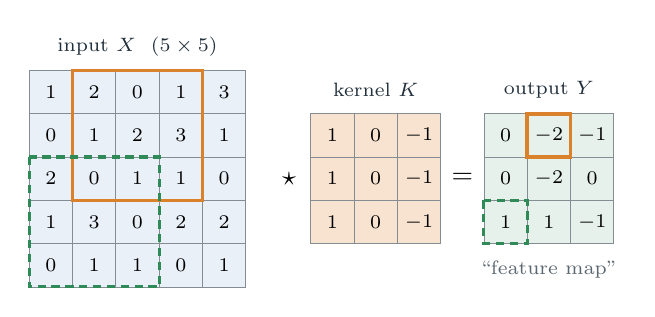
\begin{tikzpicture}[x=5.5mm,y=5.5mm]
  \cellrow{0}{0}{gc,fill=cEmb!10}{1,2,0,1,3}
  \cellrow{0}{1}{gc,fill=cEmb!10}{0,1,2,3,1}
  \cellrow{0}{2}{gc,fill=cEmb!10}{2,0,1,1,0}
  \cellrow{0}{3}{gc,fill=cEmb!10}{1,3,0,2,2}
  \cellrow{0}{4}{gc,fill=cEmb!10}{0,1,1,0,1}
  \draw[cAtt,line width=1.3pt] (0.5,0.5) rectangle (3.5,-2.5);
  \draw[cFfn,line width=1.1pt,densely dashed] (-0.5,-1.5) rectangle (2.5,-4.5);
  \node at (5.5,-2) {$\xcorr$};
  \foreach \r in {1,2,3} {\cellrow{6.5}{\r}{gc,fill=cAtt!22}{1,0,$-1$}}
  \node at (9.5,-2) {$=$};
  \cellrow{10.5}{1}{gc,fill=cFfn!12}{0,$-2$,$-1$}
  \cellrow{10.5}{2}{gc,fill=cFfn!12}{0,$-2$,0}
  \cellrow{10.5}{3}{gc,fill=cFfn!12}{1,1,$-1$}
  \draw[cAtt,line width=1.3pt] (11,-0.5) rectangle (12,-1.5);
  \draw[cFfn,line width=1.1pt,densely dashed] (10,-2.5) rectangle (11,-3.5);
  \node[note,text=cInk] at (2,1.05) {input $X$ \ ($5\times5$)};
  \node[note,text=cInk] at (7.5,0.05) {kernel $K$};
  \node[note,text=cInk] at (11.5,0.05) {output $Y$};
  \node[note] at (11.5,-4.1) {``feature map''};
\end{tikzpicture}

\vspace{1mm}
\raggedright\footnotesize
\textbf{\color{cAtt}Orange window}, $Y_{0,1}$: multiply the kernel entry by entry with the patch
$\bigl[\begin{smallmatrix}2&0&1\\1&2&3\\0&1&1\end{smallmatrix}\bigr]$ and add up:
\[
  Y_{0,1}=(2+1+0)\cdot1+(0+2+1)\cdot0+(1+3+1)\cdot(-1)=3-5=\num{-2}
\]
\textbf{\color{cFfn}Green window}, $Y_{2,0}$: \ $(2+1+0)-(1+0+1)=3-2=\num{1}$.

\vspace{1mm}
This kernel computes ``left column minus right column'': it responds where brightness changes
from left to right. Nine multiplications per output value, the same nine weights everywhere.
\column{0.43\textwidth}
\small
\begin{block}{Definition (one channel, no padding, stride 1)}
\vspace{-2mm}
\[
  Y_{i,j}=b+\sum_{u=0}^{k-1}\sum_{v=0}^{k-1}K_{u,v}\,X_{i+u,\;j+v}
\]
\footnotesize $k$: kernel size; $b$: one bias per kernel. Output size $n-k+1$: here $5-3+1=3$.
\end{block}
\begin{itemize}\footnotesize
  \item The \key{kernel} (or \emph{filter}) is a small array of weights. It is the thing that is learned.
  \item Each output value is a dot product: it is large where the patch looks like the kernel.
  \item An output unit sees only a $k\times k$ patch: \key{local connectivity}. The same kernel
        is used at every position: \key{weight sharing} (slide 8).
\end{itemize}
\begin{block}{A note on the name}
\footnotesize
Mathematicians call this \key{cross-correlation}, written $X\xcorr K$. True convolution $X*K$ flips the
kernel first, $K_{u,v}\to K_{k-1-u,\,k-1-v}$. Deep-learning libraries do not flip.
Since $K$ is learned, the difference is only a relabelling of the weights \cite{14}.
\end{block}
\end{columns}
\end{frame}

% ======================================================================= 4
\begin{frame}{Kernels are feature detectors: Sobel edge filters on a real image}
\centering
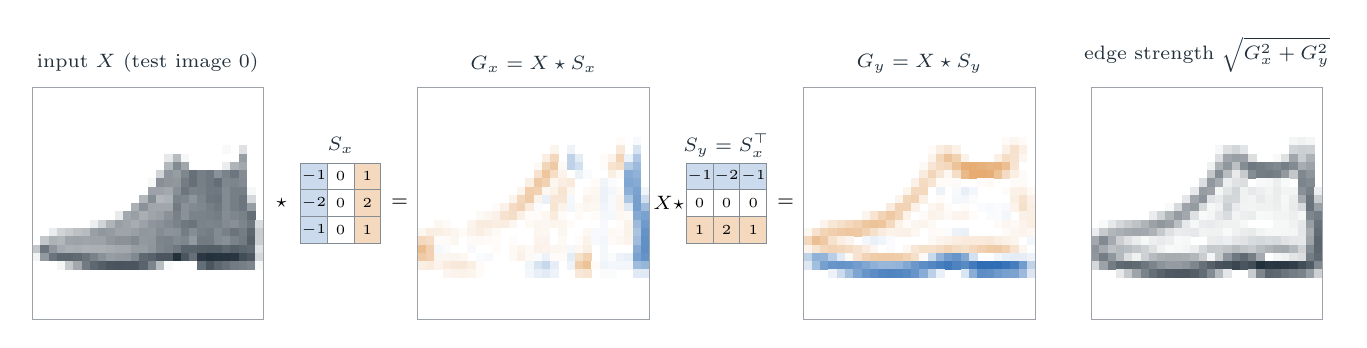
\begin{tikzpicture}[x=1.05mm,y=1.05mm]
  \fill[cInk!3] (23.00,-7.00) rectangle ++(1.04,-1.04);
\fill[cInk!15] (25.00,-7.00) rectangle ++(1.04,-1.04);
\fill[cInk!11] (16.00,-8.00) rectangle ++(1.04,-1.04);
\fill[cInk!33] (17.00,-8.00) rectangle ++(1.04,-1.04);
\fill[cInk!4] (18.00,-8.00) rectangle ++(1.04,-1.04);
\fill[cInk!47] (25.00,-8.00) rectangle ++(1.04,-1.04);
\fill[cInk!35] (16.00,-9.00) rectangle ++(1.04,-1.04);
\fill[cInk!56] (17.00,-9.00) rectangle ++(1.04,-1.04);
\fill[cInk!43] (18.00,-9.00) rectangle ++(1.04,-1.04);
\fill[cInk!9] (23.00,-9.00) rectangle ++(1.04,-1.04);
\fill[cInk!36] (24.00,-9.00) rectangle ++(1.04,-1.04);
\fill[cInk!42] (25.00,-9.00) rectangle ++(1.04,-1.04);
\fill[cInk!21] (15.00,-10.00) rectangle ++(1.04,-1.04);
\fill[cInk!51] (16.00,-10.00) rectangle ++(1.04,-1.04);
\fill[cInk!47] (17.00,-10.00) rectangle ++(1.04,-1.04);
\fill[cInk!58] (18.00,-10.00) rectangle ++(1.04,-1.04);
\fill[cInk!69] (19.00,-10.00) rectangle ++(1.04,-1.04);
\fill[cInk!62] (20.00,-10.00) rectangle ++(1.04,-1.04);
\fill[cInk!65] (21.00,-10.00) rectangle ++(1.04,-1.04);
\fill[cInk!53] (22.00,-10.00) rectangle ++(1.04,-1.04);
\fill[cInk!60] (23.00,-10.00) rectangle ++(1.04,-1.04);
\fill[cInk!66] (24.00,-10.00) rectangle ++(1.04,-1.04);
\fill[cInk!55] (25.00,-10.00) rectangle ++(1.04,-1.04);
\fill[cInk!4] (14.00,-11.00) rectangle ++(1.04,-1.04);
\fill[cInk!54] (15.00,-11.00) rectangle ++(1.04,-1.04);
\fill[cInk!51] (16.00,-11.00) rectangle ++(1.04,-1.04);
\fill[cInk!50] (17.00,-11.00) rectangle ++(1.04,-1.04);
\fill[cInk!63] (18.00,-11.00) rectangle ++(1.04,-1.04);
\fill[cInk!69] (19.00,-11.00) rectangle ++(1.04,-1.04);
\fill[cInk!62] (20.00,-11.00) rectangle ++(1.04,-1.04);
\fill[cInk!65] (21.00,-11.00) rectangle ++(1.04,-1.04);
\fill[cInk!70] (22.00,-11.00) rectangle ++(1.04,-1.04);
\fill[cInk!58] (23.00,-11.00) rectangle ++(1.04,-1.04);
\fill[cInk!59] (24.00,-11.00) rectangle ++(1.04,-1.04);
\fill[cInk!56] (25.00,-11.00) rectangle ++(1.04,-1.04);
\fill[cInk!45] (14.00,-12.00) rectangle ++(2.04,-1.04);
\fill[cInk!42] (16.00,-12.00) rectangle ++(1.04,-1.04);
\fill[cInk!54] (17.00,-12.00) rectangle ++(1.04,-1.04);
\fill[cInk!66] (18.00,-12.00) rectangle ++(1.04,-1.04);
\fill[cInk!60] (19.00,-12.00) rectangle ++(1.04,-1.04);
\fill[cInk!61] (20.00,-12.00) rectangle ++(1.04,-1.04);
\fill[cInk!65] (21.00,-12.00) rectangle ++(2.04,-1.04);
\fill[cInk!56] (23.00,-12.00) rectangle ++(1.04,-1.04);
\fill[cInk!62] (24.00,-12.00) rectangle ++(2.04,-1.04);
\fill[cInk!4] (26.00,-12.00) rectangle ++(1.04,-1.04);
\fill[cInk!35] (13.00,-13.00) rectangle ++(1.04,-1.04);
\fill[cInk!55] (14.00,-13.00) rectangle ++(1.04,-1.04);
\fill[cInk!35] (15.00,-13.00) rectangle ++(1.04,-1.04);
\fill[cInk!37] (16.00,-13.00) rectangle ++(1.04,-1.04);
\fill[cInk!60] (17.00,-13.00) rectangle ++(1.04,-1.04);
\fill[cInk!58] (18.00,-13.00) rectangle ++(1.04,-1.04);
\fill[cInk!51] (19.00,-13.00) rectangle ++(1.04,-1.04);
\fill[cInk!59] (20.00,-13.00) rectangle ++(1.04,-1.04);
\fill[cInk!66] (21.00,-13.00) rectangle ++(1.04,-1.04);
\fill[cInk!67] (22.00,-13.00) rectangle ++(1.04,-1.04);
\fill[cInk!56] (23.00,-13.00) rectangle ++(1.04,-1.04);
\fill[cInk!62] (24.00,-13.00) rectangle ++(1.04,-1.04);
\fill[cInk!66] (25.00,-13.00) rectangle ++(1.04,-1.04);
\fill[cInk!19] (26.00,-13.00) rectangle ++(1.04,-1.04);
\fill[cInk!38] (12.00,-14.00) rectangle ++(1.04,-1.04);
\fill[cInk!53] (13.00,-14.00) rectangle ++(1.04,-1.04);
\fill[cInk!43] (14.00,-14.00) rectangle ++(3.04,-1.04);
\fill[cInk!64] (17.00,-14.00) rectangle ++(1.04,-1.04);
\fill[cInk!53] (18.00,-14.00) rectangle ++(1.04,-1.04);
\fill[cInk!56] (19.00,-14.00) rectangle ++(1.04,-1.04);
\fill[cInk!58] (20.00,-14.00) rectangle ++(1.04,-1.04);
\fill[cInk!62] (21.00,-14.00) rectangle ++(1.04,-1.04);
\fill[cInk!65] (22.00,-14.00) rectangle ++(1.04,-1.04);
\fill[cInk!56] (23.00,-14.00) rectangle ++(1.04,-1.04);
\fill[cInk!62] (24.00,-14.00) rectangle ++(1.04,-1.04);
\fill[cInk!66] (25.00,-14.00) rectangle ++(1.04,-1.04);
\fill[cInk!47] (26.00,-14.00) rectangle ++(1.04,-1.04);
\fill[cInk!10] (10.00,-15.00) rectangle ++(1.04,-1.04);
\fill[cInk!42] (11.00,-15.00) rectangle ++(1.04,-1.04);
\fill[cInk!46] (12.00,-15.00) rectangle ++(1.04,-1.04);
\fill[cInk!39] (13.00,-15.00) rectangle ++(1.04,-1.04);
\fill[cInk!44] (14.00,-15.00) rectangle ++(1.04,-1.04);
\fill[cInk!46] (15.00,-15.00) rectangle ++(1.04,-1.04);
\fill[cInk!53] (16.00,-15.00) rectangle ++(1.04,-1.04);
\fill[cInk!61] (17.00,-15.00) rectangle ++(1.04,-1.04);
\fill[cInk!53] (18.00,-15.00) rectangle ++(1.04,-1.04);
\fill[cInk!60] (19.00,-15.00) rectangle ++(2.04,-1.04);
\fill[cInk!61] (21.00,-15.00) rectangle ++(1.04,-1.04);
\fill[cInk!63] (22.00,-15.00) rectangle ++(1.04,-1.04);
\fill[cInk!55] (23.00,-15.00) rectangle ++(1.04,-1.04);
\fill[cInk!58] (24.00,-15.00) rectangle ++(1.04,-1.04);
\fill[cInk!61] (25.00,-15.00) rectangle ++(1.04,-1.04);
\fill[cInk!70] (26.00,-15.00) rectangle ++(1.04,-1.04);
\fill[cInk!8] (7.00,-16.00) rectangle ++(1.04,-1.04);
\fill[cInk!21] (8.00,-16.00) rectangle ++(1.04,-1.04);
\fill[cInk!36] (9.00,-16.00) rectangle ++(1.04,-1.04);
\fill[cInk!46] (10.00,-16.00) rectangle ++(1.04,-1.04);
\fill[cInk!44] (11.00,-16.00) rectangle ++(1.04,-1.04);
\fill[cInk!40] (12.00,-16.00) rectangle ++(1.04,-1.04);
\fill[cInk!45] (13.00,-16.00) rectangle ++(1.04,-1.04);
\fill[cInk!51] (14.00,-16.00) rectangle ++(1.04,-1.04);
\fill[cInk!53] (15.00,-16.00) rectangle ++(1.04,-1.04);
\fill[cInk!56] (16.00,-16.00) rectangle ++(1.04,-1.04);
\fill[cInk!60] (17.00,-16.00) rectangle ++(1.04,-1.04);
\fill[cInk!65] (18.00,-16.00) rectangle ++(1.04,-1.04);
\fill[cInk!67] (19.00,-16.00) rectangle ++(1.04,-1.04);
\fill[cInk!60] (20.00,-16.00) rectangle ++(1.04,-1.04);
\fill[cInk!59] (21.00,-16.00) rectangle ++(1.04,-1.04);
\fill[cInk!60] (22.00,-16.00) rectangle ++(1.04,-1.04);
\fill[cInk!56] (23.00,-16.00) rectangle ++(1.04,-1.04);
\fill[cInk!54] (24.00,-16.00) rectangle ++(1.04,-1.04);
\fill[cInk!59] (25.00,-16.00) rectangle ++(1.04,-1.04);
\fill[cInk!65] (26.00,-16.00) rectangle ++(1.04,-1.04);
\fill[cInk!17] (27.00,-16.00) rectangle ++(1.04,-1.04);
\fill[cInk!9] (2.00,-17.00) rectangle ++(1.04,-1.04);
\fill[cInk!21] (3.00,-17.00) rectangle ++(1.04,-1.04);
\fill[cInk!25] (4.00,-17.00) rectangle ++(1.04,-1.04);
\fill[cInk!30] (5.00,-17.00) rectangle ++(1.04,-1.04);
\fill[cInk!33] (6.00,-17.00) rectangle ++(1.04,-1.04);
\fill[cInk!46] (7.00,-17.00) rectangle ++(1.04,-1.04);
\fill[cInk!50] (8.00,-17.00) rectangle ++(1.04,-1.04);
\fill[cInk!48] (9.00,-17.00) rectangle ++(1.04,-1.04);
\fill[cInk!44] (10.00,-17.00) rectangle ++(2.04,-1.04);
\fill[cInk!46] (12.00,-17.00) rectangle ++(1.04,-1.04);
\fill[cInk!50] (13.00,-17.00) rectangle ++(1.04,-1.04);
\fill[cInk!49] (14.00,-17.00) rectangle ++(1.04,-1.04);
\fill[cInk!55] (15.00,-17.00) rectangle ++(1.04,-1.04);
\fill[cInk!52] (16.00,-17.00) rectangle ++(1.04,-1.04);
\fill[cInk!53] (17.00,-17.00) rectangle ++(1.04,-1.04);
\fill[cInk!63] (18.00,-17.00) rectangle ++(1.04,-1.04);
\fill[cInk!55] (19.00,-17.00) rectangle ++(1.04,-1.04);
\fill[cInk!61] (20.00,-17.00) rectangle ++(1.04,-1.04);
\fill[cInk!63] (21.00,-17.00) rectangle ++(1.04,-1.04);
\fill[cInk!56] (22.00,-17.00) rectangle ++(1.04,-1.04);
\fill[cInk!61] (23.00,-17.00) rectangle ++(1.04,-1.04);
\fill[cInk!67] (24.00,-17.00) rectangle ++(1.04,-1.04);
\fill[cInk!63] (25.00,-17.00) rectangle ++(1.04,-1.04);
\fill[cInk!74] (26.00,-17.00) rectangle ++(1.04,-1.04);
\fill[cInk!24] (27.00,-17.00) rectangle ++(1.04,-1.04);
\fill[cInk!27] (1.00,-18.00) rectangle ++(1.04,-1.04);
\fill[cInk!37] (2.00,-18.00) rectangle ++(1.04,-1.04);
\fill[cInk!35] (3.00,-18.00) rectangle ++(1.04,-1.04);
\fill[cInk!44] (4.00,-18.00) rectangle ++(1.04,-1.04);
\fill[cInk!45] (5.00,-18.00) rectangle ++(1.04,-1.04);
\fill[cInk!44] (6.00,-18.00) rectangle ++(1.04,-1.04);
\fill[cInk!45] (7.00,-18.00) rectangle ++(2.04,-1.04);
\fill[cInk!50] (9.00,-18.00) rectangle ++(1.04,-1.04);
\fill[cInk!53] (10.00,-18.00) rectangle ++(2.04,-1.04);
\fill[cInk!56] (12.00,-18.00) rectangle ++(1.04,-1.04);
\fill[cInk!49] (13.00,-18.00) rectangle ++(1.04,-1.04);
\fill[cInk!50] (14.00,-18.00) rectangle ++(1.04,-1.04);
\fill[cInk!59] (15.00,-18.00) rectangle ++(1.04,-1.04);
\fill[cInk!60] (16.00,-18.00) rectangle ++(1.04,-1.04);
\fill[cInk!56] (17.00,-18.00) rectangle ++(1.04,-1.04);
\fill[cInk!58] (18.00,-18.00) rectangle ++(1.04,-1.04);
\fill[cInk!49] (19.00,-18.00) rectangle ++(1.04,-1.04);
\fill[cInk!64] (20.00,-18.00) rectangle ++(2.04,-1.04);
\fill[cInk!56] (22.00,-18.00) rectangle ++(1.04,-1.04);
\fill[cInk!54] (23.00,-18.00) rectangle ++(1.04,-1.04);
\fill[cInk!60] (24.00,-18.00) rectangle ++(1.04,-1.04);
\fill[cInk!64] (25.00,-18.00) rectangle ++(1.04,-1.04);
\fill[cInk!77] (26.00,-18.00) rectangle ++(1.04,-1.04);
\fill[cInk!23] (27.00,-18.00) rectangle ++(1.04,-1.04);
\fill[cInk!27] (0.00,-19.00) rectangle ++(1.04,-1.04);
\fill[cInk!66] (1.00,-19.00) rectangle ++(1.04,-1.04);
\fill[cInk!51] (2.00,-19.00) rectangle ++(1.04,-1.04);
\fill[cInk!41] (3.00,-19.00) rectangle ++(1.04,-1.04);
\fill[cInk!38] (4.00,-19.00) rectangle ++(1.04,-1.04);
\fill[cInk!39] (5.00,-19.00) rectangle ++(1.04,-1.04);
\fill[cInk!37] (6.00,-19.00) rectangle ++(1.04,-1.04);
\fill[cInk!38] (7.00,-19.00) rectangle ++(2.04,-1.04);
\fill[cInk!40] (9.00,-19.00) rectangle ++(1.04,-1.04);
\fill[cInk!42] (10.00,-19.00) rectangle ++(2.04,-1.04);
\fill[cInk!47] (12.00,-19.00) rectangle ++(2.04,-1.04);
\fill[cInk!51] (14.00,-19.00) rectangle ++(1.04,-1.04);
\fill[cInk!58] (15.00,-19.00) rectangle ++(1.04,-1.04);
\fill[cInk!61] (16.00,-19.00) rectangle ++(1.04,-1.04);
\fill[cInk!65] (17.00,-19.00) rectangle ++(1.04,-1.04);
\fill[cInk!75] (18.00,-19.00) rectangle ++(2.04,-1.04);
\fill[cInk!77] (20.00,-19.00) rectangle ++(1.04,-1.04);
\fill[cInk!78] (21.00,-19.00) rectangle ++(2.04,-1.04);
\fill[cInk!73] (23.00,-19.00) rectangle ++(1.04,-1.04);
\fill[cInk!77] (24.00,-19.00) rectangle ++(1.04,-1.04);
\fill[cInk!74] (25.00,-19.00) rectangle ++(1.04,-1.04);
\fill[cInk!72] (26.00,-19.00) rectangle ++(1.04,-1.04);
\fill[cInk!14] (27.00,-19.00) rectangle ++(1.04,-1.04);
\fill[cInk!6] (0.00,-20.00) rectangle ++(1.04,-1.04);
\fill[cInk!49] (1.00,-20.00) rectangle ++(1.04,-1.04);
\fill[cInk!67] (2.00,-20.00) rectangle ++(1.04,-1.04);
\fill[cInk!74] (3.00,-20.00) rectangle ++(2.04,-1.04);
\fill[cInk!72] (5.00,-20.00) rectangle ++(1.04,-1.04);
\fill[cInk!67] (6.00,-20.00) rectangle ++(1.04,-1.04);
\fill[cInk!60] (7.00,-20.00) rectangle ++(1.04,-1.04);
\fill[cInk!53] (8.00,-20.00) rectangle ++(1.04,-1.04);
\fill[cInk!47] (9.00,-20.00) rectangle ++(1.04,-1.04);
\fill[cInk!49] (10.00,-20.00) rectangle ++(1.04,-1.04);
\fill[cInk!50] (11.00,-20.00) rectangle ++(1.04,-1.04);
\fill[cInk!57] (12.00,-20.00) rectangle ++(1.04,-1.04);
\fill[cInk!73] (13.00,-20.00) rectangle ++(1.04,-1.04);
\fill[cInk!76] (14.00,-20.00) rectangle ++(1.04,-1.04);
\fill[cInk!82] (15.00,-20.00) rectangle ++(2.04,-1.04);
\fill[cInk!100] (17.00,-20.00) rectangle ++(1.04,-1.04);
\fill[cInk!82] (18.00,-20.00) rectangle ++(1.04,-1.04);
\fill[cInk!69] (19.00,-20.00) rectangle ++(1.04,-1.04);
\fill[cInk!96] (20.00,-20.00) rectangle ++(1.04,-1.04);
\fill[cInk!99] (21.00,-20.00) rectangle ++(1.04,-1.04);
\fill[cInk!98] (22.00,-20.00) rectangle ++(2.04,-1.04);
\fill[cInk!97] (24.00,-20.00) rectangle ++(1.04,-1.04);
\fill[cInk!86] (25.00,-20.00) rectangle ++(1.04,-1.04);
\fill[cInk!81] (26.00,-20.00) rectangle ++(1.04,-1.04);
\fill[cInk!19] (27.00,-20.00) rectangle ++(1.04,-1.04);
\fill[cInk!5] (3.00,-21.00) rectangle ++(1.04,-1.04);
\fill[cInk!26] (4.00,-21.00) rectangle ++(1.04,-1.04);
\fill[cInk!42] (5.00,-21.00) rectangle ++(1.04,-1.04);
\fill[cInk!64] (6.00,-21.00) rectangle ++(1.04,-1.04);
\fill[cInk!73] (7.00,-21.00) rectangle ++(1.04,-1.04);
\fill[cInk!78] (8.00,-21.00) rectangle ++(1.04,-1.04);
\fill[cInk!82] (9.00,-21.00) rectangle ++(1.04,-1.04);
\fill[cInk!83] (10.00,-21.00) rectangle ++(1.04,-1.04);
\fill[cInk!82] (11.00,-21.00) rectangle ++(2.04,-1.04);
\fill[cInk!75] (13.00,-21.00) rectangle ++(1.04,-1.04);
\fill[cInk!59] (14.00,-21.00) rectangle ++(1.04,-1.04);
\fill[cInk!32] (15.00,-21.00) rectangle ++(1.04,-1.04);
\fill[cInk!3] (16.00,-21.00) rectangle ++(1.04,-1.04);
\fill[cInk!70] (20.00,-21.00) rectangle ++(1.04,-1.04);
\fill[cInk!82] (21.00,-21.00) rectangle ++(1.04,-1.04);
\fill[cInk!74] (22.00,-21.00) rectangle ++(1.04,-1.04);
\fill[cInk!69] (23.00,-21.00) rectangle ++(1.04,-1.04);
\fill[cInk!64] (24.00,-21.00) rectangle ++(1.04,-1.04);
\fill[cInk!62] (25.00,-21.00) rectangle ++(1.04,-1.04);
\fill[cInk!59] (26.00,-21.00) rectangle ++(1.04,-1.04);
\fill[cInk!4] (27.00,-21.00) rectangle ++(1.04,-1.04);
\draw[cInk!45,line width=0.3pt] (0.00,0.00) rectangle ++(28,-28);

  \node[note,text=cInk,anchor=south] at (14,0.6) {input $X$ (test image 0)};
  \begin{scope}[xshift=49mm] \fill[cAtt!3] (24.00,-6.00) rectangle ++(1.04,-1.04);
\fill[cEmb!4] (26.00,-6.00) rectangle ++(1.04,-1.04);
\fill[cAtt!8] (16.00,-7.00) rectangle ++(1.04,-1.04);
\fill[cEmb!8] (18.00,-7.00) rectangle ++(1.04,-1.04);
\fill[cAtt!18] (24.00,-7.00) rectangle ++(1.04,-1.04);
\fill[cEmb!19] (26.00,-7.00) rectangle ++(1.04,-1.04);
\fill[cAtt!14] (15.00,-8.00) rectangle ++(1.04,-1.04);
\fill[cAtt!31] (16.00,-8.00) rectangle ++(1.04,-1.04);
\fill[cEmb!31] (18.00,-8.00) rectangle ++(1.04,-1.04);
\fill[cEmb!13] (19.00,-8.00) rectangle ++(1.04,-1.04);
\fill[cAtt!3] (22.00,-8.00) rectangle ++(1.04,-1.04);
\fill[cAtt!9] (23.00,-8.00) rectangle ++(1.04,-1.04);
\fill[cAtt!35] (24.00,-8.00) rectangle ++(1.04,-1.04);
\fill[cEmb!9] (25.00,-8.00) rectangle ++(1.04,-1.04);
\fill[cEmb!38] (26.00,-8.00) rectangle ++(1.04,-1.04);
\fill[cAtt!5] (14.00,-9.00) rectangle ++(1.04,-1.04);
\fill[cAtt!33] (15.00,-9.00) rectangle ++(1.04,-1.04);
\fill[cAtt!43] (16.00,-9.00) rectangle ++(1.04,-1.04);
\fill[cAtt!5] (17.00,-9.00) rectangle ++(1.04,-1.04);
\fill[cEmb!31] (18.00,-9.00) rectangle ++(1.04,-1.04);
\fill[cEmb!22] (19.00,-9.00) rectangle ++(1.04,-1.04);
\fill[cAtt!3] (22.00,-9.00) rectangle ++(1.04,-1.04);
\fill[cAtt!22] (23.00,-9.00) rectangle ++(1.04,-1.04);
\fill[cAtt!27] (24.00,-9.00) rectangle ++(1.04,-1.04);
\fill[cEmb!35] (25.00,-9.00) rectangle ++(1.04,-1.04);
\fill[cEmb!47] (26.00,-9.00) rectangle ++(1.04,-1.04);
\fill[cAtt!23] (14.00,-10.00) rectangle ++(1.04,-1.04);
\fill[cAtt!46] (15.00,-10.00) rectangle ++(1.04,-1.04);
\fill[cAtt!27] (16.00,-10.00) rectangle ++(1.04,-1.04);
\fill[cAtt!9] (17.00,-10.00) rectangle ++(1.04,-1.04);
\fill[cEmb!9] (19.00,-10.00) rectangle ++(1.04,-1.04);
\fill[cEmb!3] (20.00,-10.00) rectangle ++(1.04,-1.04);
\fill[cAtt!13] (23.00,-10.00) rectangle ++(1.04,-1.04);
\fill[cAtt!5] (24.00,-10.00) rectangle ++(1.04,-1.04);
\fill[cEmb!58] (25.00,-10.00) rectangle ++(1.04,-1.04);
\fill[cEmb!53] (26.00,-10.00) rectangle ++(1.04,-1.04);
\fill[cAtt!13] (13.00,-11.00) rectangle ++(1.04,-1.04);
\fill[cAtt!43] (14.00,-11.00) rectangle ++(1.04,-1.04);
\fill[cAtt!36] (15.00,-11.00) rectangle ++(1.04,-1.04);
\fill[cAtt!7] (16.00,-11.00) rectangle ++(1.04,-1.04);
\fill[cAtt!14] (17.00,-11.00) rectangle ++(1.04,-1.04);
\fill[cAtt!17] (18.00,-11.00) rectangle ++(1.04,-1.04);
\fill[cAtt!3] (21.00,-11.00) rectangle ++(1.04,-1.04);
\fill[cEmb!7] (22.00,-11.00) rectangle ++(1.04,-1.04);
\fill[cEmb!3] (23.00,-11.00) rectangle ++(1.04,-1.04);
\fill[cEmb!61] (25.00,-11.00) rectangle ++(1.04,-1.04);
\fill[cEmb!58] (26.00,-11.00) rectangle ++(1.04,-1.04);
\fill[cAtt!8] (12.00,-12.00) rectangle ++(1.04,-1.04);
\fill[cAtt!38] (13.00,-12.00) rectangle ++(1.04,-1.04);
\fill[cAtt!36] (14.00,-12.00) rectangle ++(1.04,-1.04);
\fill[cAtt!6] (15.00,-12.00) rectangle ++(1.04,-1.04);
\fill[cAtt!10] (16.00,-12.00) rectangle ++(1.04,-1.04);
\fill[cAtt!21] (17.00,-12.00) rectangle ++(1.04,-1.04);
\fill[cAtt!6] (18.00,-12.00) rectangle ++(1.04,-1.04);
\fill[cAtt!5] (20.00,-12.00) rectangle ++(1.04,-1.04);
\fill[cAtt!6] (21.00,-12.00) rectangle ++(1.04,-1.04);
\fill[cEmb!9] (22.00,-12.00) rectangle ++(1.04,-1.04);
\fill[cEmb!6] (23.00,-12.00) rectangle ++(1.04,-1.04);
\fill[cAtt!5] (24.00,-12.00) rectangle ++(1.04,-1.04);
\fill[cEmb!55] (25.00,-12.00) rectangle ++(1.04,-1.04);
\fill[cEmb!63] (26.00,-12.00) rectangle ++(1.04,-1.04);
\fill[cEmb!7] (27.00,-12.00) rectangle ++(1.04,-1.04);
\fill[cAtt!9] (11.00,-13.00) rectangle ++(1.04,-1.04);
\fill[cAtt!31] (12.00,-13.00) rectangle ++(1.04,-1.04);
\fill[cAtt!40] (13.00,-13.00) rectangle ++(1.04,-1.04);
\fill[cAtt!9] (14.00,-13.00) rectangle ++(1.04,-1.04);
\fill[cEmb!10] (15.00,-13.00) rectangle ++(1.04,-1.04);
\fill[cAtt!20] (16.00,-13.00) rectangle ++(2.04,-1.04);
\fill[cEmb!5] (18.00,-13.00) rectangle ++(1.04,-1.04);
\fill[cAtt!10] (20.00,-13.00) rectangle ++(1.04,-1.04);
\fill[cAtt!7] (21.00,-13.00) rectangle ++(1.04,-1.04);
\fill[cEmb!9] (22.00,-13.00) rectangle ++(1.04,-1.04);
\fill[cEmb!4] (23.00,-13.00) rectangle ++(1.04,-1.04);
\fill[cAtt!9] (24.00,-13.00) rectangle ++(1.04,-1.04);
\fill[cEmb!40] (25.00,-13.00) rectangle ++(1.04,-1.04);
\fill[cEmb!66] (26.00,-13.00) rectangle ++(1.04,-1.04);
\fill[cEmb!22] (27.00,-13.00) rectangle ++(1.04,-1.04);
\fill[cAtt!3] (9.00,-14.00) rectangle ++(1.04,-1.04);
\fill[cAtt!11] (10.00,-14.00) rectangle ++(1.04,-1.04);
\fill[cAtt!28] (11.00,-14.00) rectangle ++(1.04,-1.04);
\fill[cAtt!35] (12.00,-14.00) rectangle ++(1.04,-1.04);
\fill[cAtt!16] (13.00,-14.00) rectangle ++(1.04,-1.04);
\fill[cEmb!3] (14.00,-14.00) rectangle ++(1.04,-1.04);
\fill[cAtt!21] (16.00,-14.00) rectangle ++(1.04,-1.04);
\fill[cAtt!10] (17.00,-14.00) rectangle ++(1.04,-1.04);
\fill[cEmb!6] (18.00,-14.00) rectangle ++(1.04,-1.04);
\fill[cAtt!5] (19.00,-14.00) rectangle ++(1.04,-1.04);
\fill[cAtt!7] (20.00,-14.00) rectangle ++(1.04,-1.04);
\fill[cAtt!6] (21.00,-14.00) rectangle ++(1.04,-1.04);
\fill[cEmb!7] (22.00,-14.00) rectangle ++(1.04,-1.04);
\fill[cEmb!4] (23.00,-14.00) rectangle ++(1.04,-1.04);
\fill[cAtt!9] (24.00,-14.00) rectangle ++(1.04,-1.04);
\fill[cEmb!16] (25.00,-14.00) rectangle ++(1.04,-1.04);
\fill[cEmb!66] (26.00,-14.00) rectangle ++(1.04,-1.04);
\fill[cEmb!46] (27.00,-14.00) rectangle ++(1.04,-1.04);
\fill[cAtt!5] (7.00,-15.00) rectangle ++(1.04,-1.04);
\fill[cAtt!7] (8.00,-15.00) rectangle ++(1.04,-1.04);
\fill[cAtt!11] (9.00,-15.00) rectangle ++(1.04,-1.04);
\fill[cAtt!23] (10.00,-15.00) rectangle ++(1.04,-1.04);
\fill[cAtt!26] (11.00,-15.00) rectangle ++(1.04,-1.04);
\fill[cAtt!12] (12.00,-15.00) rectangle ++(1.04,-1.04);
\fill[cAtt!3] (13.00,-15.00) rectangle ++(2.04,-1.04);
\fill[cAtt!6] (15.00,-15.00) rectangle ++(1.04,-1.04);
\fill[cAtt!15] (16.00,-15.00) rectangle ++(1.04,-1.04);
\fill[cAtt!4] (17.00,-15.00) rectangle ++(1.04,-1.04);
\fill[cAtt!4] (19.00,-15.00) rectangle ++(1.04,-1.04);
\fill[cAtt!3] (21.00,-15.00) rectangle ++(1.04,-1.04);
\fill[cEmb!5] (22.00,-15.00) rectangle ++(2.04,-1.04);
\fill[cAtt!6] (24.00,-15.00) rectangle ++(1.04,-1.04);
\fill[cAtt!5] (25.00,-15.00) rectangle ++(1.04,-1.04);
\fill[cEmb!59] (26.00,-15.00) rectangle ++(1.04,-1.04);
\fill[cEmb!64] (27.00,-15.00) rectangle ++(1.04,-1.04);
\fill[cAtt!6] (2.00,-16.00) rectangle ++(1.04,-1.04);
\fill[cAtt!4] (3.00,-16.00) rectangle ++(1.04,-1.04);
\fill[cAtt!8] (6.00,-16.00) rectangle ++(1.04,-1.04);
\fill[cAtt!15] (7.00,-16.00) rectangle ++(2.04,-1.04);
\fill[cAtt!14] (9.00,-16.00) rectangle ++(2.04,-1.04);
\fill[cAtt!7] (11.00,-16.00) rectangle ++(1.04,-1.04);
\fill[cAtt!5] (13.00,-16.00) rectangle ++(1.04,-1.04);
\fill[cAtt!7] (14.00,-16.00) rectangle ++(1.04,-1.04);
\fill[cAtt!6] (15.00,-16.00) rectangle ++(1.04,-1.04);
\fill[cAtt!8] (16.00,-16.00) rectangle ++(1.04,-1.04);
\fill[cAtt!7] (17.00,-16.00) rectangle ++(1.04,-1.04);
\fill[cAtt!3] (18.00,-16.00) rectangle ++(1.04,-1.04);
\fill[cEmb!4] (22.00,-16.00) rectangle ++(1.04,-1.04);
\fill[cAtt!3] (24.00,-16.00) rectangle ++(1.04,-1.04);
\fill[cAtt!10] (25.00,-16.00) rectangle ++(1.04,-1.04);
\fill[cEmb!47] (26.00,-16.00) rectangle ++(1.04,-1.04);
\fill[cEmb!69] (27.00,-16.00) rectangle ++(1.04,-1.04);
\fill[cAtt!7] (0.00,-17.00) rectangle ++(1.04,-1.04);
\fill[cAtt!14] (1.00,-17.00) rectangle ++(1.04,-1.04);
\fill[cAtt!13] (2.00,-17.00) rectangle ++(1.04,-1.04);
\fill[cAtt!10] (3.00,-17.00) rectangle ++(1.04,-1.04);
\fill[cAtt!7] (4.00,-17.00) rectangle ++(1.04,-1.04);
\fill[cAtt!4] (5.00,-17.00) rectangle ++(1.04,-1.04);
\fill[cAtt!10] (6.00,-17.00) rectangle ++(1.04,-1.04);
\fill[cAtt!14] (7.00,-17.00) rectangle ++(1.04,-1.04);
\fill[cAtt!9] (8.00,-17.00) rectangle ++(1.04,-1.04);
\fill[cAtt!5] (9.00,-17.00) rectangle ++(1.04,-1.04);
\fill[cAtt!7] (14.00,-17.00) rectangle ++(1.04,-1.04);
\fill[cAtt!6] (15.00,-17.00) rectangle ++(1.04,-1.04);
\fill[cAtt!7] (17.00,-17.00) rectangle ++(1.04,-1.04);
\fill[cAtt!6] (20.00,-17.00) rectangle ++(1.04,-1.04);
\fill[cEmb!4] (21.00,-17.00) rectangle ++(2.04,-1.04);
\fill[cAtt!5] (23.00,-17.00) rectangle ++(1.04,-1.04);
\fill[cAtt!4] (24.00,-17.00) rectangle ++(1.04,-1.04);
\fill[cAtt!10] (25.00,-17.00) rectangle ++(1.04,-1.04);
\fill[cEmb!41] (26.00,-17.00) rectangle ++(1.04,-1.04);
\fill[cEmb!74] (27.00,-17.00) rectangle ++(1.04,-1.04);
\fill[cAtt!30] (0.00,-18.00) rectangle ++(1.04,-1.04);
\fill[cAtt!27] (1.00,-18.00) rectangle ++(1.04,-1.04);
\fill[cAtt!3] (2.00,-18.00) rectangle ++(1.04,-1.04);
\fill[cAtt!4] (3.00,-18.00) rectangle ++(1.04,-1.04);
\fill[cAtt!7] (4.00,-18.00) rectangle ++(1.04,-1.04);
\fill[cAtt!4] (6.00,-18.00) rectangle ++(1.04,-1.04);
\fill[cAtt!5] (7.00,-18.00) rectangle ++(1.04,-1.04);
\fill[cAtt!4] (8.00,-18.00) rectangle ++(1.04,-1.04);
\fill[cAtt!3] (9.00,-18.00) rectangle ++(1.04,-1.04);
\fill[cAtt!3] (11.00,-18.00) rectangle ++(1.04,-1.04);
\fill[cAtt!9] (14.00,-18.00) rectangle ++(2.04,-1.04);
\fill[cAtt!5] (17.00,-18.00) rectangle ++(1.04,-1.04);
\fill[cAtt!3] (19.00,-18.00) rectangle ++(1.04,-1.04);
\fill[cAtt!10] (20.00,-18.00) rectangle ++(1.04,-1.04);
\fill[cEmb!4] (21.00,-18.00) rectangle ++(1.04,-1.04);
\fill[cEmb!6] (22.00,-18.00) rectangle ++(1.04,-1.04);
\fill[cAtt!4] (23.00,-18.00) rectangle ++(1.04,-1.04);
\fill[cAtt!6] (24.00,-18.00) rectangle ++(1.04,-1.04);
\fill[cAtt!9] (25.00,-18.00) rectangle ++(1.04,-1.04);
\fill[cEmb!46] (26.00,-18.00) rectangle ++(1.04,-1.04);
\fill[cEmb!76] (27.00,-18.00) rectangle ++(1.04,-1.04);
\fill[cAtt!53] (0.00,-19.00) rectangle ++(1.04,-1.04);
\fill[cAtt!37] (1.00,-19.00) rectangle ++(1.04,-1.04);
\fill[cEmb!5] (2.00,-19.00) rectangle ++(1.04,-1.04);
\fill[cEmb!3] (3.00,-19.00) rectangle ++(1.04,-1.04);
\fill[cEmb!4] (6.00,-19.00) rectangle ++(1.04,-1.04);
\fill[cAtt!3] (9.00,-19.00) rectangle ++(1.04,-1.04);
\fill[cAtt!5] (11.00,-19.00) rectangle ++(1.04,-1.04);
\fill[cAtt!8] (12.00,-19.00) rectangle ++(1.04,-1.04);
\fill[cAtt!5] (13.00,-19.00) rectangle ++(1.04,-1.04);
\fill[cAtt!11] (14.00,-19.00) rectangle ++(1.04,-1.04);
\fill[cAtt!9] (15.00,-19.00) rectangle ++(1.04,-1.04);
\fill[cAtt!7] (16.00,-19.00) rectangle ++(1.04,-1.04);
\fill[cAtt!6] (17.00,-19.00) rectangle ++(1.04,-1.04);
\fill[cEmb!5] (18.00,-19.00) rectangle ++(1.04,-1.04);
\fill[cAtt!6] (19.00,-19.00) rectangle ++(1.04,-1.04);
\fill[cAtt!13] (20.00,-19.00) rectangle ++(1.04,-1.04);
\fill[cEmb!5] (22.00,-19.00) rectangle ++(1.04,-1.04);
\fill[cEmb!58] (26.00,-19.00) rectangle ++(1.04,-1.04);
\fill[cEmb!77] (27.00,-19.00) rectangle ++(1.04,-1.04);
\fill[cAtt!42] (0.00,-20.00) rectangle ++(1.04,-1.04);
\fill[cAtt!37] (1.00,-20.00) rectangle ++(1.04,-1.04);
\fill[cAtt!7] (2.00,-20.00) rectangle ++(2.04,-1.04);
\fill[cAtt!8] (4.00,-20.00) rectangle ++(1.04,-1.04);
\fill[cAtt!6] (5.00,-20.00) rectangle ++(1.04,-1.04);
\fill[cEmb!3] (7.00,-20.00) rectangle ++(1.04,-1.04);
\fill[cEmb!4] (8.00,-20.00) rectangle ++(1.04,-1.04);
\fill[cAtt!5] (11.00,-20.00) rectangle ++(1.04,-1.04);
\fill[cAtt!11] (12.00,-20.00) rectangle ++(1.04,-1.04);
\fill[cAtt!5] (13.00,-20.00) rectangle ++(1.04,-1.04);
\fill[cEmb!3] (14.00,-20.00) rectangle ++(1.04,-1.04);
\fill[cEmb!9] (15.00,-20.00) rectangle ++(1.04,-1.04);
\fill[cAtt!3] (16.00,-20.00) rectangle ++(2.04,-1.04);
\fill[cEmb!13] (18.00,-20.00) rectangle ++(1.04,-1.04);
\fill[cAtt!25] (19.00,-20.00) rectangle ++(1.04,-1.04);
\fill[cAtt!36] (20.00,-20.00) rectangle ++(1.04,-1.04);
\fill[cEmb!5] (22.00,-20.00) rectangle ++(1.04,-1.04);
\fill[cEmb!3] (23.00,-20.00) rectangle ++(1.04,-1.04);
\fill[cEmb!8] (24.00,-20.00) rectangle ++(1.04,-1.04);
\fill[cEmb!11] (25.00,-20.00) rectangle ++(1.04,-1.04);
\fill[cEmb!64] (26.00,-20.00) rectangle ++(1.04,-1.04);
\fill[cEmb!74] (27.00,-20.00) rectangle ++(1.04,-1.04);
\fill[cAtt!13] (0.00,-21.00) rectangle ++(1.04,-1.04);
\fill[cAtt!15] (1.00,-21.00) rectangle ++(1.04,-1.04);
\fill[cAtt!9] (2.00,-21.00) rectangle ++(1.04,-1.04);
\fill[cAtt!15] (3.00,-21.00) rectangle ++(1.04,-1.04);
\fill[cAtt!18] (4.00,-21.00) rectangle ++(2.04,-1.04);
\fill[cAtt!13] (6.00,-21.00) rectangle ++(1.04,-1.04);
\fill[cAtt!3] (7.00,-21.00) rectangle ++(1.04,-1.04);
\fill[cEmb!7] (13.00,-21.00) rectangle ++(1.04,-1.04);
\fill[cEmb!19] (14.00,-21.00) rectangle ++(1.04,-1.04);
\fill[cEmb!27] (15.00,-21.00) rectangle ++(1.04,-1.04);
\fill[cEmb!12] (16.00,-21.00) rectangle ++(1.04,-1.04);
\fill[cEmb!8] (18.00,-21.00) rectangle ++(1.04,-1.04);
\fill[cAtt!39] (19.00,-21.00) rectangle ++(1.04,-1.04);
\fill[cAtt!49] (20.00,-21.00) rectangle ++(1.04,-1.04);
\fill[cAtt!3] (21.00,-21.00) rectangle ++(1.04,-1.04);
\fill[cEmb!7] (22.00,-21.00) rectangle ++(1.04,-1.04);
\fill[cEmb!6] (23.00,-21.00) rectangle ++(3.04,-1.04);
\fill[cEmb!46] (26.00,-21.00) rectangle ++(1.04,-1.04);
\fill[cEmb!51] (27.00,-21.00) rectangle ++(1.04,-1.04);
\fill[cAtt!7] (3.00,-22.00) rectangle ++(1.04,-1.04);
\fill[cAtt!9] (4.00,-22.00) rectangle ++(1.04,-1.04);
\fill[cAtt!10] (5.00,-22.00) rectangle ++(1.04,-1.04);
\fill[cAtt!8] (6.00,-22.00) rectangle ++(1.04,-1.04);
\fill[cAtt!3] (7.00,-22.00) rectangle ++(1.04,-1.04);
\fill[cEmb!6] (13.00,-22.00) rectangle ++(1.04,-1.04);
\fill[cEmb!11] (14.00,-22.00) rectangle ++(1.04,-1.04);
\fill[cEmb!14] (15.00,-22.00) rectangle ++(1.04,-1.04);
\fill[cEmb!8] (16.00,-22.00) rectangle ++(1.04,-1.04);
\fill[cAtt!18] (19.00,-22.00) rectangle ++(1.04,-1.04);
\fill[cAtt!21] (20.00,-22.00) rectangle ++(1.04,-1.04);
\fill[cEmb!3] (22.00,-22.00) rectangle ++(2.04,-1.04);
\fill[cEmb!15] (26.00,-22.00) rectangle ++(2.04,-1.04);
\draw[cInk!45,line width=0.3pt] (0.00,0.00) rectangle ++(28,-28);

    \node[note,text=cInk,anchor=south] at (14,0.6) {$G_x=X\xcorr S_x$}; \end{scope}
  \begin{scope}[xshift=98mm] \fill[cAtt!4] (24.00,-6.00) rectangle ++(1.04,-1.04);
\fill[cAtt!7] (25.00,-6.00) rectangle ++(1.04,-1.04);
\fill[cAtt!4] (26.00,-6.00) rectangle ++(1.04,-1.04);
\fill[cAtt!3] (15.00,-7.00) rectangle ++(1.04,-1.04);
\fill[cAtt!14] (16.00,-7.00) rectangle ++(1.04,-1.04);
\fill[cAtt!20] (17.00,-7.00) rectangle ++(1.04,-1.04);
\fill[cAtt!11] (18.00,-7.00) rectangle ++(1.04,-1.04);
\fill[cAtt!12] (24.00,-7.00) rectangle ++(1.04,-1.04);
\fill[cAtt!24] (25.00,-7.00) rectangle ++(1.04,-1.04);
\fill[cAtt!12] (26.00,-7.00) rectangle ++(1.04,-1.04);
\fill[cAtt!9] (15.00,-8.00) rectangle ++(1.04,-1.04);
\fill[cAtt!32] (16.00,-8.00) rectangle ++(1.04,-1.04);
\fill[cAtt!48] (17.00,-8.00) rectangle ++(1.04,-1.04);
\fill[cAtt!36] (18.00,-8.00) rectangle ++(1.04,-1.04);
\fill[cAtt!10] (19.00,-8.00) rectangle ++(1.04,-1.04);
\fill[cAtt!12] (23.00,-8.00) rectangle ++(1.04,-1.04);
\fill[cAtt!27] (24.00,-8.00) rectangle ++(1.04,-1.04);
\fill[cAtt!23] (25.00,-8.00) rectangle ++(1.04,-1.04);
\fill[cAtt!7] (26.00,-8.00) rectangle ++(1.04,-1.04);
\fill[cAtt!5] (14.00,-9.00) rectangle ++(1.04,-1.04);
\fill[cAtt!20] (15.00,-9.00) rectangle ++(1.04,-1.04);
\fill[cAtt!29] (16.00,-9.00) rectangle ++(1.04,-1.04);
\fill[cAtt!31] (17.00,-9.00) rectangle ++(1.04,-1.04);
\fill[cAtt!48] (18.00,-9.00) rectangle ++(1.04,-1.04);
\fill[cAtt!64] (19.00,-9.00) rectangle ++(1.04,-1.04);
\fill[cAtt!65] (20.00,-9.00) rectangle ++(1.04,-1.04);
\fill[cAtt!62] (21.00,-9.00) rectangle ++(1.04,-1.04);
\fill[cAtt!59] (22.00,-9.00) rectangle ++(1.04,-1.04);
\fill[cAtt!61] (23.00,-9.00) rectangle ++(1.04,-1.04);
\fill[cAtt!51] (24.00,-9.00) rectangle ++(1.04,-1.04);
\fill[cAtt!21] (25.00,-9.00) rectangle ++(1.04,-1.04);
\fill[cAtt!16] (14.00,-10.00) rectangle ++(1.04,-1.04);
\fill[cAtt!33] (15.00,-10.00) rectangle ++(1.04,-1.04);
\fill[cAtt!20] (16.00,-10.00) rectangle ++(1.04,-1.04);
\fill[cAtt!6] (17.00,-10.00) rectangle ++(1.04,-1.04);
\fill[cAtt!26] (18.00,-10.00) rectangle ++(1.04,-1.04);
\fill[cAtt!56] (19.00,-10.00) rectangle ++(1.04,-1.04);
\fill[cAtt!66] (20.00,-10.00) rectangle ++(1.04,-1.04);
\fill[cAtt!67] (21.00,-10.00) rectangle ++(1.04,-1.04);
\fill[cAtt!65] (22.00,-10.00) rectangle ++(1.04,-1.04);
\fill[cAtt!49] (23.00,-10.00) rectangle ++(1.04,-1.04);
\fill[cAtt!28] (24.00,-10.00) rectangle ++(1.04,-1.04);
\fill[cAtt!13] (25.00,-10.00) rectangle ++(1.04,-1.04);
\fill[cAtt!4] (26.00,-10.00) rectangle ++(1.04,-1.04);
\fill[cAtt!11] (13.00,-11.00) rectangle ++(1.04,-1.04);
\fill[cAtt!29] (14.00,-11.00) rectangle ++(1.04,-1.04);
\fill[cAtt!21] (15.00,-11.00) rectangle ++(1.04,-1.04);
\fill[cAtt!3] (16.00,-11.00) rectangle ++(2.04,-1.04);
\fill[cAtt!4] (18.00,-11.00) rectangle ++(1.04,-1.04);
\fill[cAtt!3] (21.00,-11.00) rectangle ++(1.04,-1.04);
\fill[cAtt!5] (22.00,-11.00) rectangle ++(1.04,-1.04);
\fill[cAtt!4] (25.00,-11.00) rectangle ++(2.04,-1.04);
\fill[cAtt!8] (12.00,-12.00) rectangle ++(1.04,-1.04);
\fill[cAtt!30] (13.00,-12.00) rectangle ++(2.04,-1.04);
\fill[cEmb!9] (16.00,-12.00) rectangle ++(1.04,-1.04);
\fill[cEmb!4] (18.00,-12.00) rectangle ++(1.04,-1.04);
\fill[cEmb!11] (19.00,-12.00) rectangle ++(1.04,-1.04);
\fill[cEmb!6] (20.00,-12.00) rectangle ++(1.04,-1.04);
\fill[cAtt!3] (24.00,-12.00) rectangle ++(1.04,-1.04);
\fill[cAtt!11] (25.00,-12.00) rectangle ++(1.04,-1.04);
\fill[cAtt!12] (26.00,-12.00) rectangle ++(1.04,-1.04);
\fill[cAtt!5] (27.00,-12.00) rectangle ++(1.04,-1.04);
\fill[cAtt!9] (11.00,-13.00) rectangle ++(1.04,-1.04);
\fill[cAtt!33] (12.00,-13.00) rectangle ++(1.04,-1.04);
\fill[cAtt!36] (13.00,-13.00) rectangle ++(1.04,-1.04);
\fill[cAtt!12] (14.00,-13.00) rectangle ++(1.04,-1.04);
\fill[cAtt!3] (16.00,-13.00) rectangle ++(1.04,-1.04);
\fill[cEmb!5] (18.00,-13.00) rectangle ++(1.04,-1.04);
\fill[cEmb!6] (19.00,-13.00) rectangle ++(1.04,-1.04);
\fill[cEmb!3] (20.00,-13.00) rectangle ++(1.04,-1.04);
\fill[cAtt!13] (25.00,-13.00) rectangle ++(1.04,-1.04);
\fill[cAtt!23] (26.00,-13.00) rectangle ++(1.04,-1.04);
\fill[cAtt!11] (27.00,-13.00) rectangle ++(1.04,-1.04);
\fill[cAtt!15] (10.00,-14.00) rectangle ++(1.04,-1.04);
\fill[cAtt!35] (11.00,-14.00) rectangle ++(2.04,-1.04);
\fill[cAtt!11] (13.00,-14.00) rectangle ++(1.04,-1.04);
\fill[cAtt!7] (15.00,-14.00) rectangle ++(1.04,-1.04);
\fill[cAtt!11] (16.00,-14.00) rectangle ++(1.04,-1.04);
\fill[cAtt!3] (17.00,-14.00) rectangle ++(1.04,-1.04);
\fill[cAtt!3] (19.00,-14.00) rectangle ++(1.04,-1.04);
\fill[cEmb!3] (21.00,-14.00) rectangle ++(1.04,-1.04);
\fill[cEmb!4] (22.00,-14.00) rectangle ++(1.04,-1.04);
\fill[cEmb!3] (23.00,-14.00) rectangle ++(1.04,-1.04);
\fill[cEmb!4] (24.00,-14.00) rectangle ++(1.04,-1.04);
\fill[cAtt!9] (25.00,-14.00) rectangle ++(1.04,-1.04);
\fill[cAtt!25] (26.00,-14.00) rectangle ++(1.04,-1.04);
\fill[cAtt!13] (27.00,-14.00) rectangle ++(1.04,-1.04);
\fill[cAtt!8] (7.00,-15.00) rectangle ++(1.04,-1.04);
\fill[cAtt!21] (8.00,-15.00) rectangle ++(1.04,-1.04);
\fill[cAtt!35] (9.00,-15.00) rectangle ++(1.04,-1.04);
\fill[cAtt!43] (10.00,-15.00) rectangle ++(1.04,-1.04);
\fill[cAtt!34] (11.00,-15.00) rectangle ++(1.04,-1.04);
\fill[cAtt!10] (12.00,-15.00) rectangle ++(1.04,-1.04);
\fill[cAtt!4] (14.00,-15.00) rectangle ++(1.04,-1.04);
\fill[cAtt!10] (15.00,-15.00) rectangle ++(1.04,-1.04);
\fill[cAtt!8] (16.00,-15.00) rectangle ++(1.04,-1.04);
\fill[cAtt!5] (17.00,-15.00) rectangle ++(1.04,-1.04);
\fill[cAtt!8] (18.00,-15.00) rectangle ++(1.04,-1.04);
\fill[cAtt!9] (19.00,-15.00) rectangle ++(1.04,-1.04);
\fill[cAtt!3] (20.00,-15.00) rectangle ++(1.04,-1.04);
\fill[cEmb!3] (22.00,-15.00) rectangle ++(2.04,-1.04);
\fill[cEmb!6] (24.00,-15.00) rectangle ++(1.04,-1.04);
\fill[cAtt!12] (26.00,-15.00) rectangle ++(1.04,-1.04);
\fill[cAtt!13] (27.00,-15.00) rectangle ++(1.04,-1.04);
\fill[cAtt!9] (2.00,-16.00) rectangle ++(1.04,-1.04);
\fill[cAtt!19] (3.00,-16.00) rectangle ++(1.04,-1.04);
\fill[cAtt!25] (4.00,-16.00) rectangle ++(1.04,-1.04);
\fill[cAtt!30] (5.00,-16.00) rectangle ++(1.04,-1.04);
\fill[cAtt!36] (6.00,-16.00) rectangle ++(1.04,-1.04);
\fill[cAtt!45] (7.00,-16.00) rectangle ++(1.04,-1.04);
\fill[cAtt!49] (8.00,-16.00) rectangle ++(1.04,-1.04);
\fill[cAtt!46] (9.00,-16.00) rectangle ++(1.04,-1.04);
\fill[cAtt!30] (10.00,-16.00) rectangle ++(1.04,-1.04);
\fill[cAtt!10] (11.00,-16.00) rectangle ++(1.04,-1.04);
\fill[cAtt!3] (12.00,-16.00) rectangle ++(1.04,-1.04);
\fill[cAtt!7] (13.00,-16.00) rectangle ++(1.04,-1.04);
\fill[cAtt!8] (14.00,-16.00) rectangle ++(1.04,-1.04);
\fill[cAtt!5] (15.00,-16.00) rectangle ++(1.04,-1.04);
\fill[cAtt!4] (23.00,-16.00) rectangle ++(1.04,-1.04);
\fill[cAtt!7] (24.00,-16.00) rectangle ++(1.04,-1.04);
\fill[cAtt!5] (25.00,-16.00) rectangle ++(1.04,-1.04);
\fill[cAtt!9] (26.00,-16.00) rectangle ++(1.04,-1.04);
\fill[cAtt!13] (27.00,-16.00) rectangle ++(1.04,-1.04);
\fill[cAtt!6] (0.00,-17.00) rectangle ++(1.04,-1.04);
\fill[cAtt!23] (1.00,-17.00) rectangle ++(1.04,-1.04);
\fill[cAtt!34] (2.00,-17.00) rectangle ++(1.04,-1.04);
\fill[cAtt!38] (3.00,-17.00) rectangle ++(1.04,-1.04);
\fill[cAtt!42] (4.00,-17.00) rectangle ++(1.04,-1.04);
\fill[cAtt!45] (5.00,-17.00) rectangle ++(1.04,-1.04);
\fill[cAtt!43] (6.00,-17.00) rectangle ++(1.04,-1.04);
\fill[cAtt!36] (7.00,-17.00) rectangle ++(1.04,-1.04);
\fill[cAtt!25] (8.00,-17.00) rectangle ++(1.04,-1.04);
\fill[cAtt!15] (9.00,-17.00) rectangle ++(1.04,-1.04);
\fill[cAtt!10] (10.00,-17.00) rectangle ++(1.04,-1.04);
\fill[cAtt!11] (11.00,-17.00) rectangle ++(1.04,-1.04);
\fill[cAtt!12] (12.00,-17.00) rectangle ++(1.04,-1.04);
\fill[cAtt!6] (13.00,-17.00) rectangle ++(1.04,-1.04);
\fill[cAtt!4] (15.00,-17.00) rectangle ++(1.04,-1.04);
\fill[cAtt!3] (16.00,-17.00) rectangle ++(1.04,-1.04);
\fill[cEmb!3] (17.00,-17.00) rectangle ++(1.04,-1.04);
\fill[cEmb!9] (18.00,-17.00) rectangle ++(1.04,-1.04);
\fill[cEmb!10] (19.00,-17.00) rectangle ++(1.04,-1.04);
\fill[cAtt!4] (24.00,-17.00) rectangle ++(1.04,-1.04);
\fill[cAtt!7] (25.00,-17.00) rectangle ++(1.04,-1.04);
\fill[cAtt!9] (26.00,-17.00) rectangle ++(1.04,-1.04);
\fill[cAtt!6] (27.00,-17.00) rectangle ++(1.04,-1.04);
\fill[cAtt!31] (0.00,-18.00) rectangle ++(1.04,-1.04);
\fill[cAtt!51] (1.00,-18.00) rectangle ++(1.04,-1.04);
\fill[cAtt!43] (2.00,-18.00) rectangle ++(1.04,-1.04);
\fill[cAtt!24] (3.00,-18.00) rectangle ++(1.04,-1.04);
\fill[cAtt!14] (4.00,-18.00) rectangle ++(1.04,-1.04);
\fill[cAtt!9] (5.00,-18.00) rectangle ++(1.04,-1.04);
\fill[cEmb!6] (7.00,-18.00) rectangle ++(1.04,-1.04);
\fill[cEmb!10] (8.00,-18.00) rectangle ++(1.04,-1.04);
\fill[cEmb!7] (9.00,-18.00) rectangle ++(1.04,-1.04);
\fill[cEmb!3] (10.00,-18.00) rectangle ++(1.04,-1.04);
\fill[cAtt!5] (15.00,-18.00) rectangle ++(1.04,-1.04);
\fill[cAtt!9] (16.00,-18.00) rectangle ++(1.04,-1.04);
\fill[cAtt!11] (17.00,-18.00) rectangle ++(1.04,-1.04);
\fill[cAtt!14] (18.00,-18.00) rectangle ++(1.04,-1.04);
\fill[cAtt!17] (19.00,-18.00) rectangle ++(3.04,-1.04);
\fill[cAtt!18] (22.00,-18.00) rectangle ++(1.04,-1.04);
\fill[cAtt!14] (23.00,-18.00) rectangle ++(1.04,-1.04);
\fill[cAtt!11] (24.00,-18.00) rectangle ++(1.04,-1.04);
\fill[cAtt!8] (25.00,-18.00) rectangle ++(1.04,-1.04);
\fill[cEmb!6] (27.00,-18.00) rectangle ++(1.04,-1.04);
\fill[cAtt!9] (0.00,-19.00) rectangle ++(1.04,-1.04);
\fill[cAtt!21] (1.00,-19.00) rectangle ++(1.04,-1.04);
\fill[cAtt!31] (2.00,-19.00) rectangle ++(1.04,-1.04);
\fill[cAtt!35] (3.00,-19.00) rectangle ++(1.04,-1.04);
\fill[cAtt!32] (4.00,-19.00) rectangle ++(1.04,-1.04);
\fill[cAtt!28] (5.00,-19.00) rectangle ++(1.04,-1.04);
\fill[cAtt!23] (6.00,-19.00) rectangle ++(1.04,-1.04);
\fill[cAtt!16] (7.00,-19.00) rectangle ++(1.04,-1.04);
\fill[cAtt!7] (8.00,-19.00) rectangle ++(1.04,-1.04);
\fill[cEmb!3] (10.00,-19.00) rectangle ++(1.04,-1.04);
\fill[cAtt!6] (12.00,-19.00) rectangle ++(1.04,-1.04);
\fill[cAtt!19] (13.00,-19.00) rectangle ++(1.04,-1.04);
\fill[cAtt!25] (14.00,-19.00) rectangle ++(1.04,-1.04);
\fill[cAtt!24] (15.00,-19.00) rectangle ++(1.04,-1.04);
\fill[cAtt!28] (16.00,-19.00) rectangle ++(1.04,-1.04);
\fill[cAtt!34] (17.00,-19.00) rectangle ++(1.04,-1.04);
\fill[cAtt!28] (18.00,-19.00) rectangle ++(1.04,-1.04);
\fill[cAtt!25] (19.00,-19.00) rectangle ++(1.04,-1.04);
\fill[cAtt!31] (20.00,-19.00) rectangle ++(1.04,-1.04);
\fill[cAtt!37] (21.00,-19.00) rectangle ++(1.04,-1.04);
\fill[cAtt!41] (22.00,-19.00) rectangle ++(1.04,-1.04);
\fill[cAtt!42] (23.00,-19.00) rectangle ++(1.04,-1.04);
\fill[cAtt!36] (24.00,-19.00) rectangle ++(1.04,-1.04);
\fill[cAtt!22] (25.00,-19.00) rectangle ++(1.04,-1.04);
\fill[cAtt!7] (26.00,-19.00) rectangle ++(1.04,-1.04);
\fill[cEmb!31] (0.00,-20.00) rectangle ++(1.04,-1.04);
\fill[cEmb!53] (1.00,-20.00) rectangle ++(1.04,-1.04);
\fill[cEmb!52] (2.00,-20.00) rectangle ++(1.04,-1.04);
\fill[cEmb!34] (3.00,-20.00) rectangle ++(1.04,-1.04);
\fill[cEmb!15] (4.00,-20.00) rectangle ++(1.04,-1.04);
\fill[cAtt!5] (5.00,-20.00) rectangle ++(1.04,-1.04);
\fill[cAtt!23] (6.00,-20.00) rectangle ++(1.04,-1.04);
\fill[cAtt!35] (7.00,-20.00) rectangle ++(1.04,-1.04);
\fill[cAtt!40] (8.00,-20.00) rectangle ++(1.04,-1.04);
\fill[cAtt!42] (9.00,-20.00) rectangle ++(2.04,-1.04);
\fill[cAtt!40] (11.00,-20.00) rectangle ++(1.04,-1.04);
\fill[cAtt!35] (12.00,-20.00) rectangle ++(1.04,-1.04);
\fill[cAtt!25] (13.00,-20.00) rectangle ++(1.04,-1.04);
\fill[cAtt!4] (14.00,-20.00) rectangle ++(1.04,-1.04);
\fill[cEmb!26] (15.00,-20.00) rectangle ++(1.04,-1.04);
\fill[cEmb!53] (16.00,-20.00) rectangle ++(1.04,-1.04);
\fill[cEmb!67] (17.00,-20.00) rectangle ++(1.04,-1.04);
\fill[cEmb!73] (18.00,-20.00) rectangle ++(1.04,-1.04);
\fill[cEmb!59] (19.00,-20.00) rectangle ++(1.04,-1.04);
\fill[cEmb!21] (20.00,-20.00) rectangle ++(1.04,-1.04);
\fill[cEmb!7] (23.00,-20.00) rectangle ++(1.04,-1.04);
\fill[cEmb!11] (24.00,-20.00) rectangle ++(1.04,-1.04);
\fill[cEmb!13] (25.00,-20.00) rectangle ++(1.04,-1.04);
\fill[cEmb!12] (26.00,-20.00) rectangle ++(1.04,-1.04);
\fill[cEmb!8] (27.00,-20.00) rectangle ++(1.04,-1.04);
\fill[cEmb!16] (0.00,-21.00) rectangle ++(1.04,-1.04);
\fill[cEmb!44] (1.00,-21.00) rectangle ++(1.04,-1.04);
\fill[cEmb!65] (2.00,-21.00) rectangle ++(1.04,-1.04);
\fill[cEmb!73] (3.00,-21.00) rectangle ++(1.04,-1.04);
\fill[cEmb!74] (4.00,-21.00) rectangle ++(1.04,-1.04);
\fill[cEmb!72] (5.00,-21.00) rectangle ++(1.04,-1.04);
\fill[cEmb!68] (6.00,-21.00) rectangle ++(1.04,-1.04);
\fill[cEmb!61] (7.00,-21.00) rectangle ++(1.04,-1.04);
\fill[cEmb!54] (8.00,-21.00) rectangle ++(1.04,-1.04);
\fill[cEmb!50] (9.00,-21.00) rectangle ++(2.04,-1.04);
\fill[cEmb!52] (11.00,-21.00) rectangle ++(1.04,-1.04);
\fill[cEmb!60] (12.00,-21.00) rectangle ++(1.04,-1.04);
\fill[cEmb!71] (13.00,-21.00) rectangle ++(1.04,-1.04);
\fill[cEmb!78] (14.00,-21.00) rectangle ++(1.04,-1.04);
\fill[cEmb!82] (15.00,-21.00) rectangle ++(1.04,-1.04);
\fill[cEmb!88] (16.00,-21.00) rectangle ++(1.04,-1.04);
\fill[cEmb!92] (17.00,-21.00) rectangle ++(1.04,-1.04);
\fill[cEmb!85] (18.00,-21.00) rectangle ++(1.04,-1.04);
\fill[cEmb!80] (19.00,-21.00) rectangle ++(1.04,-1.04);
\fill[cEmb!91] (20.00,-21.00) rectangle ++(1.04,-1.04);
\fill[cEmb!100] (21.00,-21.00) rectangle ++(3.04,-1.04);
\fill[cEmb!96] (24.00,-21.00) rectangle ++(1.04,-1.04);
\fill[cEmb!89] (25.00,-21.00) rectangle ++(1.04,-1.04);
\fill[cEmb!68] (26.00,-21.00) rectangle ++(1.04,-1.04);
\fill[cEmb!30] (27.00,-21.00) rectangle ++(1.04,-1.04);
\fill[cEmb!9] (3.00,-22.00) rectangle ++(1.04,-1.04);
\fill[cEmb!25] (4.00,-22.00) rectangle ++(1.04,-1.04);
\fill[cEmb!44] (5.00,-22.00) rectangle ++(1.04,-1.04);
\fill[cEmb!62] (6.00,-22.00) rectangle ++(1.04,-1.04);
\fill[cEmb!73] (7.00,-22.00) rectangle ++(1.04,-1.04);
\fill[cEmb!79] (8.00,-22.00) rectangle ++(1.04,-1.04);
\fill[cEmb!83] (9.00,-22.00) rectangle ++(1.04,-1.04);
\fill[cEmb!84] (10.00,-22.00) rectangle ++(1.04,-1.04);
\fill[cEmb!83] (11.00,-22.00) rectangle ++(1.04,-1.04);
\fill[cEmb!81] (12.00,-22.00) rectangle ++(1.04,-1.04);
\fill[cEmb!73] (13.00,-22.00) rectangle ++(1.04,-1.04);
\fill[cEmb!57] (14.00,-22.00) rectangle ++(1.04,-1.04);
\fill[cEmb!32] (15.00,-22.00) rectangle ++(1.04,-1.04);
\fill[cEmb!10] (16.00,-22.00) rectangle ++(1.04,-1.04);
\fill[cEmb!18] (19.00,-22.00) rectangle ++(1.04,-1.04);
\fill[cEmb!56] (20.00,-22.00) rectangle ++(1.04,-1.04);
\fill[cEmb!78] (21.00,-22.00) rectangle ++(1.04,-1.04);
\fill[cEmb!76] (22.00,-22.00) rectangle ++(1.04,-1.04);
\fill[cEmb!70] (23.00,-22.00) rectangle ++(1.04,-1.04);
\fill[cEmb!65] (24.00,-22.00) rectangle ++(1.04,-1.04);
\fill[cEmb!63] (25.00,-22.00) rectangle ++(1.04,-1.04);
\fill[cEmb!47] (26.00,-22.00) rectangle ++(1.04,-1.04);
\fill[cEmb!17] (27.00,-22.00) rectangle ++(1.04,-1.04);
\draw[cInk!45,line width=0.3pt] (0.00,0.00) rectangle ++(28,-28);

    \node[note,text=cInk,anchor=south] at (14,0.6) {$G_y=X\xcorr S_y$}; \end{scope}
  \begin{scope}[xshift=134.5mm] \fill[cInk!5] (24.00,-6.00) rectangle ++(1.04,-1.04);
\fill[cInk!7] (25.00,-6.00) rectangle ++(1.04,-1.04);
\fill[cInk!5] (26.00,-6.00) rectangle ++(1.04,-1.04);
\fill[cInk!4] (15.00,-7.00) rectangle ++(1.04,-1.04);
\fill[cInk!16] (16.00,-7.00) rectangle ++(1.04,-1.04);
\fill[cInk!20] (17.00,-7.00) rectangle ++(1.04,-1.04);
\fill[cInk!13] (18.00,-7.00) rectangle ++(1.04,-1.04);
\fill[cInk!21] (24.00,-7.00) rectangle ++(1.04,-1.04);
\fill[cInk!23] (25.00,-7.00) rectangle ++(1.04,-1.04);
\fill[cInk!22] (26.00,-7.00) rectangle ++(1.04,-1.04);
\fill[cInk!16] (15.00,-8.00) rectangle ++(1.04,-1.04);
\fill[cInk!43] (16.00,-8.00) rectangle ++(1.04,-1.04);
\fill[cInk!46] (17.00,-8.00) rectangle ++(1.04,-1.04);
\fill[cInk!45] (18.00,-8.00) rectangle ++(1.04,-1.04);
\fill[cInk!16] (19.00,-8.00) rectangle ++(1.04,-1.04);
\fill[cInk!3] (22.00,-8.00) rectangle ++(1.04,-1.04);
\fill[cInk!15] (23.00,-8.00) rectangle ++(1.04,-1.04);
\fill[cInk!43] (24.00,-8.00) rectangle ++(1.04,-1.04);
\fill[cInk!24] (25.00,-8.00) rectangle ++(1.04,-1.04);
\fill[cInk!37] (26.00,-8.00) rectangle ++(1.04,-1.04);
\fill[cInk!7] (14.00,-9.00) rectangle ++(1.04,-1.04);
\fill[cInk!37] (15.00,-9.00) rectangle ++(1.04,-1.04);
\fill[cInk!50] (16.00,-9.00) rectangle ++(1.04,-1.04);
\fill[cInk!30] (17.00,-9.00) rectangle ++(1.04,-1.04);
\fill[cInk!55] (18.00,-9.00) rectangle ++(1.04,-1.04);
\fill[cInk!65] (19.00,-9.00) rectangle ++(1.04,-1.04);
\fill[cInk!63] (20.00,-9.00) rectangle ++(1.04,-1.04);
\fill[cInk!60] (21.00,-9.00) rectangle ++(1.04,-1.04);
\fill[cInk!57] (22.00,-9.00) rectangle ++(1.04,-1.04);
\fill[cInk!62] (23.00,-9.00) rectangle ++(1.04,-1.04);
\fill[cInk!56] (24.00,-9.00) rectangle ++(1.04,-1.04);
\fill[cInk!40] (25.00,-9.00) rectangle ++(1.04,-1.04);
\fill[cInk!45] (26.00,-9.00) rectangle ++(1.04,-1.04);
\fill[cInk!27] (14.00,-10.00) rectangle ++(1.04,-1.04);
\fill[cInk!55] (15.00,-10.00) rectangle ++(1.04,-1.04);
\fill[cInk!32] (16.00,-10.00) rectangle ++(1.04,-1.04);
\fill[cInk!10] (17.00,-10.00) rectangle ++(1.04,-1.04);
\fill[cInk!25] (18.00,-10.00) rectangle ++(1.04,-1.04);
\fill[cInk!55] (19.00,-10.00) rectangle ++(1.04,-1.04);
\fill[cInk!63] (20.00,-10.00) rectangle ++(1.04,-1.04);
\fill[cInk!64] (21.00,-10.00) rectangle ++(1.04,-1.04);
\fill[cInk!62] (22.00,-10.00) rectangle ++(1.04,-1.04);
\fill[cInk!49] (23.00,-10.00) rectangle ++(1.04,-1.04);
\fill[cInk!27] (24.00,-10.00) rectangle ++(1.04,-1.04);
\fill[cInk!57] (25.00,-10.00) rectangle ++(1.04,-1.04);
\fill[cInk!51] (26.00,-10.00) rectangle ++(1.04,-1.04);
\fill[cInk!16] (13.00,-11.00) rectangle ++(1.04,-1.04);
\fill[cInk!50] (14.00,-11.00) rectangle ++(1.04,-1.04);
\fill[cInk!40] (15.00,-11.00) rectangle ++(1.04,-1.04);
\fill[cInk!8] (16.00,-11.00) rectangle ++(1.04,-1.04);
\fill[cInk!14] (17.00,-11.00) rectangle ++(1.04,-1.04);
\fill[cInk!16] (18.00,-11.00) rectangle ++(1.04,-1.04);
\fill[cInk!3] (20.00,-11.00) rectangle ++(1.04,-1.04);
\fill[cInk!4] (21.00,-11.00) rectangle ++(1.04,-1.04);
\fill[cInk!8] (22.00,-11.00) rectangle ++(1.04,-1.04);
\fill[cInk!3] (23.00,-11.00) rectangle ++(1.04,-1.04);
\fill[cInk!59] (25.00,-11.00) rectangle ++(1.04,-1.04);
\fill[cInk!56] (26.00,-11.00) rectangle ++(1.04,-1.04);
\fill[cInk!11] (12.00,-12.00) rectangle ++(1.04,-1.04);
\fill[cInk!47] (13.00,-12.00) rectangle ++(1.04,-1.04);
\fill[cInk!45] (14.00,-12.00) rectangle ++(1.04,-1.04);
\fill[cInk!5] (15.00,-12.00) rectangle ++(1.04,-1.04);
\fill[cInk!13] (16.00,-12.00) rectangle ++(1.04,-1.04);
\fill[cInk!20] (17.00,-12.00) rectangle ++(1.04,-1.04);
\fill[cInk!7] (18.00,-12.00) rectangle ++(1.04,-1.04);
\fill[cInk!11] (19.00,-12.00) rectangle ++(1.04,-1.04);
\fill[cInk!8] (20.00,-12.00) rectangle ++(1.04,-1.04);
\fill[cInk!6] (21.00,-12.00) rectangle ++(1.04,-1.04);
\fill[cInk!9] (22.00,-12.00) rectangle ++(1.04,-1.04);
\fill[cInk!6] (23.00,-12.00) rectangle ++(2.04,-1.04);
\fill[cInk!54] (25.00,-12.00) rectangle ++(1.04,-1.04);
\fill[cInk!61] (26.00,-12.00) rectangle ++(1.04,-1.04);
\fill[cInk!8] (27.00,-12.00) rectangle ++(1.04,-1.04);
\fill[cInk!12] (11.00,-13.00) rectangle ++(1.04,-1.04);
\fill[cInk!43] (12.00,-13.00) rectangle ++(1.04,-1.04);
\fill[cInk!52] (13.00,-13.00) rectangle ++(1.04,-1.04);
\fill[cInk!14] (14.00,-13.00) rectangle ++(1.04,-1.04);
\fill[cInk!10] (15.00,-13.00) rectangle ++(1.04,-1.04);
\fill[cInk!20] (16.00,-13.00) rectangle ++(1.04,-1.04);
\fill[cInk!19] (17.00,-13.00) rectangle ++(1.04,-1.04);
\fill[cInk!7] (18.00,-13.00) rectangle ++(1.04,-1.04);
\fill[cInk!6] (19.00,-13.00) rectangle ++(1.04,-1.04);
\fill[cInk!10] (20.00,-13.00) rectangle ++(1.04,-1.04);
\fill[cInk!7] (21.00,-13.00) rectangle ++(1.04,-1.04);
\fill[cInk!9] (22.00,-13.00) rectangle ++(1.04,-1.04);
\fill[cInk!4] (23.00,-13.00) rectangle ++(1.04,-1.04);
\fill[cInk!9] (24.00,-13.00) rectangle ++(1.04,-1.04);
\fill[cInk!41] (25.00,-13.00) rectangle ++(1.04,-1.04);
\fill[cInk!67] (26.00,-13.00) rectangle ++(1.04,-1.04);
\fill[cInk!24] (27.00,-13.00) rectangle ++(1.04,-1.04);
\fill[cInk!3] (9.00,-14.00) rectangle ++(1.04,-1.04);
\fill[cInk!18] (10.00,-14.00) rectangle ++(1.04,-1.04);
\fill[cInk!44] (11.00,-14.00) rectangle ++(1.04,-1.04);
\fill[cInk!48] (12.00,-14.00) rectangle ++(1.04,-1.04);
\fill[cInk!18] (13.00,-14.00) rectangle ++(1.04,-1.04);
\fill[cInk!4] (14.00,-14.00) rectangle ++(1.04,-1.04);
\fill[cInk!7] (15.00,-14.00) rectangle ++(1.04,-1.04);
\fill[cInk!23] (16.00,-14.00) rectangle ++(1.04,-1.04);
\fill[cInk!10] (17.00,-14.00) rectangle ++(1.04,-1.04);
\fill[cInk!6] (18.00,-14.00) rectangle ++(2.04,-1.04);
\fill[cInk!7] (20.00,-14.00) rectangle ++(2.04,-1.04);
\fill[cInk!8] (22.00,-14.00) rectangle ++(1.04,-1.04);
\fill[cInk!5] (23.00,-14.00) rectangle ++(1.04,-1.04);
\fill[cInk!10] (24.00,-14.00) rectangle ++(1.04,-1.04);
\fill[cInk!18] (25.00,-14.00) rectangle ++(1.04,-1.04);
\fill[cInk!68] (26.00,-14.00) rectangle ++(1.04,-1.04);
\fill[cInk!46] (27.00,-14.00) rectangle ++(1.04,-1.04);
\fill[cInk!9] (7.00,-15.00) rectangle ++(1.04,-1.04);
\fill[cInk!21] (8.00,-15.00) rectangle ++(1.04,-1.04);
\fill[cInk!36] (9.00,-15.00) rectangle ++(1.04,-1.04);
\fill[cInk!48] (10.00,-15.00) rectangle ++(1.04,-1.04);
\fill[cInk!42] (11.00,-15.00) rectangle ++(1.04,-1.04);
\fill[cInk!15] (12.00,-15.00) rectangle ++(1.04,-1.04);
\fill[cInk!3] (13.00,-15.00) rectangle ++(1.04,-1.04);
\fill[cInk!5] (14.00,-15.00) rectangle ++(1.04,-1.04);
\fill[cInk!12] (15.00,-15.00) rectangle ++(1.04,-1.04);
\fill[cInk!17] (16.00,-15.00) rectangle ++(1.04,-1.04);
\fill[cInk!6] (17.00,-15.00) rectangle ++(1.04,-1.04);
\fill[cInk!8] (18.00,-15.00) rectangle ++(1.04,-1.04);
\fill[cInk!9] (19.00,-15.00) rectangle ++(1.04,-1.04);
\fill[cInk!3] (20.00,-15.00) rectangle ++(1.04,-1.04);
\fill[cInk!4] (21.00,-15.00) rectangle ++(1.04,-1.04);
\fill[cInk!6] (22.00,-15.00) rectangle ++(2.04,-1.04);
\fill[cInk!8] (24.00,-15.00) rectangle ++(1.04,-1.04);
\fill[cInk!5] (25.00,-15.00) rectangle ++(1.04,-1.04);
\fill[cInk!58] (26.00,-15.00) rectangle ++(1.04,-1.04);
\fill[cInk!63] (27.00,-15.00) rectangle ++(1.04,-1.04);
\fill[cInk!3] (1.00,-16.00) rectangle ++(1.04,-1.04);
\fill[cInk!11] (2.00,-16.00) rectangle ++(1.04,-1.04);
\fill[cInk!19] (3.00,-16.00) rectangle ++(1.04,-1.04);
\fill[cInk!24] (4.00,-16.00) rectangle ++(1.04,-1.04);
\fill[cInk!29] (5.00,-16.00) rectangle ++(1.04,-1.04);
\fill[cInk!36] (6.00,-16.00) rectangle ++(1.04,-1.04);
\fill[cInk!45] (7.00,-16.00) rectangle ++(1.04,-1.04);
\fill[cInk!50] (8.00,-16.00) rectangle ++(1.04,-1.04);
\fill[cInk!46] (9.00,-16.00) rectangle ++(1.04,-1.04);
\fill[cInk!31] (10.00,-16.00) rectangle ++(1.04,-1.04);
\fill[cInk!11] (11.00,-16.00) rectangle ++(1.04,-1.04);
\fill[cInk!4] (12.00,-16.00) rectangle ++(1.04,-1.04);
\fill[cInk!9] (13.00,-16.00) rectangle ++(1.04,-1.04);
\fill[cInk!10] (14.00,-16.00) rectangle ++(1.04,-1.04);
\fill[cInk!8] (15.00,-16.00) rectangle ++(1.04,-1.04);
\fill[cInk!7] (16.00,-16.00) rectangle ++(2.04,-1.04);
\fill[cInk!4] (18.00,-16.00) rectangle ++(1.04,-1.04);
\fill[cInk!4] (22.00,-16.00) rectangle ++(2.04,-1.04);
\fill[cInk!7] (24.00,-16.00) rectangle ++(1.04,-1.04);
\fill[cInk!11] (25.00,-16.00) rectangle ++(1.04,-1.04);
\fill[cInk!46] (26.00,-16.00) rectangle ++(1.04,-1.04);
\fill[cInk!68] (27.00,-16.00) rectangle ++(1.04,-1.04);
\fill[cInk!9] (0.00,-17.00) rectangle ++(1.04,-1.04);
\fill[cInk!25] (1.00,-17.00) rectangle ++(1.04,-1.04);
\fill[cInk!35] (2.00,-17.00) rectangle ++(1.04,-1.04);
\fill[cInk!38] (3.00,-17.00) rectangle ++(1.04,-1.04);
\fill[cInk!41] (4.00,-17.00) rectangle ++(1.04,-1.04);
\fill[cInk!43] (5.00,-17.00) rectangle ++(1.04,-1.04);
\fill[cInk!42] (6.00,-17.00) rectangle ++(1.04,-1.04);
\fill[cInk!37] (7.00,-17.00) rectangle ++(1.04,-1.04);
\fill[cInk!26] (8.00,-17.00) rectangle ++(1.04,-1.04);
\fill[cInk!15] (9.00,-17.00) rectangle ++(1.04,-1.04);
\fill[cInk!9] (10.00,-17.00) rectangle ++(1.04,-1.04);
\fill[cInk!10] (11.00,-17.00) rectangle ++(1.04,-1.04);
\fill[cInk!11] (12.00,-17.00) rectangle ++(1.04,-1.04);
\fill[cInk!6] (13.00,-17.00) rectangle ++(1.04,-1.04);
\fill[cInk!7] (14.00,-17.00) rectangle ++(2.04,-1.04);
\fill[cInk!3] (16.00,-17.00) rectangle ++(1.04,-1.04);
\fill[cInk!7] (17.00,-17.00) rectangle ++(1.04,-1.04);
\fill[cInk!9] (18.00,-17.00) rectangle ++(1.04,-1.04);
\fill[cInk!10] (19.00,-17.00) rectangle ++(1.04,-1.04);
\fill[cInk!6] (20.00,-17.00) rectangle ++(1.04,-1.04);
\fill[cInk!4] (21.00,-17.00) rectangle ++(2.04,-1.04);
\fill[cInk!5] (23.00,-17.00) rectangle ++(2.04,-1.04);
\fill[cInk!12] (25.00,-17.00) rectangle ++(1.04,-1.04);
\fill[cInk!40] (26.00,-17.00) rectangle ++(1.04,-1.04);
\fill[cInk!71] (27.00,-17.00) rectangle ++(1.04,-1.04);
\fill[cInk!42] (0.00,-18.00) rectangle ++(1.04,-1.04);
\fill[cInk!56] (1.00,-18.00) rectangle ++(1.04,-1.04);
\fill[cInk!41] (2.00,-18.00) rectangle ++(1.04,-1.04);
\fill[cInk!23] (3.00,-18.00) rectangle ++(1.04,-1.04);
\fill[cInk!15] (4.00,-18.00) rectangle ++(1.04,-1.04);
\fill[cInk!9] (5.00,-18.00) rectangle ++(1.04,-1.04);
\fill[cInk!4] (6.00,-18.00) rectangle ++(1.04,-1.04);
\fill[cInk!8] (7.00,-18.00) rectangle ++(1.04,-1.04);
\fill[cInk!10] (8.00,-18.00) rectangle ++(1.04,-1.04);
\fill[cInk!8] (9.00,-18.00) rectangle ++(1.04,-1.04);
\fill[cInk!3] (10.00,-18.00) rectangle ++(1.04,-1.04);
\fill[cInk!4] (11.00,-18.00) rectangle ++(1.04,-1.04);
\fill[cInk!9] (14.00,-18.00) rectangle ++(1.04,-1.04);
\fill[cInk!10] (15.00,-18.00) rectangle ++(1.04,-1.04);
\fill[cInk!8] (16.00,-18.00) rectangle ++(1.04,-1.04);
\fill[cInk!12] (17.00,-18.00) rectangle ++(1.04,-1.04);
\fill[cInk!14] (18.00,-18.00) rectangle ++(1.04,-1.04);
\fill[cInk!17] (19.00,-18.00) rectangle ++(1.04,-1.04);
\fill[cInk!19] (20.00,-18.00) rectangle ++(1.04,-1.04);
\fill[cInk!17] (21.00,-18.00) rectangle ++(1.04,-1.04);
\fill[cInk!18] (22.00,-18.00) rectangle ++(1.04,-1.04);
\fill[cInk!14] (23.00,-18.00) rectangle ++(1.04,-1.04);
\fill[cInk!12] (24.00,-18.00) rectangle ++(1.04,-1.04);
\fill[cInk!11] (25.00,-18.00) rectangle ++(1.04,-1.04);
\fill[cInk!44] (26.00,-18.00) rectangle ++(1.04,-1.04);
\fill[cInk!74] (27.00,-18.00) rectangle ++(1.04,-1.04);
\fill[cInk!52] (0.00,-19.00) rectangle ++(1.04,-1.04);
\fill[cInk!41] (1.00,-19.00) rectangle ++(1.04,-1.04);
\fill[cInk!30] (2.00,-19.00) rectangle ++(1.04,-1.04);
\fill[cInk!34] (3.00,-19.00) rectangle ++(1.04,-1.04);
\fill[cInk!31] (4.00,-19.00) rectangle ++(1.04,-1.04);
\fill[cInk!27] (5.00,-19.00) rectangle ++(1.04,-1.04);
\fill[cInk!22] (6.00,-19.00) rectangle ++(1.04,-1.04);
\fill[cInk!15] (7.00,-19.00) rectangle ++(1.04,-1.04);
\fill[cInk!7] (8.00,-19.00) rectangle ++(1.04,-1.04);
\fill[cInk!3] (9.00,-19.00) rectangle ++(1.04,-1.04);
\fill[cInk!4] (10.00,-19.00) rectangle ++(1.04,-1.04);
\fill[cInk!5] (11.00,-19.00) rectangle ++(1.04,-1.04);
\fill[cInk!9] (12.00,-19.00) rectangle ++(1.04,-1.04);
\fill[cInk!19] (13.00,-19.00) rectangle ++(1.04,-1.04);
\fill[cInk!26] (14.00,-19.00) rectangle ++(1.04,-1.04);
\fill[cInk!25] (15.00,-19.00) rectangle ++(1.04,-1.04);
\fill[cInk!28] (16.00,-19.00) rectangle ++(1.04,-1.04);
\fill[cInk!33] (17.00,-19.00) rectangle ++(1.04,-1.04);
\fill[cInk!28] (18.00,-19.00) rectangle ++(1.04,-1.04);
\fill[cInk!25] (19.00,-19.00) rectangle ++(1.04,-1.04);
\fill[cInk!32] (20.00,-19.00) rectangle ++(1.04,-1.04);
\fill[cInk!36] (21.00,-19.00) rectangle ++(1.04,-1.04);
\fill[cInk!40] (22.00,-19.00) rectangle ++(1.04,-1.04);
\fill[cInk!41] (23.00,-19.00) rectangle ++(1.04,-1.04);
\fill[cInk!34] (24.00,-19.00) rectangle ++(1.04,-1.04);
\fill[cInk!21] (25.00,-19.00) rectangle ++(1.04,-1.04);
\fill[cInk!56] (26.00,-19.00) rectangle ++(1.04,-1.04);
\fill[cInk!74] (27.00,-19.00) rectangle ++(1.04,-1.04);
\fill[cInk!50] (0.00,-20.00) rectangle ++(1.04,-1.04);
\fill[cInk!63] (1.00,-20.00) rectangle ++(1.04,-1.04);
\fill[cInk!50] (2.00,-20.00) rectangle ++(1.04,-1.04);
\fill[cInk!34] (3.00,-20.00) rectangle ++(1.04,-1.04);
\fill[cInk!16] (4.00,-20.00) rectangle ++(1.04,-1.04);
\fill[cInk!7] (5.00,-20.00) rectangle ++(1.04,-1.04);
\fill[cInk!22] (6.00,-20.00) rectangle ++(1.04,-1.04);
\fill[cInk!33] (7.00,-20.00) rectangle ++(1.04,-1.04);
\fill[cInk!38] (8.00,-20.00) rectangle ++(1.04,-1.04);
\fill[cInk!40] (9.00,-20.00) rectangle ++(2.04,-1.04);
\fill[cInk!39] (11.00,-20.00) rectangle ++(1.04,-1.04);
\fill[cInk!35] (12.00,-20.00) rectangle ++(1.04,-1.04);
\fill[cInk!24] (13.00,-20.00) rectangle ++(1.04,-1.04);
\fill[cInk!5] (14.00,-20.00) rectangle ++(1.04,-1.04);
\fill[cInk!26] (15.00,-20.00) rectangle ++(1.04,-1.04);
\fill[cInk!51] (16.00,-20.00) rectangle ++(1.04,-1.04);
\fill[cInk!65] (17.00,-20.00) rectangle ++(1.04,-1.04);
\fill[cInk!72] (18.00,-20.00) rectangle ++(1.04,-1.04);
\fill[cInk!62] (19.00,-20.00) rectangle ++(1.04,-1.04);
\fill[cInk!41] (20.00,-20.00) rectangle ++(1.04,-1.04);
\fill[cInk!5] (22.00,-20.00) rectangle ++(1.04,-1.04);
\fill[cInk!7] (23.00,-20.00) rectangle ++(1.04,-1.04);
\fill[cInk!13] (24.00,-20.00) rectangle ++(1.04,-1.04);
\fill[cInk!16] (25.00,-20.00) rectangle ++(1.04,-1.04);
\fill[cInk!63] (26.00,-20.00) rectangle ++(1.04,-1.04);
\fill[cInk!72] (27.00,-20.00) rectangle ++(1.04,-1.04);
\fill[cInk!19] (0.00,-21.00) rectangle ++(1.04,-1.04);
\fill[cInk!45] (1.00,-21.00) rectangle ++(1.04,-1.04);
\fill[cInk!63] (2.00,-21.00) rectangle ++(1.04,-1.04);
\fill[cInk!72] (3.00,-21.00) rectangle ++(1.04,-1.04);
\fill[cInk!74] (4.00,-21.00) rectangle ++(1.04,-1.04);
\fill[cInk!72] (5.00,-21.00) rectangle ++(1.04,-1.04);
\fill[cInk!66] (6.00,-21.00) rectangle ++(1.04,-1.04);
\fill[cInk!59] (7.00,-21.00) rectangle ++(1.04,-1.04);
\fill[cInk!52] (8.00,-21.00) rectangle ++(1.04,-1.04);
\fill[cInk!48] (9.00,-21.00) rectangle ++(2.04,-1.04);
\fill[cInk!51] (11.00,-21.00) rectangle ++(1.04,-1.04);
\fill[cInk!58] (12.00,-21.00) rectangle ++(1.04,-1.04);
\fill[cInk!69] (13.00,-21.00) rectangle ++(1.04,-1.04);
\fill[cInk!77] (14.00,-21.00) rectangle ++(1.04,-1.04);
\fill[cInk!83] (15.00,-21.00) rectangle ++(1.04,-1.04);
\fill[cInk!85] (16.00,-21.00) rectangle ++(1.04,-1.04);
\fill[cInk!89] (17.00,-21.00) rectangle ++(1.04,-1.04);
\fill[cInk!82] (18.00,-21.00) rectangle ++(1.04,-1.04);
\fill[cInk!86] (19.00,-21.00) rectangle ++(1.04,-1.04);
\fill[cInk!100] (20.00,-21.00) rectangle ++(1.04,-1.04);
\fill[cInk!96] (21.00,-21.00) rectangle ++(1.04,-1.04);
\fill[cInk!97] (22.00,-21.00) rectangle ++(1.04,-1.04);
\fill[cInk!96] (23.00,-21.00) rectangle ++(1.04,-1.04);
\fill[cInk!93] (24.00,-21.00) rectangle ++(1.04,-1.04);
\fill[cInk!86] (25.00,-21.00) rectangle ++(1.04,-1.04);
\fill[cInk!79] (26.00,-21.00) rectangle ++(1.04,-1.04);
\fill[cInk!57] (27.00,-21.00) rectangle ++(1.04,-1.04);
\fill[cInk!11] (3.00,-22.00) rectangle ++(1.04,-1.04);
\fill[cInk!26] (4.00,-22.00) rectangle ++(1.04,-1.04);
\fill[cInk!44] (5.00,-22.00) rectangle ++(1.04,-1.04);
\fill[cInk!60] (6.00,-22.00) rectangle ++(1.04,-1.04);
\fill[cInk!70] (7.00,-22.00) rectangle ++(1.04,-1.04);
\fill[cInk!76] (8.00,-22.00) rectangle ++(1.04,-1.04);
\fill[cInk!80] (9.00,-22.00) rectangle ++(1.04,-1.04);
\fill[cInk!81] (10.00,-22.00) rectangle ++(2.04,-1.04);
\fill[cInk!78] (12.00,-22.00) rectangle ++(1.04,-1.04);
\fill[cInk!71] (13.00,-22.00) rectangle ++(1.04,-1.04);
\fill[cInk!56] (14.00,-22.00) rectangle ++(1.04,-1.04);
\fill[cInk!34] (15.00,-22.00) rectangle ++(1.04,-1.04);
\fill[cInk!12] (16.00,-22.00) rectangle ++(1.04,-1.04);
\fill[cInk!24] (19.00,-22.00) rectangle ++(1.04,-1.04);
\fill[cInk!58] (20.00,-22.00) rectangle ++(1.04,-1.04);
\fill[cInk!75] (21.00,-22.00) rectangle ++(1.04,-1.04);
\fill[cInk!73] (22.00,-22.00) rectangle ++(1.04,-1.04);
\fill[cInk!67] (23.00,-22.00) rectangle ++(1.04,-1.04);
\fill[cInk!63] (24.00,-22.00) rectangle ++(1.04,-1.04);
\fill[cInk!60] (25.00,-22.00) rectangle ++(1.04,-1.04);
\fill[cInk!47] (26.00,-22.00) rectangle ++(1.04,-1.04);
\fill[cInk!22] (27.00,-22.00) rectangle ++(1.04,-1.04);
\draw[cInk!45,line width=0.3pt] (0.00,0.00) rectangle ++(28,-28);

    \node[note,text=cInk,anchor=south] at (14,0.6) {edge strength $\sqrt{G_x^2+G_y^2}$}; \end{scope}
  % the two kernels, between the panels (cells are 3.4 mm)
  \begin{scope}[xshift=35.8mm,yshift=-11.3mm,x=3.4mm,y=3.4mm]
    \foreach \r/\a/\b in {0/1/1,1/2/2,2/1/1} {
      \node[gc=3.4mm,fill=cEmb!25,font=\tiny] at (0,-\r) {$-\a$}; \node[gc=3.4mm,font=\tiny] at (1,-\r) {0};
      \node[gc=3.4mm,fill=cAtt!30,font=\tiny] at (2,-\r) {\b};}
    \node[note,text=cInk] at (1,1.15) {$S_x$};
  \end{scope}
  \begin{scope}[xshift=84.8mm,yshift=-11.3mm,x=3.4mm,y=3.4mm]
    \foreach \c/\a in {0/1,1/2,2/1} {
      \node[gc=3.4mm,fill=cEmb!25,font=\tiny] at (\c,0) {$-\a$}; \node[gc=3.4mm,font=\tiny] at (\c,-1) {0};
      \node[gc=3.4mm,fill=cAtt!30,font=\tiny] at (\c,-2) {\a};}
    \node[note,text=cInk] at (1,1.15) {$S_y=S_x^{\T}$};
  \end{scope}
  \node[font=\scriptsize] at (31.7mm,-14.7mm) {$\xcorr$}; \node[font=\scriptsize] at (46.7mm,-14.7mm) {$=$};
  \node[font=\scriptsize] at (95.7mm,-14.7mm) {$=$}; \node[font=\scriptsize] at (80.9mm,-14.7mm) {$X\xcorr$};
\end{tikzpicture}

\vspace{0.3mm}
{\scriptsize\color{cTok}Computed by \texttt{conv2d} in \texttt{conv\_numpy.py}, padding 1 (experiment B).
Grey: darker = larger. {\color{cAtt}Orange} = positive, {\color{cEmb}blue} = negative response;
full scale $\pm\sobelMax$ for pixels in $[0,1]$.}

\vspace{1mm}
\begin{columns}[T,onlytextwidth]
\column{0.32\textwidth}
\footnotesize
\begin{itemize}
  \item $S_x$ compares right with left: it fires on \textbf{vertical} edges (back of the shaft, toe).
        $S_y$ compares below with above: \textbf{horizontal} edges (sole, top line).
  \item The sign gives the direction: dark$\to$bright is positive.
\end{itemize}
\column{0.32\textwidth}
\begin{block}{By hand: a step edge}
\footnotesize
Rows $\;0\;0\;1\;1\;1\;$ (three identical rows):\\[0.5mm]
$X\xcorr S_x=(\num{4},\,\num{4},\,0)$: large at the step, zero on the flat part.
$X\xcorr S_y=(0,0,0)$.
\end{block}
\column{0.32\textwidth}
\footnotesize
\begin{itemize}
  \item Each kernel sums to 0, so a constant region gives exactly 0:
        \sobelZeroFrac\% of the last panel is below 5\% of its maximum.
  \item These kernels were designed by hand in the 1960s \cite{17}. A CNN \textbf{learns} its
        kernels; slide 18 shows ours.
\end{itemize}
\end{columns}
\end{frame}

% ======================================================================= 5
\begin{frame}{Padding and stride: controlling the output size}
\begin{columns}[T,onlytextwidth]
\column{0.44\textwidth}
\centering
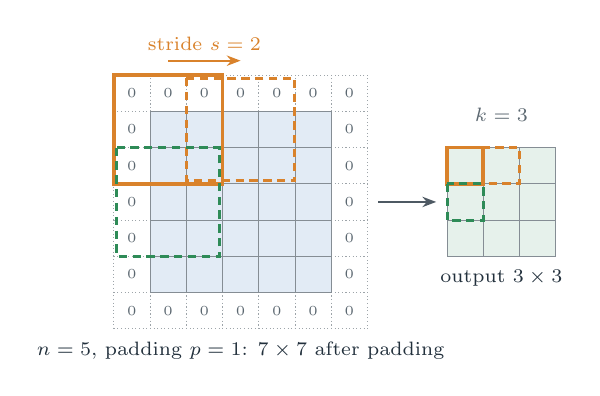
\begin{tikzpicture}[x=4.6mm,y=4.6mm]
  \foreach \r in {0,...,6} \foreach \c in {0,...,6}
    \node[gc=4.6mm,draw=cTok!60,densely dotted,text=cTok,font=\tiny] at (\c,-\r) {0};
  \foreach \r in {1,...,5} \foreach \c in {1,...,5}
    \node[gc=4.6mm,fill=cEmb!14] at (\c,-\r) {};
  \draw[cAtt,line width=1.3pt] (-0.5,0.5) rectangle (2.5,-2.5);
  \draw[cAtt,line width=1.1pt,densely dashed] (1.5,0.42) rectangle (4.5,-2.42);
  \draw[cFfn,line width=1.1pt,densely dashed] (-0.42,-1.5) rectangle (2.42,-4.5);
  \draw[->,cAtt,line width=0.8pt] (1,0.9) -- node[above,note,text=cAtt] {stride $s=2$} (3,0.9);
  \foreach \r in {0,1,2} \foreach \c in {0,1,2} \node[gc=4.6mm,fill=cFfn!12] at (9.2+\c,-2-\r) {};
  \draw[cAtt,line width=1.3pt] (8.7,-1.5) rectangle (9.7,-2.5);
  \draw[cAtt,line width=1.1pt,densely dashed] (9.7,-1.5) rectangle (10.7,-2.5);
  \draw[cFfn,line width=1.1pt,densely dashed] (8.7,-2.5) rectangle (9.7,-3.5);
  \draw[flow] (6.8,-3) -- (8.4,-3);
  \node[note,text=cInk] at (3,-7.1) {$n=5$, padding $p=1$: $7\times7$ after padding};
  \node[note,text=cInk] at (10.2,-5.1) {output $3\times3$};
  \node[note] at (10.2,-0.6) {$k=3$};
\end{tikzpicture}

\vspace{1mm}
\begin{block}{Output size along one axis}
\vspace{-2.5mm}
\[
  n_\text{out}=\Bigl\lfloor\frac{n+2p-k}{s}\Bigr\rfloor+1
\]
\footnotesize $n$ input size, $k$ kernel size, $p$ padding on each side, $s$ stride.
Drawing: $\lfloor(5+2-3)/2\rfloor+1=\num{3}$.
\end{block}
\column{0.53\textwidth}
\small
\begin{itemize}\footnotesize
  \item \key{Padding} $p$: surround the image with $p$ rings of zeros. Without it every layer shrinks the
        map by $k-1$ and border pixels are used less often than central ones.
        ``Same'' padding $p=(k-1)/2$ keeps the size (odd $k$, $s=1$).
  \item \key{Stride} $s$: move the window $s$ pixels at a time. The output is about $s$ times smaller per axis,
        so $s^2$ times cheaper. A strided convolution is a learned way of downsampling.
  \item The floor: last rows and columns are ignored when the window does not fit.
\end{itemize}
\vspace{0.2mm}
{\footnotesize
\renewcommand{\arraystretch}{1.12}
\begin{tabular}{@{}rrrrll@{}}
\toprule
$n$ & $k$ & $p$ & $s$ & $\lfloor(n+2p-k)/s\rfloor+1$ & where\\
\midrule
5 & 3 & 0 & 1 & $\lfloor2\rfloor+1=3$ & slide 3\\
5 & 3 & 1 & 1 & $\lfloor4\rfloor+1=5$ & ``same''\\
28 & 5 & 2 & 1 & $\lfloor27\rfloor+1=28$ & our conv1\\
14 & 5 & 0 & 1 & $\lfloor9\rfloor+1=10$ & our conv2\\
28 & 2 & 0 & 2 & $\lfloor13\rfloor+1=14$ & our pool1\\
8 & 3 & 0 & 2 & $\lfloor2.5\rfloor+1=3$ & last column unused\\
224 & 7 & 3 & 2 & $\lfloor111.5\rfloor+1=112$ & ResNet stem \cite{6}\\
\bottomrule
\end{tabular}}

\vspace{1mm}
{\footnotesize The same formula covers pooling (slide 9). More cases (dilation, transposed convolution): \cite{11}.}
\end{columns}
\end{frame}

% ======================================================================= 6
\begin{frame}{Receptive field: how much of the image one unit can see}
\begin{columns}[T,onlytextwidth]
\column{0.50\textwidth}
\centering
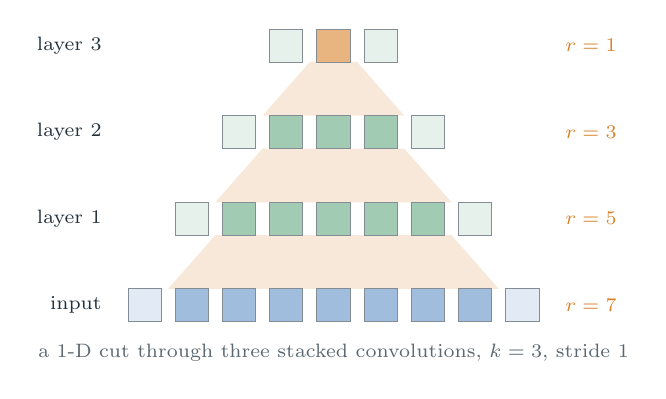
\begin{tikzpicture}[x=6mm,y=11mm]
  \begin{scope}[on background layer]
    \fill[cAtt!18] (0.5,0.19) -- (7.5,0.19) -- (6.5,0.81) -- (1.5,0.81) -- cycle;
    \fill[cAtt!18] (1.5,1.19) -- (6.5,1.19) -- (5.5,1.81) -- (2.5,1.81) -- cycle;
    \fill[cAtt!18] (2.5,2.19) -- (5.5,2.19) -- (4.5,2.81) -- (3.5,2.81) -- cycle;
  \end{scope}
  \foreach \c in {0,...,8} \node[gc=4.2mm,fill=cEmb!14] (i\c) at (\c,0) {};
  \foreach \c in {1,...,7} \node[gc=4.2mm,fill=cFfn!12] at (\c,1) {};
  \foreach \c in {2,...,6} \node[gc=4.2mm,fill=cFfn!12] at (\c,2) {};
  \foreach \c in {3,...,5} \node[gc=4.2mm,fill=cFfn!12] at (\c,3) {};
  \foreach \c in {1,...,7} \node[gc=4.2mm,fill=cEmb!45] at (\c,0) {};
  \foreach \c in {2,...,6} \node[gc=4.2mm,fill=cFfn!45] at (\c,1) {};
  \foreach \c in {3,...,5} \node[gc=4.2mm,fill=cFfn!45] at (\c,2) {};
  \node[gc=4.2mm,fill=cAtt!60] at (4,3) {};
  \foreach \y/\t in {0/input,1/layer 1,2/layer 2,3/layer 3} \node[note,text=cInk,anchor=east] at (-0.7,\y) {\t};
  \foreach \y/\t in {0/{$r=7$},1/{$r=5$},2/{$r=3$},3/{$r=1$}} \node[note,text=cAtt,anchor=west] at (8.7,\y) {\t};
  \node[note] at (4,-0.55) {a 1-D cut through three stacked convolutions, $k=3$, stride 1};
\end{tikzpicture}

\vspace{1.5mm}
\raggedright\footnotesize
The \key{receptive field} of a unit is the set of input pixels that can influence it. One $3\times3$ layer
sees 3 pixels across; each further layer adds $k-1=2$.

\vspace{1mm}
\begin{block}{Recurrence (per axis), from the input upward}
\vspace{-2.5mm}
\[
  r_\ell=r_{\ell-1}+(k_\ell-1)\,j_{\ell-1},\qquad j_\ell=j_{\ell-1}\,s_\ell,\qquad r_0=j_0=1
\]
\footnotesize $j$ (``jump'') is the distance in input pixels between neighbouring units of a layer.
Stride and pooling multiply $j$, so every later layer grows $r$ faster.
\end{block}
\column{0.47\textwidth}
\small
\textbf{Our network} (slide 11)

\vspace{0.5mm}
{\footnotesize
\renewcommand{\arraystretch}{1.12}
\begin{tabular}{@{}lccrcl@{}}
\toprule
layer & $k$ & $s$ & $r$ & $j$ & $r$ computed as\\
\midrule
input & & & 1 & 1 & \\
conv $5\times5$ & 5 & 1 & \num{5} & 1 & $1+4\cdot1$\\
max-pool $2\times2$ & 2 & 2 & \num{6} & 2 & $5+1\cdot1$\\
conv $5\times5$ & 5 & 1 & \num{14} & 2 & $6+4\cdot2$\\
max-pool $2\times2$ & 2 & 2 & \num{16} & 4 & $14+1\cdot2$\\
\bottomrule
\end{tabular}}

\vspace{1.5mm}
{\footnotesize A unit of the last feature map sees a $16\times16$ window of the $28\times28$ image:
enough for a sleeve or a heel, not the whole garment. The linear layers after it combine all 25 positions.}

\vspace{1mm}
\begin{itemize}\footnotesize
  \item \key{Depth builds a hierarchy}: edges, then corners and textures, then parts \cite{12}.
  \item \key{Small kernels, stacked}: two $3\times3$ layers see $5\times5$ with $2\cdot9=18$ weights instead of 25,
        three see $7\times7$ with 27 instead of 49, and they add nonlinearities in between.
        This is the design rule of VGG \cite{5}.
  \item The \emph{effective} receptive field is smaller than $r$: central pixels have many more paths to the
        unit than peripheral ones \cite{16}.
\end{itemize}
\end{columns}
\end{frame}

% ======================================================================= 7
\begin{frame}{Many channels in, many filters out}
\begin{columns}[T,onlytextwidth]
\column{0.50\textwidth}
\centering
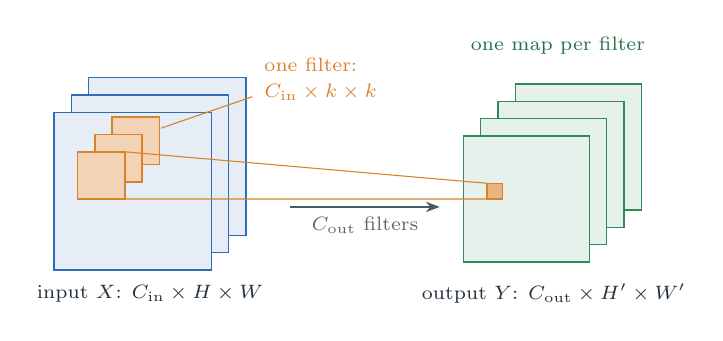
\begin{tikzpicture}[x=1mm,y=1mm]
  % input volume: C_in = 3 slabs
  \foreach \i in {2,1,0} \draw[cEmb,fill=cEmb!12,line width=0.5pt] (\i*2.2,\i*2.2) rectangle ++(20,20);
  \foreach \i in {2,1,0} \draw[cAtt,fill=cAtt!35,line width=0.6pt] (3+\i*2.2,9+\i*2.2) rectangle ++(6,6);
  \node[note,text=cInk] at (12.2,-3) {input $X$: $C_\text{in}\times H\times W$};
  \node[note,text=cAtt,anchor=west] at (25.5,26) {one filter:};
  \node[note,text=cAtt,anchor=west] at (25.5,22.6) {$C_\text{in}\times k\times k$};
  \draw[cAtt,line width=0.4pt] (25.2,22) -- (13.6,18);
  % output volume: C_out = 4 maps
  \foreach \i in {3,2,1,0} \draw[cFfn,fill=cFfn!12,line width=0.5pt] (52+\i*2.2,1+\i*2.2) rectangle ++(16,16);
  \draw[cAtt,fill=cAtt!60,line width=0.5pt] (55,9) rectangle ++(2,2);
  \draw[cAtt,line width=0.4pt] (9,15) -- (55,11) (9,9) -- (55,9);
  \node[note,text=cInk] at (63.5,-3) {output $Y$: $C_\text{out}\times H'\times W'$};
  \node[note,text=cFfn!80!black] at (64,28.5) {one map per filter};
  \draw[flow] (30,8) -- node[below,note] {$C_\text{out}$ filters} (49,8);
\end{tikzpicture}

\vspace{0.5mm}
\begin{block}{The convolution layer in full}
\vspace{-2.5mm}
\[
  Y_{o,i,j}=b_o+\sum_{c=0}^{C_\text{in}-1}\;\sum_{u=0}^{k-1}\sum_{v=0}^{k-1}W_{o,c,u,v}\;X_{c,\;si+u,\;sj+v}
\]
\footnotesize Weight tensor $W\in\R^{C_\text{out}\times C_\text{in}\times k\times k}$, bias $b\in\R^{C_\text{out}}$;
$X$ is the padded input, $s$ the stride. In PyTorch: \texttt{nn.Conv2d(C\_in, C\_out, k)}, whose
\texttt{weight.shape} is $(C_\text{out},C_\text{in},k,k)$.
\end{block}
\column{0.47\textwidth}
\small
\begin{itemize}\footnotesize
  \item A filter is a small \textbf{volume}: it spans \emph{all} input channels but only $k\times k$ pixels.
        One output value is the dot product of that volume with the patch under it.
  \item Each filter yields one \key{feature map}. $C_\text{out}$ filters give $C_\text{out}$ maps, which are
        the input channels of the next layer.
  \item Typical pattern: spatial size goes down, channel count goes up.
\end{itemize}
\vspace{-0.5mm}
\begin{block}{Counting parameters: $C_\text{out}\,(C_\text{in}\,k^2+1)$}
\footnotesize
\renewcommand{\arraystretch}{1.1}
\begin{tabular}{@{}lll@{}}
our conv1 & $(8,1,5,5)$ & $8\,(1\cdot25+1)=\num{208}$\\
our conv2 & $(16,8,5,5)$ & $16\,(8\cdot25+1)=\num{3{,}216}$\\
RGB, 64 filters & $(64,3,3,3)$ & $64\,(3\cdot9+1)=\num{1{,}792}$\\
\end{tabular}

\vspace{0.8mm}
The count does not depend on $H$ or $W$. A dense layer from 784 pixels to the $8\cdot28\cdot28=6{,}272$
outputs of conv1 would need 4{,}923{,}520 parameters instead of 208.
\end{block}
{\footnotesize \key{$1\times1$ convolution}: $k=1$ mixes channels at each pixel separately; it is a dense
layer applied at every position, used to change the channel count cheaply \cite{10}.}
\end{columns}
\end{frame}

% ======================================================================= 8
\begin{frame}{Weight sharing and translation equivariance}
\begin{columns}[T,onlytextwidth]
\column{0.50\textwidth}
\centering
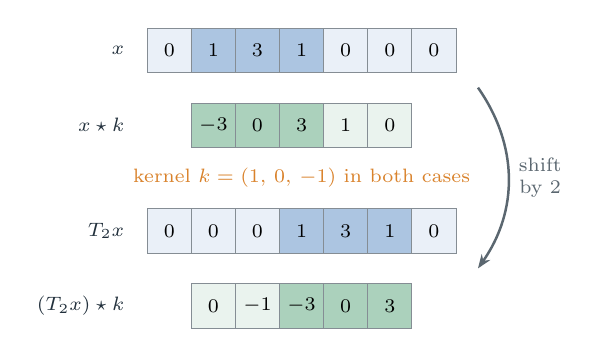
\begin{tikzpicture}[x=5.6mm,y=5.6mm]
  \node[note,text=cInk,anchor=east] at (-0.8,0) {$x$};
  \cellrow{0}{0}{gc=5.6mm,fill=cEmb!10}{0,1,3,1,0,0,0}
  \foreach \c/\v in {1/1,2/3,3/1} \node[gc=5.6mm,fill=cEmb!40] at (\c,0) {\v};
  \node[note,text=cInk,anchor=east] at (-0.8,-1.7) {$x\xcorr k$};
  \cellrow{1}{1.7}{gc=5.6mm,fill=cFfn!10}{$-3$,0,3,1,0}
  \foreach \c/\v in {1/$-3$,2/0,3/3} \node[gc=5.6mm,fill=cFfn!40] at (\c,-1.7) {\v};
  \node[note,text=cInk,anchor=east] at (-0.8,-4.1) {$T_2x$};
  \cellrow{0}{4.1}{gc=5.6mm,fill=cEmb!10}{0,0,0,1,3,1,0}
  \foreach \c/\v in {3/1,4/3,5/1} \node[gc=5.6mm,fill=cEmb!40] at (\c,-4.1) {\v};
  \node[note,text=cInk,anchor=east] at (-0.8,-5.8) {$(T_2x)\xcorr k$};
  \cellrow{1}{5.8}{gc=5.6mm,fill=cFfn!10}{0,$-1$,$-3$,0,3}
  \foreach \c/\v in {3/$-3$,4/0,5/3} \node[gc=5.6mm,fill=cFfn!40] at (\c,-5.8) {\v};
  \node[note,text=cAtt] at (3,-2.9) {kernel $k=(1,\,0,\,-1)$ in both cases};
  \draw[->,cTok,line width=0.9pt] (7.0,-0.85) to[bend left=35] node[right,note] {shift\\by 2} (7.0,-4.95);
\end{tikzpicture}

\vspace{1mm}
\raggedright\footnotesize
Shifting the input by 2 shifts the output by 2 (dark cells). What is pushed past the border is lost
(the 1 near the end of the first output); a new value enters on the other side.
\begin{block}{Translation equivariance}
\vspace{-2.5mm}
\[
  (T_a x)\xcorr k\;=\;T_a\,(x\xcorr k)\qquad\text{$T_a$: shift by $a$ pixels}
\]
\footnotesize Exact away from the border. It follows from the definition: the weights $K_{u,v}$ do not depend
on the position $(i,j)$.
\end{block}
\column{0.47\textwidth}
\small
\begin{itemize}\footnotesize
  \item \key{Weight sharing}: every position uses the same kernel. A feature learned in one corner is
        detected everywhere, with no extra parameters or training examples.
  \item \key{Equivariant} is not \key{invariant}. Equivariant: the feature map moves with the object.
        Invariant: the answer does not change. Classification wants invariance; pooling and the head
        (slides 9, 10) must turn one into the other.
\end{itemize}
\vspace{-0.5mm}
\begin{block}{Measured on a real image (experiment C)}
\footnotesize
Test image 0 shifted 2 pixels down, 3 right; four random $5\times5$ kernels, padding 2.\\[0.6mm]
\renewcommand{\arraystretch}{1.1}
\begin{tabular}{@{}p{58mm}r@{}}
$\max\bigl|(T x)\xcorr K-T(x\xcorr K)\bigr|$, interior & \textbf{\equivInterior}\\
same, including the border rows and columns & \equivBorder\\
random dense layer, $\lVert W\,Tx-Wx\rVert/\lVert Wx\rVert$ & \denseChange\%\\
\end{tabular}

\vspace{0.6mm}
The interior agrees to the last bit. A dense layer has no output positions that could move:
its response to the shifted image is just a different vector.
\end{block}
{\footnotesize Caveat: with stride or pooling this holds only for shifts by multiples of the total stride,
and a trained CNN is \emph{not} shift-invariant \cite{15}. Slide 14 measures it.}
\end{columns}
\end{frame}

% ======================================================================= 9
\begin{frame}{Nonlinearity and pooling}
\begin{columns}[T,onlytextwidth]
\column{0.52\textwidth}
\centering
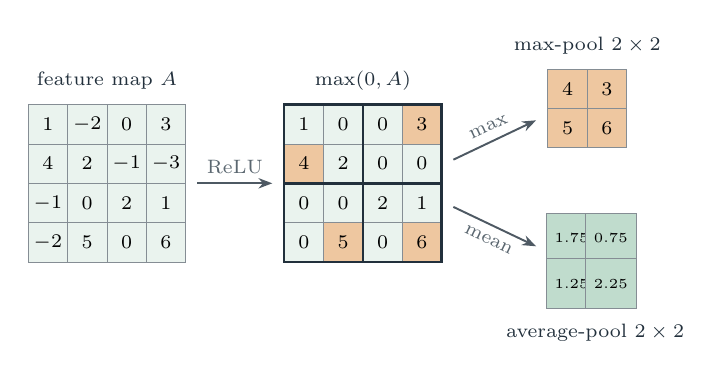
\begin{tikzpicture}[x=5mm,y=5mm]
  \cellrow{0}{0}{gc=5mm,fill=cFfn!10}{1,$-2$,0,3}
  \cellrow{0}{1}{gc=5mm,fill=cFfn!10}{4,2,$-1$,$-3$}
  \cellrow{0}{2}{gc=5mm,fill=cFfn!10}{$-1$,0,2,1}
  \cellrow{0}{3}{gc=5mm,fill=cFfn!10}{$-2$,5,0,6}
  \node[note,text=cInk] at (1.5,1.1) {feature map $A$};
  \draw[flow] (3.8,-1.5) -- node[above,note] {ReLU} (5.7,-1.5);
  \cellrow{6.5}{0}{gc=5mm,fill=cFfn!10}{1,0,0,3}
  \cellrow{6.5}{1}{gc=5mm,fill=cFfn!10}{4,2,0,0}
  \cellrow{6.5}{2}{gc=5mm,fill=cFfn!10}{0,0,2,1}
  \cellrow{6.5}{3}{gc=5mm,fill=cFfn!10}{0,5,0,6}
  \foreach \c/\r/\v in {6.5/1/4,9.5/0/3,7.5/3/5,9.5/3/6} \node[gc=5mm,fill=cAtt!45] at (\c,-\r) {\v};
  \draw[cInk,line width=0.9pt] (6,0.5) rectangle (10,-3.5) (8,0.5) -- (8,-3.5) (6,-1.5) -- (10,-1.5);
  \node[note,text=cInk] at (8,1.1) {$\max(0,A)$};
  \draw[flow] (10.3,-0.9) -- node[above,note,sloped] {max} (12.4,0.1);
  \draw[flow] (10.3,-2.1) -- node[below,note,sloped] {mean} (12.4,-3.1);
  \cellrow{13.2}{-0.9}{gc=5mm,fill=cAtt!45}{4,3}
  \cellrow{13.2}{0.1}{gc=5mm,fill=cAtt!45}{5,6}
  \cellrow{13.3}{2.9}{gc=6.4mm,fill=cFfn!30,font=\tiny}{1.75,0.75}
  \cellrow{13.3}{4.05}{gc=6.4mm,fill=cFfn!30,font=\tiny}{1.25,2.25}
  \node[note,text=cInk] at (13.7,2.0) {max-pool $2\times2$};
  \node[note,text=cInk] at (13.9,-5.3) {average-pool $2\times2$};
\end{tikzpicture}

\vspace{0.5mm}
\raggedright\footnotesize
\key{ReLU}, $\max(0,a)$, applied to every value. Without a nonlinearity two convolutions in a row
collapse into one larger convolution (linear after linear is linear). A zero means
``this feature is absent here''.

\vspace{1mm}
\key{Pooling} summarises each $2\times2$ block (kernel 2, stride 2) of each channel separately,
by its maximum or its mean:
\[
  \pool(A)_{i,j}=\max_{0\le u,v<2}A_{2i+u,\,2j+v}\,.
\]
\vspace{-3.5mm}

Output size (slide 5): $\lfloor(4-2)/2\rfloor+1=2$. No parameters.
\column{0.45\textwidth}
\small
\begin{itemize}\footnotesize
  \item \textbf{Why pool?} It removes 75\% of the values, so later layers are four times
        cheaper, and it doubles the jump $j$ of slide 6: the receptive field grows faster.
  \item \textbf{A little invariance}: if the 4 in the top-left block moves to another cell
        of its block, the max-pooled output is unchanged. A first step from equivariance to invariance.
  \item \textbf{Max or average?} Max: ``is the feature anywhere in the block?'' Average:
        ``how much of it?'' Max is the usual choice inside a network.
  \item Many modern networks downsample with stride-2 convolutions instead \cite{6}.
\end{itemize}
\vspace{-0.5mm}
\begin{block}{Global average pooling (GAP) \cite{10}}
\footnotesize
Average each channel over \emph{all} positions: $C\times H\times W\to C$ numbers. For the map above:
$24/16=\num{1.5}$. It replaces the large flatten-plus-dense head: with a GAP head our network has
\paramsGap{} parameters instead of \paramsCnn{} (\texttt{CNN(head="gap")}), and accepts any input size.
\end{block}
\end{columns}
\end{frame}

% ====================================================================== 10
\begin{frame}{The classifier head: flatten, linear, softmax, cross-entropy}
\centering
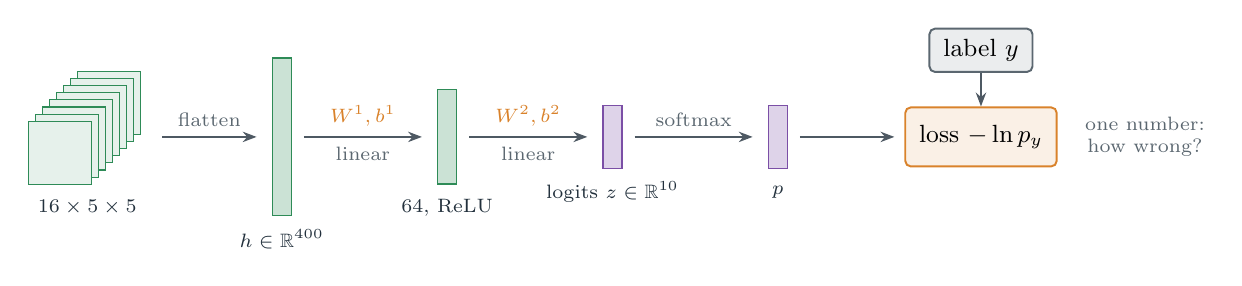
\begin{tikzpicture}[x=1mm,y=1mm]
  \foreach \i in {7,...,0} \draw[cFfn,fill=cFfn!12,line width=0.4pt] (\i*0.9,\i*0.9) rectangle ++(8,8);
  \node[note,text=cInk] at (7.5,-3) {$16\times5\times5$};
  \draw[flow] (17,6) -- node[above,note] {flatten} (29,6);
  \draw[cFfn,fill=cFfn!25,line width=0.5pt] (31,-4) rectangle ++(2.4,20); \node[note,text=cInk] at (32.2,-7) {$h\in\R^{400}$};
  \draw[flow] (35,6) -- node[above,note,text=cAtt] {$W^1,b^1$} node[below,note] {linear} (50,6);
  \draw[cFfn,fill=cFfn!25,line width=0.5pt] (52,0) rectangle ++(2.4,12); \node[note,text=cInk] at (53.2,-3) {64, ReLU};
  \draw[flow] (56,6) -- node[above,note,text=cAtt] {$W^2,b^2$} node[below,note] {linear} (71,6);
  \draw[cOut,fill=cOut!25,line width=0.5pt] (73,2) rectangle ++(2.4,8); \node[note,text=cInk] at (74.2,-1) {logits $z\in\R^{10}$};
  \draw[flow] (77,6) -- node[above,note] {softmax} (92,6);
  \draw[cOut,fill=cOut!25,line width=0.5pt] (94,2) rectangle ++(2.4,8); \node[note,text=cInk] at (95.2,-1) {$p$};
  \draw[flow] (98,6) -- (110,6);
  \node[stage=cAtt] (L) at (121,6) {loss $-\ln p_y$};
  \node[stage=cTok,minimum height=5.5mm] (y) at (121,17) {label $y$};
  \draw[flow] (y) -- (L);
  \node[note,anchor=west] at (133,6) {one number:\\how wrong?};
\end{tikzpicture}

\vspace{1.5mm}
\begin{columns}[T,onlytextwidth]
\column{0.37\textwidth}
\footnotesize
\begin{itemize}
  \item \key{Flatten}: write the $16\cdot5\cdot5$ values as one vector of 400; an ordinary MLP follows.
  \item \key{Logits} $z=W^2\ReLU(W^1h+b^1)+b^2$: one raw score per class.
  \item \key{Softmax} turns scores into probabilities:
  \[ p_k=\frac{e^{z_k}}{\sum_{j}e^{z_j}},\qquad p_k>0,\ \ \textstyle\sum_k p_k=1. \]
  \vspace{-3mm}
  \item \key{Cross-entropy} loss for true class $y$:
  \[ \mathcal L=-\ln p_y,\qquad \frac{\partial\mathcal L}{\partial z}=p-\operatorname{onehot}(y). \]
\end{itemize}
\column{0.30\textwidth}
\centering
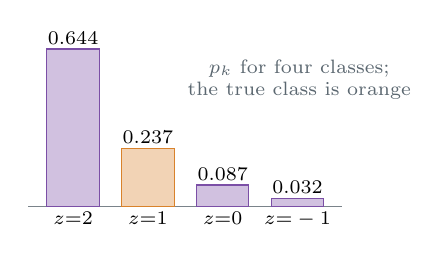
\begin{tikzpicture}[x=9.5mm,y=31mm,font=\scriptsize]
  \draw[cInk!60] (-0.1,0) -- (4.1,0);
  \foreach \i/\p/\z/\c in {0/0.644/2/cOut,1/0.237/1/cAtt,2/0.087/0/cOut,3/0.032/{-1}/cOut} {
    \draw[\c,fill=\c!35] (\i+0.15,0) rectangle (\i+0.85,\p);
    \node[above,inner sep=1.5pt] at (\i+0.5,\p) {\p};
    \node[below,inner sep=2pt] at (\i+0.5,0) {$z{=}\z$};}
  \node[note,anchor=west] at (1.9,0.52) {$p_k$ for four classes;\\the true class is orange};
\end{tikzpicture}

\vspace{1mm}
{\footnotesize Untrained, all $p_k\approx\tfrac1{10}$:\\the loss starts near $\ln10=\num{2.30}$.}
\column{0.29\textwidth}
\begin{block}{By hand (4 classes)}
\footnotesize
$z=(2,\,1,\,0,\,-1)$\\[0.4mm]
$e^{z}=(7.389,\,2.718,\,1,\,0.368)$, sum $11.475$\\[0.4mm]
$p=(0.644,\,0.237,\,0.087,\,0.032)$\\[0.4mm]
True class is the 2nd: $\mathcal L=-\ln0.237=\num{1.440}$\\[0.4mm]
$\partial\mathcal L/\partial z=(0.644,{-0.763},0.087,0.032)$:
raise the true score, lower the rest.
\end{block}
\end{columns}
\end{frame}

% ====================================================================== 11
\begin{frame}{The complete network: a LeNet-style CNN, shape by shape}
\centering
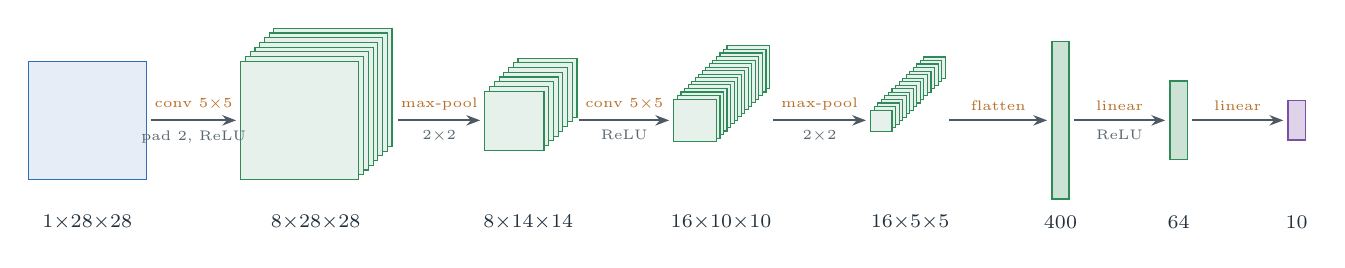
\begin{tikzpicture}[x=1mm,y=1mm]
  % stacks: x position / number of slabs / side / slab offset / colour
  \draw[cEmb,fill=cEmb!12,line width=0.4pt] (0,0) rectangle ++(15,15);
  \foreach \i in {7,...,0} \draw[cFfn,fill=cFfn!12,line width=0.4pt] (27+\i*0.6,\i*0.6) rectangle ++(15,15);
  \foreach \i in {7,...,0} \draw[cFfn,fill=cFfn!12,line width=0.4pt] (58+\i*0.6,3.7+\i*0.6) rectangle ++(7.5,7.5);
  \foreach \i in {15,...,0} \draw[cFfn,fill=cFfn!12,line width=0.4pt] (82+\i*0.45,4.8+\i*0.45) rectangle ++(5.4,5.4);
  \foreach \i in {15,...,0} \draw[cFfn,fill=cFfn!12,line width=0.4pt] (107+\i*0.45,6.1+\i*0.45) rectangle ++(2.7,2.7);
  \draw[cFfn,fill=cFfn!25,line width=0.5pt] (130,-2.5) rectangle ++(2.2,20);
  \draw[cFfn,fill=cFfn!25,line width=0.5pt] (145,2.5) rectangle ++(2.2,10);
  \draw[cOut,fill=cOut!25,line width=0.5pt] (160,5) rectangle ++(2.2,5);
  \foreach \a/\b/\t/\u in {15.6/26.4/{conv $5{\times}5$}/{pad 2, ReLU},47/57.4/{max-pool}/{$2{\times}2$},
      70/81.4/{conv $5{\times}5$}/{ReLU},94.6/106.4/{max-pool}/{$2{\times}2$},117/129.4/flatten/{},
      132.8/144.4/linear/{ReLU},147.8/159.4/linear/{}}
    \draw[flow] (\a,7.5) -- node[above,note,text=cAtt!85!black,font=\tiny] {\t} node[below,note,font=\tiny] {\u} (\b,7.5);
  \foreach \x/\t in {7.5/{$1{\times}28{\times}28$},36.5/{$8{\times}28{\times}28$},63.5/{$8{\times}14{\times}14$},
      88/{$16{\times}10{\times}10$},112/{$16{\times}5{\times}5$},131.1/{400},146.1/{64},161.1/{10}}
    \node[note,text=cInk] at (\x,-5.5) {\t};
\end{tikzpicture}

\vspace{1.5mm}
\begin{columns}[T,onlytextwidth]
\column{0.50\textwidth}
\centering
{\footnotesize
\renewcommand{\arraystretch}{1.07}\setlength{\tabcolsep}{4.5pt}
\begin{tabular}{@{}llrr@{}}
\toprule
layer & output $(C,H,W)$ & values & parameters\\
\midrule
\archRows
\midrule
total & & & \textbf{\paramsCnn}\\
\bottomrule
\end{tabular}}

\vspace{0.5mm}
{\scriptsize\color{cTok}Generated from \texttt{shape\_table(CNN())} in \texttt{cnn.py}; the column sum is checked against the model.}
\column{0.47\textwidth}
\footnotesize
\begin{itemize}
  \item The pattern is LeNet's \cite{2,3}: [convolution, nonlinearity, pooling] twice, then dense layers.
        LeNet-5 used tanh-like units and trainable subsampling instead of ReLU and max-pooling.
  \item \textbf{Parameters}: the two convolutions hold \paramsConv{} (\paramsConvShare\%); the first
        dense layer alone holds 25{,}664.
  \item \textbf{Arithmetic}: conv2 does $1{,}600\cdot200=320{,}000$ multiplications per image,
        conv1 $6{,}272\cdot25=156{,}800$, both dense layers together $26{,}240$. Convolutions are cheap in
        parameters, not in computation.
  \item \textbf{Baselines} (slide 17): an MLP $784\to128\to64\to10$ with \paramsMlp{} parameters
        (\paramRatio{} times more) and softmax regression $784\to10$ with \paramsLin.
\end{itemize}
\end{columns}
\end{frame}

% ====================================================================== 12
\begin{frame}{Backpropagation through a convolution}
\begin{columns}[T,onlytextwidth]
\column{0.47\textwidth}
\small
Forward: $Y=X\xcorr K+b$. The layer above hands us $\delta=\partial\mathcal L/\partial Y$, one number per
output position.
\begin{block}{Backward pass of one convolution (stride 1)}
\vspace{-3mm}
\begin{align*}
 \frac{\partial\mathcal L}{\partial K_{u,v}} &= \sum_{i,j}\delta_{i,j}\,X_{i+u,\,j+v}
     &&\Longleftrightarrow\quad \frac{\partial\mathcal L}{\partial K}=X\xcorr\delta\\
 \frac{\partial\mathcal L}{\partial X_{m,n}} &= \sum_{u,v}\delta_{m-u,\,n-v}\,K_{u,v}
     &&\Longleftrightarrow\quad \frac{\partial\mathcal L}{\partial X}=\delta * K\\
 \frac{\partial\mathcal L}{\partial b} &= \sum_{i,j}\delta_{i,j}
\end{align*}
\end{block}
\begin{itemize}\footnotesize
  \item \textbf{Kernel gradient}: the input correlated with the error map. The kernel is shared, so
        its gradient is a \emph{sum over all positions}.
  \item \textbf{Input gradient}: a true (flipped, ``full'') convolution: pad $\delta$ by $k-1$ and
        correlate with $K$ rotated by $180^\circ$. This flows on to the layer below.
  \item \textbf{ReLU}: pass $\delta$ where the input was positive. \textbf{Max-pool}: send $\delta$ to
        the cell that held the maximum.
\end{itemize}
\column{0.50\textwidth}
\centering
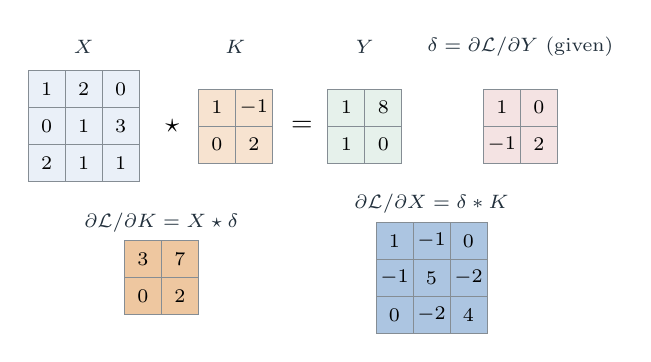
\begin{tikzpicture}[x=4.7mm,y=4.7mm]
  \cellrow{0}{0}{gc=4.7mm,fill=cEmb!10}{1,2,0} \cellrow{0}{1}{gc=4.7mm,fill=cEmb!10}{0,1,3}
  \cellrow{0}{2}{gc=4.7mm,fill=cEmb!10}{2,1,1}
  \node at (3.4,-1) {$\xcorr$};
  \cellrow{4.6}{0.5}{gc=4.7mm,fill=cAtt!22}{1,$-1$} \cellrow{4.6}{1.5}{gc=4.7mm,fill=cAtt!22}{0,2}
  \node at (6.9,-1) {$=$};
  \cellrow{8.1}{0.5}{gc=4.7mm,fill=cFfn!12}{1,8} \cellrow{8.1}{1.5}{gc=4.7mm,fill=cFfn!12}{1,0}
  \cellrow{12.3}{0.5}{gc=4.7mm,fill=cBad!14}{1,0} \cellrow{12.3}{1.5}{gc=4.7mm,fill=cBad!14}{$-1$,2}
  \node[note,text=cInk] at (1,1.15) {$X$}; \node[note,text=cInk] at (5.1,1.15) {$K$};
  \node[note,text=cInk] at (8.6,1.15) {$Y$}; \node[note,text=cInk] at (12.8,1.15) {$\delta=\partial\mathcal L/\partial Y$ (given)};
  \cellrow{2.6}{4.6}{gc=4.7mm,fill=cAtt!45}{3,7} \cellrow{2.6}{5.6}{gc=4.7mm,fill=cAtt!45}{0,2}
  \node[note,text=cInk] at (3.1,-3.6) {$\partial\mathcal L/\partial K=X\xcorr\delta$};
  \cellrow{9.4}{4.1}{gc=4.7mm,fill=cEmb!40}{1,$-1$,0} \cellrow{9.4}{5.1}{gc=4.7mm,fill=cEmb!40}{$-1$,5,$-2$}
  \cellrow{9.4}{6.1}{gc=4.7mm,fill=cEmb!40}{0,$-2$,4}
  \node[note,text=cInk] at (10.4,-3.1) {$\partial\mathcal L/\partial X=\delta*K$};
\end{tikzpicture}

\vspace{0.5mm}
\raggedright\footnotesize
\textbf{Check two entries.}
$\partial\mathcal L/\partial K_{0,0}=1\cdot1+0\cdot2+(-1)\cdot0+2\cdot1=\num{3}$ ($\delta$ times the top-left
$2\times2$ patch of $X$). The centre pixel $X_{1,1}$ feeds all four outputs:
$1\cdot2+0\cdot0+(-1)(-1)+2\cdot1=\num{5}$.
\begin{block}{Measured: \texttt{conv2d\_backward} (experiment E)}
\footnotesize
\renewcommand{\arraystretch}{1.1}
\begin{tabular}{@{}p{64mm}r@{}}
vs.\ centred finite differences: worst relative error over $x$, $w$, $b$ and three stride/padding settings & $\gradFD$\\
vs.\ PyTorch autograd: worst absolute difference & $\gradTorch$\\
\end{tabular}

\vspace{0.4mm}
The code handles any stride and padding ($X_{si+u,\,sj+v}$ in the sums).
\end{block}
\end{columns}
\end{frame}

% ====================================================================== 13
\begin{frame}{Training: mini-batches, optimizer, learning rate}
\begin{columns}[T,onlytextwidth]
\column{0.49\textwidth}
\centering
\begin{tikzpicture}
\begin{axis}[width=8.3cm,height=4.2cm,xmin=0.5,xmax=12.5,ymin=0,ymax=0.65,
  xlabel={epoch},ylabel={loss (cross-entropy)},label style={font=\scriptsize},tick label style={font=\tiny},
  axis lines=left,ymajorgrids,grid style={cInk!10},xtick={1,...,12},
  legend style={font=\scriptsize,draw=none,fill=none,at={(0.98,0.98)},anchor=north east},legend cell align=left,
  every axis plot/.append style={line width=1.1pt,mark size=1.3pt}]
  \addplot[cEmb,mark=*] table[x=epoch,y=train]{generated/curves.dat}; \addlegendentry{training loss}
  \addplot[cAtt,mark=square*] table[x=epoch,y=val]{generated/curves.dat}; \addlegendentry{validation loss}
  \draw[cInk,dashed] (axis cs:\bestEpoch,0) -- (axis cs:\bestEpoch,0.3);
  \node[font=\tiny,anchor=north east,text=cInk,inner sep=1.5pt] at (axis cs:\bestEpoch,0.12) {best checkpoint};
\end{axis}
\end{tikzpicture}

\vspace{-0.5mm}
{\scriptsize\color{cTok}Measured: CNN of slide 11, seed 0, Adam, $\eta=0.002$, batch 64; training loss on 2{,}000
training images. One run.}

\vspace{0.8mm}
\raggedright\footnotesize
\begin{itemize}
  \item \key{Mini-batch SGD}: estimate the gradient on $B$ images, step, repeat:
        $\theta\leftarrow\theta-\eta\,\nabla_\theta\frac1B\sum_{n=1}^{B}\mathcal L_n$.
        With $B=64$, one \key{epoch} over \nTrain{} images is 157 steps.
  \item \key{Validation} after every epoch. Keep the weights of the best epoch (here \bestEpoch, loss \bestVal);
        stop after 3 epochs without improvement.
  \item The gap between the curves is \textbf{overfitting}: after epoch \epochsCnn{} the training loss is
        \lastTrain, the validation loss \lastVal{} (slide 14).
\end{itemize}
\column{0.48\textwidth}
\centering
\begin{tikzpicture}
\begin{semilogxaxis}[width=8.3cm,height=4.2cm,xmin=0.0002,xmax=1.5,ymin=0.4,ymax=2.75,
  xlabel={learning rate $\eta$},ylabel={validation loss after 2 epochs},label style={font=\scriptsize},
  tick label style={font=\tiny},axis lines=left,ymajorgrids,grid style={cInk!10},
  xtick={0.0003,0.001,0.003,0.01,0.03,0.1,0.3,1},xticklabels={.0003,.001,.003,.01,.03,.1,.3,1},
  legend style={font=\scriptsize,draw=none,fill=none,at={(0.04,0.62)},anchor=west},legend cell align=left,
  every axis plot/.append style={line width=1.1pt,mark size=1.5pt}]
  \addplot[cTok,mark=*] table[x=lr,y=sgd]{generated/lr.dat}; \addlegendentry{plain SGD}
  \addplot[cFfn,mark=triangle*] table[x=lr,y=adam]{generated/lr.dat}; \addlegendentry{Adam}
  \draw[cBad,dashed] (axis cs:0.0002,2.303) -- (axis cs:1.5,2.303);
  \node[font=\tiny,text=cBad,anchor=south west] at (axis cs:0.00022,2.33) {$\ln10$: no better than guessing};
\end{semilogxaxis}
\end{tikzpicture}

\vspace{-0.5mm}
{\scriptsize\color{cTok}Measured: same CNN, 3{,}000 training images, 2 epochs, one run per point (experiment F). Values above 2.5 are drawn at 2.5.}

\vspace{0.8mm}
\raggedright\footnotesize
\begin{itemize}
  \item The \key{learning rate} $\eta$ matters most. Too small: little happens in the time
        available. Too large: an early step throws the weights so far that every image gets the same
        answer; the loss stays at $\ln10$.
  \item \key{Adam} \cite{9} divides each weight's step by the root of a running average of its squared
        gradient. It reaches a loss below 1 here for $\eta$ from \lrAdamRange, plain SGD only from \lrSgdRange.
  \item Everywhere else: Adam, $\eta=0.002$, no schedule.
\end{itemize}
\end{columns}
\end{frame}

% ====================================================================== 14
\begin{frame}{Regularisation, normalisation, augmentation: what actually helped}
\begin{columns}[T,onlytextwidth]
\column{0.47\textwidth}
\footnotesize
\key{Batch normalisation} \cite{7}, after a convolution. Per channel $c$, with mean $\mu_c$ and
std $\sigma_c$ over the batch and all positions:
\[
  \hat x=\frac{x-\mu_c}{\sigma_c},\qquad y=\gamma_c\,\hat x+\beta_c\qquad(\gamma_c,\beta_c\text{ learned})
\]
\vspace{-4mm}

Example: $(1,3,5,7)\to\hat x=(-1.34,-0.45,0.45,1.34)$. Test time: running averages.

\vspace{0.8mm}
\key{Dropout} \cite{8}, before the last layer. In training, zero each hidden activation with
probability $p=0.3$, divide the rest by $1-p$. Off at test time.

\vspace{0.8mm}
\key{Data augmentation.} Each time an image is used, shift it by a random $(d_y,d_x)$,
$|d_y|,|d_x|\le2$ pixels: 25 variants per image, same label.

\vspace{0.8mm}
\textbf{Honest reading of the measurements}
\begin{itemize}
  \item Batch norm and dropout did not improve test accuracy here (12 epochs, \nTrain{} images): rows 1--3
        differ by less than the seed noise, $\pm\accCnnStd$.
  \item Augmentation \emph{lowered} centred-test accuracy, shrank the train--validation gap and
        bought robustness to shifts.
  \item Without it, a 2-pixel shift takes the CNN from \shiftZeroCnn\% to \shiftTwoCnn\%, the MLP from
        \shiftZeroMlp\% to \shiftTwoMlp\%: neither is invariant \cite{15}.
\end{itemize}
\column{0.50\textwidth}
\centering
{\footnotesize\renewcommand{\arraystretch}{1.06}\setlength{\tabcolsep}{4.5pt}
\begin{tabular}{@{}lcccc@{}}
\toprule
CNN variant & val.\ & test & test, 2-px & val $-$ train\\[-1.5pt]
(seed 0, accuracy in \%) & acc.\ & acc.\ & shift & loss\\
\midrule
plain (slide 11) & \ablPlainVal & \ablPlainTest & \ablPlainShiftTwo & \ablPlainGap\\
+ batch norm & \ablBnVal & \ablBnTest & \ablBnShiftTwo & \ablBnGap\\
+ dropout 0.3 & \ablDropVal & \ablDropTest & \ablDropShiftTwo & \ablDropGap\\
+ shifts $\pm2$ px & \ablAugVal & \ablAugTest & \textbf{\ablAugShiftTwo} & \ablAugGap\\
all three & \ablAllVal & \ablAllTest & \textbf{\ablAllShiftTwo} & \ablAllGap\\
\bottomrule
\end{tabular}}

\vspace{1.5mm}
\begin{tikzpicture}
\begin{axis}[width=8.6cm,height=4.3cm,xmin=-0.15,xmax=4.15,ymin=18,ymax=92,ytick={20,40,60,80},
  xlabel={test images shifted by $s$ pixels},ylabel={accuracy (\%)},label style={font=\scriptsize},
  tick label style={font=\tiny},axis lines=left,ymajorgrids,grid style={cInk!10},xtick={0,1,2,3,4},
  legend style={font=\tiny,draw=none,fill=none,at={(0.02,0.0)},anchor=south west,row sep=-1.5pt},legend cell align=left,
  legend columns=1,every axis plot/.append style={line width=1.0pt,mark size=1.3pt},ylabel shift=-3pt]
  \addplot[cFfn,mark=*] table[x=s,y=cnnaug]{generated/shift.dat}; \addlegendentry{CNN + shift aug.}
  \addplot[cOut,mark=triangle*] table[x=s,y=mlpaug]{generated/shift.dat}; \addlegendentry{MLP + shift aug.}
  \addplot[cFfn,dashed,mark=o,mark options={solid}] table[x=s,y=cnn]{generated/shift.dat}; \addlegendentry{CNN}
  \addplot[cOut,dashed,mark=triangle,mark options={solid}] table[x=s,y=mlp]{generated/shift.dat}; \addlegendentry{MLP}
  \addplot[cTok,densely dotted,mark=x,mark options={solid}] table[x=s,y=linear]{generated/shift.dat}; \addlegendentry{softmax regr.}
\end{axis}
\end{tikzpicture}

\vspace{-1mm}
{\scriptsize\color{cTok}Measured (experiments G, H). First \shiftN{} test images, mean of the 4 shift
directions. Dashed and dotted: mean of 3 seeds; solid: seed 0.}
\end{columns}
\end{frame}

% ====================================================================== 15
\begin{frame}[fragile]{Code: convolution from scratch in NumPy (forward and backward)}
\vspace{-1mm}
{\footnotesize \texttt{conv\_numpy.py}: the forward pass of slide 7 and the backward pass of slide 12
(lines verbatim; three lines of shape bookkeeping omitted)}
\lstinputlisting[style=py,basicstyle=\ttfamily\fontsize{5.7}{6.8}\selectfont,linerange={21-22,26-34}]{../conv_numpy.py}
\lstinputlisting[style=py,basicstyle=\ttfamily\fontsize{5.7}{6.8}\selectfont,linerange={37-37,40-49}]{../conv_numpy.py}
\vspace{0.5mm}
{\footnotesize
\textbf{Checked} (\texttt{python conv\_numpy.py}, \texttt{test\_cnn.py}): forward equals \texttt{torch.nn.functional.conv2d}
to $\fwdTorch$; backward equals autograd to $\gradTorch$ and finite differences to $\gradFD$. The trained
network run through these functions plus \texttt{pool2d} (\texttt{cnn\_forward}) reproduces the PyTorch logits.
The loops are for reading; \texttt{conv2d\_windows} does the same without them.}
\end{frame}

% ====================================================================== 16
\begin{frame}[fragile]{Code: the model and the training loop in PyTorch}
\vspace{-1mm}
{\footnotesize \texttt{cnn.py}: the network of slide 11 (\texttt{norm} is batch norm or nothing; \texttt{c1, c2 = 8, 16})}
\lstinputlisting[style=py,basicstyle=\ttfamily\fontsize{5.7}{6.8}\selectfont,linerange={24-29,31-36}]{../cnn.py}
\vspace{0.3mm}
{\footnotesize \texttt{train.py}, inside \texttt{fit()} (augmentation and logging omitted). Afterwards the best weights are
restored and \texttt{evaluate()} reports test accuracy, the confusion matrix and a one-class baseline.}
\lstinputlisting[style=py,basicstyle=\ttfamily\fontsize{5.7}{6.8}\selectfont,linerange={84-86,89-93,95-96,105-107}]{../train.py}
\end{frame}

% ====================================================================== 17
\begin{frame}{Results: CNN vs.\ MLP vs.\ softmax regression}
\begin{columns}[T,onlytextwidth]
\column{0.50\textwidth}
\footnotesize
\texttt{python train.py -{}-model \{cnn,mlp,linear\} -{}-seed \{0,1,2\}}

\vspace{0.8mm}
{\footnotesize
\renewcommand{\arraystretch}{1.15}
\begin{tabular}{@{}lrcc@{}}
\toprule
model & parameters & test accuracy & per seed\\
 & & mean $\pm$ std & \\
\midrule
CNN (slide 11) & \paramsCnn & \textbf{\accCnnMean} $\pm$ \accCnnStd & \accCnnAll\\
MLP 128, 64 & \paramsMlp & \accMlpMean{} $\pm$ \accMlpStd & \accMlpAll\\
softmax regression & \paramsLin & \accLinMean{} $\pm$ \accLinStd & \accLinAll\\
always one class & 0 & \accBase & \\
\bottomrule
\end{tabular}}

\vspace{0.8mm}
{\scriptsize\color{cTok}Fashion-MNIST, \nTrain{} of the 60{,}000 training images, all \nTest{} test images; accuracy in \%.
\nSeeds{} seeds (a seed sets the train/validation split and the initial weights). Same optimizer settings for all.
Seed-0 training time, one CPU core: \secondsCnn{} s, \secondsMlp{} s, \secondsLinear{} s.}

\vspace{0.3mm}
\footnotesize
\begin{itemize}
  \item The CNN beats the MLP by \gainCnnMlp{} points with \paramRatio{} times fewer parameters
        (\errCut\% of the MLP's errors removed). The MLP beats the linear model by \gainMlpLin.
  \item The gain is clear but modest, and the CNN has the largest seed-to-seed spread
        (three seeds give only a rough estimate of it).
  \item The price is computation (slide 11). This is a small-data, 12-epoch, CPU-sized
        setting; we did not train on all 60{,}000 images.
\end{itemize}
\column{0.47\textwidth}
\centering
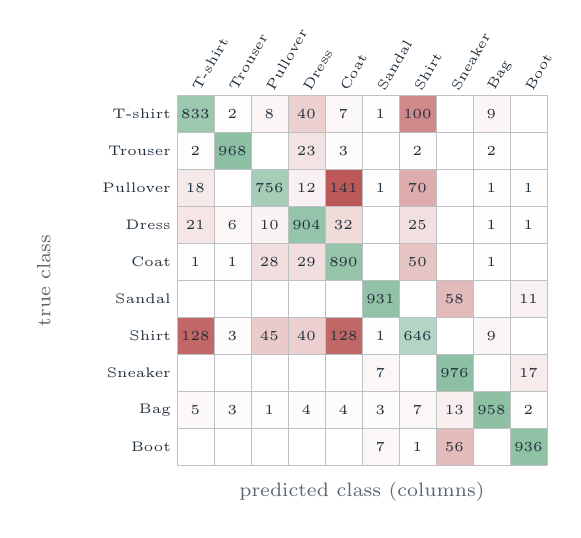
\begin{tikzpicture}[x=4.7mm,y=4.7mm,lab/.append style={font=\fontsize{5.2}{6}\selectfont}]
  \fill[cFfn!47] (0,0) rectangle ++(1,-1);
\node[lab] at (0.50,-0.50) {833};
\fill[cBad!1] (1,0) rectangle ++(1,-1);
\node[lab] at (1.50,-0.50) {2};
\fill[cBad!5] (2,0) rectangle ++(1,-1);
\node[lab] at (2.50,-0.50) {8};
\fill[cBad!24] (3,0) rectangle ++(1,-1);
\node[lab] at (3.50,-0.50) {40};
\fill[cBad!4] (4,0) rectangle ++(1,-1);
\node[lab] at (4.50,-0.50) {7};
\fill[cBad!1] (5,0) rectangle ++(1,-1);
\node[lab] at (5.50,-0.50) {1};
\fill[cBad!60] (6,0) rectangle ++(1,-1);
\node[lab] at (6.50,-0.50) {100};
\fill[cBad!5] (8,0) rectangle ++(1,-1);
\node[lab] at (8.50,-0.50) {9};
\node[lab,anchor=east] at (-0.15,-0.50) {T-shirt};
\node[lab,anchor=west,rotate=60] at (0.50,0.15) {T-shirt};
\fill[cBad!1] (0,-1) rectangle ++(1,-1);
\node[lab] at (0.50,-1.50) {2};
\fill[cFfn!55] (1,-1) rectangle ++(1,-1);
\node[lab] at (1.50,-1.50) {968};
\fill[cBad!14] (3,-1) rectangle ++(1,-1);
\node[lab] at (3.50,-1.50) {23};
\fill[cBad!2] (4,-1) rectangle ++(1,-1);
\node[lab] at (4.50,-1.50) {3};
\fill[cBad!1] (6,-1) rectangle ++(1,-1);
\node[lab] at (6.50,-1.50) {2};
\fill[cBad!1] (8,-1) rectangle ++(1,-1);
\node[lab] at (8.50,-1.50) {2};
\node[lab,anchor=east] at (-0.15,-1.50) {Trouser};
\node[lab,anchor=west,rotate=60] at (1.50,0.15) {Trouser};
\fill[cBad!11] (0,-2) rectangle ++(1,-1);
\node[lab] at (0.50,-2.50) {18};
\fill[cFfn!43] (2,-2) rectangle ++(1,-1);
\node[lab] at (2.50,-2.50) {756};
\fill[cBad!7] (3,-2) rectangle ++(1,-1);
\node[lab] at (3.50,-2.50) {12};
\fill[cBad!85] (4,-2) rectangle ++(1,-1);
\node[lab] at (4.50,-2.50) {141};
\fill[cBad!1] (5,-2) rectangle ++(1,-1);
\node[lab] at (5.50,-2.50) {1};
\fill[cBad!42] (6,-2) rectangle ++(1,-1);
\node[lab] at (6.50,-2.50) {70};
\fill[cBad!1] (8,-2) rectangle ++(1,-1);
\node[lab] at (8.50,-2.50) {1};
\fill[cBad!1] (9,-2) rectangle ++(1,-1);
\node[lab] at (9.50,-2.50) {1};
\node[lab,anchor=east] at (-0.15,-2.50) {Pullover};
\node[lab,anchor=west,rotate=60] at (2.50,0.15) {Pullover};
\fill[cBad!13] (0,-3) rectangle ++(1,-1);
\node[lab] at (0.50,-3.50) {21};
\fill[cBad!4] (1,-3) rectangle ++(1,-1);
\node[lab] at (1.50,-3.50) {6};
\fill[cBad!6] (2,-3) rectangle ++(1,-1);
\node[lab] at (2.50,-3.50) {10};
\fill[cFfn!51] (3,-3) rectangle ++(1,-1);
\node[lab] at (3.50,-3.50) {904};
\fill[cBad!19] (4,-3) rectangle ++(1,-1);
\node[lab] at (4.50,-3.50) {32};
\fill[cBad!15] (6,-3) rectangle ++(1,-1);
\node[lab] at (6.50,-3.50) {25};
\fill[cBad!1] (8,-3) rectangle ++(1,-1);
\node[lab] at (8.50,-3.50) {1};
\fill[cBad!1] (9,-3) rectangle ++(1,-1);
\node[lab] at (9.50,-3.50) {1};
\node[lab,anchor=east] at (-0.15,-3.50) {Dress};
\node[lab,anchor=west,rotate=60] at (3.50,0.15) {Dress};
\fill[cBad!1] (0,-4) rectangle ++(1,-1);
\node[lab] at (0.50,-4.50) {1};
\fill[cBad!1] (1,-4) rectangle ++(1,-1);
\node[lab] at (1.50,-4.50) {1};
\fill[cBad!17] (2,-4) rectangle ++(1,-1);
\node[lab] at (2.50,-4.50) {28};
\fill[cBad!17] (3,-4) rectangle ++(1,-1);
\node[lab] at (3.50,-4.50) {29};
\fill[cFfn!50] (4,-4) rectangle ++(1,-1);
\node[lab] at (4.50,-4.50) {890};
\fill[cBad!30] (6,-4) rectangle ++(1,-1);
\node[lab] at (6.50,-4.50) {50};
\fill[cBad!1] (8,-4) rectangle ++(1,-1);
\node[lab] at (8.50,-4.50) {1};
\node[lab,anchor=east] at (-0.15,-4.50) {Coat};
\node[lab,anchor=west,rotate=60] at (4.50,0.15) {Coat};
\fill[cFfn!52] (5,-5) rectangle ++(1,-1);
\node[lab] at (5.50,-5.50) {931};
\fill[cBad!35] (7,-5) rectangle ++(1,-1);
\node[lab] at (7.50,-5.50) {58};
\fill[cBad!7] (9,-5) rectangle ++(1,-1);
\node[lab] at (9.50,-5.50) {11};
\node[lab,anchor=east] at (-0.15,-5.50) {Sandal};
\node[lab,anchor=west,rotate=60] at (5.50,0.15) {Sandal};
\fill[cBad!77] (0,-6) rectangle ++(1,-1);
\node[lab] at (0.50,-6.50) {128};
\fill[cBad!2] (1,-6) rectangle ++(1,-1);
\node[lab] at (1.50,-6.50) {3};
\fill[cBad!27] (2,-6) rectangle ++(1,-1);
\node[lab] at (2.50,-6.50) {45};
\fill[cBad!24] (3,-6) rectangle ++(1,-1);
\node[lab] at (3.50,-6.50) {40};
\fill[cBad!77] (4,-6) rectangle ++(1,-1);
\node[lab] at (4.50,-6.50) {128};
\fill[cBad!1] (5,-6) rectangle ++(1,-1);
\node[lab] at (5.50,-6.50) {1};
\fill[cFfn!36] (6,-6) rectangle ++(1,-1);
\node[lab] at (6.50,-6.50) {646};
\fill[cBad!5] (8,-6) rectangle ++(1,-1);
\node[lab] at (8.50,-6.50) {9};
\node[lab,anchor=east] at (-0.15,-6.50) {Shirt};
\node[lab,anchor=west,rotate=60] at (6.50,0.15) {Shirt};
\fill[cBad!4] (5,-7) rectangle ++(1,-1);
\node[lab] at (5.50,-7.50) {7};
\fill[cFfn!55] (7,-7) rectangle ++(1,-1);
\node[lab] at (7.50,-7.50) {976};
\fill[cBad!10] (9,-7) rectangle ++(1,-1);
\node[lab] at (9.50,-7.50) {17};
\node[lab,anchor=east] at (-0.15,-7.50) {Sneaker};
\node[lab,anchor=west,rotate=60] at (7.50,0.15) {Sneaker};
\fill[cBad!3] (0,-8) rectangle ++(1,-1);
\node[lab] at (0.50,-8.50) {5};
\fill[cBad!2] (1,-8) rectangle ++(1,-1);
\node[lab] at (1.50,-8.50) {3};
\fill[cBad!1] (2,-8) rectangle ++(1,-1);
\node[lab] at (2.50,-8.50) {1};
\fill[cBad!2] (3,-8) rectangle ++(1,-1);
\node[lab] at (3.50,-8.50) {4};
\fill[cBad!2] (4,-8) rectangle ++(1,-1);
\node[lab] at (4.50,-8.50) {4};
\fill[cBad!2] (5,-8) rectangle ++(1,-1);
\node[lab] at (5.50,-8.50) {3};
\fill[cBad!4] (6,-8) rectangle ++(1,-1);
\node[lab] at (6.50,-8.50) {7};
\fill[cBad!8] (7,-8) rectangle ++(1,-1);
\node[lab] at (7.50,-8.50) {13};
\fill[cFfn!54] (8,-8) rectangle ++(1,-1);
\node[lab] at (8.50,-8.50) {958};
\fill[cBad!1] (9,-8) rectangle ++(1,-1);
\node[lab] at (9.50,-8.50) {2};
\node[lab,anchor=east] at (-0.15,-8.50) {Bag};
\node[lab,anchor=west,rotate=60] at (8.50,0.15) {Bag};
\fill[cBad!4] (5,-9) rectangle ++(1,-1);
\node[lab] at (5.50,-9.50) {7};
\fill[cBad!1] (6,-9) rectangle ++(1,-1);
\node[lab] at (6.50,-9.50) {1};
\fill[cBad!34] (7,-9) rectangle ++(1,-1);
\node[lab] at (7.50,-9.50) {56};
\fill[cFfn!53] (9,-9) rectangle ++(1,-1);
\node[lab] at (9.50,-9.50) {936};
\node[lab,anchor=east] at (-0.15,-9.50) {Boot};
\node[lab,anchor=west,rotate=60] at (9.50,0.15) {Boot};
\draw[cInk!30,line width=0.2pt,step=1] (0,0) grid (10,-10);

  \node[note,rotate=90] at (-3.6,-5) {true class};
  \node[note] at (5,-10.7) {predicted class (columns)};
\end{tikzpicture}

\vspace{0.3mm}
{\scriptsize\color{cTok}Confusion matrix, seed-0 CNN, \nTest{} test images (1{,}000 per class).}

\vspace{0.8mm}
\raggedright\footnotesize
\textbf{Where it fails.} Most confused pairs: \confOne{} (\confOneN{} errors), \confTwo{} (\confTwoN),
\confThree{} (\confThreeN). \upperShare\% of all errors are among the five upper-body garments.
Recall ranges from \worstRecall\% (\worstClass) to \bestRecall\% (\bestClass).
\end{columns}
\end{frame}

% ====================================================================== 18
\begin{frame}{What the network learned: first-layer filters and feature maps}
\begin{columns}[T,onlytextwidth]
\column{0.55\textwidth}
\centering
{\footnotesize\textbf{The 8 learned $5\times5$ kernels of conv1} \ (seed-0 CNN; {\color{cAtt}orange} $>0$, {\color{cEmb}blue} $<0$)}

\vspace{0.8mm}
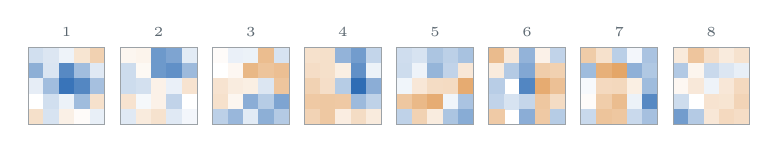
\begin{tikzpicture}[x=1.95mm,y=1.95mm,lab/.append style={font=\fontsize{5.5}{6}\selectfont,text=cTok}]
  \fill[cEmb!22] (0.00,0.00) rectangle ++(1.04,-1.04);
\fill[cEmb!17] (1.00,0.00) rectangle ++(1.04,-1.04);
\fill[cEmb!8] (2.00,0.00) rectangle ++(1.04,-1.04);
\fill[cAtt!21] (3.00,0.00) rectangle ++(1.04,-1.04);
\fill[cAtt!37] (4.00,0.00) rectangle ++(1.04,-1.04);
\fill[cEmb!55] (0.00,-1.00) rectangle ++(1.04,-1.04);
\fill[cEmb!18] (1.00,-1.00) rectangle ++(1.04,-1.04);
\fill[cEmb!81] (2.00,-1.00) rectangle ++(1.04,-1.04);
\fill[cEmb!45] (3.00,-1.00) rectangle ++(1.04,-1.04);
\fill[cEmb!15] (4.00,-1.00) rectangle ++(1.04,-1.04);
\fill[cEmb!12] (0.00,-2.00) rectangle ++(1.04,-1.04);
\fill[cEmb!45] (1.00,-2.00) rectangle ++(1.04,-1.04);
\fill[cEmb!95] (2.00,-2.00) rectangle ++(1.04,-1.04);
\fill[cEmb!82] (3.00,-2.00) rectangle ++(1.04,-1.04);
\fill[cEmb!43] (4.00,-2.00) rectangle ++(1.04,-1.04);
\fill[cEmb!22] (1.00,-3.00) rectangle ++(1.04,-1.04);
\fill[cEmb!9] (2.00,-3.00) rectangle ++(1.04,-1.04);
\fill[cEmb!46] (3.00,-3.00) rectangle ++(1.04,-1.04);
\fill[cAtt!24] (4.00,-3.00) rectangle ++(1.04,-1.04);
\fill[cAtt!25] (0.00,-4.00) rectangle ++(1.04,-1.04);
\fill[cEmb!19] (1.00,-4.00) rectangle ++(1.04,-1.04);
\fill[cAtt!12] (2.00,-4.00) rectangle ++(1.04,-1.04);
\fill[cAtt!3] (3.00,-4.00) rectangle ++(1.04,-1.04);
\fill[cEmb!11] (4.00,-4.00) rectangle ++(1.04,-1.04);
\draw[cInk!45,line width=0.3pt] (0.00,0.00) rectangle ++(5,-5);
\node[lab] at (2.50,1.00) {1};
\fill[cAtt!7] (6.00,0.00) rectangle ++(1.04,-1.04);
\fill[cAtt!9] (7.00,0.00) rectangle ++(1.04,-1.04);
\fill[cEmb!70] (8.00,0.00) rectangle ++(1.04,-1.04);
\fill[cEmb!62] (9.00,0.00) rectangle ++(1.04,-1.04);
\fill[cEmb!14] (10.00,0.00) rectangle ++(1.04,-1.04);
\fill[cEmb!24] (6.00,-1.00) rectangle ++(1.04,-1.04);
\fill[cAtt!5] (7.00,-1.00) rectangle ++(1.04,-1.04);
\fill[cEmb!70] (8.00,-1.00) rectangle ++(1.04,-1.04);
\fill[cEmb!76] (9.00,-1.00) rectangle ++(1.04,-1.04);
\fill[cEmb!47] (10.00,-1.00) rectangle ++(1.04,-1.04);
\fill[cEmb!24] (6.00,-2.00) rectangle ++(1.04,-1.04);
\fill[cEmb!21] (7.00,-2.00) rectangle ++(1.04,-1.04);
\fill[cAtt!11] (8.00,-2.00) rectangle ++(1.04,-1.04);
\fill[cEmb!10] (9.00,-2.00) rectangle ++(1.04,-1.04);
\fill[cAtt!22] (10.00,-2.00) rectangle ++(1.04,-1.04);
\fill[cAtt!22] (6.00,-3.00) rectangle ++(1.04,-1.04);
\fill[cEmb!5] (7.00,-3.00) rectangle ++(1.04,-1.04);
\fill[cAtt!11] (8.00,-3.00) rectangle ++(1.04,-1.04);
\fill[cEmb!30] (9.00,-3.00) rectangle ++(1.04,-1.04);
\fill[cEmb!15] (6.00,-4.00) rectangle ++(1.04,-1.04);
\fill[cAtt!16] (7.00,-4.00) rectangle ++(1.04,-1.04);
\fill[cAtt!23] (8.00,-4.00) rectangle ++(1.04,-1.04);
\fill[cEmb!15] (9.00,-4.00) rectangle ++(1.04,-1.04);
\fill[cEmb!6] (10.00,-4.00) rectangle ++(1.04,-1.04);
\draw[cInk!45,line width=0.3pt] (6.00,0.00) rectangle ++(5,-5);
\node[lab] at (8.50,1.00) {2};
\fill[cAtt!3] (12.00,0.00) rectangle ++(1.04,-1.04);
\fill[cEmb!10] (13.00,0.00) rectangle ++(1.04,-1.04);
\fill[cEmb!9] (14.00,0.00) rectangle ++(1.04,-1.04);
\fill[cAtt!53] (15.00,0.00) rectangle ++(1.04,-1.04);
\fill[cEmb!19] (16.00,0.00) rectangle ++(1.04,-1.04);
\fill[cAtt!6] (13.00,-1.00) rectangle ++(1.04,-1.04);
\fill[cAtt!57] (14.00,-1.00) rectangle ++(1.04,-1.04);
\fill[cAtt!47] (15.00,-1.00) rectangle ++(1.04,-1.04);
\fill[cAtt!51] (16.00,-1.00) rectangle ++(1.04,-1.04);
\fill[cAtt!22] (12.00,-2.00) rectangle ++(1.04,-1.04);
\fill[cAtt!15] (13.00,-2.00) rectangle ++(1.04,-1.04);
\fill[cAtt!13] (14.00,-2.00) rectangle ++(1.04,-1.04);
\fill[cEmb!17] (15.00,-2.00) rectangle ++(1.04,-1.04);
\fill[cAtt!46] (16.00,-2.00) rectangle ++(1.04,-1.04);
\fill[cAtt!24] (12.00,-3.00) rectangle ++(1.04,-1.04);
\fill[cAtt!7] (13.00,-3.00) rectangle ++(1.04,-1.04);
\fill[cEmb!56] (14.00,-3.00) rectangle ++(1.04,-1.04);
\fill[cEmb!35] (15.00,-3.00) rectangle ++(1.04,-1.04);
\fill[cEmb!62] (16.00,-3.00) rectangle ++(1.04,-1.04);
\fill[cEmb!32] (12.00,-4.00) rectangle ++(1.04,-1.04);
\fill[cEmb!49] (13.00,-4.00) rectangle ++(1.04,-1.04);
\fill[cEmb!14] (14.00,-4.00) rectangle ++(1.04,-1.04);
\fill[cEmb!55] (15.00,-4.00) rectangle ++(1.04,-1.04);
\fill[cEmb!36] (16.00,-4.00) rectangle ++(1.04,-1.04);
\draw[cInk!45,line width=0.3pt] (12.00,0.00) rectangle ++(5,-5);
\node[lab] at (14.50,1.00) {3};
\fill[cAtt!24] (18.00,0.00) rectangle ++(1.04,-1.04);
\fill[cAtt!25] (19.00,0.00) rectangle ++(1.04,-1.04);
\fill[cEmb!52] (20.00,0.00) rectangle ++(1.04,-1.04);
\fill[cEmb!68] (21.00,0.00) rectangle ++(1.04,-1.04);
\fill[cEmb!29] (22.00,0.00) rectangle ++(1.04,-1.04);
\fill[cAtt!27] (18.00,-1.00) rectangle ++(1.04,-1.04);
\fill[cAtt!25] (19.00,-1.00) rectangle ++(1.04,-1.04);
\fill[cAtt!13] (20.00,-1.00) rectangle ++(1.04,-1.04);
\fill[cEmb!76] (21.00,-1.00) rectangle ++(1.04,-1.04);
\fill[cEmb!9] (22.00,-1.00) rectangle ++(1.04,-1.04);
\fill[cAtt!36] (18.00,-2.00) rectangle ++(1.04,-1.04);
\fill[cAtt!26] (19.00,-2.00) rectangle ++(1.04,-1.04);
\fill[cEmb!35] (20.00,-2.00) rectangle ++(1.04,-1.04);
\fill[cEmb!100] (21.00,-2.00) rectangle ++(1.04,-1.04);
\fill[cEmb!56] (22.00,-2.00) rectangle ++(1.04,-1.04);
\fill[cAtt!43] (18.00,-3.00) rectangle ++(1.04,-1.04);
\fill[cAtt!44] (19.00,-3.00) rectangle ++(1.04,-1.04);
\fill[cAtt!43] (20.00,-3.00) rectangle ++(1.04,-1.04);
\fill[cEmb!47] (21.00,-3.00) rectangle ++(1.04,-1.04);
\fill[cEmb!31] (22.00,-3.00) rectangle ++(1.04,-1.04);
\fill[cAtt!35] (18.00,-4.00) rectangle ++(1.04,-1.04);
\fill[cAtt!44] (19.00,-4.00) rectangle ++(1.04,-1.04);
\fill[cAtt!14] (20.00,-4.00) rectangle ++(1.04,-1.04);
\fill[cAtt!28] (21.00,-4.00) rectangle ++(1.04,-1.04);
\fill[cAtt!16] (22.00,-4.00) rectangle ++(1.04,-1.04);
\draw[cInk!45,line width=0.3pt] (18.00,0.00) rectangle ++(5,-5);
\node[lab] at (20.50,1.00) {4};
\fill[cEmb!23] (24.00,0.00) rectangle ++(1.04,-1.04);
\fill[cEmb!19] (25.00,0.00) rectangle ++(1.04,-1.04);
\fill[cEmb!40] (26.00,0.00) rectangle ++(1.04,-1.04);
\fill[cEmb!32] (27.00,0.00) rectangle ++(1.04,-1.04);
\fill[cEmb!42] (28.00,0.00) rectangle ++(1.04,-1.04);
\fill[cEmb!24] (24.00,-1.00) rectangle ++(1.04,-1.04);
\fill[cEmb!8] (25.00,-1.00) rectangle ++(1.04,-1.04);
\fill[cEmb!51] (26.00,-1.00) rectangle ++(1.04,-1.04);
\fill[cEmb!30] (27.00,-1.00) rectangle ++(1.04,-1.04);
\fill[cAtt!19] (28.00,-1.00) rectangle ++(1.04,-1.04);
\fill[cEmb!7] (24.00,-2.00) rectangle ++(1.04,-1.04);
\fill[cAtt!19] (25.00,-2.00) rectangle ++(1.04,-1.04);
\fill[cAtt!28] (26.00,-2.00) rectangle ++(1.04,-1.04);
\fill[cAtt!29] (27.00,-2.00) rectangle ++(1.04,-1.04);
\fill[cAtt!67] (28.00,-2.00) rectangle ++(1.04,-1.04);
\fill[cAtt!45] (24.00,-3.00) rectangle ++(1.04,-1.04);
\fill[cAtt!56] (25.00,-3.00) rectangle ++(1.04,-1.04);
\fill[cAtt!66] (26.00,-3.00) rectangle ++(1.04,-1.04);
\fill[cEmb!7] (27.00,-3.00) rectangle ++(1.04,-1.04);
\fill[cEmb!41] (28.00,-3.00) rectangle ++(1.04,-1.04);
\fill[cEmb!31] (24.00,-4.00) rectangle ++(1.04,-1.04);
\fill[cAtt!36] (25.00,-4.00) rectangle ++(1.04,-1.04);
\fill[cAtt!15] (26.00,-4.00) rectangle ++(1.04,-1.04);
\fill[cEmb!40] (27.00,-4.00) rectangle ++(1.04,-1.04);
\fill[cEmb!57] (28.00,-4.00) rectangle ++(1.04,-1.04);
\draw[cInk!45,line width=0.3pt] (24.00,0.00) rectangle ++(5,-5);
\node[lab] at (26.50,1.00) {5};
\fill[cAtt!54] (30.00,0.00) rectangle ++(1.04,-1.04);
\fill[cAtt!18] (31.00,0.00) rectangle ++(1.04,-1.04);
\fill[cEmb!52] (32.00,0.00) rectangle ++(1.04,-1.04);
\fill[cAtt!11] (33.00,0.00) rectangle ++(1.04,-1.04);
\fill[cEmb!30] (34.00,0.00) rectangle ++(1.04,-1.04);
\fill[cAtt!16] (30.00,-1.00) rectangle ++(1.04,-1.04);
\fill[cEmb!36] (31.00,-1.00) rectangle ++(1.04,-1.04);
\fill[cEmb!60] (32.00,-1.00) rectangle ++(1.04,-1.04);
\fill[cAtt!40] (33.00,-1.00) rectangle ++(1.04,-1.04);
\fill[cAtt!37] (34.00,-1.00) rectangle ++(1.04,-1.04);
\fill[cEmb!34] (30.00,-2.00) rectangle ++(1.04,-1.04);
\fill[cEmb!83] (32.00,-2.00) rectangle ++(1.04,-1.04);
\fill[cAtt!67] (33.00,-2.00) rectangle ++(1.04,-1.04);
\fill[cAtt!50] (34.00,-2.00) rectangle ++(1.04,-1.04);
\fill[cEmb!30] (30.00,-3.00) rectangle ++(1.04,-1.04);
\fill[cEmb!19] (31.00,-3.00) rectangle ++(1.04,-1.04);
\fill[cEmb!28] (32.00,-3.00) rectangle ++(1.04,-1.04);
\fill[cAtt!45] (33.00,-3.00) rectangle ++(1.04,-1.04);
\fill[cAtt!28] (34.00,-3.00) rectangle ++(1.04,-1.04);
\fill[cAtt!42] (30.00,-4.00) rectangle ++(1.04,-1.04);
\fill[cEmb!56] (32.00,-4.00) rectangle ++(1.04,-1.04);
\fill[cAtt!43] (33.00,-4.00) rectangle ++(1.04,-1.04);
\fill[cEmb!35] (34.00,-4.00) rectangle ++(1.04,-1.04);
\draw[cInk!45,line width=0.3pt] (30.00,0.00) rectangle ++(5,-5);
\node[lab] at (32.50,1.00) {6};
\fill[cAtt!41] (36.00,0.00) rectangle ++(1.04,-1.04);
\fill[cAtt!24] (37.00,0.00) rectangle ++(1.04,-1.04);
\fill[cEmb!33] (38.00,0.00) rectangle ++(1.04,-1.04);
\fill[cEmb!6] (39.00,0.00) rectangle ++(1.04,-1.04);
\fill[cEmb!41] (40.00,0.00) rectangle ++(1.04,-1.04);
\fill[cEmb!46] (36.00,-1.00) rectangle ++(1.04,-1.04);
\fill[cAtt!63] (37.00,-1.00) rectangle ++(1.04,-1.04);
\fill[cAtt!71] (38.00,-1.00) rectangle ++(1.04,-1.04);
\fill[cEmb!54] (39.00,-1.00) rectangle ++(1.04,-1.04);
\fill[cEmb!38] (40.00,-1.00) rectangle ++(1.04,-1.04);
\fill[cEmb!4] (36.00,-2.00) rectangle ++(1.04,-1.04);
\fill[cAtt!30] (37.00,-2.00) rectangle ++(1.04,-1.04);
\fill[cAtt!31] (38.00,-2.00) rectangle ++(1.04,-1.04);
\fill[cAtt!13] (39.00,-2.00) rectangle ++(1.04,-1.04);
\fill[cEmb!46] (40.00,-2.00) rectangle ++(1.04,-1.04);
\fill[cAtt!3] (36.00,-3.00) rectangle ++(1.04,-1.04);
\fill[cAtt!40] (37.00,-3.00) rectangle ++(1.04,-1.04);
\fill[cAtt!53] (38.00,-3.00) rectangle ++(1.04,-1.04);
\fill[cEmb!9] (39.00,-3.00) rectangle ++(1.04,-1.04);
\fill[cEmb!81] (40.00,-3.00) rectangle ++(1.04,-1.04);
\fill[cEmb!26] (36.00,-4.00) rectangle ++(1.04,-1.04);
\fill[cAtt!47] (37.00,-4.00) rectangle ++(1.04,-1.04);
\fill[cAtt!45] (38.00,-4.00) rectangle ++(1.04,-1.04);
\fill[cEmb!26] (39.00,-4.00) rectangle ++(1.04,-1.04);
\fill[cEmb!43] (40.00,-4.00) rectangle ++(1.04,-1.04);
\draw[cInk!45,line width=0.3pt] (36.00,0.00) rectangle ++(5,-5);
\node[lab] at (38.50,1.00) {7};
\fill[cAtt!17] (42.00,0.00) rectangle ++(1.04,-1.04);
\fill[cAtt!46] (43.00,0.00) rectangle ++(1.04,-1.04);
\fill[cAtt!26] (44.00,0.00) rectangle ++(1.04,-1.04);
\fill[cAtt!16] (45.00,0.00) rectangle ++(1.04,-1.04);
\fill[cAtt!23] (46.00,0.00) rectangle ++(1.04,-1.04);
\fill[cEmb!37] (42.00,-1.00) rectangle ++(1.04,-1.04);
\fill[cAtt!8] (43.00,-1.00) rectangle ++(1.04,-1.04);
\fill[cEmb!26] (44.00,-1.00) rectangle ++(1.04,-1.04);
\fill[cEmb!17] (45.00,-1.00) rectangle ++(1.04,-1.04);
\fill[cEmb!11] (46.00,-1.00) rectangle ++(1.04,-1.04);
\fill[cAtt!6] (42.00,-2.00) rectangle ++(1.04,-1.04);
\fill[cAtt!18] (43.00,-2.00) rectangle ++(1.04,-1.04);
\fill[cEmb!8] (44.00,-2.00) rectangle ++(1.04,-1.04);
\fill[cAtt!19] (45.00,-2.00) rectangle ++(1.04,-1.04);
\fill[cAtt!30] (46.00,-2.00) rectangle ++(1.04,-1.04);
\fill[cEmb!24] (42.00,-3.00) rectangle ++(1.04,-1.04);
\fill[cAtt!22] (44.00,-3.00) rectangle ++(1.04,-1.04);
\fill[cAtt!21] (45.00,-3.00) rectangle ++(1.04,-1.04);
\fill[cAtt!34] (46.00,-3.00) rectangle ++(1.04,-1.04);
\fill[cEmb!68] (42.00,-4.00) rectangle ++(1.04,-1.04);
\fill[cEmb!36] (43.00,-4.00) rectangle ++(1.04,-1.04);
\fill[cAtt!19] (44.00,-4.00) rectangle ++(1.04,-1.04);
\fill[cAtt!30] (45.00,-4.00) rectangle ++(1.04,-1.04);
\fill[cAtt!27] (46.00,-4.00) rectangle ++(1.04,-1.04);
\draw[cInk!45,line width=0.3pt] (42.00,0.00) rectangle ++(5,-5);
\node[lab] at (44.50,1.00) {8};

\end{tikzpicture}

\vspace{1.5mm}
{\footnotesize\textbf{Their feature maps for test image 0, after ReLU} \ (darker = larger)}

\vspace{0.8mm}
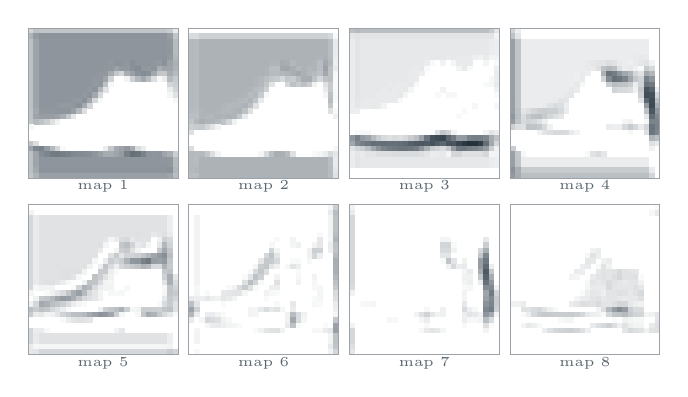
\begin{tikzpicture}[x=0.68mm,y=0.68mm,lab/.append style={font=\fontsize{5.5}{6}\selectfont,text=cTok}]
  \fill[cInk!20] (0.00,0.00) rectangle ++(1.04,-1.04);
\fill[cInk!29] (1.00,0.00) rectangle ++(1.04,-1.04);
\fill[cInk!28] (2.00,0.00) rectangle ++(24.04,-1.04);
\fill[cInk!24] (26.00,0.00) rectangle ++(1.04,-1.04);
\fill[cInk!10] (27.00,0.00) rectangle ++(1.04,-1.04);
\fill[cInk!36] (0.00,-1.00) rectangle ++(1.04,-1.04);
\fill[cInk!48] (1.00,-1.00) rectangle ++(1.04,-1.04);
\fill[cInk!52] (2.00,-1.00) rectangle ++(24.04,-1.04);
\fill[cInk!47] (26.00,-1.00) rectangle ++(1.04,-1.04);
\fill[cInk!28] (27.00,-1.00) rectangle ++(1.04,-1.04);
\fill[cInk!30] (0.00,-2.00) rectangle ++(1.04,-1.04);
\fill[cInk!44] (1.00,-2.00) rectangle ++(1.04,-1.04);
\fill[cInk!51] (2.00,-2.00) rectangle ++(24.04,-1.04);
\fill[cInk!50] (26.00,-2.00) rectangle ++(1.04,-1.04);
\fill[cInk!33] (27.00,-2.00) rectangle ++(1.04,-1.04);
\fill[cInk!30] (0.00,-3.00) rectangle ++(1.04,-1.04);
\fill[cInk!44] (1.00,-3.00) rectangle ++(1.04,-1.04);
\fill[cInk!51] (2.00,-3.00) rectangle ++(24.04,-1.04);
\fill[cInk!50] (26.00,-3.00) rectangle ++(1.04,-1.04);
\fill[cInk!33] (27.00,-3.00) rectangle ++(1.04,-1.04);
\fill[cInk!30] (0.00,-4.00) rectangle ++(1.04,-1.04);
\fill[cInk!44] (1.00,-4.00) rectangle ++(1.04,-1.04);
\fill[cInk!51] (2.00,-4.00) rectangle ++(24.04,-1.04);
\fill[cInk!50] (26.00,-4.00) rectangle ++(1.04,-1.04);
\fill[cInk!33] (27.00,-4.00) rectangle ++(1.04,-1.04);
\fill[cInk!30] (0.00,-5.00) rectangle ++(1.04,-1.04);
\fill[cInk!44] (1.00,-5.00) rectangle ++(1.04,-1.04);
\fill[cInk!51] (2.00,-5.00) rectangle ++(23.04,-1.04);
\fill[cInk!52] (25.00,-5.00) rectangle ++(1.04,-1.04);
\fill[cInk!49] (26.00,-5.00) rectangle ++(1.04,-1.04);
\fill[cInk!35] (27.00,-5.00) rectangle ++(1.04,-1.04);
\fill[cInk!30] (0.00,-6.00) rectangle ++(1.04,-1.04);
\fill[cInk!44] (1.00,-6.00) rectangle ++(1.04,-1.04);
\fill[cInk!51] (2.00,-6.00) rectangle ++(13.04,-1.04);
\fill[cInk!50] (15.00,-6.00) rectangle ++(1.04,-1.04);
\fill[cInk!52] (16.00,-6.00) rectangle ++(2.04,-1.04);
\fill[cInk!50] (18.00,-6.00) rectangle ++(1.04,-1.04);
\fill[cInk!54] (19.00,-6.00) rectangle ++(1.04,-1.04);
\fill[cInk!51] (20.00,-6.00) rectangle ++(3.04,-1.04);
\fill[cInk!50] (23.00,-6.00) rectangle ++(1.04,-1.04);
\fill[cInk!49] (24.00,-6.00) rectangle ++(1.04,-1.04);
\fill[cInk!53] (25.00,-6.00) rectangle ++(1.04,-1.04);
\fill[cInk!45] (26.00,-6.00) rectangle ++(1.04,-1.04);
\fill[cInk!38] (27.00,-6.00) rectangle ++(1.04,-1.04);
\fill[cInk!30] (0.00,-7.00) rectangle ++(1.04,-1.04);
\fill[cInk!44] (1.00,-7.00) rectangle ++(1.04,-1.04);
\fill[cInk!51] (2.00,-7.00) rectangle ++(12.04,-1.04);
\fill[cInk!50] (14.00,-7.00) rectangle ++(2.04,-1.04);
\fill[cInk!45] (16.00,-7.00) rectangle ++(1.04,-1.04);
\fill[cInk!49] (17.00,-7.00) rectangle ++(2.04,-1.04);
\fill[cInk!53] (19.00,-7.00) rectangle ++(1.04,-1.04);
\fill[cInk!55] (20.00,-7.00) rectangle ++(1.04,-1.04);
\fill[cInk!50] (21.00,-7.00) rectangle ++(1.04,-1.04);
\fill[cInk!49] (22.00,-7.00) rectangle ++(1.04,-1.04);
\fill[cInk!51] (23.00,-7.00) rectangle ++(1.04,-1.04);
\fill[cInk!39] (24.00,-7.00) rectangle ++(1.04,-1.04);
\fill[cInk!44] (25.00,-7.00) rectangle ++(2.04,-1.04);
\fill[cInk!37] (27.00,-7.00) rectangle ++(1.04,-1.04);
\fill[cInk!30] (0.00,-8.00) rectangle ++(1.04,-1.04);
\fill[cInk!44] (1.00,-8.00) rectangle ++(1.04,-1.04);
\fill[cInk!51] (2.00,-8.00) rectangle ++(11.04,-1.04);
\fill[cInk!50] (13.00,-8.00) rectangle ++(2.04,-1.04);
\fill[cInk!40] (15.00,-8.00) rectangle ++(1.04,-1.04);
\fill[cInk!27] (16.00,-8.00) rectangle ++(1.04,-1.04);
\fill[cInk!20] (17.00,-8.00) rectangle ++(1.04,-1.04);
\fill[cInk!39] (18.00,-8.00) rectangle ++(1.04,-1.04);
\fill[cInk!46] (19.00,-8.00) rectangle ++(1.04,-1.04);
\fill[cInk!53] (20.00,-8.00) rectangle ++(1.04,-1.04);
\fill[cInk!55] (21.00,-8.00) rectangle ++(1.04,-1.04);
\fill[cInk!54] (22.00,-8.00) rectangle ++(1.04,-1.04);
\fill[cInk!42] (23.00,-8.00) rectangle ++(1.04,-1.04);
\fill[cInk!28] (24.00,-8.00) rectangle ++(1.04,-1.04);
\fill[cInk!27] (25.00,-8.00) rectangle ++(1.04,-1.04);
\fill[cInk!40] (26.00,-8.00) rectangle ++(1.04,-1.04);
\fill[cInk!33] (27.00,-8.00) rectangle ++(1.04,-1.04);
\fill[cInk!30] (0.00,-9.00) rectangle ++(1.04,-1.04);
\fill[cInk!44] (1.00,-9.00) rectangle ++(1.04,-1.04);
\fill[cInk!51] (2.00,-9.00) rectangle ++(10.04,-1.04);
\fill[cInk!50] (12.00,-9.00) rectangle ++(2.04,-1.04);
\fill[cInk!44] (14.00,-9.00) rectangle ++(1.04,-1.04);
\fill[cInk!21] (15.00,-9.00) rectangle ++(1.04,-1.04);
\fill[cInk!6] (18.00,-9.00) rectangle ++(1.04,-1.04);
\fill[cInk!22] (19.00,-9.00) rectangle ++(1.04,-1.04);
\fill[cInk!34] (20.00,-9.00) rectangle ++(1.04,-1.04);
\fill[cInk!42] (21.00,-9.00) rectangle ++(1.04,-1.04);
\fill[cInk!32] (22.00,-9.00) rectangle ++(1.04,-1.04);
\fill[cInk!16] (23.00,-9.00) rectangle ++(1.04,-1.04);
\fill[cInk!3] (24.00,-9.00) rectangle ++(1.04,-1.04);
\fill[cInk!9] (25.00,-9.00) rectangle ++(1.04,-1.04);
\fill[cInk!33] (26.00,-9.00) rectangle ++(1.04,-1.04);
\fill[cInk!25] (27.00,-9.00) rectangle ++(1.04,-1.04);
\fill[cInk!30] (0.00,-10.00) rectangle ++(1.04,-1.04);
\fill[cInk!44] (1.00,-10.00) rectangle ++(1.04,-1.04);
\fill[cInk!51] (2.00,-10.00) rectangle ++(10.04,-1.04);
\fill[cInk!49] (12.00,-10.00) rectangle ++(1.04,-1.04);
\fill[cInk!50] (13.00,-10.00) rectangle ++(1.04,-1.04);
\fill[cInk!30] (14.00,-10.00) rectangle ++(1.04,-1.04);
\fill[cInk!4] (15.00,-10.00) rectangle ++(1.04,-1.04);
\fill[cInk!20] (26.00,-10.00) rectangle ++(1.04,-1.04);
\fill[cInk!23] (27.00,-10.00) rectangle ++(1.04,-1.04);
\fill[cInk!30] (0.00,-11.00) rectangle ++(1.04,-1.04);
\fill[cInk!44] (1.00,-11.00) rectangle ++(1.04,-1.04);
\fill[cInk!51] (2.00,-11.00) rectangle ++(9.04,-1.04);
\fill[cInk!49] (11.00,-11.00) rectangle ++(1.04,-1.04);
\fill[cInk!52] (12.00,-11.00) rectangle ++(1.04,-1.04);
\fill[cInk!35] (13.00,-11.00) rectangle ++(1.04,-1.04);
\fill[cInk!14] (14.00,-11.00) rectangle ++(1.04,-1.04);
\fill[cInk!9] (26.00,-11.00) rectangle ++(1.04,-1.04);
\fill[cInk!20] (27.00,-11.00) rectangle ++(1.04,-1.04);
\fill[cInk!30] (0.00,-12.00) rectangle ++(1.04,-1.04);
\fill[cInk!44] (1.00,-12.00) rectangle ++(1.04,-1.04);
\fill[cInk!51] (2.00,-12.00) rectangle ++(8.04,-1.04);
\fill[cInk!49] (10.00,-12.00) rectangle ++(1.04,-1.04);
\fill[cInk!52] (11.00,-12.00) rectangle ++(1.04,-1.04);
\fill[cInk!42] (12.00,-12.00) rectangle ++(1.04,-1.04);
\fill[cInk!18] (13.00,-12.00) rectangle ++(1.04,-1.04);
\fill[cInk!5] (26.00,-12.00) rectangle ++(1.04,-1.04);
\fill[cInk!14] (27.00,-12.00) rectangle ++(1.04,-1.04);
\fill[cInk!30] (0.00,-13.00) rectangle ++(1.04,-1.04);
\fill[cInk!44] (1.00,-13.00) rectangle ++(1.04,-1.04);
\fill[cInk!51] (2.00,-13.00) rectangle ++(6.04,-1.04);
\fill[cInk!50] (8.00,-13.00) rectangle ++(1.04,-1.04);
\fill[cInk!49] (9.00,-13.00) rectangle ++(1.04,-1.04);
\fill[cInk!53] (10.00,-13.00) rectangle ++(1.04,-1.04);
\fill[cInk!43] (11.00,-13.00) rectangle ++(1.04,-1.04);
\fill[cInk!19] (12.00,-13.00) rectangle ++(1.04,-1.04);
\fill[cInk!3] (13.00,-13.00) rectangle ++(1.04,-1.04);
\fill[cInk!4] (27.00,-13.00) rectangle ++(1.04,-1.04);
\fill[cInk!30] (0.00,-14.00) rectangle ++(1.04,-1.04);
\fill[cInk!44] (1.00,-14.00) rectangle ++(1.04,-1.04);
\fill[cInk!51] (2.00,-14.00) rectangle ++(3.04,-1.04);
\fill[cInk!50] (5.00,-14.00) rectangle ++(1.04,-1.04);
\fill[cInk!49] (6.00,-14.00) rectangle ++(2.04,-1.04);
\fill[cInk!50] (8.00,-14.00) rectangle ++(1.04,-1.04);
\fill[cInk!53] (9.00,-14.00) rectangle ++(1.04,-1.04);
\fill[cInk!41] (10.00,-14.00) rectangle ++(1.04,-1.04);
\fill[cInk!20] (11.00,-14.00) rectangle ++(1.04,-1.04);
\fill[cInk!29] (0.00,-15.00) rectangle ++(1.04,-1.04);
\fill[cInk!42] (1.00,-15.00) rectangle ++(1.04,-1.04);
\fill[cInk!50] (2.00,-15.00) rectangle ++(3.04,-1.04);
\fill[cInk!51] (5.00,-15.00) rectangle ++(3.04,-1.04);
\fill[cInk!46] (8.00,-15.00) rectangle ++(1.04,-1.04);
\fill[cInk!34] (9.00,-15.00) rectangle ++(1.04,-1.04);
\fill[cInk!16] (10.00,-15.00) rectangle ++(1.04,-1.04);
\fill[cInk!29] (0.00,-16.00) rectangle ++(1.04,-1.04);
\fill[cInk!44] (1.00,-16.00) rectangle ++(1.04,-1.04);
\fill[cInk!47] (2.00,-16.00) rectangle ++(3.04,-1.04);
\fill[cInk!45] (5.00,-16.00) rectangle ++(1.04,-1.04);
\fill[cInk!39] (6.00,-16.00) rectangle ++(1.04,-1.04);
\fill[cInk!27] (7.00,-16.00) rectangle ++(1.04,-1.04);
\fill[cInk!12] (8.00,-16.00) rectangle ++(1.04,-1.04);
\fill[cInk!27] (0.00,-17.00) rectangle ++(1.04,-1.04);
\fill[cInk!33] (1.00,-17.00) rectangle ++(1.04,-1.04);
\fill[cInk!29] (2.00,-17.00) rectangle ++(1.04,-1.04);
\fill[cInk!23] (3.00,-17.00) rectangle ++(1.04,-1.04);
\fill[cInk!15] (4.00,-17.00) rectangle ++(1.04,-1.04);
\fill[cInk!7] (5.00,-17.00) rectangle ++(1.04,-1.04);
\fill[cInk!4] (0.00,-18.00) rectangle ++(1.04,-1.04);
\fill[cInk!27] (0.00,-21.00) rectangle ++(1.04,-1.04);
\fill[cInk!16] (1.00,-21.00) rectangle ++(1.04,-1.04);
\fill[cInk!44] (0.00,-22.00) rectangle ++(1.04,-1.04);
\fill[cInk!58] (1.00,-22.00) rectangle ++(1.04,-1.04);
\fill[cInk!60] (2.00,-22.00) rectangle ++(1.04,-1.04);
\fill[cInk!48] (3.00,-22.00) rectangle ++(1.04,-1.04);
\fill[cInk!34] (4.00,-22.00) rectangle ++(1.04,-1.04);
\fill[cInk!20] (5.00,-22.00) rectangle ++(1.04,-1.04);
\fill[cInk!3] (6.00,-22.00) rectangle ++(1.04,-1.04);
\fill[cInk!9] (14.00,-22.00) rectangle ++(1.04,-1.04);
\fill[cInk!27] (15.00,-22.00) rectangle ++(1.04,-1.04);
\fill[cInk!41] (16.00,-22.00) rectangle ++(1.04,-1.04);
\fill[cInk!45] (17.00,-22.00) rectangle ++(1.04,-1.04);
\fill[cInk!50] (18.00,-22.00) rectangle ++(1.04,-1.04);
\fill[cInk!40] (19.00,-22.00) rectangle ++(1.04,-1.04);
\fill[cInk!17] (20.00,-22.00) rectangle ++(1.04,-1.04);
\fill[cInk!9] (21.00,-22.00) rectangle ++(1.04,-1.04);
\fill[cInk!30] (0.00,-23.00) rectangle ++(1.04,-1.04);
\fill[cInk!44] (1.00,-23.00) rectangle ++(1.04,-1.04);
\fill[cInk!55] (2.00,-23.00) rectangle ++(1.04,-1.04);
\fill[cInk!59] (3.00,-23.00) rectangle ++(1.04,-1.04);
\fill[cInk!63] (4.00,-23.00) rectangle ++(1.04,-1.04);
\fill[cInk!64] (5.00,-23.00) rectangle ++(1.04,-1.04);
\fill[cInk!62] (6.00,-23.00) rectangle ++(1.04,-1.04);
\fill[cInk!60] (7.00,-23.00) rectangle ++(1.04,-1.04);
\fill[cInk!57] (8.00,-23.00) rectangle ++(1.04,-1.04);
\fill[cInk!56] (9.00,-23.00) rectangle ++(1.04,-1.04);
\fill[cInk!55] (10.00,-23.00) rectangle ++(1.04,-1.04);
\fill[cInk!54] (11.00,-23.00) rectangle ++(1.04,-1.04);
\fill[cInk!51] (12.00,-23.00) rectangle ++(1.04,-1.04);
\fill[cInk!46] (13.00,-23.00) rectangle ++(1.04,-1.04);
\fill[cInk!40] (14.00,-23.00) rectangle ++(2.04,-1.04);
\fill[cInk!44] (16.00,-23.00) rectangle ++(1.04,-1.04);
\fill[cInk!48] (17.00,-23.00) rectangle ++(1.04,-1.04);
\fill[cInk!61] (18.00,-23.00) rectangle ++(1.04,-1.04);
\fill[cInk!69] (19.00,-23.00) rectangle ++(1.04,-1.04);
\fill[cInk!67] (20.00,-23.00) rectangle ++(1.04,-1.04);
\fill[cInk!60] (21.00,-23.00) rectangle ++(1.04,-1.04);
\fill[cInk!52] (22.00,-23.00) rectangle ++(1.04,-1.04);
\fill[cInk!51] (23.00,-23.00) rectangle ++(1.04,-1.04);
\fill[cInk!52] (24.00,-23.00) rectangle ++(1.04,-1.04);
\fill[cInk!44] (25.00,-23.00) rectangle ++(1.04,-1.04);
\fill[cInk!39] (26.00,-23.00) rectangle ++(1.04,-1.04);
\fill[cInk!23] (27.00,-23.00) rectangle ++(1.04,-1.04);
\fill[cInk!30] (0.00,-24.00) rectangle ++(1.04,-1.04);
\fill[cInk!44] (1.00,-24.00) rectangle ++(1.04,-1.04);
\fill[cInk!51] (2.00,-24.00) rectangle ++(24.04,-1.04);
\fill[cInk!50] (26.00,-24.00) rectangle ++(1.04,-1.04);
\fill[cInk!33] (27.00,-24.00) rectangle ++(1.04,-1.04);
\fill[cInk!30] (0.00,-25.00) rectangle ++(1.04,-1.04);
\fill[cInk!44] (1.00,-25.00) rectangle ++(1.04,-1.04);
\fill[cInk!51] (2.00,-25.00) rectangle ++(24.04,-1.04);
\fill[cInk!50] (26.00,-25.00) rectangle ++(1.04,-1.04);
\fill[cInk!33] (27.00,-25.00) rectangle ++(1.04,-1.04);
\fill[cInk!30] (0.00,-26.00) rectangle ++(1.04,-1.04);
\fill[cInk!42] (1.00,-26.00) rectangle ++(1.04,-1.04);
\fill[cInk!52] (2.00,-26.00) rectangle ++(24.04,-1.04);
\fill[cInk!53] (26.00,-26.00) rectangle ++(1.04,-1.04);
\fill[cInk!35] (27.00,-26.00) rectangle ++(1.04,-1.04);
\fill[cInk!27] (0.00,-27.00) rectangle ++(1.04,-1.04);
\fill[cInk!36] (1.00,-27.00) rectangle ++(1.04,-1.04);
\fill[cInk!46] (2.00,-27.00) rectangle ++(24.04,-1.04);
\fill[cInk!44] (26.00,-27.00) rectangle ++(1.04,-1.04);
\fill[cInk!32] (27.00,-27.00) rectangle ++(1.04,-1.04);
\draw[cInk!45,line width=0.3pt] (0.00,0.00) rectangle ++(28,-28);
\node[lab] at (14.00,-29.60) {map 1};
\fill[cInk!17] (30.00,-1.00) rectangle ++(2.04,-1.04);
\fill[cInk!22] (32.00,-1.00) rectangle ++(24.04,-1.04);
\fill[cInk!19] (56.00,-1.00) rectangle ++(1.04,-1.04);
\fill[cInk!3] (57.00,-1.00) rectangle ++(1.04,-1.04);
\fill[cInk!34] (30.00,-2.00) rectangle ++(1.04,-1.04);
\fill[cInk!33] (31.00,-2.00) rectangle ++(1.04,-1.04);
\fill[cInk!37] (32.00,-2.00) rectangle ++(24.04,-1.04);
\fill[cInk!32] (56.00,-2.00) rectangle ++(1.04,-1.04);
\fill[cInk!10] (57.00,-2.00) rectangle ++(1.04,-1.04);
\fill[cInk!34] (30.00,-3.00) rectangle ++(1.04,-1.04);
\fill[cInk!33] (31.00,-3.00) rectangle ++(1.04,-1.04);
\fill[cInk!37] (32.00,-3.00) rectangle ++(24.04,-1.04);
\fill[cInk!32] (56.00,-3.00) rectangle ++(1.04,-1.04);
\fill[cInk!10] (57.00,-3.00) rectangle ++(1.04,-1.04);
\fill[cInk!34] (30.00,-4.00) rectangle ++(1.04,-1.04);
\fill[cInk!33] (31.00,-4.00) rectangle ++(1.04,-1.04);
\fill[cInk!37] (32.00,-4.00) rectangle ++(24.04,-1.04);
\fill[cInk!32] (56.00,-4.00) rectangle ++(1.04,-1.04);
\fill[cInk!10] (57.00,-4.00) rectangle ++(1.04,-1.04);
\fill[cInk!34] (30.00,-5.00) rectangle ++(1.04,-1.04);
\fill[cInk!33] (31.00,-5.00) rectangle ++(1.04,-1.04);
\fill[cInk!37] (32.00,-5.00) rectangle ++(22.04,-1.04);
\fill[cInk!36] (54.00,-5.00) rectangle ++(1.04,-1.04);
\fill[cInk!38] (55.00,-5.00) rectangle ++(1.04,-1.04);
\fill[cInk!33] (56.00,-5.00) rectangle ++(1.04,-1.04);
\fill[cInk!9] (57.00,-5.00) rectangle ++(1.04,-1.04);
\fill[cInk!34] (30.00,-6.00) rectangle ++(1.04,-1.04);
\fill[cInk!33] (31.00,-6.00) rectangle ++(1.04,-1.04);
\fill[cInk!37] (32.00,-6.00) rectangle ++(13.04,-1.04);
\fill[cInk!36] (45.00,-6.00) rectangle ++(2.04,-1.04);
\fill[cInk!40] (47.00,-6.00) rectangle ++(1.04,-1.04);
\fill[cInk!39] (48.00,-6.00) rectangle ++(1.04,-1.04);
\fill[cInk!35] (49.00,-6.00) rectangle ++(1.04,-1.04);
\fill[cInk!37] (50.00,-6.00) rectangle ++(3.04,-1.04);
\fill[cInk!36] (53.00,-6.00) rectangle ++(1.04,-1.04);
\fill[cInk!32] (54.00,-6.00) rectangle ++(1.04,-1.04);
\fill[cInk!42] (55.00,-6.00) rectangle ++(1.04,-1.04);
\fill[cInk!35] (56.00,-6.00) rectangle ++(1.04,-1.04);
\fill[cInk!8] (57.00,-6.00) rectangle ++(1.04,-1.04);
\fill[cInk!34] (30.00,-7.00) rectangle ++(1.04,-1.04);
\fill[cInk!33] (31.00,-7.00) rectangle ++(1.04,-1.04);
\fill[cInk!37] (32.00,-7.00) rectangle ++(12.04,-1.04);
\fill[cInk!36] (44.00,-7.00) rectangle ++(1.04,-1.04);
\fill[cInk!32] (45.00,-7.00) rectangle ++(2.04,-1.04);
\fill[cInk!42] (47.00,-7.00) rectangle ++(1.04,-1.04);
\fill[cInk!43] (48.00,-7.00) rectangle ++(1.04,-1.04);
\fill[cInk!39] (49.00,-7.00) rectangle ++(1.04,-1.04);
\fill[cInk!35] (50.00,-7.00) rectangle ++(1.04,-1.04);
\fill[cInk!37] (51.00,-7.00) rectangle ++(1.04,-1.04);
\fill[cInk!35] (52.00,-7.00) rectangle ++(1.04,-1.04);
\fill[cInk!36] (53.00,-7.00) rectangle ++(1.04,-1.04);
\fill[cInk!32] (54.00,-7.00) rectangle ++(1.04,-1.04);
\fill[cInk!45] (55.00,-7.00) rectangle ++(1.04,-1.04);
\fill[cInk!30] (56.00,-7.00) rectangle ++(1.04,-1.04);
\fill[cInk!10] (57.00,-7.00) rectangle ++(1.04,-1.04);
\fill[cInk!34] (30.00,-8.00) rectangle ++(1.04,-1.04);
\fill[cInk!33] (31.00,-8.00) rectangle ++(1.04,-1.04);
\fill[cInk!37] (32.00,-8.00) rectangle ++(12.04,-1.04);
\fill[cInk!36] (44.00,-8.00) rectangle ++(1.04,-1.04);
\fill[cInk!33] (45.00,-8.00) rectangle ++(2.04,-1.04);
\fill[cInk!35] (47.00,-8.00) rectangle ++(1.04,-1.04);
\fill[cInk!36] (48.00,-8.00) rectangle ++(1.04,-1.04);
\fill[cInk!39] (49.00,-8.00) rectangle ++(1.04,-1.04);
\fill[cInk!42] (50.00,-8.00) rectangle ++(1.04,-1.04);
\fill[cInk!38] (51.00,-8.00) rectangle ++(1.04,-1.04);
\fill[cInk!35] (52.00,-8.00) rectangle ++(1.04,-1.04);
\fill[cInk!33] (53.00,-8.00) rectangle ++(1.04,-1.04);
\fill[cInk!30] (54.00,-8.00) rectangle ++(1.04,-1.04);
\fill[cInk!42] (55.00,-8.00) rectangle ++(1.04,-1.04);
\fill[cInk!30] (56.00,-8.00) rectangle ++(1.04,-1.04);
\fill[cInk!4] (57.00,-8.00) rectangle ++(1.04,-1.04);
\fill[cInk!34] (30.00,-9.00) rectangle ++(1.04,-1.04);
\fill[cInk!33] (31.00,-9.00) rectangle ++(1.04,-1.04);
\fill[cInk!37] (32.00,-9.00) rectangle ++(10.04,-1.04);
\fill[cInk!36] (42.00,-9.00) rectangle ++(1.04,-1.04);
\fill[cInk!35] (43.00,-9.00) rectangle ++(1.04,-1.04);
\fill[cInk!31] (44.00,-9.00) rectangle ++(1.04,-1.04);
\fill[cInk!27] (45.00,-9.00) rectangle ++(1.04,-1.04);
\fill[cInk!25] (46.00,-9.00) rectangle ++(1.04,-1.04);
\fill[cInk!19] (47.00,-9.00) rectangle ++(1.04,-1.04);
\fill[cInk!27] (48.00,-9.00) rectangle ++(1.04,-1.04);
\fill[cInk!25] (49.00,-9.00) rectangle ++(1.04,-1.04);
\fill[cInk!32] (50.00,-9.00) rectangle ++(1.04,-1.04);
\fill[cInk!39] (51.00,-9.00) rectangle ++(1.04,-1.04);
\fill[cInk!40] (52.00,-9.00) rectangle ++(1.04,-1.04);
\fill[cInk!29] (53.00,-9.00) rectangle ++(1.04,-1.04);
\fill[cInk!19] (54.00,-9.00) rectangle ++(1.04,-1.04);
\fill[cInk!29] (55.00,-9.00) rectangle ++(1.04,-1.04);
\fill[cInk!31] (56.00,-9.00) rectangle ++(1.04,-1.04);
\fill[cInk!3] (57.00,-9.00) rectangle ++(1.04,-1.04);
\fill[cInk!34] (30.00,-10.00) rectangle ++(1.04,-1.04);
\fill[cInk!33] (31.00,-10.00) rectangle ++(1.04,-1.04);
\fill[cInk!37] (32.00,-10.00) rectangle ++(10.04,-1.04);
\fill[cInk!36] (42.00,-10.00) rectangle ++(1.04,-1.04);
\fill[cInk!34] (43.00,-10.00) rectangle ++(1.04,-1.04);
\fill[cInk!27] (44.00,-10.00) rectangle ++(1.04,-1.04);
\fill[cInk!13] (45.00,-10.00) rectangle ++(1.04,-1.04);
\fill[cInk!19] (48.00,-10.00) rectangle ++(1.04,-1.04);
\fill[cInk!30] (49.00,-10.00) rectangle ++(1.04,-1.04);
\fill[cInk!25] (50.00,-10.00) rectangle ++(1.04,-1.04);
\fill[cInk!30] (51.00,-10.00) rectangle ++(1.04,-1.04);
\fill[cInk!24] (52.00,-10.00) rectangle ++(1.04,-1.04);
\fill[cInk!7] (53.00,-10.00) rectangle ++(1.04,-1.04);
\fill[cInk!15] (55.00,-10.00) rectangle ++(1.04,-1.04);
\fill[cInk!25] (56.00,-10.00) rectangle ++(1.04,-1.04);
\fill[cInk!3] (57.00,-10.00) rectangle ++(1.04,-1.04);
\fill[cInk!34] (30.00,-11.00) rectangle ++(1.04,-1.04);
\fill[cInk!33] (31.00,-11.00) rectangle ++(1.04,-1.04);
\fill[cInk!37] (32.00,-11.00) rectangle ++(9.04,-1.04);
\fill[cInk!36] (41.00,-11.00) rectangle ++(1.04,-1.04);
\fill[cInk!33] (42.00,-11.00) rectangle ++(1.04,-1.04);
\fill[cInk!31] (43.00,-11.00) rectangle ++(1.04,-1.04);
\fill[cInk!22] (44.00,-11.00) rectangle ++(1.04,-1.04);
\fill[cInk!10] (55.00,-11.00) rectangle ++(1.04,-1.04);
\fill[cInk!25] (56.00,-11.00) rectangle ++(1.04,-1.04);
\fill[cInk!3] (57.00,-11.00) rectangle ++(1.04,-1.04);
\fill[cInk!34] (30.00,-12.00) rectangle ++(1.04,-1.04);
\fill[cInk!33] (31.00,-12.00) rectangle ++(1.04,-1.04);
\fill[cInk!37] (32.00,-12.00) rectangle ++(8.04,-1.04);
\fill[cInk!36] (40.00,-12.00) rectangle ++(1.04,-1.04);
\fill[cInk!33] (41.00,-12.00) rectangle ++(1.04,-1.04);
\fill[cInk!35] (42.00,-12.00) rectangle ++(1.04,-1.04);
\fill[cInk!25] (43.00,-12.00) rectangle ++(1.04,-1.04);
\fill[cInk!4] (44.00,-12.00) rectangle ++(1.04,-1.04);
\fill[cInk!5] (55.00,-12.00) rectangle ++(1.04,-1.04);
\fill[cInk!30] (56.00,-12.00) rectangle ++(1.04,-1.04);
\fill[cInk!4] (57.00,-12.00) rectangle ++(1.04,-1.04);
\fill[cInk!34] (30.00,-13.00) rectangle ++(1.04,-1.04);
\fill[cInk!33] (31.00,-13.00) rectangle ++(1.04,-1.04);
\fill[cInk!37] (32.00,-13.00) rectangle ++(6.04,-1.04);
\fill[cInk!36] (38.00,-13.00) rectangle ++(1.04,-1.04);
\fill[cInk!35] (39.00,-13.00) rectangle ++(1.04,-1.04);
\fill[cInk!34] (40.00,-13.00) rectangle ++(1.04,-1.04);
\fill[cInk!36] (41.00,-13.00) rectangle ++(1.04,-1.04);
\fill[cInk!29] (42.00,-13.00) rectangle ++(1.04,-1.04);
\fill[cInk!10] (43.00,-13.00) rectangle ++(1.04,-1.04);
\fill[cInk!32] (56.00,-13.00) rectangle ++(1.04,-1.04);
\fill[cInk!3] (57.00,-13.00) rectangle ++(1.04,-1.04);
\fill[cInk!34] (30.00,-14.00) rectangle ++(1.04,-1.04);
\fill[cInk!33] (31.00,-14.00) rectangle ++(1.04,-1.04);
\fill[cInk!37] (32.00,-14.00) rectangle ++(4.04,-1.04);
\fill[cInk!36] (36.00,-14.00) rectangle ++(1.04,-1.04);
\fill[cInk!35] (37.00,-14.00) rectangle ++(3.04,-1.04);
\fill[cInk!37] (40.00,-14.00) rectangle ++(1.04,-1.04);
\fill[cInk!31] (41.00,-14.00) rectangle ++(1.04,-1.04);
\fill[cInk!14] (42.00,-14.00) rectangle ++(1.04,-1.04);
\fill[cInk!27] (56.00,-14.00) rectangle ++(1.04,-1.04);
\fill[cInk!33] (30.00,-15.00) rectangle ++(1.04,-1.04);
\fill[cInk!32] (31.00,-15.00) rectangle ++(1.04,-1.04);
\fill[cInk!36] (32.00,-15.00) rectangle ++(1.04,-1.04);
\fill[cInk!37] (33.00,-15.00) rectangle ++(2.04,-1.04);
\fill[cInk!36] (35.00,-15.00) rectangle ++(1.04,-1.04);
\fill[cInk!35] (36.00,-15.00) rectangle ++(2.04,-1.04);
\fill[cInk!36] (38.00,-15.00) rectangle ++(1.04,-1.04);
\fill[cInk!37] (39.00,-15.00) rectangle ++(1.04,-1.04);
\fill[cInk!30] (40.00,-15.00) rectangle ++(1.04,-1.04);
\fill[cInk!15] (41.00,-15.00) rectangle ++(1.04,-1.04);
\fill[cInk!15] (56.00,-15.00) rectangle ++(1.04,-1.04);
\fill[cInk!3] (57.00,-15.00) rectangle ++(1.04,-1.04);
\fill[cInk!31] (30.00,-16.00) rectangle ++(2.04,-1.04);
\fill[cInk!36] (32.00,-16.00) rectangle ++(1.04,-1.04);
\fill[cInk!35] (33.00,-16.00) rectangle ++(2.04,-1.04);
\fill[cInk!37] (35.00,-16.00) rectangle ++(1.04,-1.04);
\fill[cInk!36] (36.00,-16.00) rectangle ++(1.04,-1.04);
\fill[cInk!37] (37.00,-16.00) rectangle ++(1.04,-1.04);
\fill[cInk!36] (38.00,-16.00) rectangle ++(1.04,-1.04);
\fill[cInk!27] (39.00,-16.00) rectangle ++(1.04,-1.04);
\fill[cInk!10] (40.00,-16.00) rectangle ++(1.04,-1.04);
\fill[cInk!7] (57.00,-16.00) rectangle ++(1.04,-1.04);
\fill[cInk!28] (30.00,-17.00) rectangle ++(1.04,-1.04);
\fill[cInk!35] (31.00,-17.00) rectangle ++(1.04,-1.04);
\fill[cInk!39] (32.00,-17.00) rectangle ++(1.04,-1.04);
\fill[cInk!36] (33.00,-17.00) rectangle ++(2.04,-1.04);
\fill[cInk!34] (35.00,-17.00) rectangle ++(1.04,-1.04);
\fill[cInk!29] (36.00,-17.00) rectangle ++(1.04,-1.04);
\fill[cInk!20] (37.00,-17.00) rectangle ++(1.04,-1.04);
\fill[cInk!7] (38.00,-17.00) rectangle ++(1.04,-1.04);
\fill[cInk!23] (30.00,-18.00) rectangle ++(1.04,-1.04);
\fill[cInk!25] (31.00,-18.00) rectangle ++(1.04,-1.04);
\fill[cInk!26] (32.00,-18.00) rectangle ++(1.04,-1.04);
\fill[cInk!20] (33.00,-18.00) rectangle ++(1.04,-1.04);
\fill[cInk!13] (34.00,-18.00) rectangle ++(1.04,-1.04);
\fill[cInk!6] (35.00,-18.00) rectangle ++(1.04,-1.04);
\fill[cInk!15] (30.00,-19.00) rectangle ++(1.04,-1.04);
\fill[cInk!16] (30.00,-22.00) rectangle ++(1.04,-1.04);
\fill[cInk!4] (57.00,-22.00) rectangle ++(1.04,-1.04);
\fill[cInk!34] (30.00,-23.00) rectangle ++(1.04,-1.04);
\fill[cInk!33] (31.00,-23.00) rectangle ++(1.04,-1.04);
\fill[cInk!34] (32.00,-23.00) rectangle ++(1.04,-1.04);
\fill[cInk!27] (33.00,-23.00) rectangle ++(1.04,-1.04);
\fill[cInk!16] (34.00,-23.00) rectangle ++(1.04,-1.04);
\fill[cInk!6] (35.00,-23.00) rectangle ++(1.04,-1.04);
\fill[cInk!5] (43.00,-23.00) rectangle ++(1.04,-1.04);
\fill[cInk!17] (44.00,-23.00) rectangle ++(1.04,-1.04);
\fill[cInk!31] (45.00,-23.00) rectangle ++(1.04,-1.04);
\fill[cInk!39] (46.00,-23.00) rectangle ++(1.04,-1.04);
\fill[cInk!38] (47.00,-23.00) rectangle ++(1.04,-1.04);
\fill[cInk!33] (48.00,-23.00) rectangle ++(1.04,-1.04);
\fill[cInk!15] (49.00,-23.00) rectangle ++(1.04,-1.04);
\fill[cInk!3] (53.00,-23.00) rectangle ++(1.04,-1.04);
\fill[cInk!5] (54.00,-23.00) rectangle ++(1.04,-1.04);
\fill[cInk!9] (55.00,-23.00) rectangle ++(1.04,-1.04);
\fill[cInk!18] (56.00,-23.00) rectangle ++(1.04,-1.04);
\fill[cInk!12] (57.00,-23.00) rectangle ++(1.04,-1.04);
\fill[cInk!34] (30.00,-24.00) rectangle ++(1.04,-1.04);
\fill[cInk!33] (31.00,-24.00) rectangle ++(1.04,-1.04);
\fill[cInk!37] (32.00,-24.00) rectangle ++(24.04,-1.04);
\fill[cInk!32] (56.00,-24.00) rectangle ++(1.04,-1.04);
\fill[cInk!10] (57.00,-24.00) rectangle ++(1.04,-1.04);
\fill[cInk!34] (30.00,-25.00) rectangle ++(1.04,-1.04);
\fill[cInk!33] (31.00,-25.00) rectangle ++(1.04,-1.04);
\fill[cInk!37] (32.00,-25.00) rectangle ++(24.04,-1.04);
\fill[cInk!32] (56.00,-25.00) rectangle ++(1.04,-1.04);
\fill[cInk!10] (57.00,-25.00) rectangle ++(1.04,-1.04);
\fill[cInk!34] (30.00,-26.00) rectangle ++(1.04,-1.04);
\fill[cInk!35] (31.00,-26.00) rectangle ++(1.04,-1.04);
\fill[cInk!37] (32.00,-26.00) rectangle ++(24.04,-1.04);
\fill[cInk!33] (56.00,-26.00) rectangle ++(1.04,-1.04);
\fill[cInk!12] (57.00,-26.00) rectangle ++(1.04,-1.04);
\fill[cInk!32] (30.00,-27.00) rectangle ++(2.04,-1.04);
\fill[cInk!37] (32.00,-27.00) rectangle ++(24.04,-1.04);
\fill[cInk!33] (56.00,-27.00) rectangle ++(1.04,-1.04);
\fill[cInk!15] (57.00,-27.00) rectangle ++(1.04,-1.04);
\draw[cInk!45,line width=0.3pt] (30.00,0.00) rectangle ++(28,-28);
\node[lab] at (44.00,-29.60) {map 2};
\fill[cInk!30] (60.00,0.00) rectangle ++(1.04,-1.04);
\fill[cInk!33] (61.00,0.00) rectangle ++(1.04,-1.04);
\fill[cInk!31] (62.00,0.00) rectangle ++(24.04,-1.04);
\fill[cInk!25] (86.00,0.00) rectangle ++(1.04,-1.04);
\fill[cInk!13] (87.00,0.00) rectangle ++(1.04,-1.04);
\fill[cInk!12] (60.00,-1.00) rectangle ++(1.04,-1.04);
\fill[cInk!14] (61.00,-1.00) rectangle ++(1.04,-1.04);
\fill[cInk!13] (62.00,-1.00) rectangle ++(25.04,-1.04);
\fill[cInk!6] (87.00,-1.00) rectangle ++(1.04,-1.04);
\fill[cInk!9] (60.00,-2.00) rectangle ++(1.04,-1.04);
\fill[cInk!13] (61.00,-2.00) rectangle ++(1.04,-1.04);
\fill[cInk!11] (62.00,-2.00) rectangle ++(24.04,-1.04);
\fill[cInk!9] (86.00,-2.00) rectangle ++(1.04,-1.04);
\fill[cInk!8] (87.00,-2.00) rectangle ++(1.04,-1.04);
\fill[cInk!9] (60.00,-3.00) rectangle ++(1.04,-1.04);
\fill[cInk!13] (61.00,-3.00) rectangle ++(1.04,-1.04);
\fill[cInk!11] (62.00,-3.00) rectangle ++(24.04,-1.04);
\fill[cInk!9] (86.00,-3.00) rectangle ++(1.04,-1.04);
\fill[cInk!8] (87.00,-3.00) rectangle ++(1.04,-1.04);
\fill[cInk!9] (60.00,-4.00) rectangle ++(1.04,-1.04);
\fill[cInk!13] (61.00,-4.00) rectangle ++(1.04,-1.04);
\fill[cInk!11] (62.00,-4.00) rectangle ++(24.04,-1.04);
\fill[cInk!9] (86.00,-4.00) rectangle ++(1.04,-1.04);
\fill[cInk!8] (87.00,-4.00) rectangle ++(1.04,-1.04);
\fill[cInk!9] (60.00,-5.00) rectangle ++(1.04,-1.04);
\fill[cInk!13] (61.00,-5.00) rectangle ++(1.04,-1.04);
\fill[cInk!11] (62.00,-5.00) rectangle ++(16.04,-1.04);
\fill[cInk!10] (78.00,-5.00) rectangle ++(1.04,-1.04);
\fill[cInk!11] (79.00,-5.00) rectangle ++(1.04,-1.04);
\fill[cInk!10] (80.00,-5.00) rectangle ++(3.04,-1.04);
\fill[cInk!8] (83.00,-5.00) rectangle ++(1.04,-1.04);
\fill[cInk!7] (84.00,-5.00) rectangle ++(1.04,-1.04);
\fill[cInk!10] (85.00,-5.00) rectangle ++(1.04,-1.04);
\fill[cInk!6] (86.00,-5.00) rectangle ++(2.04,-1.04);
\fill[cInk!9] (60.00,-6.00) rectangle ++(1.04,-1.04);
\fill[cInk!13] (61.00,-6.00) rectangle ++(1.04,-1.04);
\fill[cInk!11] (62.00,-6.00) rectangle ++(12.04,-1.04);
\fill[cInk!9] (74.00,-6.00) rectangle ++(1.04,-1.04);
\fill[cInk!3] (75.00,-6.00) rectangle ++(1.04,-1.04);
\fill[cInk!6] (77.00,-6.00) rectangle ++(1.04,-1.04);
\fill[cInk!5] (79.00,-6.00) rectangle ++(1.04,-1.04);
\fill[cInk!10] (80.00,-6.00) rectangle ++(3.04,-1.04);
\fill[cInk!5] (85.00,-6.00) rectangle ++(1.04,-1.04);
\fill[cInk!3] (87.00,-6.00) rectangle ++(1.04,-1.04);
\fill[cInk!9] (60.00,-7.00) rectangle ++(1.04,-1.04);
\fill[cInk!13] (61.00,-7.00) rectangle ++(1.04,-1.04);
\fill[cInk!11] (62.00,-7.00) rectangle ++(10.04,-1.04);
\fill[cInk!10] (72.00,-7.00) rectangle ++(1.04,-1.04);
\fill[cInk!11] (73.00,-7.00) rectangle ++(1.04,-1.04);
\fill[cInk!3] (74.00,-7.00) rectangle ++(1.04,-1.04);
\fill[cInk!6] (80.00,-7.00) rectangle ++(1.04,-1.04);
\fill[cInk!10] (81.00,-7.00) rectangle ++(1.04,-1.04);
\fill[cInk!3] (82.00,-7.00) rectangle ++(1.04,-1.04);
\fill[cInk!8] (87.00,-7.00) rectangle ++(1.04,-1.04);
\fill[cInk!9] (60.00,-8.00) rectangle ++(1.04,-1.04);
\fill[cInk!13] (61.00,-8.00) rectangle ++(1.04,-1.04);
\fill[cInk!11] (62.00,-8.00) rectangle ++(9.04,-1.04);
\fill[cInk!10] (71.00,-8.00) rectangle ++(2.04,-1.04);
\fill[cInk!8] (73.00,-8.00) rectangle ++(1.04,-1.04);
\fill[cInk!9] (87.00,-8.00) rectangle ++(1.04,-1.04);
\fill[cInk!9] (60.00,-9.00) rectangle ++(1.04,-1.04);
\fill[cInk!13] (61.00,-9.00) rectangle ++(1.04,-1.04);
\fill[cInk!11] (62.00,-9.00) rectangle ++(9.04,-1.04);
\fill[cInk!10] (71.00,-9.00) rectangle ++(2.04,-1.04);
\fill[cInk!4] (86.00,-9.00) rectangle ++(1.04,-1.04);
\fill[cInk!9] (87.00,-9.00) rectangle ++(1.04,-1.04);
\fill[cInk!9] (60.00,-10.00) rectangle ++(1.04,-1.04);
\fill[cInk!13] (61.00,-10.00) rectangle ++(1.04,-1.04);
\fill[cInk!11] (62.00,-10.00) rectangle ++(5.04,-1.04);
\fill[cInk!10] (67.00,-10.00) rectangle ++(1.04,-1.04);
\fill[cInk!11] (68.00,-10.00) rectangle ++(1.04,-1.04);
\fill[cInk!10] (69.00,-10.00) rectangle ++(2.04,-1.04);
\fill[cInk!11] (71.00,-10.00) rectangle ++(1.04,-1.04);
\fill[cInk!3] (72.00,-10.00) rectangle ++(1.04,-1.04);
\fill[cInk!3] (85.00,-10.00) rectangle ++(1.04,-1.04);
\fill[cInk!4] (86.00,-10.00) rectangle ++(1.04,-1.04);
\fill[cInk!10] (87.00,-10.00) rectangle ++(1.04,-1.04);
\fill[cInk!9] (60.00,-11.00) rectangle ++(1.04,-1.04);
\fill[cInk!13] (61.00,-11.00) rectangle ++(1.04,-1.04);
\fill[cInk!11] (62.00,-11.00) rectangle ++(4.04,-1.04);
\fill[cInk!10] (66.00,-11.00) rectangle ++(1.04,-1.04);
\fill[cInk!11] (67.00,-11.00) rectangle ++(1.04,-1.04);
\fill[cInk!10] (68.00,-11.00) rectangle ++(2.04,-1.04);
\fill[cInk!11] (70.00,-11.00) rectangle ++(1.04,-1.04);
\fill[cInk!5] (71.00,-11.00) rectangle ++(1.04,-1.04);
\fill[cInk!6] (77.00,-11.00) rectangle ++(1.04,-1.04);
\fill[cInk!7] (87.00,-11.00) rectangle ++(1.04,-1.04);
\fill[cInk!9] (60.00,-12.00) rectangle ++(1.04,-1.04);
\fill[cInk!13] (61.00,-12.00) rectangle ++(1.04,-1.04);
\fill[cInk!11] (62.00,-12.00) rectangle ++(3.04,-1.04);
\fill[cInk!10] (65.00,-12.00) rectangle ++(4.04,-1.04);
\fill[cInk!11] (69.00,-12.00) rectangle ++(1.04,-1.04);
\fill[cInk!5] (70.00,-12.00) rectangle ++(1.04,-1.04);
\fill[cInk!3] (76.00,-12.00) rectangle ++(1.04,-1.04);
\fill[cInk!4] (78.00,-12.00) rectangle ++(2.04,-1.04);
\fill[cInk!3] (87.00,-12.00) rectangle ++(1.04,-1.04);
\fill[cInk!9] (60.00,-13.00) rectangle ++(1.04,-1.04);
\fill[cInk!12] (61.00,-13.00) rectangle ++(1.04,-1.04);
\fill[cInk!11] (62.00,-13.00) rectangle ++(1.04,-1.04);
\fill[cInk!10] (63.00,-13.00) rectangle ++(6.04,-1.04);
\fill[cInk!3] (69.00,-13.00) rectangle ++(1.04,-1.04);
\fill[cInk!9] (60.00,-14.00) rectangle ++(1.04,-1.04);
\fill[cInk!12] (61.00,-14.00) rectangle ++(1.04,-1.04);
\fill[cInk!10] (62.00,-14.00) rectangle ++(2.04,-1.04);
\fill[cInk!11] (64.00,-14.00) rectangle ++(1.04,-1.04);
\fill[cInk!10] (65.00,-14.00) rectangle ++(1.04,-1.04);
\fill[cInk!6] (66.00,-14.00) rectangle ++(1.04,-1.04);
\fill[cInk!4] (83.00,-14.00) rectangle ++(1.04,-1.04);
\fill[cInk!4] (87.00,-14.00) rectangle ++(1.04,-1.04);
\fill[cInk!8] (60.00,-15.00) rectangle ++(2.04,-1.04);
\fill[cInk!3] (81.00,-15.00) rectangle ++(1.04,-1.04);
\fill[cInk!3] (80.00,-16.00) rectangle ++(1.04,-1.04);
\fill[cInk!3] (61.00,-19.00) rectangle ++(1.04,-1.04);
\fill[cInk!4] (62.00,-19.00) rectangle ++(2.04,-1.04);
\fill[cInk!15] (76.00,-19.00) rectangle ++(1.04,-1.04);
\fill[cInk!27] (77.00,-19.00) rectangle ++(1.04,-1.04);
\fill[cInk!21] (78.00,-19.00) rectangle ++(1.04,-1.04);
\fill[cInk!6] (79.00,-19.00) rectangle ++(1.04,-1.04);
\fill[cInk!6] (85.00,-19.00) rectangle ++(1.04,-1.04);
\fill[cInk!13] (86.00,-19.00) rectangle ++(1.04,-1.04);
\fill[cInk!9] (87.00,-19.00) rectangle ++(1.04,-1.04);
\fill[cInk!50] (60.00,-20.00) rectangle ++(1.04,-1.04);
\fill[cInk!61] (61.00,-20.00) rectangle ++(1.04,-1.04);
\fill[cInk!49] (62.00,-20.00) rectangle ++(1.04,-1.04);
\fill[cInk!45] (63.00,-20.00) rectangle ++(1.04,-1.04);
\fill[cInk!33] (64.00,-20.00) rectangle ++(1.04,-1.04);
\fill[cInk!24] (65.00,-20.00) rectangle ++(1.04,-1.04);
\fill[cInk!18] (66.00,-20.00) rectangle ++(1.04,-1.04);
\fill[cInk!15] (67.00,-20.00) rectangle ++(1.04,-1.04);
\fill[cInk!17] (68.00,-20.00) rectangle ++(1.04,-1.04);
\fill[cInk!16] (69.00,-20.00) rectangle ++(1.04,-1.04);
\fill[cInk!19] (70.00,-20.00) rectangle ++(1.04,-1.04);
\fill[cInk!25] (71.00,-20.00) rectangle ++(1.04,-1.04);
\fill[cInk!31] (72.00,-20.00) rectangle ++(1.04,-1.04);
\fill[cInk!45] (73.00,-20.00) rectangle ++(1.04,-1.04);
\fill[cInk!66] (74.00,-20.00) rectangle ++(1.04,-1.04);
\fill[cInk!84] (75.00,-20.00) rectangle ++(1.04,-1.04);
\fill[cInk!87] (76.00,-20.00) rectangle ++(1.04,-1.04);
\fill[cInk!89] (77.00,-20.00) rectangle ++(1.04,-1.04);
\fill[cInk!74] (78.00,-20.00) rectangle ++(1.04,-1.04);
\fill[cInk!64] (79.00,-20.00) rectangle ++(1.04,-1.04);
\fill[cInk!48] (80.00,-20.00) rectangle ++(2.04,-1.04);
\fill[cInk!60] (82.00,-20.00) rectangle ++(1.04,-1.04);
\fill[cInk!62] (83.00,-20.00) rectangle ++(2.04,-1.04);
\fill[cInk!58] (85.00,-20.00) rectangle ++(1.04,-1.04);
\fill[cInk!40] (86.00,-20.00) rectangle ++(1.04,-1.04);
\fill[cInk!29] (87.00,-20.00) rectangle ++(1.04,-1.04);
\fill[cInk!43] (60.00,-21.00) rectangle ++(1.04,-1.04);
\fill[cInk!57] (61.00,-21.00) rectangle ++(1.04,-1.04);
\fill[cInk!62] (62.00,-21.00) rectangle ++(1.04,-1.04);
\fill[cInk!66] (63.00,-21.00) rectangle ++(1.04,-1.04);
\fill[cInk!70] (64.00,-21.00) rectangle ++(1.04,-1.04);
\fill[cInk!69] (65.00,-21.00) rectangle ++(1.04,-1.04);
\fill[cInk!70] (66.00,-21.00) rectangle ++(1.04,-1.04);
\fill[cInk!69] (67.00,-21.00) rectangle ++(2.04,-1.04);
\fill[cInk!70] (69.00,-21.00) rectangle ++(1.04,-1.04);
\fill[cInk!72] (70.00,-21.00) rectangle ++(1.04,-1.04);
\fill[cInk!77] (71.00,-21.00) rectangle ++(1.04,-1.04);
\fill[cInk!80] (72.00,-21.00) rectangle ++(1.04,-1.04);
\fill[cInk!81] (73.00,-21.00) rectangle ++(1.04,-1.04);
\fill[cInk!79] (74.00,-21.00) rectangle ++(1.04,-1.04);
\fill[cInk!83] (75.00,-21.00) rectangle ++(1.04,-1.04);
\fill[cInk!78] (76.00,-21.00) rectangle ++(1.04,-1.04);
\fill[cInk!74] (77.00,-21.00) rectangle ++(1.04,-1.04);
\fill[cInk!83] (78.00,-21.00) rectangle ++(1.04,-1.04);
\fill[cInk!82] (79.00,-21.00) rectangle ++(1.04,-1.04);
\fill[cInk!90] (80.00,-21.00) rectangle ++(1.04,-1.04);
\fill[cInk!96] (81.00,-21.00) rectangle ++(1.04,-1.04);
\fill[cInk!100] (82.00,-21.00) rectangle ++(1.04,-1.04);
\fill[cInk!99] (83.00,-21.00) rectangle ++(1.04,-1.04);
\fill[cInk!93] (84.00,-21.00) rectangle ++(1.04,-1.04);
\fill[cInk!70] (85.00,-21.00) rectangle ++(1.04,-1.04);
\fill[cInk!42] (86.00,-21.00) rectangle ++(1.04,-1.04);
\fill[cInk!20] (87.00,-21.00) rectangle ++(1.04,-1.04);
\fill[cInk!14] (60.00,-22.00) rectangle ++(1.04,-1.04);
\fill[cInk!20] (61.00,-22.00) rectangle ++(1.04,-1.04);
\fill[cInk!23] (62.00,-22.00) rectangle ++(1.04,-1.04);
\fill[cInk!31] (63.00,-22.00) rectangle ++(1.04,-1.04);
\fill[cInk!43] (64.00,-22.00) rectangle ++(1.04,-1.04);
\fill[cInk!53] (65.00,-22.00) rectangle ++(1.04,-1.04);
\fill[cInk!60] (66.00,-22.00) rectangle ++(1.04,-1.04);
\fill[cInk!64] (67.00,-22.00) rectangle ++(1.04,-1.04);
\fill[cInk!65] (68.00,-22.00) rectangle ++(1.04,-1.04);
\fill[cInk!67] (69.00,-22.00) rectangle ++(2.04,-1.04);
\fill[cInk!65] (71.00,-22.00) rectangle ++(1.04,-1.04);
\fill[cInk!63] (72.00,-22.00) rectangle ++(1.04,-1.04);
\fill[cInk!52] (73.00,-22.00) rectangle ++(1.04,-1.04);
\fill[cInk!38] (74.00,-22.00) rectangle ++(1.04,-1.04);
\fill[cInk!24] (75.00,-22.00) rectangle ++(1.04,-1.04);
\fill[cInk!21] (76.00,-22.00) rectangle ++(1.04,-1.04);
\fill[cInk!17] (77.00,-22.00) rectangle ++(1.04,-1.04);
\fill[cInk!26] (78.00,-22.00) rectangle ++(1.04,-1.04);
\fill[cInk!49] (79.00,-22.00) rectangle ++(1.04,-1.04);
\fill[cInk!65] (80.00,-22.00) rectangle ++(1.04,-1.04);
\fill[cInk!66] (81.00,-22.00) rectangle ++(1.04,-1.04);
\fill[cInk!62] (82.00,-22.00) rectangle ++(1.04,-1.04);
\fill[cInk!60] (83.00,-22.00) rectangle ++(1.04,-1.04);
\fill[cInk!56] (84.00,-22.00) rectangle ++(1.04,-1.04);
\fill[cInk!48] (85.00,-22.00) rectangle ++(1.04,-1.04);
\fill[cInk!23] (86.00,-22.00) rectangle ++(1.04,-1.04);
\fill[cInk!7] (87.00,-22.00) rectangle ++(1.04,-1.04);
\fill[cInk!9] (60.00,-23.00) rectangle ++(1.04,-1.04);
\fill[cInk!12] (61.00,-23.00) rectangle ++(1.04,-1.04);
\fill[cInk!10] (62.00,-23.00) rectangle ++(1.04,-1.04);
\fill[cInk!13] (63.00,-23.00) rectangle ++(2.04,-1.04);
\fill[cInk!16] (65.00,-23.00) rectangle ++(3.04,-1.04);
\fill[cInk!17] (68.00,-23.00) rectangle ++(5.04,-1.04);
\fill[cInk!16] (73.00,-23.00) rectangle ++(1.04,-1.04);
\fill[cInk!13] (74.00,-23.00) rectangle ++(1.04,-1.04);
\fill[cInk!9] (75.00,-23.00) rectangle ++(1.04,-1.04);
\fill[cInk!10] (76.00,-23.00) rectangle ++(1.04,-1.04);
\fill[cInk!11] (77.00,-23.00) rectangle ++(1.04,-1.04);
\fill[cInk!5] (78.00,-23.00) rectangle ++(1.04,-1.04);
\fill[cInk!19] (79.00,-23.00) rectangle ++(1.04,-1.04);
\fill[cInk!20] (80.00,-23.00) rectangle ++(1.04,-1.04);
\fill[cInk!15] (81.00,-23.00) rectangle ++(4.04,-1.04);
\fill[cInk!19] (85.00,-23.00) rectangle ++(1.04,-1.04);
\fill[cInk!5] (86.00,-23.00) rectangle ++(1.04,-1.04);
\fill[cInk!6] (87.00,-23.00) rectangle ++(1.04,-1.04);
\fill[cInk!9] (60.00,-24.00) rectangle ++(1.04,-1.04);
\fill[cInk!13] (61.00,-24.00) rectangle ++(1.04,-1.04);
\fill[cInk!11] (62.00,-24.00) rectangle ++(24.04,-1.04);
\fill[cInk!9] (86.00,-24.00) rectangle ++(1.04,-1.04);
\fill[cInk!8] (87.00,-24.00) rectangle ++(1.04,-1.04);
\fill[cInk!9] (60.00,-25.00) rectangle ++(1.04,-1.04);
\fill[cInk!13] (61.00,-25.00) rectangle ++(1.04,-1.04);
\fill[cInk!11] (62.00,-25.00) rectangle ++(24.04,-1.04);
\fill[cInk!9] (86.00,-25.00) rectangle ++(1.04,-1.04);
\fill[cInk!8] (87.00,-25.00) rectangle ++(1.04,-1.04);
\draw[cInk!45,line width=0.3pt] (60.00,0.00) rectangle ++(28,-28);
\node[lab] at (74.00,-29.60) {map 3};
\fill[cInk!21] (90.00,0.00) rectangle ++(1.04,-1.04);
\fill[cInk!8] (91.00,0.00) rectangle ++(1.04,-1.04);
\fill[cInk!29] (90.00,-1.00) rectangle ++(1.04,-1.04);
\fill[cInk!13] (91.00,-1.00) rectangle ++(1.04,-1.04);
\fill[cInk!46] (90.00,-2.00) rectangle ++(1.04,-1.04);
\fill[cInk!28] (91.00,-2.00) rectangle ++(1.04,-1.04);
\fill[cInk!9] (92.00,-2.00) rectangle ++(24.04,-1.04);
\fill[cInk!46] (90.00,-3.00) rectangle ++(1.04,-1.04);
\fill[cInk!28] (91.00,-3.00) rectangle ++(1.04,-1.04);
\fill[cInk!9] (92.00,-3.00) rectangle ++(24.04,-1.04);
\fill[cInk!46] (90.00,-4.00) rectangle ++(1.04,-1.04);
\fill[cInk!28] (91.00,-4.00) rectangle ++(1.04,-1.04);
\fill[cInk!9] (92.00,-4.00) rectangle ++(24.04,-1.04);
\fill[cInk!46] (90.00,-5.00) rectangle ++(1.04,-1.04);
\fill[cInk!28] (91.00,-5.00) rectangle ++(1.04,-1.04);
\fill[cInk!9] (92.00,-5.00) rectangle ++(21.04,-1.04);
\fill[cInk!10] (113.00,-5.00) rectangle ++(1.04,-1.04);
\fill[cInk!11] (114.00,-5.00) rectangle ++(1.04,-1.04);
\fill[cInk!10] (115.00,-5.00) rectangle ++(1.04,-1.04);
\fill[cInk!46] (90.00,-6.00) rectangle ++(1.04,-1.04);
\fill[cInk!28] (91.00,-6.00) rectangle ++(1.04,-1.04);
\fill[cInk!9] (92.00,-6.00) rectangle ++(12.04,-1.04);
\fill[cInk!10] (104.00,-6.00) rectangle ++(1.04,-1.04);
\fill[cInk!12] (105.00,-6.00) rectangle ++(1.04,-1.04);
\fill[cInk!13] (106.00,-6.00) rectangle ++(2.04,-1.04);
\fill[cInk!16] (108.00,-6.00) rectangle ++(1.04,-1.04);
\fill[cInk!14] (109.00,-6.00) rectangle ++(1.04,-1.04);
\fill[cInk!10] (110.00,-6.00) rectangle ++(1.04,-1.04);
\fill[cInk!9] (111.00,-6.00) rectangle ++(1.04,-1.04);
\fill[cInk!8] (112.00,-6.00) rectangle ++(1.04,-1.04);
\fill[cInk!10] (113.00,-6.00) rectangle ++(1.04,-1.04);
\fill[cInk!12] (114.00,-6.00) rectangle ++(1.04,-1.04);
\fill[cInk!14] (115.00,-6.00) rectangle ++(1.04,-1.04);
\fill[cInk!7] (116.00,-6.00) rectangle ++(1.04,-1.04);
\fill[cInk!46] (90.00,-7.00) rectangle ++(1.04,-1.04);
\fill[cInk!28] (91.00,-7.00) rectangle ++(1.04,-1.04);
\fill[cInk!9] (92.00,-7.00) rectangle ++(12.04,-1.04);
\fill[cInk!10] (104.00,-7.00) rectangle ++(2.04,-1.04);
\fill[cInk!15] (106.00,-7.00) rectangle ++(1.04,-1.04);
\fill[cInk!29] (107.00,-7.00) rectangle ++(1.04,-1.04);
\fill[cInk!34] (108.00,-7.00) rectangle ++(1.04,-1.04);
\fill[cInk!30] (109.00,-7.00) rectangle ++(1.04,-1.04);
\fill[cInk!16] (110.00,-7.00) rectangle ++(1.04,-1.04);
\fill[cInk!9] (111.00,-7.00) rectangle ++(1.04,-1.04);
\fill[cInk!11] (112.00,-7.00) rectangle ++(1.04,-1.04);
\fill[cInk!7] (113.00,-7.00) rectangle ++(1.04,-1.04);
\fill[cInk!3] (114.00,-7.00) rectangle ++(1.04,-1.04);
\fill[cInk!25] (115.00,-7.00) rectangle ++(1.04,-1.04);
\fill[cInk!18] (116.00,-7.00) rectangle ++(1.04,-1.04);
\fill[cInk!46] (90.00,-8.00) rectangle ++(1.04,-1.04);
\fill[cInk!28] (91.00,-8.00) rectangle ++(1.04,-1.04);
\fill[cInk!9] (92.00,-8.00) rectangle ++(10.04,-1.04);
\fill[cInk!8] (102.00,-8.00) rectangle ++(1.04,-1.04);
\fill[cInk!10] (103.00,-8.00) rectangle ++(1.04,-1.04);
\fill[cInk!8] (104.00,-8.00) rectangle ++(1.04,-1.04);
\fill[cInk!37] (107.00,-8.00) rectangle ++(1.04,-1.04);
\fill[cInk!67] (108.00,-8.00) rectangle ++(1.04,-1.04);
\fill[cInk!63] (109.00,-8.00) rectangle ++(1.04,-1.04);
\fill[cInk!52] (110.00,-8.00) rectangle ++(1.04,-1.04);
\fill[cInk!42] (111.00,-8.00) rectangle ++(1.04,-1.04);
\fill[cInk!36] (112.00,-8.00) rectangle ++(1.04,-1.04);
\fill[cInk!20] (113.00,-8.00) rectangle ++(1.04,-1.04);
\fill[cInk!14] (114.00,-8.00) rectangle ++(1.04,-1.04);
\fill[cInk!42] (115.00,-8.00) rectangle ++(1.04,-1.04);
\fill[cInk!35] (116.00,-8.00) rectangle ++(1.04,-1.04);
\fill[cInk!46] (90.00,-9.00) rectangle ++(1.04,-1.04);
\fill[cInk!28] (91.00,-9.00) rectangle ++(1.04,-1.04);
\fill[cInk!9] (92.00,-9.00) rectangle ++(10.04,-1.04);
\fill[cInk!8] (102.00,-9.00) rectangle ++(1.04,-1.04);
\fill[cInk!10] (103.00,-9.00) rectangle ++(1.04,-1.04);
\fill[cInk!21] (107.00,-9.00) rectangle ++(1.04,-1.04);
\fill[cInk!56] (108.00,-9.00) rectangle ++(1.04,-1.04);
\fill[cInk!69] (109.00,-9.00) rectangle ++(1.04,-1.04);
\fill[cInk!66] (110.00,-9.00) rectangle ++(1.04,-1.04);
\fill[cInk!59] (111.00,-9.00) rectangle ++(1.04,-1.04);
\fill[cInk!43] (112.00,-9.00) rectangle ++(1.04,-1.04);
\fill[cInk!27] (113.00,-9.00) rectangle ++(1.04,-1.04);
\fill[cInk!21] (114.00,-9.00) rectangle ++(1.04,-1.04);
\fill[cInk!61] (115.00,-9.00) rectangle ++(1.04,-1.04);
\fill[cInk!51] (116.00,-9.00) rectangle ++(1.04,-1.04);
\fill[cInk!46] (90.00,-10.00) rectangle ++(1.04,-1.04);
\fill[cInk!28] (91.00,-10.00) rectangle ++(1.04,-1.04);
\fill[cInk!9] (92.00,-10.00) rectangle ++(9.04,-1.04);
\fill[cInk!8] (101.00,-10.00) rectangle ++(1.04,-1.04);
\fill[cInk!11] (102.00,-10.00) rectangle ++(1.04,-1.04);
\fill[cInk!4] (103.00,-10.00) rectangle ++(1.04,-1.04);
\fill[cInk!24] (108.00,-10.00) rectangle ++(1.04,-1.04);
\fill[cInk!32] (109.00,-10.00) rectangle ++(1.04,-1.04);
\fill[cInk!30] (110.00,-10.00) rectangle ++(1.04,-1.04);
\fill[cInk!29] (111.00,-10.00) rectangle ++(1.04,-1.04);
\fill[cInk!24] (112.00,-10.00) rectangle ++(1.04,-1.04);
\fill[cInk!9] (113.00,-10.00) rectangle ++(1.04,-1.04);
\fill[cInk!21] (114.00,-10.00) rectangle ++(1.04,-1.04);
\fill[cInk!67] (115.00,-10.00) rectangle ++(1.04,-1.04);
\fill[cInk!64] (116.00,-10.00) rectangle ++(1.04,-1.04);
\fill[cInk!46] (90.00,-11.00) rectangle ++(1.04,-1.04);
\fill[cInk!28] (91.00,-11.00) rectangle ++(1.04,-1.04);
\fill[cInk!9] (92.00,-11.00) rectangle ++(9.04,-1.04);
\fill[cInk!11] (101.00,-11.00) rectangle ++(1.04,-1.04);
\fill[cInk!9] (102.00,-11.00) rectangle ++(1.04,-1.04);
\fill[cInk!21] (109.00,-11.00) rectangle ++(1.04,-1.04);
\fill[cInk!18] (110.00,-11.00) rectangle ++(2.04,-1.04);
\fill[cInk!16] (112.00,-11.00) rectangle ++(1.04,-1.04);
\fill[cInk!7] (113.00,-11.00) rectangle ++(1.04,-1.04);
\fill[cInk!26] (114.00,-11.00) rectangle ++(1.04,-1.04);
\fill[cInk!83] (115.00,-11.00) rectangle ++(1.04,-1.04);
\fill[cInk!75] (116.00,-11.00) rectangle ++(1.04,-1.04);
\fill[cInk!8] (117.00,-11.00) rectangle ++(1.04,-1.04);
\fill[cInk!46] (90.00,-12.00) rectangle ++(1.04,-1.04);
\fill[cInk!28] (91.00,-12.00) rectangle ++(1.04,-1.04);
\fill[cInk!9] (92.00,-12.00) rectangle ++(8.04,-1.04);
\fill[cInk!11] (100.00,-12.00) rectangle ++(1.04,-1.04);
\fill[cInk!12] (101.00,-12.00) rectangle ++(1.04,-1.04);
\fill[cInk!22] (114.00,-12.00) rectangle ++(1.04,-1.04);
\fill[cInk!86] (115.00,-12.00) rectangle ++(1.04,-1.04);
\fill[cInk!84] (116.00,-12.00) rectangle ++(1.04,-1.04);
\fill[cInk!19] (117.00,-12.00) rectangle ++(1.04,-1.04);
\fill[cInk!47] (90.00,-13.00) rectangle ++(1.04,-1.04);
\fill[cInk!28] (91.00,-13.00) rectangle ++(1.04,-1.04);
\fill[cInk!9] (92.00,-13.00) rectangle ++(6.04,-1.04);
\fill[cInk!10] (98.00,-13.00) rectangle ++(1.04,-1.04);
\fill[cInk!13] (99.00,-13.00) rectangle ++(1.04,-1.04);
\fill[cInk!12] (100.00,-13.00) rectangle ++(1.04,-1.04);
\fill[cInk!14] (114.00,-13.00) rectangle ++(1.04,-1.04);
\fill[cInk!73] (115.00,-13.00) rectangle ++(1.04,-1.04);
\fill[cInk!87] (116.00,-13.00) rectangle ++(1.04,-1.04);
\fill[cInk!31] (117.00,-13.00) rectangle ++(1.04,-1.04);
\fill[cInk!46] (90.00,-14.00) rectangle ++(1.04,-1.04);
\fill[cInk!28] (91.00,-14.00) rectangle ++(1.04,-1.04);
\fill[cInk!9] (92.00,-14.00) rectangle ++(4.04,-1.04);
\fill[cInk!10] (96.00,-14.00) rectangle ++(1.04,-1.04);
\fill[cInk!14] (97.00,-14.00) rectangle ++(1.04,-1.04);
\fill[cInk!17] (98.00,-14.00) rectangle ++(1.04,-1.04);
\fill[cInk!16] (99.00,-14.00) rectangle ++(1.04,-1.04);
\fill[cInk!8] (100.00,-14.00) rectangle ++(1.04,-1.04);
\fill[cInk!49] (115.00,-14.00) rectangle ++(1.04,-1.04);
\fill[cInk!88] (116.00,-14.00) rectangle ++(1.04,-1.04);
\fill[cInk!39] (117.00,-14.00) rectangle ++(1.04,-1.04);
\fill[cInk!47] (90.00,-15.00) rectangle ++(1.04,-1.04);
\fill[cInk!30] (91.00,-15.00) rectangle ++(1.04,-1.04);
\fill[cInk!13] (92.00,-15.00) rectangle ++(1.04,-1.04);
\fill[cInk!16] (93.00,-15.00) rectangle ++(1.04,-1.04);
\fill[cInk!20] (94.00,-15.00) rectangle ++(1.04,-1.04);
\fill[cInk!23] (95.00,-15.00) rectangle ++(1.04,-1.04);
\fill[cInk!24] (96.00,-15.00) rectangle ++(1.04,-1.04);
\fill[cInk!23] (97.00,-15.00) rectangle ++(2.04,-1.04);
\fill[cInk!18] (99.00,-15.00) rectangle ++(1.04,-1.04);
\fill[cInk!9] (100.00,-15.00) rectangle ++(1.04,-1.04);
\fill[cInk!30] (115.00,-15.00) rectangle ++(1.04,-1.04);
\fill[cInk!81] (116.00,-15.00) rectangle ++(1.04,-1.04);
\fill[cInk!50] (117.00,-15.00) rectangle ++(1.04,-1.04);
\fill[cInk!51] (90.00,-16.00) rectangle ++(1.04,-1.04);
\fill[cInk!31] (91.00,-16.00) rectangle ++(1.04,-1.04);
\fill[cInk!17] (92.00,-16.00) rectangle ++(1.04,-1.04);
\fill[cInk!26] (93.00,-16.00) rectangle ++(1.04,-1.04);
\fill[cInk!30] (94.00,-16.00) rectangle ++(1.04,-1.04);
\fill[cInk!31] (95.00,-16.00) rectangle ++(1.04,-1.04);
\fill[cInk!25] (96.00,-16.00) rectangle ++(1.04,-1.04);
\fill[cInk!19] (97.00,-16.00) rectangle ++(1.04,-1.04);
\fill[cInk!15] (98.00,-16.00) rectangle ++(1.04,-1.04);
\fill[cInk!12] (99.00,-16.00) rectangle ++(1.04,-1.04);
\fill[cInk!12] (115.00,-16.00) rectangle ++(1.04,-1.04);
\fill[cInk!71] (116.00,-16.00) rectangle ++(1.04,-1.04);
\fill[cInk!56] (117.00,-16.00) rectangle ++(1.04,-1.04);
\fill[cInk!47] (90.00,-17.00) rectangle ++(1.04,-1.04);
\fill[cInk!29] (91.00,-17.00) rectangle ++(1.04,-1.04);
\fill[cInk!18] (92.00,-17.00) rectangle ++(1.04,-1.04);
\fill[cInk!21] (93.00,-17.00) rectangle ++(1.04,-1.04);
\fill[cInk!19] (94.00,-17.00) rectangle ++(1.04,-1.04);
\fill[cInk!15] (95.00,-17.00) rectangle ++(1.04,-1.04);
\fill[cInk!8] (96.00,-17.00) rectangle ++(1.04,-1.04);
\fill[cInk!5] (111.00,-17.00) rectangle ++(1.04,-1.04);
\fill[cInk!7] (112.00,-17.00) rectangle ++(1.04,-1.04);
\fill[cInk!5] (115.00,-17.00) rectangle ++(1.04,-1.04);
\fill[cInk!60] (116.00,-17.00) rectangle ++(1.04,-1.04);
\fill[cInk!59] (117.00,-17.00) rectangle ++(1.04,-1.04);
\fill[cInk!23] (90.00,-18.00) rectangle ++(1.04,-1.04);
\fill[cInk!16] (91.00,-18.00) rectangle ++(1.04,-1.04);
\fill[cInk!15] (92.00,-18.00) rectangle ++(1.04,-1.04);
\fill[cInk!29] (93.00,-18.00) rectangle ++(1.04,-1.04);
\fill[cInk!28] (94.00,-18.00) rectangle ++(1.04,-1.04);
\fill[cInk!26] (95.00,-18.00) rectangle ++(1.04,-1.04);
\fill[cInk!18] (96.00,-18.00) rectangle ++(1.04,-1.04);
\fill[cInk!7] (97.00,-18.00) rectangle ++(1.04,-1.04);
\fill[cInk!9] (108.00,-18.00) rectangle ++(1.04,-1.04);
\fill[cInk!8] (109.00,-18.00) rectangle ++(2.04,-1.04);
\fill[cInk!18] (111.00,-18.00) rectangle ++(1.04,-1.04);
\fill[cInk!25] (112.00,-18.00) rectangle ++(1.04,-1.04);
\fill[cInk!19] (113.00,-18.00) rectangle ++(1.04,-1.04);
\fill[cInk!10] (114.00,-18.00) rectangle ++(1.04,-1.04);
\fill[cInk!20] (115.00,-18.00) rectangle ++(1.04,-1.04);
\fill[cInk!67] (116.00,-18.00) rectangle ++(1.04,-1.04);
\fill[cInk!60] (117.00,-18.00) rectangle ++(1.04,-1.04);
\fill[cInk!7] (95.00,-19.00) rectangle ++(1.04,-1.04);
\fill[cInk!13] (96.00,-19.00) rectangle ++(1.04,-1.04);
\fill[cInk!16] (97.00,-19.00) rectangle ++(1.04,-1.04);
\fill[cInk!18] (98.00,-19.00) rectangle ++(2.04,-1.04);
\fill[cInk!17] (100.00,-19.00) rectangle ++(1.04,-1.04);
\fill[cInk!10] (101.00,-19.00) rectangle ++(1.04,-1.04);
\fill[cInk!6] (102.00,-19.00) rectangle ++(1.04,-1.04);
\fill[cInk!4] (112.00,-19.00) rectangle ++(1.04,-1.04);
\fill[cInk!15] (115.00,-19.00) rectangle ++(1.04,-1.04);
\fill[cInk!66] (116.00,-19.00) rectangle ++(1.04,-1.04);
\fill[cInk!58] (117.00,-19.00) rectangle ++(1.04,-1.04);
\fill[cInk!36] (116.00,-20.00) rectangle ++(1.04,-1.04);
\fill[cInk!31] (117.00,-20.00) rectangle ++(1.04,-1.04);
\fill[cInk!15] (116.00,-21.00) rectangle ++(1.04,-1.04);
\fill[cInk!10] (117.00,-21.00) rectangle ++(1.04,-1.04);
\fill[cInk!24] (90.00,-22.00) rectangle ++(1.04,-1.04);
\fill[cInk!7] (116.00,-22.00) rectangle ++(1.04,-1.04);
\fill[cInk!46] (90.00,-23.00) rectangle ++(1.04,-1.04);
\fill[cInk!27] (91.00,-23.00) rectangle ++(1.04,-1.04);
\fill[cInk!4] (92.00,-23.00) rectangle ++(1.04,-1.04);
\fill[cInk!3] (104.00,-23.00) rectangle ++(1.04,-1.04);
\fill[cInk!14] (105.00,-23.00) rectangle ++(1.04,-1.04);
\fill[cInk!17] (106.00,-23.00) rectangle ++(1.04,-1.04);
\fill[cInk!12] (107.00,-23.00) rectangle ++(1.04,-1.04);
\fill[cInk!46] (90.00,-24.00) rectangle ++(1.04,-1.04);
\fill[cInk!28] (91.00,-24.00) rectangle ++(1.04,-1.04);
\fill[cInk!9] (92.00,-24.00) rectangle ++(24.04,-1.04);
\fill[cInk!46] (90.00,-25.00) rectangle ++(1.04,-1.04);
\fill[cInk!28] (91.00,-25.00) rectangle ++(1.04,-1.04);
\fill[cInk!9] (92.00,-25.00) rectangle ++(24.04,-1.04);
\fill[cInk!53] (90.00,-26.00) rectangle ++(1.04,-1.04);
\fill[cInk!39] (91.00,-26.00) rectangle ++(1.04,-1.04);
\fill[cInk!25] (92.00,-26.00) rectangle ++(24.04,-1.04);
\fill[cInk!10] (116.00,-26.00) rectangle ++(1.04,-1.04);
\fill[cInk!49] (90.00,-27.00) rectangle ++(1.04,-1.04);
\fill[cInk!40] (91.00,-27.00) rectangle ++(1.04,-1.04);
\fill[cInk!31] (92.00,-27.00) rectangle ++(24.04,-1.04);
\fill[cInk!20] (116.00,-27.00) rectangle ++(1.04,-1.04);
\draw[cInk!45,line width=0.3pt] (90.00,0.00) rectangle ++(28,-28);
\node[lab] at (104.00,-29.60) {map 4};
\fill[cInk!6] (0.00,-34.00) rectangle ++(1.04,-1.04);
\fill[cInk!19] (0.00,-35.00) rectangle ++(1.04,-1.04);
\fill[cInk!10] (1.00,-35.00) rectangle ++(1.04,-1.04);
\fill[cInk!14] (2.00,-35.00) rectangle ++(24.04,-1.04);
\fill[cInk!8] (26.00,-35.00) rectangle ++(1.04,-1.04);
\fill[cInk!19] (0.00,-36.00) rectangle ++(1.04,-1.04);
\fill[cInk!10] (1.00,-36.00) rectangle ++(1.04,-1.04);
\fill[cInk!14] (2.00,-36.00) rectangle ++(24.04,-1.04);
\fill[cInk!8] (26.00,-36.00) rectangle ++(1.04,-1.04);
\fill[cInk!19] (0.00,-37.00) rectangle ++(1.04,-1.04);
\fill[cInk!10] (1.00,-37.00) rectangle ++(1.04,-1.04);
\fill[cInk!14] (2.00,-37.00) rectangle ++(24.04,-1.04);
\fill[cInk!8] (26.00,-37.00) rectangle ++(1.04,-1.04);
\fill[cInk!19] (0.00,-38.00) rectangle ++(1.04,-1.04);
\fill[cInk!10] (1.00,-38.00) rectangle ++(1.04,-1.04);
\fill[cInk!14] (2.00,-38.00) rectangle ++(18.04,-1.04);
\fill[cInk!15] (20.00,-38.00) rectangle ++(1.04,-1.04);
\fill[cInk!14] (21.00,-38.00) rectangle ++(2.04,-1.04);
\fill[cInk!11] (23.00,-38.00) rectangle ++(1.04,-1.04);
\fill[cInk!13] (24.00,-38.00) rectangle ++(1.04,-1.04);
\fill[cInk!15] (25.00,-38.00) rectangle ++(1.04,-1.04);
\fill[cInk!10] (26.00,-38.00) rectangle ++(1.04,-1.04);
\fill[cInk!19] (0.00,-39.00) rectangle ++(1.04,-1.04);
\fill[cInk!10] (1.00,-39.00) rectangle ++(1.04,-1.04);
\fill[cInk!14] (2.00,-39.00) rectangle ++(12.04,-1.04);
\fill[cInk!12] (14.00,-39.00) rectangle ++(1.04,-1.04);
\fill[cInk!5] (15.00,-39.00) rectangle ++(1.04,-1.04);
\fill[cInk!9] (16.00,-39.00) rectangle ++(1.04,-1.04);
\fill[cInk!17] (17.00,-39.00) rectangle ++(1.04,-1.04);
\fill[cInk!18] (18.00,-39.00) rectangle ++(1.04,-1.04);
\fill[cInk!11] (19.00,-39.00) rectangle ++(1.04,-1.04);
\fill[cInk!14] (20.00,-39.00) rectangle ++(3.04,-1.04);
\fill[cInk!7] (24.00,-39.00) rectangle ++(1.04,-1.04);
\fill[cInk!22] (25.00,-39.00) rectangle ++(1.04,-1.04);
\fill[cInk!18] (26.00,-39.00) rectangle ++(1.04,-1.04);
\fill[cInk!19] (0.00,-40.00) rectangle ++(1.04,-1.04);
\fill[cInk!10] (1.00,-40.00) rectangle ++(1.04,-1.04);
\fill[cInk!14] (2.00,-40.00) rectangle ++(11.04,-1.04);
\fill[cInk!15] (13.00,-40.00) rectangle ++(1.04,-1.04);
\fill[cInk!5] (14.00,-40.00) rectangle ++(1.04,-1.04);
\fill[cInk!27] (17.00,-40.00) rectangle ++(1.04,-1.04);
\fill[cInk!31] (18.00,-40.00) rectangle ++(1.04,-1.04);
\fill[cInk!21] (19.00,-40.00) rectangle ++(1.04,-1.04);
\fill[cInk!10] (20.00,-40.00) rectangle ++(1.04,-1.04);
\fill[cInk!13] (21.00,-40.00) rectangle ++(1.04,-1.04);
\fill[cInk!5] (22.00,-40.00) rectangle ++(1.04,-1.04);
\fill[cInk!12] (24.00,-40.00) rectangle ++(1.04,-1.04);
\fill[cInk!35] (25.00,-40.00) rectangle ++(1.04,-1.04);
\fill[cInk!21] (26.00,-40.00) rectangle ++(1.04,-1.04);
\fill[cInk!19] (0.00,-41.00) rectangle ++(1.04,-1.04);
\fill[cInk!10] (1.00,-41.00) rectangle ++(1.04,-1.04);
\fill[cInk!14] (2.00,-41.00) rectangle ++(11.04,-1.04);
\fill[cInk!10] (13.00,-41.00) rectangle ++(1.04,-1.04);
\fill[cInk!6] (16.00,-41.00) rectangle ++(1.04,-1.04);
\fill[cInk!23] (17.00,-41.00) rectangle ++(1.04,-1.04);
\fill[cInk!26] (18.00,-41.00) rectangle ++(1.04,-1.04);
\fill[cInk!15] (19.00,-41.00) rectangle ++(1.04,-1.04);
\fill[cInk!6] (20.00,-41.00) rectangle ++(1.04,-1.04);
\fill[cInk!26] (24.00,-41.00) rectangle ++(1.04,-1.04);
\fill[cInk!42] (25.00,-41.00) rectangle ++(1.04,-1.04);
\fill[cInk!27] (26.00,-41.00) rectangle ++(1.04,-1.04);
\fill[cInk!19] (0.00,-42.00) rectangle ++(1.04,-1.04);
\fill[cInk!10] (1.00,-42.00) rectangle ++(1.04,-1.04);
\fill[cInk!14] (2.00,-42.00) rectangle ++(11.04,-1.04);
\fill[cInk!15] (15.00,-42.00) rectangle ++(1.04,-1.04);
\fill[cInk!25] (16.00,-42.00) rectangle ++(1.04,-1.04);
\fill[cInk!13] (17.00,-42.00) rectangle ++(1.04,-1.04);
\fill[cInk!21] (18.00,-42.00) rectangle ++(2.04,-1.04);
\fill[cInk!23] (20.00,-42.00) rectangle ++(1.04,-1.04);
\fill[cInk!28] (21.00,-42.00) rectangle ++(1.04,-1.04);
\fill[cInk!35] (22.00,-42.00) rectangle ++(1.04,-1.04);
\fill[cInk!43] (23.00,-42.00) rectangle ++(1.04,-1.04);
\fill[cInk!49] (24.00,-42.00) rectangle ++(1.04,-1.04);
\fill[cInk!54] (25.00,-42.00) rectangle ++(1.04,-1.04);
\fill[cInk!32] (26.00,-42.00) rectangle ++(1.04,-1.04);
\fill[cInk!19] (0.00,-43.00) rectangle ++(1.04,-1.04);
\fill[cInk!10] (1.00,-43.00) rectangle ++(1.04,-1.04);
\fill[cInk!14] (2.00,-43.00) rectangle ++(9.04,-1.04);
\fill[cInk!15] (11.00,-43.00) rectangle ++(1.04,-1.04);
\fill[cInk!4] (12.00,-43.00) rectangle ++(1.04,-1.04);
\fill[cInk!9] (14.00,-43.00) rectangle ++(1.04,-1.04);
\fill[cInk!24] (15.00,-43.00) rectangle ++(1.04,-1.04);
\fill[cInk!19] (16.00,-43.00) rectangle ++(1.04,-1.04);
\fill[cInk!24] (17.00,-43.00) rectangle ++(1.04,-1.04);
\fill[cInk!37] (18.00,-43.00) rectangle ++(1.04,-1.04);
\fill[cInk!50] (19.00,-43.00) rectangle ++(1.04,-1.04);
\fill[cInk!51] (20.00,-43.00) rectangle ++(1.04,-1.04);
\fill[cInk!61] (21.00,-43.00) rectangle ++(1.04,-1.04);
\fill[cInk!65] (22.00,-43.00) rectangle ++(1.04,-1.04);
\fill[cInk!47] (23.00,-43.00) rectangle ++(1.04,-1.04);
\fill[cInk!45] (24.00,-43.00) rectangle ++(1.04,-1.04);
\fill[cInk!49] (25.00,-43.00) rectangle ++(1.04,-1.04);
\fill[cInk!27] (26.00,-43.00) rectangle ++(1.04,-1.04);
\fill[cInk!19] (0.00,-44.00) rectangle ++(1.04,-1.04);
\fill[cInk!10] (1.00,-44.00) rectangle ++(1.04,-1.04);
\fill[cInk!14] (2.00,-44.00) rectangle ++(3.04,-1.04);
\fill[cInk!15] (5.00,-44.00) rectangle ++(1.04,-1.04);
\fill[cInk!14] (6.00,-44.00) rectangle ++(4.04,-1.04);
\fill[cInk!15] (10.00,-44.00) rectangle ++(1.04,-1.04);
\fill[cInk!7] (11.00,-44.00) rectangle ++(1.04,-1.04);
\fill[cInk!8] (13.00,-44.00) rectangle ++(1.04,-1.04);
\fill[cInk!28] (14.00,-44.00) rectangle ++(1.04,-1.04);
\fill[cInk!17] (15.00,-44.00) rectangle ++(1.04,-1.04);
\fill[cInk!8] (16.00,-44.00) rectangle ++(1.04,-1.04);
\fill[cInk!19] (17.00,-44.00) rectangle ++(1.04,-1.04);
\fill[cInk!23] (18.00,-44.00) rectangle ++(1.04,-1.04);
\fill[cInk!26] (19.00,-44.00) rectangle ++(1.04,-1.04);
\fill[cInk!29] (20.00,-44.00) rectangle ++(1.04,-1.04);
\fill[cInk!36] (21.00,-44.00) rectangle ++(1.04,-1.04);
\fill[cInk!33] (22.00,-44.00) rectangle ++(1.04,-1.04);
\fill[cInk!18] (23.00,-44.00) rectangle ++(1.04,-1.04);
\fill[cInk!17] (24.00,-44.00) rectangle ++(1.04,-1.04);
\fill[cInk!37] (25.00,-44.00) rectangle ++(1.04,-1.04);
\fill[cInk!25] (26.00,-44.00) rectangle ++(1.04,-1.04);
\fill[cInk!19] (0.00,-45.00) rectangle ++(1.04,-1.04);
\fill[cInk!10] (1.00,-45.00) rectangle ++(1.04,-1.04);
\fill[cInk!14] (2.00,-45.00) rectangle ++(4.04,-1.04);
\fill[cInk!15] (6.00,-45.00) rectangle ++(4.04,-1.04);
\fill[cInk!6] (10.00,-45.00) rectangle ++(1.04,-1.04);
\fill[cInk!25] (13.00,-45.00) rectangle ++(2.04,-1.04);
\fill[cInk!8] (15.00,-45.00) rectangle ++(1.04,-1.04);
\fill[cInk!3] (16.00,-45.00) rectangle ++(1.04,-1.04);
\fill[cInk!26] (25.00,-45.00) rectangle ++(1.04,-1.04);
\fill[cInk!29] (26.00,-45.00) rectangle ++(1.04,-1.04);
\fill[cInk!19] (0.00,-46.00) rectangle ++(1.04,-1.04);
\fill[cInk!10] (1.00,-46.00) rectangle ++(1.04,-1.04);
\fill[cInk!14] (2.00,-46.00) rectangle ++(4.04,-1.04);
\fill[cInk!15] (6.00,-46.00) rectangle ++(2.04,-1.04);
\fill[cInk!13] (8.00,-46.00) rectangle ++(1.04,-1.04);
\fill[cInk!4] (9.00,-46.00) rectangle ++(1.04,-1.04);
\fill[cInk!29] (12.00,-46.00) rectangle ++(1.04,-1.04);
\fill[cInk!23] (13.00,-46.00) rectangle ++(1.04,-1.04);
\fill[cInk!14] (14.00,-46.00) rectangle ++(1.04,-1.04);
\fill[cInk!7] (15.00,-46.00) rectangle ++(1.04,-1.04);
\fill[cInk!22] (25.00,-46.00) rectangle ++(1.04,-1.04);
\fill[cInk!39] (26.00,-46.00) rectangle ++(1.04,-1.04);
\fill[cInk!12] (27.00,-46.00) rectangle ++(1.04,-1.04);
\fill[cInk!19] (0.00,-47.00) rectangle ++(1.04,-1.04);
\fill[cInk!10] (1.00,-47.00) rectangle ++(1.04,-1.04);
\fill[cInk!14] (2.00,-47.00) rectangle ++(1.04,-1.04);
\fill[cInk!15] (3.00,-47.00) rectangle ++(2.04,-1.04);
\fill[cInk!13] (5.00,-47.00) rectangle ++(1.04,-1.04);
\fill[cInk!9] (6.00,-47.00) rectangle ++(1.04,-1.04);
\fill[cInk!4] (7.00,-47.00) rectangle ++(1.04,-1.04);
\fill[cInk!7] (10.00,-47.00) rectangle ++(1.04,-1.04);
\fill[cInk!29] (11.00,-47.00) rectangle ++(1.04,-1.04);
\fill[cInk!28] (12.00,-47.00) rectangle ++(1.04,-1.04);
\fill[cInk!17] (13.00,-47.00) rectangle ++(1.04,-1.04);
\fill[cInk!6] (14.00,-47.00) rectangle ++(1.04,-1.04);
\fill[cInk!5] (15.00,-47.00) rectangle ++(1.04,-1.04);
\fill[cInk!14] (25.00,-47.00) rectangle ++(1.04,-1.04);
\fill[cInk!39] (26.00,-47.00) rectangle ++(1.04,-1.04);
\fill[cInk!17] (27.00,-47.00) rectangle ++(1.04,-1.04);
\fill[cInk!18] (0.00,-48.00) rectangle ++(1.04,-1.04);
\fill[cInk!4] (1.00,-48.00) rectangle ++(1.04,-1.04);
\fill[cInk!6] (2.00,-48.00) rectangle ++(3.04,-1.04);
\fill[cInk!3] (8.00,-48.00) rectangle ++(1.04,-1.04);
\fill[cInk!21] (9.00,-48.00) rectangle ++(1.04,-1.04);
\fill[cInk!37] (10.00,-48.00) rectangle ++(1.04,-1.04);
\fill[cInk!33] (11.00,-48.00) rectangle ++(1.04,-1.04);
\fill[cInk!17] (12.00,-48.00) rectangle ++(1.04,-1.04);
\fill[cInk!8] (13.00,-48.00) rectangle ++(1.04,-1.04);
\fill[cInk!6] (14.00,-48.00) rectangle ++(2.04,-1.04);
\fill[cInk!4] (18.00,-48.00) rectangle ++(1.04,-1.04);
\fill[cInk!4] (25.00,-48.00) rectangle ++(1.04,-1.04);
\fill[cInk!28] (26.00,-48.00) rectangle ++(1.04,-1.04);
\fill[cInk!21] (27.00,-48.00) rectangle ++(1.04,-1.04);
\fill[cInk!5] (0.00,-49.00) rectangle ++(1.04,-1.04);
\fill[cInk!3] (3.00,-49.00) rectangle ++(1.04,-1.04);
\fill[cInk!7] (4.00,-49.00) rectangle ++(1.04,-1.04);
\fill[cInk!12] (5.00,-49.00) rectangle ++(1.04,-1.04);
\fill[cInk!17] (6.00,-49.00) rectangle ++(1.04,-1.04);
\fill[cInk!27] (7.00,-49.00) rectangle ++(1.04,-1.04);
\fill[cInk!39] (8.00,-49.00) rectangle ++(1.04,-1.04);
\fill[cInk!46] (9.00,-49.00) rectangle ++(1.04,-1.04);
\fill[cInk!33] (10.00,-49.00) rectangle ++(1.04,-1.04);
\fill[cInk!18] (11.00,-49.00) rectangle ++(1.04,-1.04);
\fill[cInk!12] (12.00,-49.00) rectangle ++(1.04,-1.04);
\fill[cInk!6] (13.00,-49.00) rectangle ++(1.04,-1.04);
\fill[cInk!4] (15.00,-49.00) rectangle ++(1.04,-1.04);
\fill[cInk!3] (16.00,-49.00) rectangle ++(1.04,-1.04);
\fill[cInk!4] (17.00,-49.00) rectangle ++(1.04,-1.04);
\fill[cInk!5] (25.00,-49.00) rectangle ++(1.04,-1.04);
\fill[cInk!28] (26.00,-49.00) rectangle ++(1.04,-1.04);
\fill[cInk!25] (27.00,-49.00) rectangle ++(1.04,-1.04);
\fill[cInk!7] (1.00,-50.00) rectangle ++(1.04,-1.04);
\fill[cInk!26] (2.00,-50.00) rectangle ++(1.04,-1.04);
\fill[cInk!28] (3.00,-50.00) rectangle ++(1.04,-1.04);
\fill[cInk!35] (4.00,-50.00) rectangle ++(1.04,-1.04);
\fill[cInk!43] (5.00,-50.00) rectangle ++(1.04,-1.04);
\fill[cInk!48] (6.00,-50.00) rectangle ++(1.04,-1.04);
\fill[cInk!46] (7.00,-50.00) rectangle ++(1.04,-1.04);
\fill[cInk!39] (8.00,-50.00) rectangle ++(1.04,-1.04);
\fill[cInk!28] (9.00,-50.00) rectangle ++(1.04,-1.04);
\fill[cInk!18] (10.00,-50.00) rectangle ++(1.04,-1.04);
\fill[cInk!15] (11.00,-50.00) rectangle ++(1.04,-1.04);
\fill[cInk!12] (12.00,-50.00) rectangle ++(1.04,-1.04);
\fill[cInk!6] (13.00,-50.00) rectangle ++(1.04,-1.04);
\fill[cInk!11] (25.00,-50.00) rectangle ++(1.04,-1.04);
\fill[cInk!26] (26.00,-50.00) rectangle ++(1.04,-1.04);
\fill[cInk!20] (27.00,-50.00) rectangle ++(1.04,-1.04);
\fill[cInk!7] (0.00,-51.00) rectangle ++(1.04,-1.04);
\fill[cInk!19] (1.00,-51.00) rectangle ++(1.04,-1.04);
\fill[cInk!41] (2.00,-51.00) rectangle ++(1.04,-1.04);
\fill[cInk!38] (3.00,-51.00) rectangle ++(1.04,-1.04);
\fill[cInk!31] (4.00,-51.00) rectangle ++(1.04,-1.04);
\fill[cInk!28] (5.00,-51.00) rectangle ++(1.04,-1.04);
\fill[cInk!23] (6.00,-51.00) rectangle ++(1.04,-1.04);
\fill[cInk!17] (7.00,-51.00) rectangle ++(1.04,-1.04);
\fill[cInk!9] (8.00,-51.00) rectangle ++(1.04,-1.04);
\fill[cInk!5] (9.00,-51.00) rectangle ++(1.04,-1.04);
\fill[cInk!3] (10.00,-51.00) rectangle ++(1.04,-1.04);
\fill[cInk!3] (24.00,-51.00) rectangle ++(1.04,-1.04);
\fill[cInk!17] (25.00,-51.00) rectangle ++(1.04,-1.04);
\fill[cInk!25] (26.00,-51.00) rectangle ++(1.04,-1.04);
\fill[cInk!14] (27.00,-51.00) rectangle ++(1.04,-1.04);
\fill[cInk!31] (0.00,-52.00) rectangle ++(1.04,-1.04);
\fill[cInk!24] (1.00,-52.00) rectangle ++(1.04,-1.04);
\fill[cInk!30] (2.00,-52.00) rectangle ++(1.04,-1.04);
\fill[cInk!27] (3.00,-52.00) rectangle ++(1.04,-1.04);
\fill[cInk!19] (4.00,-52.00) rectangle ++(1.04,-1.04);
\fill[cInk!14] (5.00,-52.00) rectangle ++(1.04,-1.04);
\fill[cInk!8] (6.00,-52.00) rectangle ++(1.04,-1.04);
\fill[cInk!3] (7.00,-52.00) rectangle ++(1.04,-1.04);
\fill[cInk!8] (13.00,-52.00) rectangle ++(1.04,-1.04);
\fill[cInk!23] (14.00,-52.00) rectangle ++(1.04,-1.04);
\fill[cInk!27] (15.00,-52.00) rectangle ++(1.04,-1.04);
\fill[cInk!31] (16.00,-52.00) rectangle ++(1.04,-1.04);
\fill[cInk!38] (17.00,-52.00) rectangle ++(1.04,-1.04);
\fill[cInk!23] (18.00,-52.00) rectangle ++(1.04,-1.04);
\fill[cInk!5] (19.00,-52.00) rectangle ++(1.04,-1.04);
\fill[cInk!6] (20.00,-52.00) rectangle ++(1.04,-1.04);
\fill[cInk!24] (21.00,-52.00) rectangle ++(2.04,-1.04);
\fill[cInk!23] (23.00,-52.00) rectangle ++(1.04,-1.04);
\fill[cInk!22] (24.00,-52.00) rectangle ++(1.04,-1.04);
\fill[cInk!27] (25.00,-52.00) rectangle ++(1.04,-1.04);
\fill[cInk!30] (26.00,-52.00) rectangle ++(1.04,-1.04);
\fill[cInk!15] (27.00,-52.00) rectangle ++(1.04,-1.04);
\fill[cInk!24] (0.00,-53.00) rectangle ++(1.04,-1.04);
\fill[cInk!10] (1.00,-53.00) rectangle ++(1.04,-1.04);
\fill[cInk!12] (2.00,-53.00) rectangle ++(1.04,-1.04);
\fill[cInk!6] (3.00,-53.00) rectangle ++(1.04,-1.04);
\fill[cInk!7] (4.00,-53.00) rectangle ++(1.04,-1.04);
\fill[cInk!12] (5.00,-53.00) rectangle ++(1.04,-1.04);
\fill[cInk!21] (6.00,-53.00) rectangle ++(1.04,-1.04);
\fill[cInk!25] (7.00,-53.00) rectangle ++(1.04,-1.04);
\fill[cInk!30] (8.00,-53.00) rectangle ++(1.04,-1.04);
\fill[cInk!31] (9.00,-53.00) rectangle ++(1.04,-1.04);
\fill[cInk!34] (10.00,-53.00) rectangle ++(1.04,-1.04);
\fill[cInk!41] (11.00,-53.00) rectangle ++(1.04,-1.04);
\fill[cInk!46] (12.00,-53.00) rectangle ++(1.04,-1.04);
\fill[cInk!52] (13.00,-53.00) rectangle ++(1.04,-1.04);
\fill[cInk!50] (14.00,-53.00) rectangle ++(1.04,-1.04);
\fill[cInk!43] (15.00,-53.00) rectangle ++(1.04,-1.04);
\fill[cInk!23] (16.00,-53.00) rectangle ++(1.04,-1.04);
\fill[cInk!5] (17.00,-53.00) rectangle ++(1.04,-1.04);
\fill[cInk!4] (20.00,-53.00) rectangle ++(1.04,-1.04);
\fill[cInk!27] (21.00,-53.00) rectangle ++(1.04,-1.04);
\fill[cInk!40] (22.00,-53.00) rectangle ++(1.04,-1.04);
\fill[cInk!36] (23.00,-53.00) rectangle ++(1.04,-1.04);
\fill[cInk!26] (24.00,-53.00) rectangle ++(1.04,-1.04);
\fill[cInk!18] (25.00,-53.00) rectangle ++(1.04,-1.04);
\fill[cInk!12] (26.00,-53.00) rectangle ++(1.04,-1.04);
\fill[cInk!3] (27.00,-53.00) rectangle ++(1.04,-1.04);
\fill[cInk!3] (6.00,-54.00) rectangle ++(1.04,-1.04);
\fill[cInk!9] (7.00,-54.00) rectangle ++(1.04,-1.04);
\fill[cInk!13] (8.00,-54.00) rectangle ++(1.04,-1.04);
\fill[cInk!15] (9.00,-54.00) rectangle ++(1.04,-1.04);
\fill[cInk!14] (10.00,-54.00) rectangle ++(1.04,-1.04);
\fill[cInk!12] (11.00,-54.00) rectangle ++(1.04,-1.04);
\fill[cInk!19] (0.00,-56.00) rectangle ++(1.04,-1.04);
\fill[cInk!9] (1.00,-56.00) rectangle ++(2.04,-1.04);
\fill[cInk!3] (3.00,-56.00) rectangle ++(1.04,-1.04);
\fill[cInk!6] (16.00,-56.00) rectangle ++(1.04,-1.04);
\fill[cInk!11] (17.00,-56.00) rectangle ++(1.04,-1.04);
\fill[cInk!19] (0.00,-57.00) rectangle ++(1.04,-1.04);
\fill[cInk!10] (1.00,-57.00) rectangle ++(1.04,-1.04);
\fill[cInk!14] (2.00,-57.00) rectangle ++(24.04,-1.04);
\fill[cInk!8] (26.00,-57.00) rectangle ++(1.04,-1.04);
\fill[cInk!19] (0.00,-58.00) rectangle ++(1.04,-1.04);
\fill[cInk!10] (1.00,-58.00) rectangle ++(1.04,-1.04);
\fill[cInk!14] (2.00,-58.00) rectangle ++(24.04,-1.04);
\fill[cInk!8] (26.00,-58.00) rectangle ++(1.04,-1.04);
\fill[cInk!10] (0.00,-59.00) rectangle ++(1.04,-1.04);
\fill[cInk!4] (1.00,-59.00) rectangle ++(1.04,-1.04);
\fill[cInk!5] (2.00,-59.00) rectangle ++(24.04,-1.04);
\fill[cInk!6] (26.00,-59.00) rectangle ++(1.04,-1.04);
\fill[cInk!12] (0.00,-60.00) rectangle ++(1.04,-1.04);
\fill[cInk!13] (1.00,-60.00) rectangle ++(1.04,-1.04);
\fill[cInk!19] (2.00,-60.00) rectangle ++(24.04,-1.04);
\fill[cInk!24] (26.00,-60.00) rectangle ++(1.04,-1.04);
\fill[cInk!20] (27.00,-60.00) rectangle ++(1.04,-1.04);
\draw[cInk!45,line width=0.3pt] (0.00,-33.00) rectangle ++(28,-28);
\node[lab] at (14.00,-62.60) {map 5};
\fill[cInk!5] (56.00,-33.00) rectangle ++(1.04,-1.04);
\fill[cInk!23] (57.00,-33.00) rectangle ++(1.04,-1.04);
\fill[cInk!10] (56.00,-34.00) rectangle ++(1.04,-1.04);
\fill[cInk!32] (57.00,-34.00) rectangle ++(1.04,-1.04);
\fill[cInk!6] (31.00,-35.00) rectangle ++(1.04,-1.04);
\fill[cInk!6] (56.00,-35.00) rectangle ++(1.04,-1.04);
\fill[cInk!30] (57.00,-35.00) rectangle ++(1.04,-1.04);
\fill[cInk!6] (31.00,-36.00) rectangle ++(1.04,-1.04);
\fill[cInk!6] (56.00,-36.00) rectangle ++(1.04,-1.04);
\fill[cInk!30] (57.00,-36.00) rectangle ++(1.04,-1.04);
\fill[cInk!6] (31.00,-37.00) rectangle ++(1.04,-1.04);
\fill[cInk!6] (56.00,-37.00) rectangle ++(1.04,-1.04);
\fill[cInk!30] (57.00,-37.00) rectangle ++(1.04,-1.04);
\fill[cInk!6] (31.00,-38.00) rectangle ++(1.04,-1.04);
\fill[cInk!3] (54.00,-38.00) rectangle ++(1.04,-1.04);
\fill[cInk!6] (56.00,-38.00) rectangle ++(1.04,-1.04);
\fill[cInk!32] (57.00,-38.00) rectangle ++(1.04,-1.04);
\fill[cInk!6] (31.00,-39.00) rectangle ++(1.04,-1.04);
\fill[cInk!3] (46.00,-39.00) rectangle ++(1.04,-1.04);
\fill[cInk!6] (49.00,-39.00) rectangle ++(1.04,-1.04);
\fill[cInk!11] (54.00,-39.00) rectangle ++(1.04,-1.04);
\fill[cInk!5] (56.00,-39.00) rectangle ++(1.04,-1.04);
\fill[cInk!36] (57.00,-39.00) rectangle ++(1.04,-1.04);
\fill[cInk!6] (31.00,-40.00) rectangle ++(1.04,-1.04);
\fill[cInk!4] (45.00,-40.00) rectangle ++(1.04,-1.04);
\fill[cInk!5] (49.00,-40.00) rectangle ++(1.04,-1.04);
\fill[cInk!7] (50.00,-40.00) rectangle ++(1.04,-1.04);
\fill[cInk!6] (53.00,-40.00) rectangle ++(1.04,-1.04);
\fill[cInk!12] (54.00,-40.00) rectangle ++(1.04,-1.04);
\fill[cInk!9] (56.00,-40.00) rectangle ++(1.04,-1.04);
\fill[cInk!29] (57.00,-40.00) rectangle ++(1.04,-1.04);
\fill[cInk!6] (31.00,-41.00) rectangle ++(1.04,-1.04);
\fill[cInk!20] (45.00,-41.00) rectangle ++(1.04,-1.04);
\fill[cInk!6] (46.00,-41.00) rectangle ++(1.04,-1.04);
\fill[cInk!7] (52.00,-41.00) rectangle ++(1.04,-1.04);
\fill[cInk!23] (53.00,-41.00) rectangle ++(1.04,-1.04);
\fill[cInk!22] (54.00,-41.00) rectangle ++(1.04,-1.04);
\fill[cInk!8] (56.00,-41.00) rectangle ++(1.04,-1.04);
\fill[cInk!28] (57.00,-41.00) rectangle ++(1.04,-1.04);
\fill[cInk!6] (31.00,-42.00) rectangle ++(1.04,-1.04);
\fill[cInk!19] (44.00,-42.00) rectangle ++(1.04,-1.04);
\fill[cInk!29] (45.00,-42.00) rectangle ++(1.04,-1.04);
\fill[cInk!13] (46.00,-42.00) rectangle ++(1.04,-1.04);
\fill[cInk!7] (52.00,-42.00) rectangle ++(1.04,-1.04);
\fill[cInk!20] (53.00,-42.00) rectangle ++(1.04,-1.04);
\fill[cInk!8] (54.00,-42.00) rectangle ++(1.04,-1.04);
\fill[cInk!33] (57.00,-42.00) rectangle ++(1.04,-1.04);
\fill[cInk!6] (31.00,-43.00) rectangle ++(1.04,-1.04);
\fill[cInk!12] (43.00,-43.00) rectangle ++(1.04,-1.04);
\fill[cInk!26] (44.00,-43.00) rectangle ++(1.04,-1.04);
\fill[cInk!25] (45.00,-43.00) rectangle ++(1.04,-1.04);
\fill[cInk!18] (46.00,-43.00) rectangle ++(1.04,-1.04);
\fill[cInk!3] (49.00,-43.00) rectangle ++(2.04,-1.04);
\fill[cInk!4] (52.00,-43.00) rectangle ++(1.04,-1.04);
\fill[cInk!39] (57.00,-43.00) rectangle ++(1.04,-1.04);
\fill[cInk!6] (31.00,-44.00) rectangle ++(1.04,-1.04);
\fill[cInk!5] (42.00,-44.00) rectangle ++(1.04,-1.04);
\fill[cInk!24] (43.00,-44.00) rectangle ++(1.04,-1.04);
\fill[cInk!27] (44.00,-44.00) rectangle ++(1.04,-1.04);
\fill[cInk!13] (45.00,-44.00) rectangle ++(1.04,-1.04);
\fill[cInk!7] (46.00,-44.00) rectangle ++(1.04,-1.04);
\fill[cInk!4] (48.00,-44.00) rectangle ++(1.04,-1.04);
\fill[cInk!13] (49.00,-44.00) rectangle ++(1.04,-1.04);
\fill[cInk!8] (50.00,-44.00) rectangle ++(1.04,-1.04);
\fill[cInk!38] (57.00,-44.00) rectangle ++(1.04,-1.04);
\fill[cInk!6] (31.00,-45.00) rectangle ++(1.04,-1.04);
\fill[cInk!3] (41.00,-45.00) rectangle ++(1.04,-1.04);
\fill[cInk!17] (42.00,-45.00) rectangle ++(1.04,-1.04);
\fill[cInk!27] (43.00,-45.00) rectangle ++(1.04,-1.04);
\fill[cInk!16] (44.00,-45.00) rectangle ++(1.04,-1.04);
\fill[cInk!3] (50.00,-45.00) rectangle ++(1.04,-1.04);
\fill[cInk!39] (57.00,-45.00) rectangle ++(1.04,-1.04);
\fill[cInk!6] (31.00,-46.00) rectangle ++(1.04,-1.04);
\fill[cInk!3] (40.00,-46.00) rectangle ++(1.04,-1.04);
\fill[cInk!13] (41.00,-46.00) rectangle ++(1.04,-1.04);
\fill[cInk!29] (42.00,-46.00) rectangle ++(1.04,-1.04);
\fill[cInk!22] (43.00,-46.00) rectangle ++(1.04,-1.04);
\fill[cInk!6] (46.00,-46.00) rectangle ++(1.04,-1.04);
\fill[cInk!4] (50.00,-46.00) rectangle ++(1.04,-1.04);
\fill[cInk!6] (53.00,-46.00) rectangle ++(1.04,-1.04);
\fill[cInk!35] (57.00,-46.00) rectangle ++(1.04,-1.04);
\fill[cInk!6] (31.00,-47.00) rectangle ++(1.04,-1.04);
\fill[cInk!15] (40.00,-47.00) rectangle ++(1.04,-1.04);
\fill[cInk!31] (41.00,-47.00) rectangle ++(1.04,-1.04);
\fill[cInk!21] (42.00,-47.00) rectangle ++(1.04,-1.04);
\fill[cInk!4] (43.00,-47.00) rectangle ++(1.04,-1.04);
\fill[cInk!15] (46.00,-47.00) rectangle ++(1.04,-1.04);
\fill[cInk!7] (50.00,-47.00) rectangle ++(1.04,-1.04);
\fill[cInk!4] (53.00,-47.00) rectangle ++(1.04,-1.04);
\fill[cInk!30] (57.00,-47.00) rectangle ++(1.04,-1.04);
\fill[cInk!4] (31.00,-48.00) rectangle ++(1.04,-1.04);
\fill[cInk!3] (37.00,-48.00) rectangle ++(1.04,-1.04);
\fill[cInk!7] (38.00,-48.00) rectangle ++(1.04,-1.04);
\fill[cInk!17] (39.00,-48.00) rectangle ++(1.04,-1.04);
\fill[cInk!25] (40.00,-48.00) rectangle ++(1.04,-1.04);
\fill[cInk!15] (41.00,-48.00) rectangle ++(1.04,-1.04);
\fill[cInk!3] (42.00,-48.00) rectangle ++(1.04,-1.04);
\fill[cInk!8] (45.00,-48.00) rectangle ++(1.04,-1.04);
\fill[cInk!9] (46.00,-48.00) rectangle ++(1.04,-1.04);
\fill[cInk!3] (53.00,-48.00) rectangle ++(1.04,-1.04);
\fill[cInk!4] (54.00,-48.00) rectangle ++(1.04,-1.04);
\fill[cInk!26] (57.00,-48.00) rectangle ++(1.04,-1.04);
\fill[cInk!5] (31.00,-49.00) rectangle ++(1.04,-1.04);
\fill[cInk!3] (33.00,-49.00) rectangle ++(1.04,-1.04);
\fill[cInk!11] (36.00,-49.00) rectangle ++(1.04,-1.04);
\fill[cInk!12] (37.00,-49.00) rectangle ++(1.04,-1.04);
\fill[cInk!13] (38.00,-49.00) rectangle ++(2.04,-1.04);
\fill[cInk!5] (40.00,-49.00) rectangle ++(1.04,-1.04);
\fill[cInk!7] (44.00,-49.00) rectangle ++(1.04,-1.04);
\fill[cInk!4] (45.00,-49.00) rectangle ++(1.04,-1.04);
\fill[cInk!3] (46.00,-49.00) rectangle ++(1.04,-1.04);
\fill[cInk!5] (54.00,-49.00) rectangle ++(1.04,-1.04);
\fill[cInk!18] (57.00,-49.00) rectangle ++(1.04,-1.04);
\fill[cInk!10] (30.00,-50.00) rectangle ++(1.04,-1.04);
\fill[cInk!8] (31.00,-50.00) rectangle ++(2.04,-1.04);
\fill[cInk!12] (33.00,-50.00) rectangle ++(1.04,-1.04);
\fill[cInk!8] (34.00,-50.00) rectangle ++(1.04,-1.04);
\fill[cInk!7] (35.00,-50.00) rectangle ++(1.04,-1.04);
\fill[cInk!12] (36.00,-50.00) rectangle ++(1.04,-1.04);
\fill[cInk!10] (37.00,-50.00) rectangle ++(1.04,-1.04);
\fill[cInk!6] (38.00,-50.00) rectangle ++(1.04,-1.04);
\fill[cInk!3] (44.00,-50.00) rectangle ++(1.04,-1.04);
\fill[cInk!3] (53.00,-50.00) rectangle ++(1.04,-1.04);
\fill[cInk!5] (54.00,-50.00) rectangle ++(1.04,-1.04);
\fill[cInk!16] (57.00,-50.00) rectangle ++(1.04,-1.04);
\fill[cInk!30] (30.00,-51.00) rectangle ++(1.04,-1.04);
\fill[cInk!13] (31.00,-51.00) rectangle ++(1.04,-1.04);
\fill[cInk!3] (36.00,-51.00) rectangle ++(1.04,-1.04);
\fill[cInk!3] (46.00,-51.00) rectangle ++(1.04,-1.04);
\fill[cInk!11] (49.00,-51.00) rectangle ++(1.04,-1.04);
\fill[cInk!4] (53.00,-51.00) rectangle ++(1.04,-1.04);
\fill[cInk!3] (54.00,-51.00) rectangle ++(1.04,-1.04);
\fill[cInk!10] (57.00,-51.00) rectangle ++(1.04,-1.04);
\fill[cInk!45] (30.00,-52.00) rectangle ++(1.04,-1.04);
\fill[cInk!22] (31.00,-52.00) rectangle ++(1.04,-1.04);
\fill[cInk!6] (41.00,-52.00) rectangle ++(1.04,-1.04);
\fill[cInk!5] (42.00,-52.00) rectangle ++(1.04,-1.04);
\fill[cInk!11] (43.00,-52.00) rectangle ++(1.04,-1.04);
\fill[cInk!17] (44.00,-52.00) rectangle ++(1.04,-1.04);
\fill[cInk!11] (45.00,-52.00) rectangle ++(1.04,-1.04);
\fill[cInk!14] (46.00,-52.00) rectangle ++(1.04,-1.04);
\fill[cInk!5] (47.00,-52.00) rectangle ++(1.04,-1.04);
\fill[cInk!9] (49.00,-52.00) rectangle ++(1.04,-1.04);
\fill[cInk!8] (57.00,-52.00) rectangle ++(1.04,-1.04);
\fill[cInk!35] (30.00,-53.00) rectangle ++(1.04,-1.04);
\fill[cInk!9] (31.00,-53.00) rectangle ++(1.04,-1.04);
\fill[cInk!9] (33.00,-53.00) rectangle ++(2.04,-1.04);
\fill[cInk!6] (35.00,-53.00) rectangle ++(1.04,-1.04);
\fill[cInk!3] (36.00,-53.00) rectangle ++(1.04,-1.04);
\fill[cInk!6] (41.00,-53.00) rectangle ++(1.04,-1.04);
\fill[cInk!5] (42.00,-53.00) rectangle ++(1.04,-1.04);
\fill[cInk!7] (48.00,-53.00) rectangle ++(1.04,-1.04);
\fill[cInk!32] (49.00,-53.00) rectangle ++(1.04,-1.04);
\fill[cInk!17] (50.00,-53.00) rectangle ++(1.04,-1.04);
\fill[cInk!7] (51.00,-53.00) rectangle ++(1.04,-1.04);
\fill[cInk!5] (57.00,-53.00) rectangle ++(1.04,-1.04);
\fill[cInk!10] (30.00,-54.00) rectangle ++(1.04,-1.04);
\fill[cInk!5] (32.00,-54.00) rectangle ++(1.04,-1.04);
\fill[cInk!19] (33.00,-54.00) rectangle ++(1.04,-1.04);
\fill[cInk!17] (34.00,-54.00) rectangle ++(1.04,-1.04);
\fill[cInk!15] (35.00,-54.00) rectangle ++(1.04,-1.04);
\fill[cInk!7] (36.00,-54.00) rectangle ++(1.04,-1.04);
\fill[cInk!4] (37.00,-54.00) rectangle ++(1.04,-1.04);
\fill[cInk!7] (48.00,-54.00) rectangle ++(1.04,-1.04);
\fill[cInk!42] (49.00,-54.00) rectangle ++(1.04,-1.04);
\fill[cInk!17] (50.00,-54.00) rectangle ++(1.04,-1.04);
\fill[cInk!5] (51.00,-54.00) rectangle ++(1.04,-1.04);
\fill[cInk!27] (57.00,-54.00) rectangle ++(1.04,-1.04);
\fill[cInk!5] (33.00,-55.00) rectangle ++(1.04,-1.04);
\fill[cInk!9] (34.00,-55.00) rectangle ++(1.04,-1.04);
\fill[cInk!10] (35.00,-55.00) rectangle ++(1.04,-1.04);
\fill[cInk!8] (36.00,-55.00) rectangle ++(1.04,-1.04);
\fill[cInk!6] (37.00,-55.00) rectangle ++(1.04,-1.04);
\fill[cInk!5] (38.00,-55.00) rectangle ++(1.04,-1.04);
\fill[cInk!3] (39.00,-55.00) rectangle ++(1.04,-1.04);
\fill[cInk!10] (48.00,-55.00) rectangle ++(1.04,-1.04);
\fill[cInk!29] (49.00,-55.00) rectangle ++(1.04,-1.04);
\fill[cInk!3] (50.00,-55.00) rectangle ++(1.04,-1.04);
\fill[cInk!3] (55.00,-55.00) rectangle ++(1.04,-1.04);
\fill[cInk!45] (57.00,-55.00) rectangle ++(1.04,-1.04);
\fill[cInk!5] (31.00,-56.00) rectangle ++(1.04,-1.04);
\fill[cInk!3] (42.00,-56.00) rectangle ++(1.04,-1.04);
\fill[cInk!7] (43.00,-56.00) rectangle ++(1.04,-1.04);
\fill[cInk!12] (44.00,-56.00) rectangle ++(1.04,-1.04);
\fill[cInk!14] (45.00,-56.00) rectangle ++(1.04,-1.04);
\fill[cInk!15] (46.00,-56.00) rectangle ++(1.04,-1.04);
\fill[cInk!7] (47.00,-56.00) rectangle ++(1.04,-1.04);
\fill[cInk!4] (53.00,-56.00) rectangle ++(2.04,-1.04);
\fill[cInk!9] (55.00,-56.00) rectangle ++(1.04,-1.04);
\fill[cInk!12] (56.00,-56.00) rectangle ++(1.04,-1.04);
\fill[cInk!46] (57.00,-56.00) rectangle ++(1.04,-1.04);
\fill[cInk!6] (31.00,-57.00) rectangle ++(1.04,-1.04);
\fill[cInk!6] (56.00,-57.00) rectangle ++(1.04,-1.04);
\fill[cInk!30] (57.00,-57.00) rectangle ++(1.04,-1.04);
\fill[cInk!6] (31.00,-58.00) rectangle ++(1.04,-1.04);
\fill[cInk!6] (56.00,-58.00) rectangle ++(1.04,-1.04);
\fill[cInk!30] (57.00,-58.00) rectangle ++(1.04,-1.04);
\fill[cInk!10] (56.00,-59.00) rectangle ++(1.04,-1.04);
\fill[cInk!28] (57.00,-59.00) rectangle ++(1.04,-1.04);
\fill[cInk!3] (31.00,-60.00) rectangle ++(1.04,-1.04);
\fill[cInk!6] (56.00,-60.00) rectangle ++(1.04,-1.04);
\fill[cInk!20] (57.00,-60.00) rectangle ++(1.04,-1.04);
\draw[cInk!45,line width=0.3pt] (30.00,-33.00) rectangle ++(28,-28);
\node[lab] at (44.00,-62.60) {map 6};
\fill[cInk!7] (60.00,-33.00) rectangle ++(1.04,-1.04);
\fill[cInk!10] (60.00,-34.00) rectangle ++(1.04,-1.04);
\fill[cInk!19] (60.00,-35.00) rectangle ++(1.04,-1.04);
\fill[cInk!19] (60.00,-36.00) rectangle ++(1.04,-1.04);
\fill[cInk!19] (60.00,-37.00) rectangle ++(1.04,-1.04);
\fill[cInk!19] (60.00,-38.00) rectangle ++(1.04,-1.04);
\fill[cInk!19] (60.00,-39.00) rectangle ++(1.04,-1.04);
\fill[cInk!6] (77.00,-39.00) rectangle ++(1.04,-1.04);
\fill[cInk!5] (78.00,-39.00) rectangle ++(1.04,-1.04);
\fill[cInk!11] (85.00,-39.00) rectangle ++(1.04,-1.04);
\fill[cInk!19] (60.00,-40.00) rectangle ++(1.04,-1.04);
\fill[cInk!20] (77.00,-40.00) rectangle ++(2.04,-1.04);
\fill[cInk!3] (79.00,-40.00) rectangle ++(1.04,-1.04);
\fill[cInk!24] (85.00,-40.00) rectangle ++(1.04,-1.04);
\fill[cInk!19] (60.00,-41.00) rectangle ++(1.04,-1.04);
\fill[cInk!18] (77.00,-41.00) rectangle ++(2.04,-1.04);
\fill[cInk!7] (79.00,-41.00) rectangle ++(1.04,-1.04);
\fill[cInk!19] (84.00,-41.00) rectangle ++(1.04,-1.04);
\fill[cInk!39] (85.00,-41.00) rectangle ++(1.04,-1.04);
\fill[cInk!19] (60.00,-42.00) rectangle ++(1.04,-1.04);
\fill[cInk!12] (77.00,-42.00) rectangle ++(1.04,-1.04);
\fill[cInk!13] (78.00,-42.00) rectangle ++(1.04,-1.04);
\fill[cInk!27] (84.00,-42.00) rectangle ++(1.04,-1.04);
\fill[cInk!58] (85.00,-42.00) rectangle ++(1.04,-1.04);
\fill[cInk!19] (60.00,-43.00) rectangle ++(1.04,-1.04);
\fill[cInk!3] (77.00,-43.00) rectangle ++(1.04,-1.04);
\fill[cInk!28] (78.00,-43.00) rectangle ++(1.04,-1.04);
\fill[cInk!13] (79.00,-43.00) rectangle ++(1.04,-1.04);
\fill[cInk!7] (81.00,-43.00) rectangle ++(1.04,-1.04);
\fill[cInk!47] (84.00,-43.00) rectangle ++(1.04,-1.04);
\fill[cInk!65] (85.00,-43.00) rectangle ++(1.04,-1.04);
\fill[cInk!19] (60.00,-44.00) rectangle ++(1.04,-1.04);
\fill[cInk!7] (78.00,-44.00) rectangle ++(1.04,-1.04);
\fill[cInk!18] (79.00,-44.00) rectangle ++(1.04,-1.04);
\fill[cInk!9] (80.00,-44.00) rectangle ++(1.04,-1.04);
\fill[cInk!10] (81.00,-44.00) rectangle ++(1.04,-1.04);
\fill[cInk!47] (84.00,-44.00) rectangle ++(1.04,-1.04);
\fill[cInk!72] (85.00,-44.00) rectangle ++(1.04,-1.04);
\fill[cInk!9] (86.00,-44.00) rectangle ++(1.04,-1.04);
\fill[cInk!19] (60.00,-45.00) rectangle ++(1.04,-1.04);
\fill[cInk!5] (81.00,-45.00) rectangle ++(1.04,-1.04);
\fill[cInk!10] (82.00,-45.00) rectangle ++(1.04,-1.04);
\fill[cInk!40] (84.00,-45.00) rectangle ++(1.04,-1.04);
\fill[cInk!80] (85.00,-45.00) rectangle ++(1.04,-1.04);
\fill[cInk!27] (86.00,-45.00) rectangle ++(1.04,-1.04);
\fill[cInk!19] (60.00,-46.00) rectangle ++(1.04,-1.04);
\fill[cInk!7] (81.00,-46.00) rectangle ++(2.04,-1.04);
\fill[cInk!27] (84.00,-46.00) rectangle ++(1.04,-1.04);
\fill[cInk!76] (85.00,-46.00) rectangle ++(1.04,-1.04);
\fill[cInk!40] (86.00,-46.00) rectangle ++(1.04,-1.04);
\fill[cInk!19] (60.00,-47.00) rectangle ++(1.04,-1.04);
\fill[cInk!6] (81.00,-47.00) rectangle ++(1.04,-1.04);
\fill[cInk!8] (82.00,-47.00) rectangle ++(1.04,-1.04);
\fill[cInk!9] (84.00,-47.00) rectangle ++(1.04,-1.04);
\fill[cInk!69] (85.00,-47.00) rectangle ++(1.04,-1.04);
\fill[cInk!50] (86.00,-47.00) rectangle ++(1.04,-1.04);
\fill[cInk!17] (60.00,-48.00) rectangle ++(1.04,-1.04);
\fill[cInk!3] (81.00,-48.00) rectangle ++(1.04,-1.04);
\fill[cInk!4] (82.00,-48.00) rectangle ++(1.04,-1.04);
\fill[cInk!56] (85.00,-48.00) rectangle ++(1.04,-1.04);
\fill[cInk!57] (86.00,-48.00) rectangle ++(1.04,-1.04);
\fill[cInk!7] (87.00,-48.00) rectangle ++(1.04,-1.04);
\fill[cInk!7] (60.00,-49.00) rectangle ++(1.04,-1.04);
\fill[cInk!6] (81.00,-49.00) rectangle ++(1.04,-1.04);
\fill[cInk!44] (85.00,-49.00) rectangle ++(1.04,-1.04);
\fill[cInk!64] (86.00,-49.00) rectangle ++(1.04,-1.04);
\fill[cInk!21] (87.00,-49.00) rectangle ++(1.04,-1.04);
\fill[cInk!5] (81.00,-50.00) rectangle ++(1.04,-1.04);
\fill[cInk!46] (85.00,-50.00) rectangle ++(1.04,-1.04);
\fill[cInk!57] (86.00,-50.00) rectangle ++(1.04,-1.04);
\fill[cInk!25] (87.00,-50.00) rectangle ++(1.04,-1.04);
\fill[cInk!3] (62.00,-51.00) rectangle ++(1.04,-1.04);
\fill[cInk!4] (63.00,-51.00) rectangle ++(1.04,-1.04);
\fill[cInk!5] (64.00,-51.00) rectangle ++(1.04,-1.04);
\fill[cInk!11] (81.00,-51.00) rectangle ++(1.04,-1.04);
\fill[cInk!53] (85.00,-51.00) rectangle ++(1.04,-1.04);
\fill[cInk!59] (86.00,-51.00) rectangle ++(1.04,-1.04);
\fill[cInk!25] (87.00,-51.00) rectangle ++(1.04,-1.04);
\fill[cInk!4] (74.00,-52.00) rectangle ++(1.04,-1.04);
\fill[cInk!7] (77.00,-52.00) rectangle ++(1.04,-1.04);
\fill[cInk!17] (81.00,-52.00) rectangle ++(1.04,-1.04);
\fill[cInk!8] (82.00,-52.00) rectangle ++(1.04,-1.04);
\fill[cInk!4] (83.00,-52.00) rectangle ++(1.04,-1.04);
\fill[cInk!58] (85.00,-52.00) rectangle ++(1.04,-1.04);
\fill[cInk!63] (86.00,-52.00) rectangle ++(1.04,-1.04);
\fill[cInk!22] (87.00,-52.00) rectangle ++(1.04,-1.04);
\fill[cInk!6] (72.00,-53.00) rectangle ++(1.04,-1.04);
\fill[cInk!15] (73.00,-53.00) rectangle ++(1.04,-1.04);
\fill[cInk!21] (74.00,-53.00) rectangle ++(1.04,-1.04);
\fill[cInk!12] (75.00,-53.00) rectangle ++(1.04,-1.04);
\fill[cInk!7] (76.00,-53.00) rectangle ++(2.04,-1.04);
\fill[cInk!8] (81.00,-53.00) rectangle ++(1.04,-1.04);
\fill[cInk!13] (82.00,-53.00) rectangle ++(1.04,-1.04);
\fill[cInk!11] (83.00,-53.00) rectangle ++(1.04,-1.04);
\fill[cInk!7] (84.00,-53.00) rectangle ++(1.04,-1.04);
\fill[cInk!51] (85.00,-53.00) rectangle ++(1.04,-1.04);
\fill[cInk!41] (86.00,-53.00) rectangle ++(1.04,-1.04);
\fill[cInk!6] (87.00,-53.00) rectangle ++(1.04,-1.04);
\fill[cInk!4] (67.00,-54.00) rectangle ++(1.04,-1.04);
\fill[cInk!3] (68.00,-54.00) rectangle ++(1.04,-1.04);
\fill[cInk!5] (73.00,-54.00) rectangle ++(1.04,-1.04);
\fill[cInk!9] (74.00,-54.00) rectangle ++(1.04,-1.04);
\fill[cInk!8] (81.00,-54.00) rectangle ++(1.04,-1.04);
\fill[cInk!4] (82.00,-54.00) rectangle ++(2.04,-1.04);
\fill[cInk!6] (84.00,-54.00) rectangle ++(1.04,-1.04);
\fill[cInk!32] (85.00,-54.00) rectangle ++(1.04,-1.04);
\fill[cInk!17] (86.00,-54.00) rectangle ++(1.04,-1.04);
\fill[cInk!6] (60.00,-55.00) rectangle ++(1.04,-1.04);
\fill[cInk!3] (74.00,-55.00) rectangle ++(1.04,-1.04);
\fill[cInk!3] (81.00,-55.00) rectangle ++(1.04,-1.04);
\fill[cInk!16] (85.00,-55.00) rectangle ++(1.04,-1.04);
\fill[cInk!3] (86.00,-55.00) rectangle ++(1.04,-1.04);
\fill[cInk!19] (60.00,-56.00) rectangle ++(1.04,-1.04);
\fill[cInk!4] (73.00,-56.00) rectangle ++(1.04,-1.04);
\fill[cInk!10] (74.00,-56.00) rectangle ++(1.04,-1.04);
\fill[cInk!13] (75.00,-56.00) rectangle ++(1.04,-1.04);
\fill[cInk!11] (76.00,-56.00) rectangle ++(1.04,-1.04);
\fill[cInk!5] (77.00,-56.00) rectangle ++(1.04,-1.04);
\fill[cInk!6] (85.00,-56.00) rectangle ++(1.04,-1.04);
\fill[cInk!19] (60.00,-57.00) rectangle ++(1.04,-1.04);
\fill[cInk!19] (60.00,-58.00) rectangle ++(1.04,-1.04);
\fill[cInk!16] (60.00,-59.00) rectangle ++(1.04,-1.04);
\fill[cInk!12] (60.00,-60.00) rectangle ++(1.04,-1.04);
\draw[cInk!45,line width=0.3pt] (60.00,-33.00) rectangle ++(28,-28);
\node[lab] at (74.00,-62.60) {map 7};
\fill[cInk!3] (117.00,-33.00) rectangle ++(1.04,-1.04);
\fill[cInk!4] (116.00,-34.00) rectangle ++(1.04,-1.04);
\fill[cInk!10] (117.00,-34.00) rectangle ++(1.04,-1.04);
\fill[cInk!7] (105.00,-41.00) rectangle ++(1.04,-1.04);
\fill[cInk!9] (106.00,-41.00) rectangle ++(1.04,-1.04);
\fill[cInk!4] (104.00,-42.00) rectangle ++(1.04,-1.04);
\fill[cInk!14] (105.00,-42.00) rectangle ++(1.04,-1.04);
\fill[cInk!8] (106.00,-42.00) rectangle ++(1.04,-1.04);
\fill[cInk!12] (104.00,-43.00) rectangle ++(1.04,-1.04);
\fill[cInk!11] (105.00,-43.00) rectangle ++(1.04,-1.04);
\fill[cInk!7] (107.00,-43.00) rectangle ++(1.04,-1.04);
\fill[cInk!9] (108.00,-43.00) rectangle ++(1.04,-1.04);
\fill[cInk!8] (103.00,-44.00) rectangle ++(1.04,-1.04);
\fill[cInk!10] (104.00,-44.00) rectangle ++(1.04,-1.04);
\fill[cInk!3] (106.00,-44.00) rectangle ++(1.04,-1.04);
\fill[cInk!14] (107.00,-44.00) rectangle ++(1.04,-1.04);
\fill[cInk!7] (108.00,-44.00) rectangle ++(1.04,-1.04);
\fill[cInk!9] (102.00,-45.00) rectangle ++(1.04,-1.04);
\fill[cInk!8] (103.00,-45.00) rectangle ++(1.04,-1.04);
\fill[cInk!11] (106.00,-45.00) rectangle ++(1.04,-1.04);
\fill[cInk!14] (107.00,-45.00) rectangle ++(1.04,-1.04);
\fill[cInk!13] (108.00,-45.00) rectangle ++(1.04,-1.04);
\fill[cInk!14] (109.00,-45.00) rectangle ++(1.04,-1.04);
\fill[cInk!18] (110.00,-45.00) rectangle ++(1.04,-1.04);
\fill[cInk!14] (111.00,-45.00) rectangle ++(1.04,-1.04);
\fill[cInk!13] (112.00,-45.00) rectangle ++(1.04,-1.04);
\fill[cInk!12] (113.00,-45.00) rectangle ++(1.04,-1.04);
\fill[cInk!6] (101.00,-46.00) rectangle ++(1.04,-1.04);
\fill[cInk!5] (102.00,-46.00) rectangle ++(1.04,-1.04);
\fill[cInk!10] (105.00,-46.00) rectangle ++(1.04,-1.04);
\fill[cInk!13] (106.00,-46.00) rectangle ++(1.04,-1.04);
\fill[cInk!14] (107.00,-46.00) rectangle ++(1.04,-1.04);
\fill[cInk!13] (108.00,-46.00) rectangle ++(1.04,-1.04);
\fill[cInk!16] (109.00,-46.00) rectangle ++(1.04,-1.04);
\fill[cInk!19] (110.00,-46.00) rectangle ++(1.04,-1.04);
\fill[cInk!14] (111.00,-46.00) rectangle ++(2.04,-1.04);
\fill[cInk!15] (113.00,-46.00) rectangle ++(1.04,-1.04);
\fill[cInk!3] (114.00,-46.00) rectangle ++(1.04,-1.04);
\fill[cInk!4] (104.00,-47.00) rectangle ++(1.04,-1.04);
\fill[cInk!13] (105.00,-47.00) rectangle ++(1.04,-1.04);
\fill[cInk!11] (106.00,-47.00) rectangle ++(1.04,-1.04);
\fill[cInk!13] (107.00,-47.00) rectangle ++(1.04,-1.04);
\fill[cInk!17] (108.00,-47.00) rectangle ++(1.04,-1.04);
\fill[cInk!14] (109.00,-47.00) rectangle ++(1.04,-1.04);
\fill[cInk!12] (110.00,-47.00) rectangle ++(1.04,-1.04);
\fill[cInk!10] (111.00,-47.00) rectangle ++(1.04,-1.04);
\fill[cInk!12] (112.00,-47.00) rectangle ++(1.04,-1.04);
\fill[cInk!13] (113.00,-47.00) rectangle ++(1.04,-1.04);
\fill[cInk!7] (114.00,-47.00) rectangle ++(1.04,-1.04);
\fill[cInk!5] (104.00,-48.00) rectangle ++(1.04,-1.04);
\fill[cInk!10] (105.00,-48.00) rectangle ++(3.04,-1.04);
\fill[cInk!18] (108.00,-48.00) rectangle ++(1.04,-1.04);
\fill[cInk!13] (109.00,-48.00) rectangle ++(1.04,-1.04);
\fill[cInk!12] (110.00,-48.00) rectangle ++(3.04,-1.04);
\fill[cInk!15] (113.00,-48.00) rectangle ++(1.04,-1.04);
\fill[cInk!12] (114.00,-48.00) rectangle ++(1.04,-1.04);
\fill[cInk!3] (103.00,-49.00) rectangle ++(1.04,-1.04);
\fill[cInk!8] (104.00,-49.00) rectangle ++(1.04,-1.04);
\fill[cInk!12] (105.00,-49.00) rectangle ++(1.04,-1.04);
\fill[cInk!11] (106.00,-49.00) rectangle ++(1.04,-1.04);
\fill[cInk!8] (107.00,-49.00) rectangle ++(1.04,-1.04);
\fill[cInk!13] (108.00,-49.00) rectangle ++(2.04,-1.04);
\fill[cInk!15] (110.00,-49.00) rectangle ++(1.04,-1.04);
\fill[cInk!14] (111.00,-49.00) rectangle ++(1.04,-1.04);
\fill[cInk!11] (112.00,-49.00) rectangle ++(1.04,-1.04);
\fill[cInk!14] (113.00,-49.00) rectangle ++(1.04,-1.04);
\fill[cInk!18] (114.00,-49.00) rectangle ++(1.04,-1.04);
\fill[cInk!5] (102.00,-50.00) rectangle ++(1.04,-1.04);
\fill[cInk!9] (103.00,-50.00) rectangle ++(1.04,-1.04);
\fill[cInk!10] (104.00,-50.00) rectangle ++(1.04,-1.04);
\fill[cInk!13] (105.00,-50.00) rectangle ++(1.04,-1.04);
\fill[cInk!14] (106.00,-50.00) rectangle ++(1.04,-1.04);
\fill[cInk!11] (107.00,-50.00) rectangle ++(1.04,-1.04);
\fill[cInk!13] (108.00,-50.00) rectangle ++(2.04,-1.04);
\fill[cInk!11] (110.00,-50.00) rectangle ++(1.04,-1.04);
\fill[cInk!10] (111.00,-50.00) rectangle ++(1.04,-1.04);
\fill[cInk!11] (112.00,-50.00) rectangle ++(2.04,-1.04);
\fill[cInk!15] (114.00,-50.00) rectangle ++(1.04,-1.04);
\fill[cInk!7] (90.00,-51.00) rectangle ++(2.04,-1.04);
\fill[cInk!9] (92.00,-51.00) rectangle ++(1.04,-1.04);
\fill[cInk!9] (101.00,-51.00) rectangle ++(1.04,-1.04);
\fill[cInk!12] (102.00,-51.00) rectangle ++(1.04,-1.04);
\fill[cInk!16] (103.00,-51.00) rectangle ++(1.04,-1.04);
\fill[cInk!15] (104.00,-51.00) rectangle ++(1.04,-1.04);
\fill[cInk!14] (105.00,-51.00) rectangle ++(1.04,-1.04);
\fill[cInk!17] (106.00,-51.00) rectangle ++(1.04,-1.04);
\fill[cInk!13] (107.00,-51.00) rectangle ++(2.04,-1.04);
\fill[cInk!16] (109.00,-51.00) rectangle ++(1.04,-1.04);
\fill[cInk!20] (110.00,-51.00) rectangle ++(1.04,-1.04);
\fill[cInk!19] (111.00,-51.00) rectangle ++(1.04,-1.04);
\fill[cInk!11] (112.00,-51.00) rectangle ++(1.04,-1.04);
\fill[cInk!8] (113.00,-51.00) rectangle ++(1.04,-1.04);
\fill[cInk!7] (114.00,-51.00) rectangle ++(1.04,-1.04);
\fill[cInk!14] (92.00,-52.00) rectangle ++(2.04,-1.04);
\fill[cInk!17] (94.00,-52.00) rectangle ++(1.04,-1.04);
\fill[cInk!19] (95.00,-52.00) rectangle ++(1.04,-1.04);
\fill[cInk!14] (96.00,-52.00) rectangle ++(1.04,-1.04);
\fill[cInk!8] (97.00,-52.00) rectangle ++(1.04,-1.04);
\fill[cInk!4] (98.00,-52.00) rectangle ++(1.04,-1.04);
\fill[cInk!6] (106.00,-52.00) rectangle ++(1.04,-1.04);
\fill[cInk!16] (107.00,-52.00) rectangle ++(1.04,-1.04);
\fill[cInk!34] (108.00,-52.00) rectangle ++(1.04,-1.04);
\fill[cInk!47] (109.00,-52.00) rectangle ++(1.04,-1.04);
\fill[cInk!55] (110.00,-52.00) rectangle ++(1.04,-1.04);
\fill[cInk!48] (111.00,-52.00) rectangle ++(1.04,-1.04);
\fill[cInk!23] (112.00,-52.00) rectangle ++(1.04,-1.04);
\fill[cInk!17] (113.00,-52.00) rectangle ++(2.04,-1.04);
\fill[cInk!3] (92.00,-53.00) rectangle ++(1.04,-1.04);
\fill[cInk!8] (93.00,-53.00) rectangle ++(1.04,-1.04);
\fill[cInk!18] (94.00,-53.00) rectangle ++(1.04,-1.04);
\fill[cInk!24] (95.00,-53.00) rectangle ++(1.04,-1.04);
\fill[cInk!26] (96.00,-53.00) rectangle ++(1.04,-1.04);
\fill[cInk!25] (97.00,-53.00) rectangle ++(1.04,-1.04);
\fill[cInk!24] (98.00,-53.00) rectangle ++(3.04,-1.04);
\fill[cInk!25] (101.00,-53.00) rectangle ++(1.04,-1.04);
\fill[cInk!23] (102.00,-53.00) rectangle ++(1.04,-1.04);
\fill[cInk!19] (103.00,-53.00) rectangle ++(1.04,-1.04);
\fill[cInk!11] (104.00,-53.00) rectangle ++(1.04,-1.04);
\fill[cInk!8] (105.00,-53.00) rectangle ++(1.04,-1.04);
\fill[cInk!7] (106.00,-53.00) rectangle ++(1.04,-1.04);
\fill[cInk!3] (107.00,-53.00) rectangle ++(1.04,-1.04);
\fill[cInk!19] (108.00,-53.00) rectangle ++(1.04,-1.04);
\fill[cInk!28] (109.00,-53.00) rectangle ++(1.04,-1.04);
\fill[cInk!29] (110.00,-53.00) rectangle ++(1.04,-1.04);
\fill[cInk!33] (111.00,-53.00) rectangle ++(1.04,-1.04);
\fill[cInk!25] (112.00,-53.00) rectangle ++(1.04,-1.04);
\fill[cInk!21] (113.00,-53.00) rectangle ++(1.04,-1.04);
\fill[cInk!20] (114.00,-53.00) rectangle ++(1.04,-1.04);
\fill[cInk!6] (115.00,-53.00) rectangle ++(1.04,-1.04);
\fill[cInk!7] (116.00,-53.00) rectangle ++(1.04,-1.04);
\fill[cInk!12] (117.00,-53.00) rectangle ++(1.04,-1.04);
\fill[cInk!3] (99.00,-54.00) rectangle ++(1.04,-1.04);
\fill[cInk!5] (100.00,-54.00) rectangle ++(2.04,-1.04);
\fill[cInk!3] (109.00,-54.00) rectangle ++(1.04,-1.04);
\fill[cInk!7] (111.00,-54.00) rectangle ++(1.04,-1.04);
\fill[cInk!5] (112.00,-54.00) rectangle ++(1.04,-1.04);
\fill[cInk!4] (113.00,-54.00) rectangle ++(2.04,-1.04);
\fill[cInk!13] (117.00,-54.00) rectangle ++(1.04,-1.04);
\fill[cInk!6] (92.00,-55.00) rectangle ++(1.04,-1.04);
\fill[cInk!11] (93.00,-55.00) rectangle ++(1.04,-1.04);
\fill[cInk!8] (94.00,-55.00) rectangle ++(1.04,-1.04);
\fill[cInk!4] (95.00,-55.00) rectangle ++(1.04,-1.04);
\fill[cInk!10] (105.00,-55.00) rectangle ++(1.04,-1.04);
\fill[cInk!15] (106.00,-55.00) rectangle ++(1.04,-1.04);
\fill[cInk!18] (107.00,-55.00) rectangle ++(1.04,-1.04);
\fill[cInk!22] (108.00,-55.00) rectangle ++(1.04,-1.04);
\fill[cInk!16] (109.00,-55.00) rectangle ++(1.04,-1.04);
\fill[cInk!8] (110.00,-55.00) rectangle ++(1.04,-1.04);
\fill[cInk!14] (111.00,-55.00) rectangle ++(1.04,-1.04);
\fill[cInk!8] (112.00,-55.00) rectangle ++(1.04,-1.04);
\fill[cInk!6] (113.00,-55.00) rectangle ++(2.04,-1.04);
\fill[cInk!10] (116.00,-55.00) rectangle ++(1.04,-1.04);
\fill[cInk!15] (117.00,-55.00) rectangle ++(1.04,-1.04);
\fill[cInk!8] (96.00,-56.00) rectangle ++(1.04,-1.04);
\fill[cInk!15] (97.00,-56.00) rectangle ++(1.04,-1.04);
\fill[cInk!19] (98.00,-56.00) rectangle ++(1.04,-1.04);
\fill[cInk!21] (99.00,-56.00) rectangle ++(1.04,-1.04);
\fill[cInk!22] (100.00,-56.00) rectangle ++(2.04,-1.04);
\fill[cInk!20] (102.00,-56.00) rectangle ++(1.04,-1.04);
\fill[cInk!15] (103.00,-56.00) rectangle ++(1.04,-1.04);
\fill[cInk!8] (104.00,-56.00) rectangle ++(1.04,-1.04);
\fill[cInk!12] (111.00,-56.00) rectangle ++(1.04,-1.04);
\fill[cInk!18] (112.00,-56.00) rectangle ++(1.04,-1.04);
\fill[cInk!16] (113.00,-56.00) rectangle ++(1.04,-1.04);
\fill[cInk!14] (114.00,-56.00) rectangle ++(1.04,-1.04);
\fill[cInk!7] (115.00,-56.00) rectangle ++(1.04,-1.04);
\fill[cInk!14] (116.00,-56.00) rectangle ++(1.04,-1.04);
\fill[cInk!15] (117.00,-56.00) rectangle ++(1.04,-1.04);
\draw[cInk!45,line width=0.3pt] (90.00,-33.00) rectangle ++(28,-28);
\node[lab] at (104.00,-62.60) {map 8};

\end{tikzpicture}
\column{0.42\textwidth}
\centering
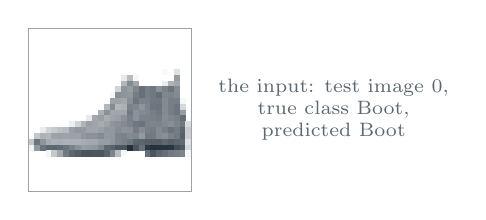
\begin{tikzpicture}[x=0.74mm,y=0.74mm]
  \fill[cInk!3] (23.00,-7.00) rectangle ++(1.04,-1.04);
\fill[cInk!15] (25.00,-7.00) rectangle ++(1.04,-1.04);
\fill[cInk!11] (16.00,-8.00) rectangle ++(1.04,-1.04);
\fill[cInk!33] (17.00,-8.00) rectangle ++(1.04,-1.04);
\fill[cInk!4] (18.00,-8.00) rectangle ++(1.04,-1.04);
\fill[cInk!47] (25.00,-8.00) rectangle ++(1.04,-1.04);
\fill[cInk!35] (16.00,-9.00) rectangle ++(1.04,-1.04);
\fill[cInk!56] (17.00,-9.00) rectangle ++(1.04,-1.04);
\fill[cInk!43] (18.00,-9.00) rectangle ++(1.04,-1.04);
\fill[cInk!9] (23.00,-9.00) rectangle ++(1.04,-1.04);
\fill[cInk!36] (24.00,-9.00) rectangle ++(1.04,-1.04);
\fill[cInk!42] (25.00,-9.00) rectangle ++(1.04,-1.04);
\fill[cInk!21] (15.00,-10.00) rectangle ++(1.04,-1.04);
\fill[cInk!51] (16.00,-10.00) rectangle ++(1.04,-1.04);
\fill[cInk!47] (17.00,-10.00) rectangle ++(1.04,-1.04);
\fill[cInk!58] (18.00,-10.00) rectangle ++(1.04,-1.04);
\fill[cInk!69] (19.00,-10.00) rectangle ++(1.04,-1.04);
\fill[cInk!62] (20.00,-10.00) rectangle ++(1.04,-1.04);
\fill[cInk!65] (21.00,-10.00) rectangle ++(1.04,-1.04);
\fill[cInk!53] (22.00,-10.00) rectangle ++(1.04,-1.04);
\fill[cInk!60] (23.00,-10.00) rectangle ++(1.04,-1.04);
\fill[cInk!66] (24.00,-10.00) rectangle ++(1.04,-1.04);
\fill[cInk!55] (25.00,-10.00) rectangle ++(1.04,-1.04);
\fill[cInk!4] (14.00,-11.00) rectangle ++(1.04,-1.04);
\fill[cInk!54] (15.00,-11.00) rectangle ++(1.04,-1.04);
\fill[cInk!51] (16.00,-11.00) rectangle ++(1.04,-1.04);
\fill[cInk!50] (17.00,-11.00) rectangle ++(1.04,-1.04);
\fill[cInk!63] (18.00,-11.00) rectangle ++(1.04,-1.04);
\fill[cInk!69] (19.00,-11.00) rectangle ++(1.04,-1.04);
\fill[cInk!62] (20.00,-11.00) rectangle ++(1.04,-1.04);
\fill[cInk!65] (21.00,-11.00) rectangle ++(1.04,-1.04);
\fill[cInk!70] (22.00,-11.00) rectangle ++(1.04,-1.04);
\fill[cInk!58] (23.00,-11.00) rectangle ++(1.04,-1.04);
\fill[cInk!59] (24.00,-11.00) rectangle ++(1.04,-1.04);
\fill[cInk!56] (25.00,-11.00) rectangle ++(1.04,-1.04);
\fill[cInk!45] (14.00,-12.00) rectangle ++(2.04,-1.04);
\fill[cInk!42] (16.00,-12.00) rectangle ++(1.04,-1.04);
\fill[cInk!54] (17.00,-12.00) rectangle ++(1.04,-1.04);
\fill[cInk!66] (18.00,-12.00) rectangle ++(1.04,-1.04);
\fill[cInk!60] (19.00,-12.00) rectangle ++(1.04,-1.04);
\fill[cInk!61] (20.00,-12.00) rectangle ++(1.04,-1.04);
\fill[cInk!65] (21.00,-12.00) rectangle ++(2.04,-1.04);
\fill[cInk!56] (23.00,-12.00) rectangle ++(1.04,-1.04);
\fill[cInk!62] (24.00,-12.00) rectangle ++(2.04,-1.04);
\fill[cInk!4] (26.00,-12.00) rectangle ++(1.04,-1.04);
\fill[cInk!35] (13.00,-13.00) rectangle ++(1.04,-1.04);
\fill[cInk!55] (14.00,-13.00) rectangle ++(1.04,-1.04);
\fill[cInk!35] (15.00,-13.00) rectangle ++(1.04,-1.04);
\fill[cInk!37] (16.00,-13.00) rectangle ++(1.04,-1.04);
\fill[cInk!60] (17.00,-13.00) rectangle ++(1.04,-1.04);
\fill[cInk!58] (18.00,-13.00) rectangle ++(1.04,-1.04);
\fill[cInk!51] (19.00,-13.00) rectangle ++(1.04,-1.04);
\fill[cInk!59] (20.00,-13.00) rectangle ++(1.04,-1.04);
\fill[cInk!66] (21.00,-13.00) rectangle ++(1.04,-1.04);
\fill[cInk!67] (22.00,-13.00) rectangle ++(1.04,-1.04);
\fill[cInk!56] (23.00,-13.00) rectangle ++(1.04,-1.04);
\fill[cInk!62] (24.00,-13.00) rectangle ++(1.04,-1.04);
\fill[cInk!66] (25.00,-13.00) rectangle ++(1.04,-1.04);
\fill[cInk!19] (26.00,-13.00) rectangle ++(1.04,-1.04);
\fill[cInk!38] (12.00,-14.00) rectangle ++(1.04,-1.04);
\fill[cInk!53] (13.00,-14.00) rectangle ++(1.04,-1.04);
\fill[cInk!43] (14.00,-14.00) rectangle ++(3.04,-1.04);
\fill[cInk!64] (17.00,-14.00) rectangle ++(1.04,-1.04);
\fill[cInk!53] (18.00,-14.00) rectangle ++(1.04,-1.04);
\fill[cInk!56] (19.00,-14.00) rectangle ++(1.04,-1.04);
\fill[cInk!58] (20.00,-14.00) rectangle ++(1.04,-1.04);
\fill[cInk!62] (21.00,-14.00) rectangle ++(1.04,-1.04);
\fill[cInk!65] (22.00,-14.00) rectangle ++(1.04,-1.04);
\fill[cInk!56] (23.00,-14.00) rectangle ++(1.04,-1.04);
\fill[cInk!62] (24.00,-14.00) rectangle ++(1.04,-1.04);
\fill[cInk!66] (25.00,-14.00) rectangle ++(1.04,-1.04);
\fill[cInk!47] (26.00,-14.00) rectangle ++(1.04,-1.04);
\fill[cInk!10] (10.00,-15.00) rectangle ++(1.04,-1.04);
\fill[cInk!42] (11.00,-15.00) rectangle ++(1.04,-1.04);
\fill[cInk!46] (12.00,-15.00) rectangle ++(1.04,-1.04);
\fill[cInk!39] (13.00,-15.00) rectangle ++(1.04,-1.04);
\fill[cInk!44] (14.00,-15.00) rectangle ++(1.04,-1.04);
\fill[cInk!46] (15.00,-15.00) rectangle ++(1.04,-1.04);
\fill[cInk!53] (16.00,-15.00) rectangle ++(1.04,-1.04);
\fill[cInk!61] (17.00,-15.00) rectangle ++(1.04,-1.04);
\fill[cInk!53] (18.00,-15.00) rectangle ++(1.04,-1.04);
\fill[cInk!60] (19.00,-15.00) rectangle ++(2.04,-1.04);
\fill[cInk!61] (21.00,-15.00) rectangle ++(1.04,-1.04);
\fill[cInk!63] (22.00,-15.00) rectangle ++(1.04,-1.04);
\fill[cInk!55] (23.00,-15.00) rectangle ++(1.04,-1.04);
\fill[cInk!58] (24.00,-15.00) rectangle ++(1.04,-1.04);
\fill[cInk!61] (25.00,-15.00) rectangle ++(1.04,-1.04);
\fill[cInk!70] (26.00,-15.00) rectangle ++(1.04,-1.04);
\fill[cInk!8] (7.00,-16.00) rectangle ++(1.04,-1.04);
\fill[cInk!21] (8.00,-16.00) rectangle ++(1.04,-1.04);
\fill[cInk!36] (9.00,-16.00) rectangle ++(1.04,-1.04);
\fill[cInk!46] (10.00,-16.00) rectangle ++(1.04,-1.04);
\fill[cInk!44] (11.00,-16.00) rectangle ++(1.04,-1.04);
\fill[cInk!40] (12.00,-16.00) rectangle ++(1.04,-1.04);
\fill[cInk!45] (13.00,-16.00) rectangle ++(1.04,-1.04);
\fill[cInk!51] (14.00,-16.00) rectangle ++(1.04,-1.04);
\fill[cInk!53] (15.00,-16.00) rectangle ++(1.04,-1.04);
\fill[cInk!56] (16.00,-16.00) rectangle ++(1.04,-1.04);
\fill[cInk!60] (17.00,-16.00) rectangle ++(1.04,-1.04);
\fill[cInk!65] (18.00,-16.00) rectangle ++(1.04,-1.04);
\fill[cInk!67] (19.00,-16.00) rectangle ++(1.04,-1.04);
\fill[cInk!60] (20.00,-16.00) rectangle ++(1.04,-1.04);
\fill[cInk!59] (21.00,-16.00) rectangle ++(1.04,-1.04);
\fill[cInk!60] (22.00,-16.00) rectangle ++(1.04,-1.04);
\fill[cInk!56] (23.00,-16.00) rectangle ++(1.04,-1.04);
\fill[cInk!54] (24.00,-16.00) rectangle ++(1.04,-1.04);
\fill[cInk!59] (25.00,-16.00) rectangle ++(1.04,-1.04);
\fill[cInk!65] (26.00,-16.00) rectangle ++(1.04,-1.04);
\fill[cInk!17] (27.00,-16.00) rectangle ++(1.04,-1.04);
\fill[cInk!9] (2.00,-17.00) rectangle ++(1.04,-1.04);
\fill[cInk!21] (3.00,-17.00) rectangle ++(1.04,-1.04);
\fill[cInk!25] (4.00,-17.00) rectangle ++(1.04,-1.04);
\fill[cInk!30] (5.00,-17.00) rectangle ++(1.04,-1.04);
\fill[cInk!33] (6.00,-17.00) rectangle ++(1.04,-1.04);
\fill[cInk!46] (7.00,-17.00) rectangle ++(1.04,-1.04);
\fill[cInk!50] (8.00,-17.00) rectangle ++(1.04,-1.04);
\fill[cInk!48] (9.00,-17.00) rectangle ++(1.04,-1.04);
\fill[cInk!44] (10.00,-17.00) rectangle ++(2.04,-1.04);
\fill[cInk!46] (12.00,-17.00) rectangle ++(1.04,-1.04);
\fill[cInk!50] (13.00,-17.00) rectangle ++(1.04,-1.04);
\fill[cInk!49] (14.00,-17.00) rectangle ++(1.04,-1.04);
\fill[cInk!55] (15.00,-17.00) rectangle ++(1.04,-1.04);
\fill[cInk!52] (16.00,-17.00) rectangle ++(1.04,-1.04);
\fill[cInk!53] (17.00,-17.00) rectangle ++(1.04,-1.04);
\fill[cInk!63] (18.00,-17.00) rectangle ++(1.04,-1.04);
\fill[cInk!55] (19.00,-17.00) rectangle ++(1.04,-1.04);
\fill[cInk!61] (20.00,-17.00) rectangle ++(1.04,-1.04);
\fill[cInk!63] (21.00,-17.00) rectangle ++(1.04,-1.04);
\fill[cInk!56] (22.00,-17.00) rectangle ++(1.04,-1.04);
\fill[cInk!61] (23.00,-17.00) rectangle ++(1.04,-1.04);
\fill[cInk!67] (24.00,-17.00) rectangle ++(1.04,-1.04);
\fill[cInk!63] (25.00,-17.00) rectangle ++(1.04,-1.04);
\fill[cInk!74] (26.00,-17.00) rectangle ++(1.04,-1.04);
\fill[cInk!24] (27.00,-17.00) rectangle ++(1.04,-1.04);
\fill[cInk!27] (1.00,-18.00) rectangle ++(1.04,-1.04);
\fill[cInk!37] (2.00,-18.00) rectangle ++(1.04,-1.04);
\fill[cInk!35] (3.00,-18.00) rectangle ++(1.04,-1.04);
\fill[cInk!44] (4.00,-18.00) rectangle ++(1.04,-1.04);
\fill[cInk!45] (5.00,-18.00) rectangle ++(1.04,-1.04);
\fill[cInk!44] (6.00,-18.00) rectangle ++(1.04,-1.04);
\fill[cInk!45] (7.00,-18.00) rectangle ++(2.04,-1.04);
\fill[cInk!50] (9.00,-18.00) rectangle ++(1.04,-1.04);
\fill[cInk!53] (10.00,-18.00) rectangle ++(2.04,-1.04);
\fill[cInk!56] (12.00,-18.00) rectangle ++(1.04,-1.04);
\fill[cInk!49] (13.00,-18.00) rectangle ++(1.04,-1.04);
\fill[cInk!50] (14.00,-18.00) rectangle ++(1.04,-1.04);
\fill[cInk!59] (15.00,-18.00) rectangle ++(1.04,-1.04);
\fill[cInk!60] (16.00,-18.00) rectangle ++(1.04,-1.04);
\fill[cInk!56] (17.00,-18.00) rectangle ++(1.04,-1.04);
\fill[cInk!58] (18.00,-18.00) rectangle ++(1.04,-1.04);
\fill[cInk!49] (19.00,-18.00) rectangle ++(1.04,-1.04);
\fill[cInk!64] (20.00,-18.00) rectangle ++(2.04,-1.04);
\fill[cInk!56] (22.00,-18.00) rectangle ++(1.04,-1.04);
\fill[cInk!54] (23.00,-18.00) rectangle ++(1.04,-1.04);
\fill[cInk!60] (24.00,-18.00) rectangle ++(1.04,-1.04);
\fill[cInk!64] (25.00,-18.00) rectangle ++(1.04,-1.04);
\fill[cInk!77] (26.00,-18.00) rectangle ++(1.04,-1.04);
\fill[cInk!23] (27.00,-18.00) rectangle ++(1.04,-1.04);
\fill[cInk!27] (0.00,-19.00) rectangle ++(1.04,-1.04);
\fill[cInk!66] (1.00,-19.00) rectangle ++(1.04,-1.04);
\fill[cInk!51] (2.00,-19.00) rectangle ++(1.04,-1.04);
\fill[cInk!41] (3.00,-19.00) rectangle ++(1.04,-1.04);
\fill[cInk!38] (4.00,-19.00) rectangle ++(1.04,-1.04);
\fill[cInk!39] (5.00,-19.00) rectangle ++(1.04,-1.04);
\fill[cInk!37] (6.00,-19.00) rectangle ++(1.04,-1.04);
\fill[cInk!38] (7.00,-19.00) rectangle ++(2.04,-1.04);
\fill[cInk!40] (9.00,-19.00) rectangle ++(1.04,-1.04);
\fill[cInk!42] (10.00,-19.00) rectangle ++(2.04,-1.04);
\fill[cInk!47] (12.00,-19.00) rectangle ++(2.04,-1.04);
\fill[cInk!51] (14.00,-19.00) rectangle ++(1.04,-1.04);
\fill[cInk!58] (15.00,-19.00) rectangle ++(1.04,-1.04);
\fill[cInk!61] (16.00,-19.00) rectangle ++(1.04,-1.04);
\fill[cInk!65] (17.00,-19.00) rectangle ++(1.04,-1.04);
\fill[cInk!75] (18.00,-19.00) rectangle ++(2.04,-1.04);
\fill[cInk!77] (20.00,-19.00) rectangle ++(1.04,-1.04);
\fill[cInk!78] (21.00,-19.00) rectangle ++(2.04,-1.04);
\fill[cInk!73] (23.00,-19.00) rectangle ++(1.04,-1.04);
\fill[cInk!77] (24.00,-19.00) rectangle ++(1.04,-1.04);
\fill[cInk!74] (25.00,-19.00) rectangle ++(1.04,-1.04);
\fill[cInk!72] (26.00,-19.00) rectangle ++(1.04,-1.04);
\fill[cInk!14] (27.00,-19.00) rectangle ++(1.04,-1.04);
\fill[cInk!6] (0.00,-20.00) rectangle ++(1.04,-1.04);
\fill[cInk!49] (1.00,-20.00) rectangle ++(1.04,-1.04);
\fill[cInk!67] (2.00,-20.00) rectangle ++(1.04,-1.04);
\fill[cInk!74] (3.00,-20.00) rectangle ++(2.04,-1.04);
\fill[cInk!72] (5.00,-20.00) rectangle ++(1.04,-1.04);
\fill[cInk!67] (6.00,-20.00) rectangle ++(1.04,-1.04);
\fill[cInk!60] (7.00,-20.00) rectangle ++(1.04,-1.04);
\fill[cInk!53] (8.00,-20.00) rectangle ++(1.04,-1.04);
\fill[cInk!47] (9.00,-20.00) rectangle ++(1.04,-1.04);
\fill[cInk!49] (10.00,-20.00) rectangle ++(1.04,-1.04);
\fill[cInk!50] (11.00,-20.00) rectangle ++(1.04,-1.04);
\fill[cInk!57] (12.00,-20.00) rectangle ++(1.04,-1.04);
\fill[cInk!73] (13.00,-20.00) rectangle ++(1.04,-1.04);
\fill[cInk!76] (14.00,-20.00) rectangle ++(1.04,-1.04);
\fill[cInk!82] (15.00,-20.00) rectangle ++(2.04,-1.04);
\fill[cInk!100] (17.00,-20.00) rectangle ++(1.04,-1.04);
\fill[cInk!82] (18.00,-20.00) rectangle ++(1.04,-1.04);
\fill[cInk!69] (19.00,-20.00) rectangle ++(1.04,-1.04);
\fill[cInk!96] (20.00,-20.00) rectangle ++(1.04,-1.04);
\fill[cInk!99] (21.00,-20.00) rectangle ++(1.04,-1.04);
\fill[cInk!98] (22.00,-20.00) rectangle ++(2.04,-1.04);
\fill[cInk!97] (24.00,-20.00) rectangle ++(1.04,-1.04);
\fill[cInk!86] (25.00,-20.00) rectangle ++(1.04,-1.04);
\fill[cInk!81] (26.00,-20.00) rectangle ++(1.04,-1.04);
\fill[cInk!19] (27.00,-20.00) rectangle ++(1.04,-1.04);
\fill[cInk!5] (3.00,-21.00) rectangle ++(1.04,-1.04);
\fill[cInk!26] (4.00,-21.00) rectangle ++(1.04,-1.04);
\fill[cInk!42] (5.00,-21.00) rectangle ++(1.04,-1.04);
\fill[cInk!64] (6.00,-21.00) rectangle ++(1.04,-1.04);
\fill[cInk!73] (7.00,-21.00) rectangle ++(1.04,-1.04);
\fill[cInk!78] (8.00,-21.00) rectangle ++(1.04,-1.04);
\fill[cInk!82] (9.00,-21.00) rectangle ++(1.04,-1.04);
\fill[cInk!83] (10.00,-21.00) rectangle ++(1.04,-1.04);
\fill[cInk!82] (11.00,-21.00) rectangle ++(2.04,-1.04);
\fill[cInk!75] (13.00,-21.00) rectangle ++(1.04,-1.04);
\fill[cInk!59] (14.00,-21.00) rectangle ++(1.04,-1.04);
\fill[cInk!32] (15.00,-21.00) rectangle ++(1.04,-1.04);
\fill[cInk!3] (16.00,-21.00) rectangle ++(1.04,-1.04);
\fill[cInk!70] (20.00,-21.00) rectangle ++(1.04,-1.04);
\fill[cInk!82] (21.00,-21.00) rectangle ++(1.04,-1.04);
\fill[cInk!74] (22.00,-21.00) rectangle ++(1.04,-1.04);
\fill[cInk!69] (23.00,-21.00) rectangle ++(1.04,-1.04);
\fill[cInk!64] (24.00,-21.00) rectangle ++(1.04,-1.04);
\fill[cInk!62] (25.00,-21.00) rectangle ++(1.04,-1.04);
\fill[cInk!59] (26.00,-21.00) rectangle ++(1.04,-1.04);
\fill[cInk!4] (27.00,-21.00) rectangle ++(1.04,-1.04);
\draw[cInk!45,line width=0.3pt] (0.00,0.00) rectangle ++(28,-28);

  \node[note,anchor=west] at (31,-14) {the input: test image 0,\\true class \trueClass,\\predicted \predClass};
\end{tikzpicture}

\vspace{1mm}
\raggedright\footnotesize
\begin{itemize}
  \item Nobody designed these kernels: they began as random numbers and were shaped by gradient descent
        on \nTrain{} labelled images (experiment J; ordered by mean activation on this image).
  \item \mapSparsity\% of the values in the eight maps are exactly zero after ReLU: a map marks
        \emph{where} its pattern occurs and is silent elsewhere.
  \item In this run, maps 1 and 2 fire on the empty background, map 3 on the sole (a horizontal edge),
        maps 4 and 7 on the vertical edge at the back of the shaft.
  \item The kernels are noisier than textbook pictures; the familiar clean oriented-edge filters come
        from much larger networks and datasets \cite{4,12}. Deeper layers combine these maps into
        detectors for larger parts.
\end{itemize}
\end{columns}
\end{frame}

% ====================================================================== 19
\begin{frame}{Four networks that shaped the field}
\centering
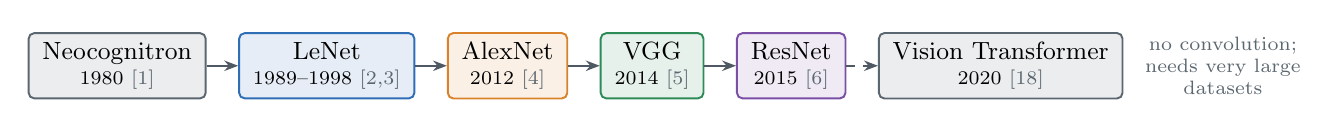
\begin{tikzpicture}[node distance=4mm,font=\footnotesize]
  \node[stage=cTok] (neo) {Neocognitron\\[-2pt]{\scriptsize 1980 \cite{1}}};
  \node[stage=cEmb,right=of neo] (lenet) {LeNet\\[-2pt]{\scriptsize 1989--1998 \cite{2,3}}};
  \node[stage=cAtt,right=of lenet] (alex) {AlexNet\\[-2pt]{\scriptsize 2012 \cite{4}}};
  \node[stage=cFfn,right=of alex] (vgg) {VGG\\[-2pt]{\scriptsize 2014 \cite{5}}};
  \node[stage=cOut,right=of vgg] (res) {ResNet\\[-2pt]{\scriptsize 2015 \cite{6}}};
  \node[stage=cTok,right=of res] (vit) {Vision Transformer\\[-2pt]{\scriptsize 2020 \cite{18}}};
  \draw[flow] (neo)--(lenet); \draw[flow] (lenet)--(alex); \draw[flow] (alex)--(vgg); \draw[flow] (vgg)--(res);
  \draw[flow,dashed] (res)--(vit);
  \node[note,right=1.5mm of vit,anchor=west] {no convolution;\\needs very large\\datasets};
\end{tikzpicture}

\vspace{1.5mm}
\begin{columns}[T,onlytextwidth]
\column{0.60\textwidth}
{\footnotesize
\renewcommand{\arraystretch}{1.15}
\begin{tabular}{@{}llrrl@{}}
\toprule
network & year & weight layers & parameters & ImageNet top-5 error\\
\midrule
LeNet-5 \cite{3} & 1998 & 7 & 60 thousand & n/a (MNIST digits)\\
AlexNet \cite{4} & 2012 & 8 & 60 million & 15.3\%\\
VGG-16 \cite{5} & 2014 & 16 & 138 million & 7.3\%\\
ResNet-152 \cite{6} & 2015 & 152 & 60 million & 3.57\%\\
\bottomrule
\end{tabular}}

\vspace{0.3mm}
{\scriptsize\color{cTok}Layers counted as in each paper. Top-5 test error of the ImageNet competition entries (ensembles). Quoted, not measured here.}

\vspace{0.8mm}
\footnotesize
\begin{itemize}
  \item \key{LeNet}: convolution, subsampling and dense layers trained end to end by backpropagation, to read
        handwritten digits. The template for slide 11.
  \item \key{AlexNet}: the same idea scaled up, with ReLU, dropout, augmentation and GPUs.
        Its 2012 ImageNet win started the deep-learning era in vision.
  \item \key{VGG}: depth matters. Only $3\times3$ convolutions, stacked (slide 6), and $2\times2$ max-pooling.
  \item \key{ResNet}: residual connections make very deep networks trainable; batch norm after every
        convolution; global average pooling as the head.
\end{itemize}
\column{0.37\textwidth}
\centering
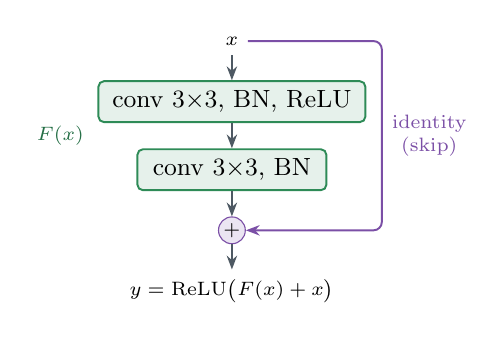
\begin{tikzpicture}[font=\scriptsize,node distance=3.2mm]
  \node (x) {$x$};
  \node[stage=cFfn,below=of x,minimum height=5.2mm,minimum width=24mm] (c1) {conv $3{\times}3$, BN, ReLU};
  \node[stage=cFfn,below=of c1,minimum height=5.2mm,minimum width=24mm] (c2) {conv $3{\times}3$, BN};
  \node[circle,draw=cOut,fill=cOut!15,inner sep=0.6pt,below=of c2] (add) {$+$};
  \node[below=3.2mm of add] (y) {$y=\ReLU\bigl(F(x)+x\bigr)$};
  \draw[flow] (x)--(c1); \draw[flow] (c1)--(c2); \draw[flow] (c2)--(add); \draw[flow] (add)--(y);
  \draw[flow,cOut,rounded corners=3pt] (x.east) -- ++(17mm,0) |- node[pos=0.25,right,note,text=cOut] {identity\\(skip)} (add.east);
  \node[note,left=0.5mm of c1,yshift=-4.3mm,text=cFfn!80!black] {$F(x)$};
\end{tikzpicture}

\vspace{0.5mm}
\begin{block}{Residual connection}
\footnotesize
Very deep plain networks had \emph{higher training error} than shallower ones \cite{6}:
an optimisation failure, not overfitting. A residual block learns only the change $F(x)$ to its input.
Doing nothing ($F=0$) is easy, and gradients reach early layers directly through the skip path.
\end{block}
\end{columns}
\end{frame}

% ====================================================================== 20
\begin{frame}{References and how to run the code}
\fontsize{6.4}{7.9}\selectfont
\begin{columns}[T,onlytextwidth]
\column{0.49\textwidth}
\begin{enumerate}[{[1]}]\setlength{\itemsep}{0.6pt}
\item Fukushima. \emph{Neocognitron: A Self-organizing Neural Network Model for a Mechanism of Pattern Recognition Unaffected by Shift in Position.} Biological Cybernetics 36, 1980.
\item LeCun, Boser, Denker, Henderson, Howard, Hubbard, Jackel. \emph{Backpropagation Applied to Handwritten Zip Code Recognition.} Neural Computation 1(4), 1989.
\item LeCun, Bottou, Bengio, Haffner. \emph{Gradient-Based Learning Applied to Document Recognition.} Proceedings of the IEEE 86(11), 1998.
\item Krizhevsky, Sutskever, Hinton. \emph{ImageNet Classification with Deep Convolutional Neural Networks.} NeurIPS 2012.
\item Simonyan, Zisserman. \emph{Very Deep Convolutional Networks for Large-Scale Image Recognition.} ICLR 2015. arXiv:1409.1556
\item He, Zhang, Ren, Sun. \emph{Deep Residual Learning for Image Recognition.} CVPR 2016. arXiv:1512.03385
\item Ioffe, Szegedy. \emph{Batch Normalization: Accelerating Deep Network Training by Reducing Internal Covariate Shift.} ICML 2015. arXiv:1502.03167
\item Srivastava, Hinton, Krizhevsky, Sutskever, Salakhutdinov. \emph{Dropout: A Simple Way to Prevent Neural Networks from Overfitting.} JMLR 15, 2014.
\item Kingma, Ba. \emph{Adam: A Method for Stochastic Optimization.} ICLR 2015. arXiv:1412.6980
\item Lin, Chen, Yan. \emph{Network In Network.} ICLR 2014. arXiv:1312.4400
\item Dumoulin, Visin. \emph{A Guide to Convolution Arithmetic for Deep Learning.} 2016. arXiv:1603.07285
\item Zeiler, Fergus. \emph{Visualizing and Understanding Convolutional Networks.} ECCV 2014. arXiv:1311.2901
\end{enumerate}
\column{0.49\textwidth}
\begin{enumerate}[{[1]}]\setlength{\itemsep}{0.6pt}
\setcounter{enumi}{12}
\item Xiao, Rasul, Vollgraf. \emph{Fashion-MNIST: a Novel Image Dataset for Benchmarking Machine Learning Algorithms.} 2017. arXiv:1708.07747. Data: github.com/zalandoresearch/fashion-mnist
\item Goodfellow, Bengio, Courville. \emph{Deep Learning}, chapter 9. MIT Press, 2016. deeplearningbook.org
\item Azulay, Weiss. \emph{Why Do Deep Convolutional Networks Generalize so Poorly to Small Image Transformations?} JMLR 20, 2019. arXiv:1805.12177
\item Luo, Li, Urtasun, Zemel. \emph{Understanding the Effective Receptive Field in Deep Convolutional Neural Networks.} NeurIPS 2016. arXiv:1701.04128
\item Sobel, Feldman. \emph{A 3x3 Isotropic Gradient Operator for Image Processing.} Talk, Stanford Artificial Intelligence Project, 1968.
\item Dosovitskiy et al. \emph{An Image is Worth 16x16 Words: Transformers for Image Recognition at Scale.} ICLR 2021. arXiv:2010.11929
\item Paszke et al. \emph{PyTorch: An Imperative Style, High-Performance Deep Learning Library.} NeurIPS 2019. arXiv:1912.01703
\end{enumerate}

\vspace{0.5mm}
{\fontsize{6.5}{7.9}\selectfont\color{cInk}
\textbf{Run it} (Python, NumPy, PyTorch; CPU only)

\vspace{0.5mm}
\begin{tabular}{@{}l>{\raggedright\arraybackslash}p{52mm}@{}}
\texttt{python test\_cnn.py} & seven checks, incl.\ backward pass vs.\ finite differences\\
\texttt{python walkthrough.py} & the hand calculations (slides 2--10, 12, 14)\\
\texttt{python conv\_numpy.py} & from-scratch convolution vs.\ PyTorch\\
\texttt{python train.py} & the harness, about a minute; \texttt{-{}-help} lists every knob\\
\texttt{python experiments.py} & all figures and numbers, about \totalMinutes{} minutes\\
\end{tabular}

\vspace{0.6mm}
\textbf{Exercises.} Train \texttt{-{}-model cnn\_gap} and compare parameters and accuracy.
Replace max- by average-pooling. Test the augmented CNN at a 6-pixel shift.}
\end{columns}
\end{frame}

\end{document}
